%------------------------------------------------------------------------
%                           DISCUS Users guide
%------------------------------------------------------------------------

\documentclass[11pt]{report}

\usepackage[letterpaper]{geometry}
\geometry{height=8.5in}
\geometry{bottom=1.1in}
\geometry{left=1.1in}
\geometry{right=1.1in}

\usepackage[dvips]{graphicx}
\usepackage{fancyhdr}
\usepackage{floatflt}
\usepackage{tabularx}
\usepackage[round]{natbib}
\usepackage[hang,small,bf]{caption}
\usepackage{fancyvrb}
\usepackage{scalefnt}
\usepackage{color}
\usepackage{url}
\usepackage{hyperref}

\usepackage[T1]{fontenc}
\usepackage{palatino}

\newcommand{\version}{5.27}

\newcommand{\discus}{\textsc{Discus}}
\newcommand{\Discus}{\textsc{Discus\ }}
\newcommand{\kuplot}{\textsc{Kuplot}}
\newcommand{\Kuplot}{\textsc{Kuplot\ }}
\newcommand{\diffev}{\textsc{Diffev}}
\newcommand{\Diffev}{\textsc{Diffev\ }}
\newcommand{\Suite}{\textsc{Discus Suite\ }}
\newcommand{\suite}{\textsc{Discus Suite}}

% General page style

\pagestyle{fancy}
\fancyhf{}
\fancyhead[L]{\bfseries \slshape\leftmark}
\fancyhead[R]{\bfseries Users Guide}
\fancyfoot[R]{\bfseries Page \thepage}
\fancyfoot[L]{\bfseries \Discus \version}
\renewcommand{\footrulewidth}{0.4pt}
\renewcommand{\headrulewidth}{0.4pt}

% Style for chapter start pages ..

\fancypagestyle{plain} {
  \fancyhf{}
  \fancyhead[R]{\bfseries Users Guide}
  \fancyfoot[L]{\bfseries \Discus \version}
  \fancyfoot[R]{\bfseries Page \thepage}
  \renewcommand{\headrulewidth}{0.4pt}
}

% MacVerbatim style for macros

\definecolor{DarkBlue}{rgb}{0.1,0.0,0.5}

\DefineVerbatimEnvironment%
{MacVerbatim}{Verbatim}
{fontfamily=courier,
 fontsize=\scriptsize,
 fontseries=b,
 formatcom=\color{DarkBlue}}

\graphicspath{{pic/}}

\setlength\parindent{0pt}

%------------------------------------------------------------------------

\begin{document}

%------------------------------------------------------------------------
% Title
%------------------------------------------------------------------------

\begin{titlepage}
\begin{flushright}

  \hrule
  \vspace{15mm}
  \textbf{{\scalefont{8} \discus}} \\
  \vspace{15mm}
  \textbf{{\scalefont{4} Users Guide}} \\
  \vspace{10mm}
  \textbf{{\Huge Version  \version}} \\
  \vspace{10mm}

  \hrule
  \vspace{40mm}
  \textbf{written by} \\

  \vspace{5mm}
  \textbf{\Large Reinhard Neder} \\
  Email: reinhard.neder@fau.de \\

  \vspace{ 2mm}
  \textbf{\Large Thomas Proffen} \\
  Email: tproffen@ornl.gov \\

  \vspace{12mm}
  \textbf{\Large \url{http://tproffen.github.io/DiffuseCode}} \\

  \vspace{3mm}
  \hrule

\end{flushright}
\begin{flushright}
  \textit{Document created: \today}
\end{flushright}

\end{titlepage}

%------------------------------------------------------------------------
% Preface
%------------------------------------------------------------------------

\chapter*{Preface}
\subsection*{Disclaimer}

The \Discus software described in this guide is
provided without warranty of any kind.  No liability is taken for any loss
or damages, direct or indirect, that may result through the use of \discus.
No warranty is made with respect to this manual, or the program
and functions therein.  There are no warranties that the programs are free
of error, or that they are consistent with any standard, or that they will
meet the requirement for a particular application.  The programs and the
manual have been thoroughly checked.  Nevertheless, it can not be
guaranteed that the manual is correct and up-to-date in every detail. This
manual and the \Discus program may be changed without notice.\par

\Discus is intended as a public domain program.  It may be used free
of charge.  Any commercial use is, however, not allowed without the
explicit written permission of the authors.

%------------------------------------------------------------------------

\subsection*{Acknowledgments}

The parameters for the calculation of bond valence sums were compiled by I.D.
Brown, McMaster University, Hamilton, ON, Canada.

%------------------------------------------------------------------------

\subsection*{Using DISCUS}

Publication of results totally or partially obtained using the program 
\Discus should state that \Discus was used and contain the following
reference:

\begin{quote}
  {\sc Proffen, Th. \& Neder, R.B.} (1997) "DISCUS, a Program
  for Diffuse Scattering and Defect Structure Simulations"
  {\it J. Appl. Cryst.}, {\bf 30}, 171-175
\end{quote}

%------------------------------------------------------------------------

\newpage
\subsection*{More information}

This users guide can only provide program specific details. A
broader discussion of simulation techniques and many \Discus
examples and macro files can be found in our book

\begin{quote}
  {\sc Neder, R.B. \& Proffen, Th.} "Diffuse Scattering and Defect Structure
  Simulations - A cook book using the programs DISCUS", {\it IUCr Texts on
  Crystallography}, Oxford University Press, 2008.
\end{quote}

%\begin{figure}[!t]
%   \centering
%   \includegraphics[width=0.5\linewidth]{cookbook.eps}
%   \vspace{10mm}
%\end{figure}

The macro files used in the cookbook can also be downloaded to the 
\Discus homepage at \url{https://github.com/tproffen/DiscusCookBookExamples}.

%------------------------------------------------------------------------
% Table of contents, List of Tables etc..
%------------------------------------------------------------------------

\tableofcontents
%\listoffigures
%\listoftables

%------------------------------------------------------------------------
% Here all the chapter are included ...
%
% Alter or comment the \includeonly command above to work with the
% complete manual or only certain parts.
%
%------------------------------------------------------------------------

%------------------------------------------------------------------------
% Chapter:  Introduction
%------------------------------------------------------------------------

\chapter{Introduction}
\section{What is DISCUS ?}

\Discus \citep{prne97} is intended as a versatile tool to
simulate crystal structures and the corresponding intensity
distribution in reciprocal space.  The program offers several
features that enable the user to easily generate a structure and
to introduce various defects.  The main intend is to simulate
defect structures, the program, however, is not limited in that
respect.  Ideal structures can be simulated as well and usually
will form the basis from which the defect structure is developed.
\par

The program can read a whole crystal or the asymmetric unit of a
unit cell. The latter is expanded to the whole unit cell by use of
the space group symbol. The definition of rigid molecules is
supported by \discus. The structure can be stored as structure
file or certain layers or projections of the crystal can be saved
for graphical display. The program \Discus is part of the
diffuse program package. Several tools are available to
modify single atoms or molecules within the structure or to alter
the complete crystal. These tools include thermal displacements,
waves, domains, stacking faults and generalized symmetry
operations. One feature of \Discus is the possibility to
introduce correlated defects and distortions using Monte Carlo (MC)
simulations. Various tools allow the analysis of a given defect
structure including the calculation of the PDF of a given structure.
\par

The Fourier transform segment of the program allows the user to
calculate  the intensity distribution along a line, arbitrarily 
oriented plane or a three dimensional volume
through reciprocal space. The resolution in reciprocal space can be
chosen by the user. The resulting intensity maps can be written in
several output formats, to be displayed by standard visualization
programs, the program {\it KUPLOT} or be printed directly.
The list of output formats includes the NeXus format.  Neutron-
as well as X-ray and electron scattering can be calculated. 
\Discus supports
the subtraction of the average structure factor and the calculation
of the diffuse intensities as average over many small crystal
volumes to create smooth noise free diffraction pattern. A detailed
discussion is given in chapter \ref{four}. The direct analysis of
measured diffuse scattering is possible using the Reverse Monte
Carlo segment of the program. The program allows the refinement of
the scattering intensity directly as well as the refinement of the
PDF. \par

The program uses a command language to interact with the user. No
predefined requirement exists for a given sequence of commands. The
commands can be typed at the \Discus prompt, or read from a
macro file. The command language includes a FORTRAN style
interpreter that allows the user to program loops and logical
structures. Several real and integer variables as well as structural
variables can be used to design the intended defect structure. On
line help is provided which gives the user information on any of the
\Discus commands as well as examples for typical \Discus
sessions. More detailed information how to get further help is given
in section \ref{get}.

%------------------------------------------------------------------------

\section{Getting started \label{get}}

After the program \Discus is installed properly and the environment
variables are set, the program can be started by typing 'discus' at the
operating systems prompt. Information about the installation of \Discus
is given in the \Discus package manual.

The program uses a command language to interact with the user.  The
command {\tt exit} terminates the program and returns control to the
shell.  All commands of \Discus consist of a command verb,
optionally followed by one or more parameters.  All parameters must
be separated from one another by a comma ",".  There is no
predefined need for any specific sequence of commands.  \Discus
is case sensitive, all commands and alphabetic parameters MUST be
typed in lower case letters.  If \Discus has been compiled
using the {\tt -DREADLINE} option (see installation files) basic
line editing and recall of commands is possible.  For more
information refer to the reference manual or check the online help
using ('help command input').  Names of input or output files are to
be typed as they will be expected by the shell.  If necessary
include a path to the file.  All commands may be abbreviated to the
shortest unique possibility. At least a single space is needed
between the command verb and the first parameter.  No comma is to
precede the first parameter. A line can be marked as comment by
inserting a "{\tt \#}" as first character in the line.\par

The symbols used throughout this manual to describe commands,
command parameters, or explicit text used by the program \Discus 
are listed in Table \ref{sym-tab}. There are several sources
of information, first \Discus has a build in online help, which
can be accessed by entering the command {\tt help} or if help for a
particular command $<$cmd$>$ is wanted by {\tt help $<$cmd$>$}. This
manual describes background and principle functions of \Discus
and should give some insight in the ways to use this program. \par

\begin{table}[!tbh]
\centering
\begin{tabularx}{\textwidth}{|p{30mm}|X|}
  \hline
  {\bf Symbol} & {\bf Description} \\
  \hline\hline
  "text"     &  Text given in double quotes is to be understood as typed. \\
  \hline
  $<$text$>$ &  Text given in angled brackets is to be replaced by an
                appropriate value, if the corresponding line is used
                in \Discus. It could, for example be the actual name
                of a file, or a numerical value. \\
  \hline
  {\tt text} &  Text in single quotes exclusively refers to \Discus
                commands. \\
  \hline
  $[$text$]$ &  Text in square brackets describes an optional parameter or
                command. If omitted, a default value is used, else
                the complete text given in the square brackets is to
                be typed. \\
  \hline
  \{text $|$ text\} &  Text given in curly brackets is a list of alternative
                parameters. A vertical line separates two alternative,
                mutually exclusive parameters. \\
  \hline
\end{tabularx}
\caption{\label{sym-tab}Used symbols}
\end{table}

As we have mentioned before, \Discus is controlled by a powerful command
language which is common to all programs in the \Discus package. 
A detailed description of the command language can be found in the 
\Discus Reference Guide which is included in the distribution.
Variables specific to the program \Discus are shown in Tables 
\ref{v1-tab} and \ref{v2-tab}. \Discus also provides a number of structure
related functions which are listed in Tab. \ref{func-cryst} and
\ref{func-cryst2}.

\begin{table}[!tbh]
\centering
\begin{tabularx}{\textwidth}{|p{30mm}|X|}
  \hline
  {\bf Variable} & {\bf Description} \\
  \hline\hline
  n[1]      & Number of atoms within the crystal \\
  n[2]      & Number of different scattering types, i.e. atoms \\
  n[3]      & Number of atoms within the unit cell \\
  n[4]      & Number of molecules within the crystal \\
  n[5]      & Number of different molecule types \\
  n[6]      & Number of molecules within the unit cell \\
  n[7]      & Number of none-void atoms in the crystal \\
  \hline
  cdim[i,1] & Lowest coordinate of any atom (i=1,2,3 for x,y,z) \\
  cdim[i,2] & Highest coordinate of any atom (i=1,2,3 for x,y,z) \\
  \hline\hline
  env[i]    & Index of neighboring atoms after 'find' command \\
  menv[i]   & Index of neighboring molecules after 'find' command \\
  \hline\hline
  lat[i]    & Lattice parameters \
              (i=1..6 for $a,b,c,\alpha,\beta,\gamma$\\
  vol[1]    & Unit cell volume \\
  rvol[1]   & Reciprocal unit cell volume \\
  \hline
\end{tabularx}
\caption{\label{v1-tab}Crystal related variables}
\end{table}

\begin{table}[!tbh]
\centering
\begin{tabularx}{\textwidth}{|p{30mm}|X|}
  \hline
  {\bf Variable} & {\bf Description} \\
  \hline\hline
  m[i]   & Number of scattering type (i.e. atom type) for atom i \\
  b[i]   & isotropic thermal factor B for atom {\bf type} i \\
  occ[i]   & occupancy parameter for atom {\bf type} i \\
  at\_name[i] & Atom name for atom i\\
  in\_mole[i] & Molecule in which atom i is \\
  prop    [i] & Property of atom i \\
  \hline
  at\_type[i] & Atom name for atom type i\\
  \hline
  x[i]   & fractional x position of atom i \\
  y[i]   & fractional y position of atom i \\ 
  z[i]   & fractional z position of atom i \\
  \hline\hline
  mol\_cont[i,j] & Index of atom j in molecule i \\
  mol\_len[i]    & Number of atoms in molecule i \\
  mol\_biso[i]   & Isotropic B-value for molecule i\\
  mol\_dens[i]   & Density of object i \\
  mol\_type[i]   & Type of object / molecule / domain i \\ 
  \hline\hline
  pdf\_dens[i]   & Number density for pdf calculations \\
  pdf\_scal[i]   & Scale factor   for pdf calculations \\
  \hline
\end{tabularx}
\caption{\label{v2-tab}Variables related to individual atoms and
         molecules}
\end{table}

\begin{table}[!tbh]
\centering
\begin{tabularx}{\textwidth}{|p{10mm}|p{47mm}|X|}
  \hline
  {\bf Type} & {\bf Name} & {\bf Description} \\
  \hline\hline
  real & \raggedright bang(u1,u2,u3, v1,v2,v3 [,w1,w2,w3]) &
       Returns the bond angle in degrees between {\bf u} and {\bf v}
       at site {\bf w}. If {\bf w} is omitted, the angle between
       direct space vectors {\bf u} and {\bf v} is returned. \\
  real & \raggedright blen(u1,u2,u3 [,v1,v2,v3]) &
       Returns the length of the real space vector {\bf v}-{\bf u}.
       The vector {\bf v} defaults to zero. \\
  real & \raggedright dstar(h1,h2,h3 [,k1,k2,k3]) &
       Returns the length of reciprocal vector {\bf k} - {\bf h} in
       \AA$^{-1}$. Vector {\bf k} defaults to zero. \\
  real & \raggedright rang(h1,h2,h3, k1,k2,k3 [,l1,l2,l3]) &
       Returns the angle between reciprocal vectors {\bf k} - {\bf h} and
       {\bf k} - {\bf l} at site {\bf k}.  If {\bf l} is omitted, the angle
       between reciprocal vectors {\bf h} and {\bf k} is returned. \\
  real & \raggedright scalpro(u1,u2,u3,v1,v2,v3 [,{"dd"|"rr"|"dr"|"rd"}]) &
       Returns the scalar product between the two vectors {\bf u} 
       and {\bf v}.  Both vectors may be given in direct
       or real space coordinates, flagged in parameter no 7. "d" 
       means real space, "r" reciprocal space. \\
  real & \raggedright vprod <u1>,<v1>,<w1>, <u2>,<v2>,<w2> [ ,<flag> ] &
       This is not a function but rather a command that calculates the 
       vector product {\bf 1} X {\bf 2}. The <flag> is a string of three
       characters that indicates whether the input vectors or the output
       vector are given in direct or reciprocal space coordinates. The
       three characters correspond to:

       first input vector,
       second input vector
       resulting vector

       "drd" means: vector one is given in direct space coordinates, vector 2
                is in reciprocal space coordinates (hkl) and the
                resulting vector product is to be given in direct space
                coordinates

       Any combination of "d" and "r" is allowed. \\
  \hline
\end{tabularx}
\caption{\label{func-cryst}Crystallographic functions}
\end{table}


\begin{table}[!tbh]
\begin{tabularx}{\textwidth}{|p{10mm}|p{47mm}|X|}
  \hline
  {\bf Type} & {\bf Name} & {\bf Description} \\
  \hline\hline
   logical & \raggedright isprop(atom [,[and:]property] [,or:property]) &
       Tests if an atom has the property / properties specified by
       property. The test can check a single property, if the 
       property is given by its name as in :

       'normal', 'molecule', 'domain', 'outside', 'external', 'internal',
       'ligand'. 

       Alternatively several properties can be checked 
       simultaneously if the property is a list of capital and/or 
       small letters as in 'NMDOEIL', 'nmdoeil'. A capital letter 
       signifies that the property must be present, a small letter 
       that the property must be absent. 

       The properties in the "and:" parameter must ALL be present, 
       i.e. they are tested with a logical "and". The properties in
       the "or:" parameter are tested with a logical "or", i.e. the
       function is true if any of the listed properties fulfills
       the condition (capital letter==present, small letter==absent).
       At least one of the two parameters must be present. If only 
       one parameter is given and the "and:" is omitted, the default
       is to test with the "and:" condition. \\
  \hline
\end{tabularx}
\caption{\label{func-cryst2}Crystallographic functions continued}
\end{table}

\section{Technical notes \label{tec}}

Most of the time you don not have to worry about the interior 
technical design of \discus. Most of the time the program will 
allocate its required memory and will not need user intervention.
As the command language is designe for utmost flexibility, the 
program will not know if you still need a piece of the allocated
memory or not. Again, most of the time this is not an issue, as 
few section of the program may require huge amount of memory. 
These sections are the Fourier menus (fourier and powder) and
particularly the pdf menu. THe latter can be very memory hungry 
if you deal with meny different atom types and many different 
molecule types. It has been design to 
release temporary memory requirements. As such it should not really
need help with the memory issues. 

The Fourier menus might take up quite a bit of memory, if large
(3-dimensional) sections of reciprocal space are calculated. 
\Discus cannot know if you are done with the final Fourier 
map, After all, you might want to save it in the output menu 
in different formats. This prevents \Discus from a fully 
automatic release of the allocated memory. 

To free all memory, you can use the {\tt reset} command within
any menu or at the \Discus top level. This command will 
free all allocated arrays and furthermore set all menu 
settign back to the default values at program start. 

%------------------------------------------------------------------------

%------------------------------------------------------------------------
% Chapter:  Creating structure
%------------------------------------------------------------------------

\chapter{Creating structures \label{struc}}

The first steps towards any simulation are to create the desired
structure and possibly to modify it.  \Discus offers two
different ways to perform this task, the structure can either be
generated from the contents of a asymmetric unit of a unit cell or
be completely read from a file.  For each atom the program stores
its type, its fractional coordinates (x,y,z) an isotropic
thermal coefficient (B) and a set of property flags. 
 If the crystal is generated from an
asymmetric unit, the program uses the space group symbol read from
the data file to generate the unit cell from the asymmetric unit.
Prior to this generation, the space group symbol is checked for
consistency with the lattice constants.  An error message flags any
inconsistencies.  The unit cell is copied to generate a crystal of
desired (rectangular) dimensions.
\par

The following sections describe the structure file formats and how
to group atoms to (rigid) molecules.  Once a crystal (which could be
as small as one atom) is generated, several tools are provided to
modify the crystal.  These tools can be grouped into those that
affect individual atoms and those that affect the whole crystal.
The first group includes the following modifications of an
individual atom: moving, replacing, removing and inserting new
atoms.  These are discussed in chapter \ref{mod-simple}.  The second
group includes at present the following modifications of the crystal
at large, for more details see chapter \ref{mod}: thermal
displacement, waves, stacking faults and domains, generalized 
symmetry operations ( chapter \ref{cryst}), Monte-Carlo modelling
( chapter \ref{mc}), and Reverse-Monte-Carlo modelling ( chapter 
\ref{rmc}).

%------------------------------------------------------------------------

\section{Reading structure files \label{struc-read}}

\Discus uses its own file format for crystal structures. In part this 
is a legacy feature since the {\it CIF} file format was not around at the time 
\Discus was started. A second aspect concerns the fact that a {\it CIF} file 
is restricted to the content of a single unit cell. As \Discus 
often builds large blocks of unit cells with reduced periodicity, 
the \Discus file format still bears many merits.

For the use of initial input a {\it CIF} file is fine and can be 
read directly 
within the {\tt read} menu. Alternatively the {\it CIF} file can
be imported into the \Discus file format. Further file formats can 
be imported into the \Discus format.

As the standard choice the \Discus 
specific format is described in this section.

A unit cell (actually the asymmetric unit within the unit cell )
or a whole structure is read from file by the command
{\tt read}. The format of these two file types is identical.  If a
unit cell is read, the contents of the file is regarded as the
asymmetric unit of the unit cell.  The space group information is
used to generate the whole unit cell. If, on the other hand, a
structure is read, the contents of the file is taken as it is.  \par

A keyword controlled structure file format is used allowing more
flexibility, e.g. the use of molecules. However, \Discus is
capable to read both the very old and the new structure files
automatically recognizing the correct format. Furthermore the
command {\tt format nokey} in the {\tt save} segment allows the user
to save a structure using the old format (see section
\ref{struc-save}). As the non keyword file format lacks many of
the storage features its use is highly discouraged.


\subsection{Structure file format \label{struc-new}}

The standard \Discus structure file is a simple text file starting
with a section with keywords setting parameters like lattice
constants or space group followed by a section with the actual
atoms. The sequence of keywords is arbitrary with two exceptions,
the first line {\bf must} contain the keyword {\tt title} setting a
title and the last keyword {\bf must} be i{\tt atoms} followed by a list of
atoms and/or molecule definitions (see section \ref{mol}). Each atom
within the asymmetric unit or complete structure is defined 
at least by its
name (e.g. ZR), the fractional coordinates $(x,y,z)$ and an
isotropic temperature factor $B$. The property flag is optional
and defines if the atom is a normal atom, inside a molecule, inside
or outside the crystal, within a domain. 
Starting with version 5.18.0 one can in addition specify the 
molecule number to which the atom belongs and an occupancy for the atom.

A list of valid keywords within a
structure file is given in Table \ref{struc-new-tab1}.

\begin{table}[!tbh]
\centering
\begin{tabularx}{\textwidth}{|p{25mm}|X|}
  \hline
  {\bf Keyword} & {\bf Description} \\
  \hline\hline
  \#          & Allows comments in the keyword section of the structure
                file.. \\
  \hline
  adp         & A list of isotropic B values for all atom types. If 
                present, these values will override the parameter 
                specified for an atom upon reading a structure.\\
  \hline
  atoms       & Marks the start of the atom list and must be the {\bf
                last} keyword except for 'molecule'.\\
              & Parameters are the names of the columns that are 
                present for each atom. Valid columns are:\\
              & x, y, z, Biso:  These four columns must always be present.\\
              & Property:  The property flag\\
              & MoleNo, MoleAt: Molecule number and entry number for the 
                atom. These two columns are written by \Discus during
                a save. To build a structure with molecules it is 
                easier for you to use the {\tt molecule} keyword.\\
              & Occ: Occupancy for this atom type\\
              & The sequence of the columns is arbitrary, yet the recommended
                sequence is:\\
              & x,y,z, Biso, Property, MoleNo, MoleAt, Occ\\
  \hline
  cell        & Parameters $a,b,c,\alpha,\beta,\gamma$ define the
                lattice constants of the crystal. Note that {\bf all} six
                parameters must always be given.\\
  \hline
  generator   & Allows to define generators additional to the ones
                defined by the space group. The 12 parameters define the
                symmetry operation. \\
  \hline
  molecule    & Defines rigid molecules. The keyword must stand in
                the atoms section of the structure file (see section
                \ref{mol}).\\
  \hline
  ncells      & Parameters $nx,ny,nz$ and $nc$ define the size of the
                crystal in unit cells and the number of atoms within a
                unit cell.  This information is needed if a complete
                structure is read in order to allow \Discus to
                determine the crystals size.\\
  \hline
  occ         & A list of atom occupancy values\\
  \hline
  scat        & A list of atom types. This will ensure that the atom
                types have a fixed sequence.\\
  \hline
  spcgr       & Sets the space group for the crystal.\\
  \hline
  symmetry    & Defines an additional symmetry operation defined by
                the 12 parameters given.\\
  \hline
  title       & Sets a title for the structure file. This {\bf must}
                be the first keyword in the file.\\
  \hline
\end{tabularx}
\caption{\label{struc-new-tab1} List of keywords for structure files}
\end{table}

Keywords are processed the same way as normal commands and
parameters have to be separated by commas. An example input file for
cubic zirconia ($ZrO_{2}$) is shown below.

\begin{MacVerbatim}
    title Structure of cubic ZrO2
    spcgr Fm-3m
    cell  5.14, 5.14, 5.14, 90., 90., 90.
    atoms
    ZR    0.00000, 0.00000, 0.00000,  0.5
    O     0.25000, 0.25000, 1./4.  ,  1.0
\end{MacVerbatim}

A full information input file as of version 5.18.0 has the form:

\begin{MacVerbatim}
    title Structure of cubic ZrO2
    spcgr Fm-3m
    cell  5.14, 5.14, 5.14, 90., 90., 90.
    atoms x,    y,    z,     Biso, Property, MoleNo, MoleAt, Occ
    ZR    0.00, 0.00, 0.00,  0.5,  1,        0,      0,      1.0
    O     0.25, 0.25, 1./4., 1.0,  1,        0,      0,      1.0
\end{MacVerbatim}


The first line is the required {\tt title} line describing the
structure. The next line specifies the space group
$Fm\overline{3}m$.  The symbols used should be the Hermann-Mauguin
symbols used in International Tables for Crystallography Vol.  A
\cite{tables}.  A center of inversion as in this example should be
given as {\tt -} sign immediately preceding the axis. Lattice types need
to be given as capital characters, mirror planes as small
characters.  Monoclinic cell choices 2,3 or unique c-axis will be
assumed if the corresponding non standard Hermann-Mauguin symbol is
used. \Discus checks the given space group symbol for
contradictions with the lattice constants and in case of an error
the unit cell is not read.  A complete list of valid space group
symbols is part of the online help and can be accessed via 'help
space' from the \Discus command line.  The next line in the
example above gives the lattice constants of $a=b=c=5.14$\AA \ and
$\alpha=\beta=\gamma=90$ degrees.  Note that \Discus requires
all six values to be given.  The keyword 'atoms' in the example file
which must be the last keyword starts the section with the list of
atoms.  Here zirconium occupies site 4(a) on (0,0,0) and oxygen is
on 8(f) at ($\frac{1}{4}, \frac{1}{4}, \frac{1}{4}$).  The isotropic
temperature factors for Zr and O are set to 0.5 \AA$^{2}$ and 1.0
\AA$^{2}$ respectively. \par

If the lattice parameters or the atom coordinates are separated
by comma, you can use simple expressions like 1./2. or even 
variables instead of explicit numerical values. \par

Additional generators can be defined through the optional {\tt
generator} keyword.  These generators act identical to the
generators defined through the space group symbol.  All previously
generated copies of the atoms in the asymmetric unit are copied by
this generator, and will in turn be copied by any generators
following later.  Since these additional generators are applied
after the space group generators, you can use these generators to
create non-standard groups or to create a set of symmetries that
does not from a group. The syntax of the 'generator' keyword is as
follows:

\begin{MacVerbatim}
    generator g11,g12,g13,g14, g21,g22,g23,g24, g31,g32,g33,g34
\end{MacVerbatim}

Copies of an atom at (x,y,z) will be calculated using the following
equation:

\begin{equation}
        \left ( \begin{array}{c} x'\\ y'\\ z'\end{array} \right ) =
        \left (
        \begin{array}{ccc}
                g_{11} & g_{12} & g_{13}  \\
                g_{21} & g_{22} & g_{23}  \\
                g_{31} & g_{32} & g_{33}
        \end{array}
        \right ) \cdot
        \left ( \begin{array}{c} x\\ y\\ z\end{array} \right ) +
        \left ( \begin{array}{c} g_{14}\\ g_{24}\\ g_{34}\end{array} \right )
        \label{struc-new-eq1}
\end{equation}

Additional symmetry operations can be defined through the optional
{\tt symmetry} keyword.  These symmetry operations act different
than the generators described above which are defined through the
space group symbol or listed as additional generators.  The symmetry
operations copy only those atoms created by the generators.  In
contrast to generators they do not act on copies of the atoms
created by previous symmetry operations. Both keywords {\tt
generator} and {\tt symmetry} define the symmetry operation in a
similar way using 12 parameters as shown in equation
\ref{struc-new-eq1}
\par

The following example shall illustrate the difference between
generators and additional symmetry operations.  The following two
generators

\begin{MacVerbatim}
    generator 1,0,0,0.5, 0,1,0,0.5, 0,0,1,0.0
    generator 1,0,0,0.5, 0,1,0,0.0, 0,0,1,0.5
\end{MacVerbatim}

would create the following copies of an atom at (0,0,0):
$(\frac{1}{2}, \frac{1}{2}, 0), (\frac{1}{2}, 0, \frac{1}{2})$ and
$(0, \frac{1}{2}, \frac{1}{2})$.  In contrast similar symmetry
operations

\begin{MacVerbatim}
    symmetry 1,0,0,0.5, 0,1,0,0.5, 0,0,1,0.0
    symmetry 1,0,0,0.5, 0,1,0,0.0, 0,0,1,0.5
\end{MacVerbatim}

will only generate the following two copies of an atom at (0,0,0):
$(\frac{1}{2}, \frac{1}{2}, 0)$ and $(\frac{1}{2}, 0, \frac{1}{2})$
since the symmetry operations will not act on previously generated
copies of the atom at (0,0,0). The second symmetry operation copies
only the atom at (0,0,0), not the atom at $(\frac{1}{2}, 0,
\frac{1}{2})$, since this atom was created by the previous symmetry
operation.


\subsection{Using molecules \label{mol}}

The keyword controlled structure file format of \Discus allows
the definition of molecules using the {\tt molecule} keyword.  This
keyword is allowed anywhere between the atoms of the unit cell file.
It marks the beginning of a group of atoms that are grouped to form
a molecule.  The individual atoms are listed in the usual way (see
section \ref{struc-new}).  The keyword {\tt molecule end} signals
the end of a molecule.  All atoms still listed in the unit cell file
are treated as individual atoms.  The molecule related keywords are
listed in table \ref{struc-mole-tab1}.

\begin{table}[!tbh]
\centering
\begin{tabularx}{\textwidth}{|p{35mm}|X|}
  \hline
  {\bf Keyword} & {\bf Description} \\
  \hline\hline
  molecule           & Defines the start of a molecule.\\
  molecule atoms     & Lists atom numbers belonging to current molecule.\\
  molecule biso      & Defines an overall B-value for the current molecule.\\
  molecule character & Defines the character of a molecule.\\
  molecule content   & Defines the start of particular molecule type.\\
  molecule density   & Defines the density of molecules with "object"
                       character.\\
  molecule end       & Defines end of a molecule atom list.\\
  \hline 
                     & Starting with \Discus 3.6 the following 
                       keywords have become obsolete.\\
  molecule generator & Defines generators for the internal symmetry of
                       the molecule.\\
  molecule symmetry  & Defines internal symmetry operations for the molecule.\\
  \hline
\end{tabularx}
\caption{\label{struc-mole-tab1} List of keywords molecules}
\end{table}

Starting with \Discus 3.6, the internal symmetry of a molecule
is automatically determined from the Wyckoff position of the first
atom. It is mandatory that this first atom is at a Wyckoff position,
whose local site symmetry corresponds to the molecule symmetry. If 
the molecules does not posses an atom at this site, insert a 
"VOID" at the site.

The internal symmetry of the molecule can be specified using the
'generator' and 'symmetry' sub-keywords.  The generators are
internal symmetry operations of the molecule.  \Discus compares
the lists of atoms created by the space group and by the molecule
generators.  Identical sections are linked to one molecule.  Atoms
created by other symmetry operations, e.g.  lattice centering will
form a new molecule of the same type.  The generators of the
molecule symmetry should be the generators that create the site
symmetry.  See the section on site symmetry in the International
Tables A \cite{tables} for further details.  As in the previous
section, symmetry operations will only act on the {\it original}
atoms of the molecule whereas generators will operate on previously
generated copies of atoms as well. There is one {\bf important
restriction} how molecules are defined in {\discus}: The first
atom of any molecule defines the origin of the molecule used by
various subsequent commands.  In case the origin lies on a symmetry
element of the space group it must be located at the point of
highest symmetry of the molecule.  If the structure does not have an
atom at this site you must include a {\it void} on this site.  This
could be the case e.g.  if you have an empty triangle on a threefold
axis.
\par

Alternatively to defining a molecule as discussed above, the command
{\tt molecule content} and {\tt molecule atoms} might be used to
define molecule types and the corresponding list of atom indices
belonging to that molecule. This procedure is used to be able to
save structures containing molecules since the order of the atoms
required by various \Discus functions might prevent storing
atoms in groups belonging to a particular molecule. Check section
\ref {struc-save} for more details about saving structures.

\subsection{Using occupancies \label{occ}}

Occupancies are a concept that is not at the heart of \discus, as
the program is intended to simulate an actual crystal structure. In
a real crystal structure, a site in a given unit cell is occupied by 
an actual atom or a void. Averaging all unit cells will result in 
an occupancy that may deviate from 1.0. 

The usual style for \Discus to deal with partial occupancies or
with mixed occupancies by two or more atom types on a given site is
to start with a fully ordered structure. In a second step atoms 
can be replaced by another atom type with the build in command
{\tt replace}. A random replacement will be performed by this 
command. For a small crystal the actual occupancy after a {\tt replace} 
command may deviate considerably from the intended occupancy. 
At the extreme, it is impossible to have a real occupancy other than
1.0 or 0.0 within a single unit cell at least for a site with 
multiplicity of one. Even for a site with higher multiplicity the actual 
distribution of the two or more atom types onto the site will in most cases 
severely change the symmetry. 

To deal with structures that do not posses disorder other than randomly
distributed deviations from full occupancy, an occupancy parameter was
added to \Discus in version 5.18.0. 

The treatment of an occupancy parameter in the structure file
depends on the input mode. 
{\tt stru} If a structure is read with the {\tt stru} command, each
atom type retains its occupancy value. The effect on a Fourier, 
powder pattern and PDF is the same as if the actual structure would
have been modified with the {\tt replace} command. If you plot the 
structure no difference to a fully occupied structure will be 
recognized.

{\tt cell} The default behavior is to discard occupancies and to 
reset all values to 1.0. To change this behavior \Discus offers
an optional parameter to the {\tt cell} command. This parameter
allows to instruct \Discus to {\tt apply} the occupancies, i.e.
the atom type in question will be (partially) substituted by voids.
Alternatively the occupancy parameter can be {\tt kept} to give
the same result as if the structure were read with the {\tt stru}
command.
%------------------------------------------------------------------------

\section{Freely generated structure      \label{struc-free}}

As an alternative, \Discus can create a structure freely by the
{\tt free} command. This alternative is helpful to avoid 
disk I/O.

\begin{MacVerbatim}
    1  read
    2  free    5.14,  5.14,  5.14,  90.00, 90.00, 90.00, Fm-3m
    3  insert  Zr, 0.0000, 0.0000,  0.0000,  0.1
    4  insert  O , 0.2500, 0.2500,  0.2500,  0.1
\end{MacVerbatim}

This example illustrates the alternative style to create the 
asymmetric unit of cubic zirconia. The last parameter in line 2
instructs \Discus that the freely read structure should belong 
to space group $Fm\overline{3}m$. This parameter is optional
and defaults to P1. After these four commands \Discus has
created just the atoms within the asymmetric unit. To build 
a full crystal, save this asymmetric unit (optionally save it
as an internal file) and read it again with the {\tt cell} 
command. See section \ref{struc-save} for more information on 
the save procedure.

%------------------------------------------------------------------------

\section{Internal storage of a structure \label{struc-int}}

All atoms are stored sequentially in an array.  If a complete
structure is read using the {\tt stru} command, the atoms are stored
in the same sequence as found on the input file. If several unit
cells have been generated by the command {\tt cell} in the {\tt
read} sub level, the contents of all unit cells are stored
consecutively. The {\tt cell} command always generates a rectangular
block of $nx, ny, nz$ unit cells along the direct axes.  The
innermost, fastest loop is over x, the outermost, slowest loop is
over z.  

Within each unit cell, the atoms are stored in the sequence
that they have been read from file. Each atom is multiplied by the
symmetry generators of the respective space group.  The sequence of
generators has been chosen identical to that in the International
Tables for Crystallography \cite{tables}, Vol.  A.  The sequence of
symmetrically equivalent atoms is therefore identical to that of the
International Tables. 

The generators of a space group are applied in the same order as
given in Vol A of the International Tables. Thus the generated atoms
will be in the same sequence as printed for each Wyckoff position of 
each space group. 

If the space group is centered, the generators
that correspond to symmetry operations are applied first and then
each block is repeated by application of the centering generators.
This is illustrated by the following example:
 
\begin{quote}
  {\it Space group C2 No.5, Wycoff position 4(c) x,y,z \\
       The atoms on this site are } \\
       $(0,0,0; \frac{1}{2},\frac{1}{2},0)+$ \\
       $x,y,z; \overline{x},y,\overline{z}$
\end{quote}

\Discus stores these four atoms on position 4(c) in the
following sequence:

\begin{quote}
       $x,y,z$\\
       $\overline{x},y,\overline{z}$\\
       $x+\frac{1}{2},y+\frac{1}{2},z$\\
       $\overline{x}+\frac{1}{2},y+\frac{1}{2},\overline{z}$
\end{quote}

Prior to \Discus 3.6, in accordance with the header lines in
the International Tables,
the generators required for centered space groups were applied first.
The atoms generated by these generators immediately followed each
position generated by the ordinary symmetry operators as illustrated
for the following example:

\begin{quote}
       $x,y,z$\\
       $x+\frac{1}{2},y+\frac{1}{2},z$\\
       $\overline{x},y,\overline{z}$\\
       $\overline{x}+\frac{1}{2},y+\frac{1}{2},\overline{z}$
\end{quote}

The old sequence caused problems for molecules in rhombohedrally
centered space groups. 

In order to provide backward compatibility, the {\tt define}
command allows you to switch between the newer storage sequence
and the older one.

The origin within the model crystal is taken as the center of the
simulated structure, i.e.  the coordinates of an atom on site
(0,0,0) of a crystal 20x20x20 unit cells in size would range in x,y
and z from -10.0 to 9.0.
\par

If the chemistry or position of an atom is modified, its position
within the structure array remains the same.  If it is deleted, it
is replaced by atom type VOID.  The position of all other atoms
remains unchanged.  This feature enables the user to calculate the
position of an atom in the structure array, irrespective of any
changes that took place in the structure.  All new atoms are added
at the end of the structure array. Their sequence is entirely based
on the sequence of generation. \par

The command {\tt trans} in the {\tt chem} sub level of \Discus
allows to transform between the index of an atom and its unit cell
and site number. Alternatively the atom index $l'$ for an atom on
site $l$ in unit cell $i,j,k$ can be calculated using the following
equation:

\begin{equation}
        l' = \{ (k-1) \cdot nx \cdot ny +
                (j-1) \cdot nx +
                (i-1) \} \cdot n[3] + l
        \label{struc-store-eq}
\end{equation}

Here $nx,ny,nz$ are the crystals dimensions in unit cells and $n[3]$
(see table \ref{v1-tab} in section \ref{get}) contains the number 
of atoms per unit cell.
Some calculations of \Discus (e.g.  usage of lots in Fourier
sub level, quick mode for bond length calculations, ..) require this
particular order of storage of the atoms.  However, in order to save
CPU time for the Fourier transform and disk space when saving a
structure, the {\tt purge} command may be applied which will delete
all empty sites in the crystal and the given relation between atom
index and unit cell/site is invalid.  The authors generally do {\bf
not} recommend the usage of the 'purge' command.

%------------------------------------------------------------------------

\section{Saving structures \label{struc-save}}

A particular structure stored in \Discus can be saved to a file
using the {\tt save} command. In cases where {\tt save} is followed
by a filename, the structure is directly saved using the currently
set options. \par

If {\tt save} is entered alone, \Discus will enter a {\tt save}
sub level which allows the user to select various options and select
all or only particular atoms to be saved. Note that the settings are
valid for all subsequent calls of {\tt save filename}. Generally the
user can choose between the old structure file format (see section
\ref{struc-read}) and the new keyword controlled structure file
format, which is the recommended format to be used. Beside the
required keywords the user is able to select which additional
keyword shall be written to the file. Note that in cases where a
structure containing molecules is saved without selecting the {\tt
molecule} keyword, the molecule information of the crystal will be
lost. Check the online help for {\tt save} for a complete list of
options.

Starting with \Discus Version 5.0 you can save a structure into
an internal memory location within the CPU instead of onto the disk.
Simply prepend the filename with the characters "internal". \Discus
will allocate memory to store  the structure. To recover the structure
read it with {\tt read} {\tt cell} or {\tt stru}. The filename must
of course start again with "internal". This internal storage is highly
recommended for temporary or intermediate structures that you do not 
really need. This holds especially during a refinement on a high 
performance computer cluster.

%------------------------------------------------------------------------

\section{Exporting structures \label{struc-expo}}

The structure, or parts thereof can be exported to file in formats
suitable for display by corresponding programs.  Currently supported
programs are \Kuplot which is part of the \Discus package
and a number of structure plotting packages such as {\it ATOMS} and
{\it DIAMOND}.  A simplified {\it CIF} file can be read by most
crystallographic packages. 
Check the online help for an up-to-date list of
supported programs.
\par

Different export option are available in the {\tt plot} sub level of
\discus.  Individual atom or molecule types to be included in
the output might be selected.  The extend of the crystal to be
exported as well as an optional limitation to a given slice within
the crystal allow the user to select specific regions within the
crystal.  Such a slice is defined by a point ${\bf v}$ in real space
its thickness and its normal. For each atom in the crystal the
vector from the point ${\bf v}$ to the atom is projected onto the
real space normal to the slice. If the length of this projection is
less than the thickness, the atom is plotted, else not. \Discus
simply writes the coordinates of selected atoms.  The sequence of
indices in the output file can be defined by the user as any
permutation of x,y,z; x,z,y;...  The output for \Kuplot will
result in a projection of the structure along one of the
crystallographic axes or a projection along the normal of the slice
onto the plane, while the {\it GNUPLOT} format can be used for a
three dimensional viewing.  The file format for \Kuplot
includes marker type, color and size for the individual atom or
molecule representation.  These properties can be altered using the
{\tt set} command within the {\tt plot} sub level.  Assuming the
structure has been written to file {\it atoms.xy}, the following
\Kuplot macro would be appropriate:

\begin{MacVerbatim}
    load cr,atoms.xy    ! loading the data file
    plot                ! plot it
\end{MacVerbatim}

For more information about the program \Kuplot refer to the
\Kuplot manual or online help.

To import into a CIF file viewer export with the {\tt program cif}
option:

\begin{MacVerbatim}
  plot
    program cif
    sel     all
    outfile your_name.cif
    run
  exit
\end{MacVerbatim}

%------------------------------------------------------------------------

\section{Importing structures \label{struc-import}}

\Discus can import crystal structures from a few external file formats, 
as listed
in Table \ref{struc-imp-tab1}. The relevant commands are found in the 
{\tt import} menu. \Discus will read the import structure and automatically
save a \Discus type file, whose extension has been replaced by {\bf stru}.

\begin{table}[!tbh]
\centering
\begin{tabularx}{\textwidth}{|p{30mm}|X|}
  \hline
  {\bf Format } & {\bf Description} \\
  \hline\hline
  CIF         & The Crystallographic Information File format, as    
                described in the International Tables 
                \cite{tables} Vol. F.\\
  \hline
  RMCPROFILE  & Crystal structure storage format as used by RMCProfile\\
  \hline
  SHELX & Import a res or ins file as used by SHELX programs \\
  \hline
  CRYSTALMaker & Crystal structure storage format as used by CrystalMaker \\
  \hline
\end{tabularx}
\caption{\label{struc-imp-tab1} List of supported import file formats}
\end{table}

%------------------------------------------------------------------------

\section{Plotting / Visualization \label{struc-plot}}

The main task of the \Discus section certainly is to create a wide 
range of structure types, to modify these and to calculate the diffraction
pattern respectively the Pair Distribution Function. It is of course 
helpful to visualize a structure. The {\tt plot} menu in \Discus offers
these possibilities. 

Predominantly one will write an output file that can be interpreted 
by appropriate crystal structure visualization programs. While 
\Discus offers several output formats, probably the most widely accepted
file format is the {\tt CIF} file format. As the {\tt CIF} file 
format is restricted to a single unit cell, \Discus will transform the
structure into a large unit cell that is an integer multiple of the current  
unit cell dimensions. To deal with programs that like to wrap around
atom positions, the structure is shifted to avoid atom coordinates that
are equal to zero or one.

Starting with version {\tt 5.22} \Discus offers the possibility to
open JMOL, if JAVA and JMOL have been installed on your computer. 
On computers with Linux or MacOS, you need to install JAVA and JMOL. 
The Windows version includes a JMOL executable. You still need to 
install the Java Run time Environment JRE. 

To start a JMOL window, set the program to "jmol" and include 
on the {\tt run} command line
the optional parameter {\tt "plot:inter"} 
. \Discus will still write a {\tt CIF} file to 
the hard disk and pass a short script to JMOL to load this {\tt CIF} file.

\begin{MacVerbatim}
 1  discus
 2  read
 3    cell quartz.cif, 2, 2, 2
 4  plot
 5    program   jmol
 6    outf      quartz_plot.cif
 7    extend    all
 8    select    all
 9    bond      Si, O, 1.2, 1.8, 0.1, 0.0, 0.0, 0.0
10    polyhedra Si, O, nmin:4,nmax:4, dmin:1.2, dmax:1.8, face:flat, hue:solid, color:auto
11    background 230, 230, 230
12    run plot:inter, kill:yes
13  exit
14  exit  ! back to suite
\end{MacVerbatim}

In this example, \Discus reads a {\tt CIF} file of Quartz and expands the 
structure to 2x2x2 unit cells. An output {\tt CIF} file is written as
{\tt quartz\_plot.cif}. In order not to overwrite the input {\tt CIF} file,
the name is modified to {\tt quartz\_plot.cif}. The {\tt bond} command
defines bonds from a central Silicon atom to neighboring Oxygen atoms
in a distance range from 1.2 to 1.8 \AA{}. The bonds will have a thickness
of 0.a \AA. The RGB color triplet is currently ignored, as JMOL has a
sensible standard color scheme. 

The {\tt polyhedra} command tells JMOL to plot polyhedra with the 
following (optional) properties:

\begin{tabularx}{\textwidth}{p{40mm}X}
nmin/nmax & Minimum/Maximum number of neighbors an atom must have to 
      be inside a polyhedron.  \\
dmin/dmax & Minimum/Maximum distance to the neighbors. Only neighbors
      in this range are taken into account to build a polyhedron. \\
face {"flat"|"collapsed"} & JMOL can draw a polyhedron with flat surfaces 
      or with indented surfaces. \\
hue {"solid"|"trans"} & A transparent polyhedron allows to see the 
      central atom. \\
color & With "auto" JMOL will take the color of the central atom 
      as template for the surfaces. \\
\end{tabularx}

In this example the bond distances specified by the {\tt bond} and the
{\tt polyhedra} command coincide. As JMOL takes only a single 
polyhedron definition you can use the additional {\tt bond} command to 
restrict more clearly, which polyhedra will be drawn.

Finally the background can be set as an RGB triplet.

The optional parameter {\tt plot:inter} initiates the JMOL plot. Omit this 
or set it to {\tt plot:none} to skip the JMOL plot. 

Every time you use the {\tt plot:inter} parameter, a new JMOL window 
will be started. The optional parameter {\tt kill:yes} allows to
close all previous JMOL windows.

%------------------------------------------------------------------------

\section{Properties \label{struc-properties}}

Within a crystal you will typically have a lot of different atom types. 
In addition to the type (Fe, Mn, Cl ...) atoms may be distinguished by
further properties. An atom might be within a molecule or be a separate
atom. \Discus labels these different properties as logical flags 
and updates these 
automatically if any changes occur. Many of the modification and output
tool can utilize these properties to include or reject a specific atom.
The properties are listed in table \ref{struc-prp-tab}:

\begin{table}[!tbh]
\centering
\begin{tabularx}{\textwidth}{|p{25mm}|X|}
  \hline
  {\bf Keyword} & {\bf Description} \\
  \hline\hline
  Normal      & The atom is a normal atom or a void.\\
  \hline
  Molecule    & The atom is part of a molecule \\
  \hline
  Domain      & The atom is within a domain. \\
  \hline
  Outside     & The atom is outside the crystal, i.e. on the other
                side of a limiting surface. Usually these atoms are
                voids as well.\\
  \hline
  External    & The atom is within a user defined distance to an 
                external boundary, either on the inside or outside.\\
  \hline
  Internal    & The atom is within a user defined distance to an 
                internal boundary, either on the inside or outside.
                Internal boundaries arise through domains.\\
  \hline
  Ligand      & The Atom is part of a ligand molecule that has been 
                placed on top of the crystal.\\
  \hline
\end{tabularx}
\caption{\label{struc-prp-tab} List of property flags}
\end{table}

In addition you can define further property like behaviour. 
This behaviour is based on connectivities\ref{struc-connect} that have 
been defined for an atom. These property like featureas allow to 
restrict the selection of atoms to specific types that have 
coordination numbers within a user defined range or whose 
coordination numbers are outside an excluded range of coordination
numbers.

%------------------------------------------------------------------------

\section{Connectivity \label{struc-connect}}

Many of the tools in \Discus need to reference neighboring atoms around
a given atom. It is very time consuming to search throughout the entire
crystal if an atom fulfills the desired neighborhood conditions. To 
avoid these length loops \Discus provides two styles to reference a 
neighboring atom. 

The first style is the fastest but it depends on the initial storage 
order of the atoms, which was described in section \ref{struc-int}. As
long as this sequence is maintained \Discus can reference a neighbor by
a vector relationship:

\begin{MacVerbatim} 
  1   set vec, 1,  1, 1,   1, 0, 0
  2   set vec, 2,  3, 4,   1,-2, 4
\end{MacVerbatim} 

The first parameter after the {\tt vec} keyword numbers the vector 
relationships. The next two parameters describe which atom suites with
a set of unit cells is related. The last three parameters describe the 
relative shift of the unit cell in which the second site, the neighbor, 
is found.  Line (1) would thus create a relationship between any atom
on site one in a unit cell to the atom on site 1 in a unit cell 
shifted by [1,0,0]. Line (2) creates a relationship between an atom
on site 3 in a unit cell and an atom on site 4 in a unit cell shifted 
by [1,$\overline{2}$,4] unit cells. These relationships hold for all
pairs throughout the crystal. In order to quickly calculate which 
atom in our internal sequence is referenced, the atoms must still be in 
their original order.

If you add a lot of atoms, or if you shape the crystal with the 
boundary commands (see section \ref{mod-surface}) and remove 
unnecessary outside voids, the internal sequence of atoms my change
dramatically. Under these circumstances the vector relationships 
to not work efficiently any longer. For that reason you will find 
several warnings with respect to the {\tt purge} command. To allow
a fast reference to neighboring atoms \Discus offers the 
{\tt connectivity} menu. This menu allows you to define relationships
between any pair of atoms through distance intervals:

\begin{MacVerbatim} 
  1   connectivity
  2      reset
  3      add  Zn, O , 1.90, 2.10, zn_o_short
  4      add  Zn, Zn, 3.10, 3.30, zn_zn_second
  5      add  O , Zn, 1.90, 2.10, o_o_short
  6      add  O , O , 3.10, 3.30, o_o_second
  7      create
  8      show
  9   exit
 10   ...
 11   connectivity
 12      recreate Zn, zn_zn_second
 13   exit
\end{MacVerbatim} 

In this example we clear all previous connectivity lists in line (2) and
add two connectivities. The first (line 3) relates Zn and O atoms that are within 
the interval 1.90 to 2.10\AA\  and provides a name {\tt zn\_o\_short} 
for this relationship. This relationship is uni directional, Zn is 
always at the center of the connectivity polyhedron. Thus to group 
all pairs, lines 5 and 6 add the opposite relationships with the oxygen 
as central atom.

The {\tt add} command simply creates the definitions, the actual 
lists are generated with the {\tt create} command. As the program 
has to perform a double loop over all atom pairs this may take a bit 
of time, but you will easily regain this time during a Monte-Carlo 
simulation.

In line 12 we recreate the connectivity {\tt zn\_zn\_second} around
Zinc atoms. This might be necessary, if atoms have been moved around.

Starting with version 5.14 two new optional features modify the 
build up of a connectivity.

The {\tt first} optional parameter {\tt first:<no>} allows you to limit
the number of neighbors that will be included in a connectivity to
the value <no>. This will include only the first <no> neighbors
that are closest in distance to the central atom. 
The string "first" is used to indicate that this 
is an optional parameter. 

This option might be needed, if you want to constrain the neighbors
around a central atom to a specific shape. You would choose for 
example {\tt first:4} to limit the connectivity to the four closest 
neighbors.

The optional parameter {\tt molescope:} allows to restrict the 
connectivity for atoms that are located within a molecule. 
Possible options are: {\tt ignore}, {\tt within} and {\tt outside}.
With {\tt ignore} the molecular status of the central atom and its 
neighbors is ignored. Any pair of atoms may be connected based on the
distance shell only. With the {\tt within} option, the central atom 
has to be within a molecule. Only those atoms within the distance shell
will be included in the connectivity that are within the same molecule
as the central atom. All other atoms are ignored, even if they are 
within the distance specified by <rmin> and <rmax>. This is useful
to constrain a covalent distance or bond angle in {\tt mmc}
while ignoring other atoms that may be close by.
The final option {\tt outside} acts in an opposite sense. The central 
atom has to be within a molecule, while the neighbors have to be 
outside this molecule. A typical use might be to build a connectivity
between a Hydrogen atom within a molecule to Oxygen atoms outside 
the molecule in order to establish a Hydrogen bond.

%------------------------------------------------------------------------

%------------------------------------------------------------------------
% Chapter:  Fourier transform
%------------------------------------------------------------------------

\chapter{Fourier transform \label{four}}

\section{Calculating scattering intensities \label{four-int}}

Basically {\Discus} calculates the Fourier transform (neutron, 
X-ray, or electron)
according to the standard formula for kinematic scattering given in
equation \ref{four-eq1}.

\begin{equation}
        F({\bf h}) = \sum_{i=1}^{N} f_{i}({\bf h}) e ^{2 \pi i {\bf hr}_{i}}
                     \cdot e ^{- \frac{B |{\bf h}|^{2}}{4}}
        \label{four-eq1}
\end{equation}

The sum is over all N atoms in the crystal, where $f_{i}$ is the
atomic form factor (or scattering length in case of neutrons), ${\bf
r}_{i}$ the fractional coordinate of the atom.  The sum is
calculated at all points {\bf h} in reciprocal space.  The form
factors are tabulated and calculated once at each {\bf h} for all
species present in the crystal.  Optionally the Debye-Waller factor
is calculated.  Isotropic B are used for the representation of
thermal disorder. The realization of the actual code to calculate
the Fourier transform is based on the program {\it DIFFUSE}
\citep{buwe92}.  By limiting the calculation to an equidistant grid
and splitting the sum into sums over equal atom types, the computing
time required dropped by a factor of 4 to 6 (depending on compiler
and hardware) compared to calculating the sum given in equation
\ref{four-eq1} in a straight forward way.  More details about the
algorithm used can be found \citet{buwe92}. There are two
considerations when calculating the scattering intensities: Unwanted
scattering contributions due to the finite size of the model crystal
and the fact that the complete model scatters coherently, which
leads to unwanted high frequency oscillations in the calculated
pattern. Finite size effects are avoided by using a grid of $n/N$
where $N$ is the number of unit cells. Coherence might be limited by
using the {\tt lots} command in the {\tt four} module (see online
help). A detailed discussion of these topics can be found in
\cite{nedpro}.
\par

Let us consider a simple example. Assuming a structure has been read
or created, the scattering pattern can be calculated using these
commands:

\begin{MacVerbatim}
     1  four
     2    xray
     3    wvle moa1
     4    ll 0.0,0.0,0.0
     5    lr 2.0,0.0,0.0
     6    ul 0.0,2.0,0.0
     7    na 101
     8    no 101
     9    set aver,0.0
    10    lots off
    11    run
    12  exit
\end{MacVerbatim}

After entering the Fourier segment of {\Discus} (line 1),
$MoK\alpha$ radiation is selected in lines 2 and 3. Next the lower
left, lower right and upper left corner of the desired plane in
reciprocal space are specified (lines 4-6). The number of grid
points in both directions are set in lines 7 and 8. Finally the
subtraction of the average scattering intensity (Bragg peaks)
$\langle F \rangle$ is disabled (line 9) and the lot option is
switched off (line 10). Then the Fourier transform is calculated
(line 11). Note that one needs to save the result in the {\tt
output} segment of {\Discus} as we will discuss later in this
chapter.
\par
Starting with \Discus 5.0 you can also calculate a 3-dimensional 
volume in reciprocal space. A third axis is added to the 
values defined in the previous macr:

\begin{MacVerbatim}
     1  four
     2    xray
     3    wvle moa1
     4    ll 0.0, 0.0, 0.0
     5    lr 2.0, 0.0, 0.0
     6    ul 0.0, 2.0, 0.0
     7    tl 0.0, 0.0, 2.0
     8    na 101
     9    no 101
    10    nt 101
    11    set aver,0.0
    12    lots off
    13    run
    14  exit
\end{MacVerbatim}

This third axis defines the {\tt top left} corner of the reciprocal
space volume. The corresponding data can be saves as a series of slices
parallel to the layer defined by the corners {\tt ll, lr, ul} or as a
3D file in the NeXus file format or as a series of 2D slices.
\par
%------------------------------------------------------------------------

\section{Powder diffraction \label{four-powder}}

In addition to the calculation of single crystal scattering
intensities, {\Discus} can also computer a powder diffraction
pattern of a given structure. There are two ways {\Discus} can
calculate powder intensities: One is a complete integration of
reciprocal space which is then mapped onto the desired range between
$2\Theta_{min}$ and $2\Theta_{max}$. The second algorithm uses the
Debye scattering equation to calculate the powder pattern. More details as well
as examples are given in our book \citep{nedpro}. Information about
the related commands are found in the online help using the command
{\tt help powder}.
\par


%------------------------------------------------------------------------

\section{Fourier methods \label {four-methods}}

Additional to the Fourier transform of a real space structure,
three other Fourier transforms are available in the current
version of {\Discus}: {\it difference Fourier, inverse Fourier}
and calculation of the {\it Patterson} (Fourier transform of
scattering intensities). All three of these Fourier transforms use
the following equation:
%
\begin{equation}
  \rho ({\bf r}) = \frac {1}{V} \sum_{i=1}^{N} F_{i} ({\bf h})
                   e ^{-2 \pi i {\bf hr}_{i}}
  \label{four-eq-inv}
\end{equation}
%
The resulting density function $\rho ({\bf r})$ and the Fourier
coefficient $F ({\bf h})$ take different meanings depending on the
intended inverse Fourier transformation listed in table
\ref{inv-tab}.
%
\begin{table}[!tbh]
\centering
\begin{tabularx}{\textwidth}{|p{22mm}|p{35mm}|X|}
  \hline
  {\bf Command} & {\bf F(h)} & {\bf $\rho$(r)} \\
  \hline\hline
  {\tt diff} & $F_{obs} - F_{calc}$ & difference scattering density \\
  {\tt inv}  & $F_{obs}$ & scattering density \\
  {\tt patt} & $I_{obs}$ & Patterson density \\
  \hline
\end{tabularx}
\caption{\label{inv-tab}List of available Fourier methods}
\end{table}
%
The Fourier coefficient are in general complex numbers.
Therefore, {\Discus} requires in most cases two input files for
the inverse Fourier transforms.  The allowed combinations are
listed in the help file and the command reference.

%------------------------------------------------------------------------

\section{Output file formats \label{four-out}}

All results of the Fourier transforms are written at the {\tt
output} segment of {\Discus}.  The following values can be saved:
%
\begin{quote}
        {\it intensity, amplitude, real part, imaginary part and
             phase angle (in degrees) }
\end{quote}
%
The Fourier transform calculates the real and imaginary part, all
other values are calculated at the time of output.  If the average
structure factor $\langle F \rangle$ was subtracted during the
calculation of the Fourier transform, the corresponding values of
$\langle F \rangle$ can be saved as well.  Note that if {\tt lots}
were used to calculate the Fourier transform, only the intensity
values can be saved to a file.  There is no need to calculate the
Fourier again, if several of the values listed are to be written to
file. Just define a new output value and output file name and run
the output again. The desired output format is selected using the
{\tt format} command. The available output formats are listed in the
table \ref{out-tab}.
%
\begin{table}[!tbh]
\centering
\begin{tabularx}{\textwidth}{|p{42mm}|X|}
  \hline
  {\bf Output format} & {\bf Description} \\
  \hline\hline
  {\tt stan} & Output is saved as real numbers in a format suitable for
               {\Kuplot} which is part of the {\Discus} program
               package. \\
  \hline
  {\tt mrc} &  Create output in the MRC file format. \\
  \hline
  {\tt nexus} & Output is saved in the NeXus file format. See
               nexus.org for information on the NeXus file format
               and file viewers. \\
  \hline
  {\tt gnu}  & Real numbers suitable for the program {\it GNUPLOT} which
               can be obtained on most software archive sites. \\
  \hline
  {\tt pgm, ppm} & Integer bitmaps in PNM format as defined by Jef
                 Poskanzer (gray scale and colour). Various programs
                 are capable of reading PNM files and the
                 {\it pnmplus-package} is a freely available
                 collection of tools and conversion programs from PNM
                 to virtually any other graphics format. \\
  \hline
  {\tt post} &   Creates a Postscript bitmap suitable for direct printing or
                 to be imported by other programs. \\
  \hline
\end{tabularx}
\caption{\label{out-tab}Output formats for scattering intensities}
\end{table}
%
The standard and gnu output formats write the actual numbers calculated by the
Fourier transform.  The {\Kuplot} or standard file format is defined as:
%
\begin{MacVerbatim}
    1      na,no
    2      xmin,xmax,ymin,ymax
    3ff    z,z,z,z,z
\end{MacVerbatim}
%
The values 'na' and 'no' given in the first line define the size of
the section and are identical to the values given for the 'na' and
'no' commands at the Fourier segment.  {\Kuplot} uses the
coordinates along the abscissa and ordinate to scale the resulting
picture.  Since only two pairs of coordinates are read, the user has
to define the necessary indices. 'xmin' and 'ymin' are the is the
'x' and 'y' coordinates of the lower left corner in reciprocal
space, 'xmax' the 'x' coordinate of the lower right corner and
'ymax' the 'y' coordinate of the upper left corner.  Which of the
indices, h,k or l is interpreted as 'x' and 'y' coordinate depends
on the values given for the 'abs' and 'ord' commands at Fourier
sub level.  If for example the $(hkl)*[1 \overline{1} 0] = 0.0$ layer
is calculated, suitable values would be 'abs h' and 'ord l'. Now the
h index of the lower left corner is written as 'xmin', and the l
index as 'ymin'.  The values are written row by row, each row
consisting of the values along the abscissa.  An empty line
separates the rows in the output file.\par

The {\it GNUPLOT} output is written row by row, each data point
within each row in its own line of output.  The format of one such
row is: "$ h_{1}, h_{2}, z-value, h_{3}$".  Again the sequence of
indices h,k and l depends on the values given for the commands {\tt
abs} and {\tt ord} at Fourier sub menu. For the bitmap output the
calculated value is scaled linearly to values between 0 and 255. All
values less than a definable threshold using the 'thresh' command
are set to zero, all values above a maximum threshold are set to
255. Again, the bitmap is written row by row.  A color map included
in file {\it color.map} is used to attribute colors to the output
values.

%------------------------------------------------------------------------

%------------------------------------------------------------------------
% Chapter:  Crystallography
%------------------------------------------------------------------------

\chapter{Crystallography \label{cryst}}

In this chapter crystallographic calculations such as conversion
from direct to reciprocal space and {\it vice versa} are discussed
as well as symmetry operations and unit cell transformations.  The
mathematical background of the described calculations can be found
e.g. in \citet{sands}.

%------------------------------------------------------------------------

\section{Crystallographic calculations \label{cryst-calc}}

In order to determine the proper place of a new atom, or to check
existing atoms several functions perform calculations that are based
on the metric of the crystal.  Several intrinsic functions are
provided by \discus. They are listed in Table \ref{func-cryst}
in section \ref{get} of this manual.  Those function allow the user
to calculate e.g. bond length and bond angles within the current
crystal. \par
%
\begin{table}[!tbh]
\centering
\begin{tabularx}{\textwidth}{|p{30mm}|X|}
  \hline
  {\bf Command} & {\bf Description} \\
  \hline\hline
  {\tt d2r}     & Conversion from direct (real) space to reciprocal space \\
  {\tt r2d}     & Conversion from reciprocal space to direct space \\
  {\tt vprod}   & Vector product in real or reciprocal space \\
  {\tt proj}    & Calculates the projection from one vector on another in
                  real or reciprocal space \\
  \hline
\end{tabularx}
\caption{\label{cry-tab1}Commands for crystallographic calculations}
\end{table}
%
The crystallographic calculation commands provided by \Discus
are shown in Table \ref{cry-tab1}. All commands display the results
on the screen and store them in the variable res[i] (see section
Variables in the package manual), which allows further use of the 
results in macro files.
\par

The commands {\tt d2r} and {\tt r2d} calculate the components of a
given vector ${\bf u}$ in the complementary space. The vector
product ${\bf w} = {\bf u} \ast {\bf v}$ gives a vector ${\bf w}$
that is normal to the two vectors ${\bf u}$ and ${\bf v}$. The
length of the resulting vector ${\bf w}$ is given by $|{\bf u}|
\cdot |{\bf v}| \cdot \sin (\angle ({\bf u},{\bf v}))$ which is the
area of the parallelogram spanned by the vectors ${\bf u}$ and ${\bf
v}$. This vector product is calculated by the command {\tt vprod}
and any of the three vectors ${\bf u}$, ${\bf v}$ and ${\bf w}$ may
be in direct or reciprocal space. The command {\tt proj} computes
the projection of a vector ${\bf u}$ onto the vector ${\bf v}$ or on
the plane normal to vector ${\bf v}$. The length of the projected
vector is given by ${\bf u} \cdot {\bf v} / |{\bf v}|$. Again all
input or resulting vectors can be in direct or reciprocal space.
More details about these commands can be found in the online help of
\discus. This version of \Discus does not offer a special
command for the scalar product of two vectors. You can readily
calculate the scalar product by keeping in mind its definition:
$|{\bf u}| \cdot |{\bf v}| \cdot \cos (\angle ({\bf u},{\bf v}))$.
You can calculate this value by the expression: {\tt blen({\bf
u})*blen({\bf v})*cosd (bang({\bf u}, {\bf v}))}.

%------------------------------------------------------------------------

\section{Generalized symmetry operations \label{cryst-sym}}

Lets assume that you want to rotate the oxygen atoms of a $SiO_{4}$
tetrahedra around one of the Si-O bonds.  Or you want to create the
twinned structure of a triclinic crystal.  The operations require
the application of a symmetry element whose axis is not parallel to
any of the base vectors and/or whose rotation angle is different
from 60, 90, 120, or 180$^{\circ}$. Needless to say, the resulting
symmetry matrix will not contain just one's and zero's. A general
symmetry operation can be described by a 4x4 matrix of the following
form:
%
\begin{equation}
    S = \left (
        \begin{array}{cccc}
                w_{11} & w_{12} & w_{13} & t_{1}  \\
                w_{21} & w_{22} & w_{23} & t_{2}  \\
                w_{31} & w_{32} & w_{33} & t_{3}  \\
                0 & 0 & 0 & 1
        \end{array} \right )
        \label{cry-eq1}
\end{equation}
%
Here the components $w_{ij}$ define the rotation and $t_{i}$ the
translational part of the symmetry operation.  A detailed
description for the derivation of this general symmetry operation
is found in \citet{sands}.\par

Additionally \Discus allows one to select the atom or molecule
types to be included in the symmetry operation using the {\tt
sele/dese} and {\tt msel/mdes} commands.  The user can specify
whether the atom or molecule created by the symmetry operation
replaces its original or is inserted as a new atom or molecule in
the crystal. The direction of the symmetry axis can either be given
in direct or reciprocal space.  A pure mirror operation is performed
by an improper rotation by 180$^{\circ}$.\par

%------------------------------------------------------------------------

\section{Generalized shear operations \label{cryst-shear}}

A similar operation is required if you want to distort the structure
or part of the structure. Such a distortion may occur upon a 
orthorhombic to monoclinic transformation. If the whole crystal is
sheared under this transformation it is, of course, easier to simply
change the lattice constants. If, however, only part of the structure
is to be deformed to produce for example a fish bone like pattern
a local shear operation may be required.

The {\tt shear} menu in \Discus allows to perform a shear operation:
%
\begin{equation}
    S = \left (
        \begin{array}{cccc}
                a_{11} & a_{12} & a_{13} & t_{1}  \\
                a_{21} & a_{22} & a_{23} & t_{2}  \\
                a_{31} & a_{32} & a_{33} & t_{3}  \\
                0 & 0 & 0 & 1
        \end{array} \right )
        \label{cry-eq2}
\end{equation}
%
Here the matrix elements may take up any value in order to perform the
desired distortion. \Discus allows several ways to set up the shear
operation, see the on-line help for details. You can specify the full
matrix, define the Eigenvectors of a shear or define the shear by 
a plane parallel to which a shear operation is performed.

Additionally \Discus allows one to select the atom or molecule
types to be included in the shear operation using the {\tt
sele/dese} and {\tt msel/mdes} commands.

%------------------------------------------------------------------------

\section{Unit cell transformations \label{cryst-trans}}

A common task in crystallography is to transform the unit cell of a
crystal, i.e.  use an alternative setting for some specific reason.
Subsequently one needs to transform the coordinates of the atoms
within the crystal to the new set of basis vectors.  The {\tt trans}
segment of \Discus gives various options to perform this type
of task.  The transformation can either be defined as new unit cell
in terms of the old unit cell or in terms of the new atom
coordinates with respect to the old ones and {\it vice versa}.
Independent of this choice, the origin can be shifted by a user
defined amount.  \Discus allows the user to select individual
atoms or to transform the complete crystal to the new system. If all
atoms in the crystal are transformed to the new base vectors, then
the unit cell dimensions and the metric tensor are transformed as
well. \par

Let us assume we have a cubic crystal defined by $a = b = c = 5$\AA.
The base vectors for the old system are ${\bf a},{\bf b}, {\bf c}$.
The new set of basis vectors defining the new unit cell shall given
by ${\bf a}',{\bf b}',{\bf c}'$ which are given by the relations
${\bf a}' = {\bf a}+{\bf b}$, ${\bf b}' = {\bf a}-{\bf b}$ and ${\bf
c}'={\bf c}$.  After entering the {\tt trans} segment of the program
\Discus, these definitions could be entered as follows:
%
\begin{MacVerbatim}
     anew 1.0, 1.0, 0.0
     bnew 1.0,-1.0, 0.0
     cnew 0.0, 0.0, 1.0
\end{MacVerbatim}
%
Note that the relation between the old and the new system could also
be defined with respect to the atom coordinates.  All those
relationships are calculated by \Discus and can be displayed
using the {\tt show} command. Part of the output for our example can
be found below:
%

\begin{MacVerbatim}
     ( a(new) ) = (   1.00000,  1.00000,   .00000 )   ( a(old) )
     ( b(new) ) = (   1.00000, -1.00000,   .00000 ) * ( b(old) )
     ( c(new) ) = (    .00000,   .00000,  1.00000 )   ( c(old) )

     ( a(old) ) = (    .50000,   .50000,   .00000 )   ( a(new) )
     ( b(old) ) = (    .50000,  -.50000,   .00000 ) * ( b(new) )
     ( c(old) ) = (    .00000,   .00000,  1.00000 )   ( c(new) )

     ( x(new) ) = (    .50000,   .50000,   .00000 )   ( x(old) )   (   .00000)
     ( y(new) ) = (    .50000,  -.50000,   .00000 ) * ( y(old) ) + (   .00000)
     ( z(new) ) = (    .00000,   .00000,  1.00000 )   ( z(old) )   (   .00000)

     ( x(old) ) = (   1.00000,  1.00000,   .00000 )   ( x(new) )   (   .00000)
     ( y(old) ) = (   1.00000, -1.00000,   .00000 ) * ( y(new) ) + (   .00000)
     ( z(old) ) = (    .00000,   .00000,  1.00000 )   ( z(new) )   (   .00000)
\end{MacVerbatim}
%
This particular example might seem very simple but as soon as e.g.
a unit cell transformation in a triclinic system is needed, this
part of \Discus becomes the most popular feature.

%------------------------------------------------------------------------

%------------------------------------------------------------------------
% Chapter:  Simple crystal modifications
%------------------------------------------------------------------------

\chapter{Simple crystal modifications \label{mod-simple}}

Chapter \ref{struc} discussed techniques to create a 
perfect model crystal from the content of the asymmetric unit.
This section will give an overview of simple modifications of single
atoms within a model crystal.  Section \ref{mod} will describe
\Discus tools to modify a complete crystal.

%------------------------------------------------------------------------

\section{Modifications using variables \label{mod-var}}

Each atom $<$i$>$ within the model crystal stored by the program
\Discus is associated with a set of variables x[$<$i$>$],
y[$<$i$>$] and z[$<$i$>$] that describe its position and the variable
m[$<$i$>$] that contains the atom type (see also section \ref{get}). In
principle every desired defect structure might be realized using
these variables and the FORTRAN style loops and conditional
statements (see chapter FORTRAN style interpreter in the 
package manual). One should be aware that this
procedure may be very slow for complex problems and large model
crystals.  Since the variables are addressed using the atom index
$<$i$>$, a knowledge about the internal storage as described in
section \ref{struc-int} is very important.  The command {\tt trans}
in the 'chem' segment of \Discus allows one to convert between
atom index and the corresponding unit cell and site. To illustrate
the use of variables, the following type of defect should be
constructed using \discus. The starting structure is a 10x10x1
unit cell square symmetric crystal with Zr on (0,0,0) and a lattice
constant of a=5\AA. The defects consist of randomly introduced
vacancies on Zr sites and nearest neighbors surrounding the vacancy
should be relaxed towards the vacant site. The perfect starting
structure and the resulting disordered structure are shown in figure
\ref{mod1-fig1}.
%
\begin{figure}[htb]
   \centering
   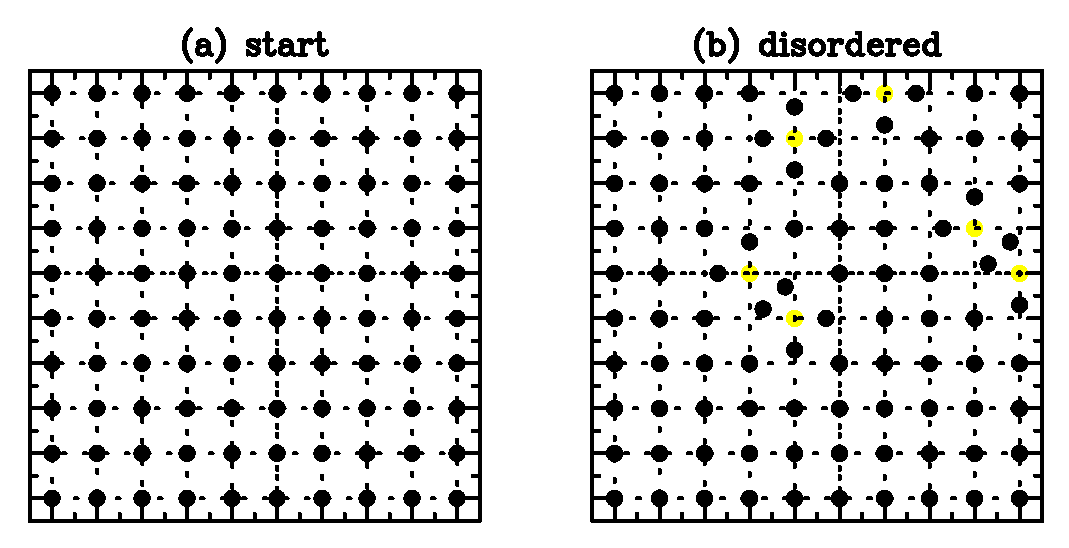
\includegraphics[scale=0.9, angle=0]{mod1.1.eps}
   \caption{Structures created by crystal modification example}
   \label{mod1-fig1}
\end{figure}
%
Here is the macro used to create the described defects.  Again the
line numbers are only shown for convenience and not part of the
macro itself. To achieve a high degree of flexibility values like
crystal size or the number of defects to be created are stored in
variables at the beginning of the macro.  The desired crystal size
is stores in variables i[1], i[2] and i[3] (lines 1-3).  The
variable i[4] (line 5) gives the number of defects to be created
and r[1] (line 6) specifies the relaxation (here 30 \%) of the
surrounding neighbors towards the vacant site.
%
\begin{MacVerbatim}
     1  i[1] = 10
     2  i[2] = 10
     3  i[3] = 1
     4  #
     5  i[4] = 6
     6  r[1] = 0.30
     7  #
\end{MacVerbatim}
%
Next we read the unit cell from file {\it cell.cll} and expand it to
the desired size (lines 8-9).  The macro {\it plot.mac} (line 11)
saves the starting structure suitable for plotting with {\it KUPLOT}
as seen in figure \ref{mod1-fig1}a).
%
\begin{MacVerbatim}
     8  read
     9  cell cell.cll,i[1],i[2],i[3]
    10  #
    11  @plot before.plot
    12  #
\end{MacVerbatim}
%
The next part (lines 13-15) is needed to switch off periodic crystal
boundaries for the command {\tt find} (line 24), otherwise our
simple way of relaxing the neighbors would not work.
%
\begin{MacVerbatim}
    13  chem
    14  set mode,quick,noperiodic
    15  exit
\end{MacVerbatim}
%
Now the creation of the disordered structure starts with a loop over
the number of defects to be created (line 19).  Next a crystal site
is chosen at random (line 20).  Note that the function {\tt ran(0)}
produces a random number between 0 and 1 which is multiplied with
the number of atoms within the crystal (n[3] contains the number of
atoms per unit cell, see table \ref{v1-tab} in section \ref{get}).  
If an occupied site
was picked (line 22) the atom is removed (line 23).  The command
{\tt find} (line 24) returns all atoms of the type Zr around the
position of the selected site within a radius of 5.5\AA.  The atom
indices of these nearest neighbors are stored in the variables {\tt
env[$<$i$>$]} and {\tt env[0]} contains the number of found
neighbors. Finally the positions of all neighboring atoms returned
by {\tt find} are moved towards the vacant site (lines 27-29).
%
\begin{MacVerbatim}
    16  #
    17  # Loop number of wanted defects
    18  #
    19  do i[5]=1,i[4]
    20    i[6]=int(ran(0)*i[1]*i[2]*i[3]*n[3])+1
    21  #
    22    if(m[i[6]].eq.1) then
    23      m[i[6]]=0
    24      find env,zr,x[i[6]],y[i[6]],z[i[6]],5.5
    25  #
    26      do i[7]=1,env[0]
    27        x[env[i[7]]]=x[env[i[7]]]-r[1]*(x[env[i[7]]]-x[i[6]])
    28        y[env[i[7]]]=y[env[i[7]]]-r[1]*(y[env[i[7]]]-y[i[6]])
    29        z[env[i[7]]]=z[env[i[7]]]-r[1]*(z[env[i[7]]]-z[i[6]])
    30      enddo
    31  #
    32    endif
    33  #
    34  enddo
    35  #
    36  @plot after.plot
\end{MacVerbatim}
%
The resulting structure can be seen in figure \ref{mod1-fig1}b.
The introduced vacancies are shown as yellow circles (or light
grey). Since this simple macro does not check whether neighboring
atoms are already displaced, the clustered defects in the upper
right quadrant of figure \ref{mod1-fig1}b have a different local
environment compared to the isolated defects.

%------------------------------------------------------------------------

\section{Build in functions \label{mod-buildin}}

This section will give an overview of those \Discus functions
modifying single atoms or molecules.  Some of these functions can be
realized using variables as well, others cannot like the command
{\tt insert} to insert a new atom in the model crystal.  Table
\ref{mod-tab-1} summarizes the available commands.
%
\begin{table}[!tbh]
\centering
\begin{tabularx}{\textwidth}{|p{30mm}|X|}
  \hline
  {\bf Command} & {\bf Description} \\
  \hline\hline
  append  & Appends an atom at a given position within the crystal if
            no other atoms are present in a given distance.\\
  copy    & Copies an atom to a different position given absolute or
            relative to the other position.\\
  insert  & Inserts a new atom at the given position without condition.\\
  kick    & Inserts a new atom at a given position and removes all
            other atoms within a given distance from the new atom.\\
  remove  & Removes an atom or molecule from the crystal.\\
  switch  & Swaps two given atoms or molecules within the crystal.\\
  purge   & Removes vacancies (VOID) from the crystal ({\bf use with
            care})\\
  replace & Replaces one or more atoms or molecules with the given
            type.\\
  \hline
\end{tabularx}
\caption{\label{mod-tab-1}\Discus commands for single atoms or
         molecules}
\end{table}
%
Basically there are three commands to insert a new atom in the
structure. The command {\tt insert} just creates a new atom at a
specified position without taking notice of its environment. Thus
the new atom might be on top of an existing one. In order to avoid
this problem, \Discus provides two other commands {\tt append}
which will not insert the atom if there are other atoms within a
given distance and {\tt kick} which will remove those atoms close by
before inserting the new one. The command {\tt copy} allows the user
to copy an existing atom to a new position that can be given in
absolute coordinated or relative to the position of the atom to be
copied. Note, that these commands are limited to atoms. New molecule
types can be created and molecules copied using the generalized
symmetry segment of \Discus described in chapter
\ref{cryst-sym}. \par

The commands {\tt remove} and {\tt switch} work for atoms as well as
molecules. Not surprisingly, {\tt remove} removes an atom or
molecule and {\tt switch} swaps two atoms or molecules with respect
to their location within the crystal. \par

The commands mentioned in this section so far operate only on a
single atom or molecule. The command {\tt replace} can replace a
single atom or molecule by a given type or replace more until a
given concentration is reached. Although this can be easily realized
using the FORTRAN interpreter and variables associated with the
crystal, the internal function is much faster, especially for large
crystal sizes. The command {\tt purge} will remove all vacancies
(VOID) within the crystal. Note that if you remove an atom or a
molecule by the {\tt remove} command, \Discus will not actually
remove atoms but rather replace their atom type with VOID. Thus when
saving the structure a large number of VOID's might appear in the
number. The use of {\tt purge} actually removes those VOID atoms.
However, the use of the {\tt purge} command is {\bf not recommended}
since many \Discus function require the crystal to be build in
a given order, i.e. having the same number of atom sites within
every unit cell either occupied by an atom or a VOID.

%------------------------------------------------------------------------

\section{Inserting extended objects \label{mod-insert}}

In order to insert extended objects for small angle scattering or
domains \ref{mod-domain} \Discus offers an insert menu. In contrast
to the insert command for individual atoms, the menu is evoked by
the {\tt insert} command followed by the keyword {\tt domain} or
{\tt object}. A corresponding version for molecules is under
construction. 

\subsection{Inserting domains \label{mod-insdom}}

Within the \Discus formalism, a domain (see section 
\ref{mod-domain} for a full explanation ) is 
essentially a molecule which will be interpreted differently. 
The domain allows you to place an extended defect into a host 
structure. The {\tt insert domain} menu allows you to specify
the character and location of the domain to be inserted.
%------------------------------------------------------------------------

%------------------------------------------------------------------------
% Chapter:  Build in defect models
%------------------------------------------------------------------------

\chapter{Build in defect models \label{mod}}

The following built in defect models modify the whole structure.
They offer extended defects that include modification of many
atoms throughout the whole crystal.  While such modifications
could be achieved as well by the user through extended use of the
FORTRAN interpreter, this would require extremely lengthy and
necessarily slow macros.  Defect models built in the source code
of the program on the other hand are calculated in much shorter
time.  The defect models were implemented with as many general
features as seemed necessary.  They use separate sub menus to
define the intended defect structure.

%------------------------------------------------------------------------

\section{Thermal displacements \label{mod-therm}}

The command {\tt therm} can be used to randomly displace all atoms
or rigid molecules of the crystal as to be expected by purely random
thermal disorder.  The direction of the displacement is distributed
with a uniform random spherical distribution.  The amplitude of the
displacement is distributed by a Gaussian distribution.  The mean of
the distribution is zero, its sigma is calculated from the isotropic
thermal coefficient, B, of each atom as:
%
\begin{equation}
    \langle u^{2} \rangle = \frac{B}{8 \pi^{2}}
    \label{therm-eq1}
\end{equation}
%
After the command {\tt therm} is executed, a summary of theoretical
and achieved displacement averages is displayed on the screen. An
example is shown below:
%

\begin{MacVerbatim}
   Thermal displacements summary :

                 Input               Achieved             Maximum displacement
   Atom        B   <u**2>     <ux**2> <uy**2> <uz**2>        x      y      z
   ---------------------------------------------------------------------------
   LA(1)     0.34  0.0043      0.0043  0.0043  0.0044     0.2299 0.2450 0.2487
   MN(2)     0.21  0.0027      0.0027  0.0027  0.0026     0.1980 0.1868 0.2184
   O(3)      0.50  0.0063      0.0061  0.0063  0.0064     0.2827 0.3518 0.3011
   O(4)      0.43  0.0054      0.0054  0.0055  0.0055     0.2745 0.3036 0.2855
\end{MacVerbatim}
%
The first column lists the name of the atom type followed by the B
and corresponding $\langle u^{2} \rangle$ value. The next three
columns show the achieved $\langle u_{i}^{2} \rangle$ values for
the x-, y- and z-direction. The last three columns give the
maximum displacements in the three directions that were
introduced. The values are given in \AA$^{2}$ and \AA. \par

The parameter {\tt mol} will displace rigid molecules according to
the B value of the atom at the origin of the molecule. Furthermore
the parameter {\tt 2d} allows to restrict the displacements to
directions with more than one unit cell extension of the crystal.
This might be used when working with 2-dimensional model crystals
where a displacement in the third direction is not wanted.

%------------------------------------------------------------------------

\section{Modulations \label{mod-wave}}

The given structure can be modulated using the {\tt wave} segment of
the program \Discus. Three different types of waves are
available, density waves modulating the occupation of sites within
the crystal, displacements waves modulating the position of atoms or
molecules and rotational waves which modulate the orientation of
molecules by rotating them around a user defined axis. First common
features shall be described followed by details about the different
wave types in separate sections. \par

\Discus offers three different wave functions $w({\bf r})$,
sinusoidal, square and saw tooth defined in equations
\ref{wave-eq1}, \ref{wave-eq2} and \ref{wave-eq3}, respectively. The
parameter $\delta$ for the box shaped wave functions determines its
asymmetry. The symmetric case is given by $\delta = 0.5$. The
computed value of $w({\bf r})$ modulates density, position or
orientation as a function of the position ${\bf r}$ within the
crystal depending on the wave type selected.
%
\begin{eqnarray}
    w({\bf r}) & = & A \cos (2\pi\left [
                    \frac{{\bf kr}}{\lambda}+\psi\right ]) + A_{0}
    \label{wave-eq1}  \\
    w({\bf r}) & = & \left \{
       \begin{array}{ll}
       A+A_{0} & \mbox{for $\frac{\delta}{2} \leq
                            \left | \frac{\bf kr}{\lambda}+
                                \frac{\psi}{360^\circ} \right | <
                            1 - \frac{\delta}{2}$}\\
       A_{0}   & \mbox{otherwise}\\
       \end{array} \right.
    \label{wave-eq2}  \\
    w({\bf r}) & = & A \left [\frac{{\bf kr}}{\lambda}+
                                  \frac{\psi}{360^\circ} \right ] + A_{0}
    \label{wave-eq3}
\end{eqnarray}
%
The following list describes the different properties common to all
wave types that can be defined by the user.
%
\begin{itemize}
    \item  {\it Wave vector ${\bf k}$:}
    The wave vector ${\bf k}$ defines the {\it traveling} direction of the wave.
    The vector is defined using the {\tt vect} command in multiples of the base
    vectors of the crystal, i.e.  in unit cell units.

    \item  {\it Wave length $\lambda$:}
    The wave length $\lambda$ of the modulation wave is entered using
    the {\tt len} command. Note that $\lambda$ must be given in \AA.

    \item  {\it Amplitude $A$:}
    The amplitude $A$ defines the upper limit of displacements (in \AA) or
    rotation angle (in degrees). In case of density waves the probability
    of replacing an atom or molecule oscillates between an upper and
    lower limit (see section \ref{mod-wave-dens}). The command to set the
    amplitude $A$ is {\tt amp}.

    \item  {\it Constant offset $A_{0}$:}
    A constant displacement or rotation angle can be added to all
    selected atoms or molecules using the command {\tt amp0}.

    \item  {\it Phase $\psi$:}
    The phase $\psi$ of the atom or molecule at (0,0,0) can be altered via the
    command {\tt phase}.
\end{itemize}
%
The argument $[{\bf kr} / \lambda +\psi / 360^\circ]$ of the wave
functions is limited to the range of -1 to 1 for the box and saw
tooth function and to a range of $\pm 2 \pi$ for the sinusoidal wave
function.  The origin of the vector ${\bf r}$ is the crystals
origin.  \Discus allows the user to select which of the atoms
in the crystal are to be modified by the wave function.

\subsection*{Density waves \label{mod-wave-dens}}

Displacement waves are selected using the {\tt dens} command.  A
density wave replaces an existing atom or molecule by another atom
or molecule type or alternatively removes the atom or molecule. The
direction of the density wave is along the wave vector. A lower and
upper probability $P_{low}$ and $P_{high}$ for replacing an atom or
molecule must be provided using the command {\tt plow} and {\tt
phigh}. The probability for the current atom or molecule to remain
in the structure oscillates between these two values. The
parameters $A$ and $A_{0}$ are calculated from these two
probabilities. In case of a sinusoidal wave the parameters $A$ and
$A_{0}$ are defined by:
%
\begin{eqnarray}
    A     & = & \frac{1}{2} ( P_{high} - P_{low})
    \nonumber \\
    A_{0} & = & \frac{1}{2} ( P_{high} + P_{low})
    \label{wave-eq4}
\end{eqnarray}
%
In case of a box or saw tooth shaped wave function, the parameters
$A$ and $A_{0}$ are determined by the following equations:
%
\begin{eqnarray}
    A     & = & P_{high} - P_{low}
    \nonumber \\
    A_{0} & = & P_{low}
    \label{wave-eq4b}
\end{eqnarray}
%
A random number is calculated every time an atom is encountered
that had been selected.  If this random number is less than
$w({\bf r})$, the amplitude calculated by the wave function, the
atom or molecule is retained as was, otherwise it is deleted or
replaced by another atom or molecule. Its position is not changed.

\subsection*{Displacement waves \label{mod-wave-disp}}

Displacement waves are selected using the {\tt trans} command.  For
displacement waves, the wave function $w({\bf r})$ determines the
displacement of an atom or molecule along a given direction of
oscillation. The command {\tt osci} defines the oscillation
direction in lattice units. \Discus allows any direction of
that vector relative to the propagation direction of the wave.  In
cases where propagation and oscillation vector are parallel, we
speak of longitudinal waves. In cases where propagation and
oscillation are normal to each other we speak of a transversal wave.
\par

The default displacement mode is set to acoustic, i.e.  all atoms
are displaced in the same direction.  An (admittedly crude) optical
mode will displace all atoms that are identified as negative ions in
the opposite direction to all others.  Negative ions are recognized
through their respective name, e.g. {\tt CL1-}. As a side effect, if
charged ions are used, the Fourier transform will use the
corresponding scattering curve.  If this is to be avoided, calculate
the desired wave twice, once with positive amplitude and once with
negative, while selecting the corresponding atoms.

\subsection*{Rotational waves \label{mod-wave-rot}}

Another feature of \Discus are rotational waves limited to be
used with molecules.  Obviously rotating an atom around itself makes
no sense. Rotational wave are selected with the {\tt rot} command
followed by parameters defining the rotation axis relative to the
molecules origin in lattice units.  The wave function $w({\bf r})$
then modulates the rotation angle ${\phi}$ around this axis.
Additionally an optional offset relative to the molecule origin for
the rotation axis can be specified by the {\tt rot} command.
%
\begin{figure}[!tbh]
   \centering
   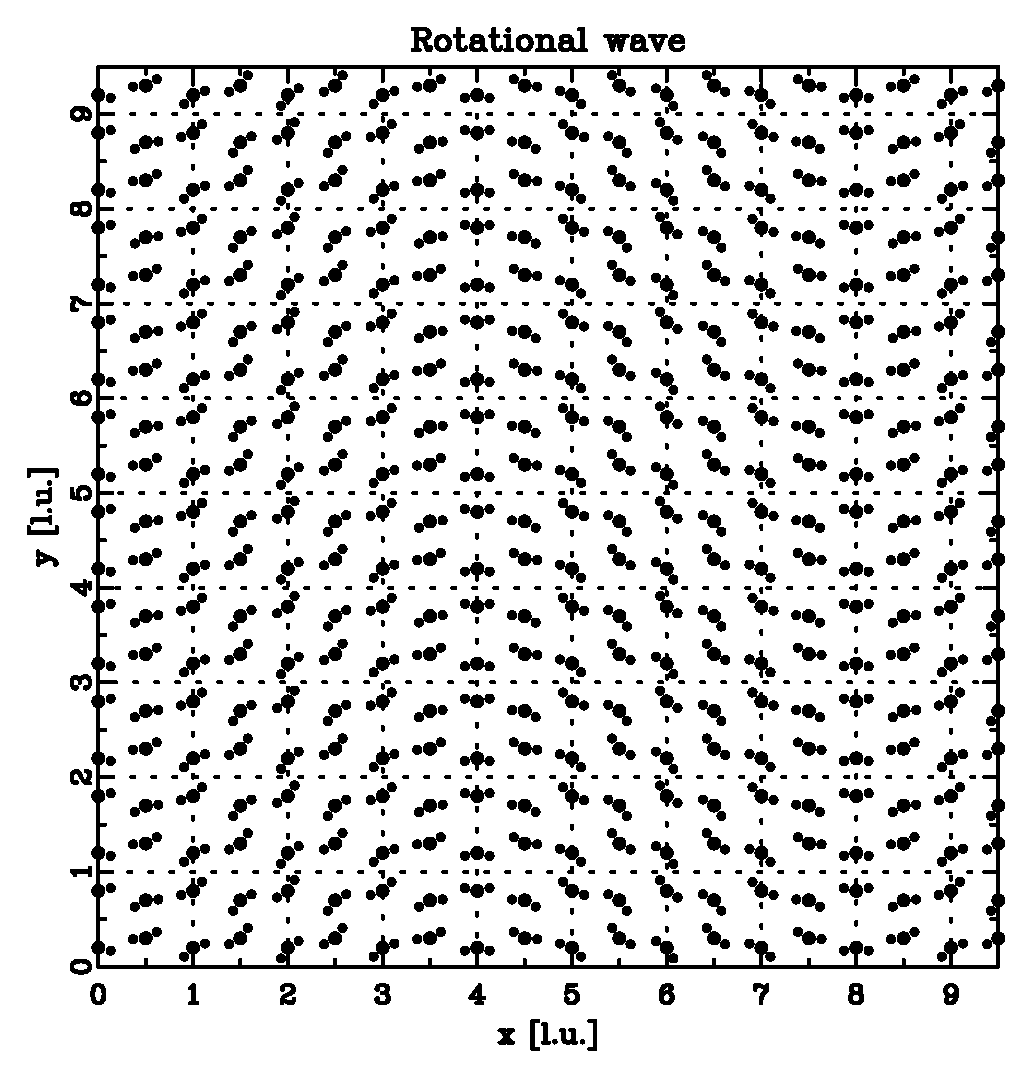
\includegraphics[scale=0.50, angle=0]{wave.3.eps}
   \caption{Example of a rotational wave}
   \label{wave-fig3}
\end{figure}
%
An example of such a rotational wave can be seen in figure
\ref{wave-fig3}. Here a cubic crystal with a size of 20x20x1 unit
cells (a = 10\AA) was used, each containing four $H_{2}O$ molecules.
The rotation axis is normal to the drawing plane, i.e. in
z-direction.  The wave vector is parallel to x and the wave length
$\lambda$ is eight unit cells (80 \AA).  The amplitude $A$ was set
to 45.0, i.e.  the rotation angle $\phi$ oscillates between $\pm 45$
degrees. \par

%------------------------------------------------------------------------

\section{Domains \label{mod-domain}}

The {\tt domain} module of \Discus has replaced the microdomain
module. A domain within \Discus is understood as a place holder
for an extended defect. This defect might be as small as an 
individual atom or be a region that extends over many unit cells.
 
Note, that in our book \citep{nedpro} we present examples using 
this domain module  and discuss domains at length. \par

As usual, the commands related to this modules are accessed after
entering the module via the command {\tt domain}. Let us look at a
simple example how to use this module:
%
\begin{MacVerbatim}
   1  domain
   2    rese
   3    mode   pseudo
   4    input  dom.cube.pseudo
   5    assign char,si,sphere
   6    assign fuzzy,si,0.5
   7    assign cont, si,dom.guest.cube.stru
   8    assign shape ,si,1,  1. , 0. , 0. ,  0.
   9    assign shape ,si,2,  0. , 1. , 0. ,  0.
  10    assign shape ,si,3,  0. , 0. , 1. ,  0.
  11    assign orient,si,1,  1. , 0. , 0. ,  0.
  12    assign orient,si,2,  0. , 1. , 0. ,  0.
  13    assign orient,si,3,  0. , 0. , 1. ,  0.
  14    show
  15    run
  16  exit
\end{MacVerbatim}
%
After resetting the module (line 2), mode {\tt pseudo} is selected.
In this mode, a \Discus structure file is used to define the
distribution of domains and each {\it pseudo atom} in this file is
later replaced by the corresponding domain. In our case, the atom Si
is replaced by the defined spherical domain (line 5). The boundary
is created by removing all atoms that are within 0.5\AA\ of the
domain (line 6). Next the domain dimension is define using the
matrix defined in lines 8--10. These values are in terms of unit
cells of the host structure. The second matrix (lines 11-13) defines
the orientation of the domain. Finally the settings are listed (line
14) and the domain is finally created (line 15). There is an
alternative extension of a structure file and the keyword {\tt
domain} allows to readily define the domain structure, its shape and
orientation (see \citet{nedpro}).
\par

%------------------------------------------------------------------------

\section{Stacking faults \label{mod-stack}}

All crystals whose structures can be described by layers are prone
to stacking faults.  A stacking fault is any defect that alters the
periodic sequence of layers.  These defects may be a wrong layer
inserted into the sequence, a change of the layer sequence or a
different translation between two subsequent layers.  These defects
may affect the whole crystal or a finite region if e.g. an
additional layer is present between an otherwise perfect sequence of
layers.  \Discus contains a tool to create layered crystal
structures and to introduce stacking faults into these crystals. The
crystals are formed in a two step procedure. First, the origin and
type of each layer is determined and second, the atoms corresponding
to each layer are introduced into the crystal.  The user can define
each layer type, the translation vectors between consecutive layers
and the correlation between neighboring layers. A new feature of the
stacking fault part of \Discus is the addition of rotational
disorder for the layer sequences. \par

The stacking fault sequence is defined by several parameters that
can be set in the {\tt stack} sub level of \discus:
%
\begin{itemize}
    \item  {\it Type of layers :}
    The positions of all atoms within a layer are read from a \Discus type
    structure file.  These layer files have to be created for each layer type
    involved beforehand using the various \Discus tools.

    \item  {\it Translations :}
    A translation vector between neighboring layers of each type must be
    provided.  Thus N different layer types result in a N*N matrix of
    translation vectors.  An example for translation vectors in a cubic face
    centered structure is given in table \ref{mod-stack-tab1}.

    \item  {\it Uncertainties for translation vectors:}
    In some materials small deviations in the translation vectors might occur.
    This behavior can be simulated in \Discus by setting a standard
    deviation $\sigma$ to each of the elements of the translation vector
    matrix.  \Discus will calculate the actual translation vector as sum
    of the 'ideal' vector plus a Gaussian distributed part defined by the value
    of $\sigma$.

    \item  {\it Correlations :}
    A correlation matrix is used to define the probabilities of two layer types
    to be nearest neighbors.  No further correlations are taken into account.
    To create correlations with {\it Reichweite} larger than 1, you can build 
    a one dimensional crystal of two or more atom types. The types and positions
    of these atoms can be interpreted as layer types and origins.

    \item  {\it Crystal shape :}
    The resulting crystal can be generated using two different modes: First,
    the crystal continuously grows in one direction as given by the translation
    vector(s).  Secondly one or two coordinates can be constrained to a finite
    range, which results in a zig-zag shaped crystal.  If any of the parameters
    is not equal to zero, the corresponding coordinate of the origin is taken
    modulo this parameter.  Note, that \Discus does not check whether the
    modulo vectors are translation vectors of the current space group.
\end{itemize}
%
\begin{table}[!tbh]
\centering
\begin{tabular}{|c|c|c|}
  \hline
  {\bf Layer type A} & {\bf Layer type B} & {\bf Translation vector} \\
  \hline\hline
  A & A & $(1, 1, 1)$ \\
  A & B & $\frac{1}{2} (1,1,0)$\\
  A & C & $\frac{1}{2} (1,0,1)$\\
  B & A & $\frac{1}{2} (\overline{1},\overline{1},0)$\\
  B & B & $(1, 1, 1)$\\
  B & C & $\frac{1}{2} (0,1,1)$\\
  C & A & $\frac{1}{2} (\overline{1},0,\overline{1})$\\
  C & B & $\frac{1}{2} (0,\overline{1},\overline{1})$\\
  C & C & $(1, 1, 1)$\\
  \hline
\end{tabular}
\caption{\label{mod-stack-tab1}Translation vectors for stacking
         faults in a cubic face centered structure}
\end{table}
%
The command {\tt create} in the {\tt stack} segment of \Discus
creates the list of layer origins and {\tt run} actually generates
the corresponding crystal by decorating the origins with the
individual layer types.  In order to speed up the calculation of the
Fourier transform, rather than using the resulting complete
structure, the scattering intensity is calculated in the following
way.  The scattering density $\rho ({\bf r})$ of a layered structure
can be expressed as the scattering density of the individual layer
types convoluted with the layer origin distribution.
%
\begin{equation}
    \rho({\bf r}) = \sum_{i=1}^{nl} \left \{ \sum_{j=1}^{no}
                    o_{ij} ({\bf r}) \right \} \star l_{i} ({\bf r})
    \label{mod-stack-eq1}
\end{equation}
%
The outer sum runs over all $nl$ layer types and the inner sum
runs over all origins $o_{ij}$ of layer type $i$.  The variable
$l_{i}$ is the scattering density of layer type $i$.  Using the
convolution theorem, the Fourier transform of this expression
becomes
%
\begin{equation}
    {\cal F} \left \{ \rho({\bf r}) \right \} =
        \sum_{i=1}^{nl}
              {\cal F} \left \{ \sum_{j=1}^{no} o_{ij} ({\bf r}) \right \}
        \cdot {\cal F} \{ l_{i} ({\bf r}) \}
    \label{mod-stack-eq2}
\end{equation}
%
Here ${\cal F}$ denotes the Fourier transform.  This procedure not
only speeds up the calculation but it also allows the usage of much
larger crystal sizes since the actual structure does not have to be
created in order to calculate the Fourier transform.
\par

%------------------------------------------------------------------------

\section{Surfaces \label{mod-surface}}

An initial model crystal will be a block of IxJxK unit cells. This shape
is ideal to avoid finite size effects when you want to calculate diffuse
scattering for an infinite large crystal. Nanoparticles or domains are
of course explicitly finite objects, whose shape you might want to 
control. \Discus offers the {\tt surface menu} to shape the crystal into
a finite sized object. The menu replaces the {\tt boundary} command that
is still available for backward compatibility.

Within the {\tt surface} menu, the {\tt boundary} command allows you to
shape the crystal by any combination of:\\
\begin{itemize}
\item an individual lattice plane {\tt HKL}
\item a form, i.e. a set of symmetrically equivalent lattice planes {\tt HKL}
\item a spherical surface
\item a triaxial ellipsoidal surface
\item a cylindrical surface
\end{itemize}

A plane will remove all atoms to one side of this plane:

\begin{MacVerbatim}
boundary hkl, 1, 1, -1, 15.0, inside
\end{MacVerbatim}

In this example a 11$\overline{1}$ plane is placed at 15.0\AA from the 
origin. All
atoms remain that are inside the boundary plane i.e. at the same side 
of the plane as is the origin 0.0, 0.0, 0.0. As a plane extends to 
infinity parallel to its surface, \Discus cannot create an object with
an indented surface using individual planes. 
Such an object can be build using a {\\tt form}, {\\tt sphere}, 
{\\tt ellipsoid} or {\\tt cylinder}.

A complete form of symmetrically equivalent faces can be created via:

\begin{MacVerbatim}
boundary form, 1, 1,  1, 15.0, inside
\end{MacVerbatim}

This will create an object that is limited by the complete set of
all symmetrically equivalent \{111\} faces. Keep in mind that this
set of faces will depend on the point group symmetry of your crystal!

A spherical object with radius R is created by the command:

\begin{MacVerbatim}
boundary sphere, 35.0, inside
\end{MacVerbatim}

A triaxial ellipsoid with diameters DX=20, DY=30, DZ=40 \AA\  is 
created by the command:

\begin{MacVerbatim}
boundary ellipsoid, 20, 30,40, inside
\end{MacVerbatim}

Admittedly it is a bit of an inconsistency that the "ellipsoidal" surface 
takes diameters instead of radii. Independent of the crystal system,
the three axes of the ellipsoid are always orthogonal to each other. 
The ellipsoid is oriented in a standard fashion. This orientation
is chosen such that the ellipsoid "Y"-axis is parallel to the 
crystallographic b-axis, the "Z" axis parallel to the c$*$ axis
and the "X" axis  forms a right handed orthogonal system. Table
\ref{mod-surf-tab1} lists the resulting orientations for the seven crystal systems:

\begin{table}[!tbh]
\centering
\begin{tabular}{|c|r|c|l|}
  \hline
  {\bf system} & {\bf X-axis} & {\bf Y-axis } & {\bf Z-axis} \\
  \hline\hline
  cubic        & {$\vec{a}$} = [100]                   & {$\vec{b}$} = [010]& {$\vec{c}$} = [001] \\
  hexagonal    & {$\vec{a^{*}}$} = [210]               & {$\vec{b}$} = [010]& {$\vec{c}$} = [001] \\
  trigonal     & {$\vec{a^{*}}$} = [210]               & {$\vec{b}$} = [010]& {$\vec{c}$} = [001] \\
  rhombohedral & {$\vec{b}\otimes\vec{c^{*}}$}         & {$\vec{b}$} = [010]& {$\vec{c^{*}}$}     \\
  tetragonal   & {$\vec{a}$} = [100]                   & {$\vec{b}$} = [010]& {$\vec{c}$} = [001] \\
  orthorhombic & {$\vec{a}$} = [100]                   & {$\vec{b}$} = [010]& {$\vec{c}$} = [001] \\
  monoclinic   & {$\vec{b}\otimes\vec{c^{*}}$} = [100] & {$\vec{b}$} = [010]& {$\vec{c^{*}}$}     \\
  triclinic    & {$\vec{b}\otimes\vec{c^{*}}$} = [100] & {$\vec{b}$} = [010]& {$\vec{c^{*}}$}     \\
  \hline
\end{tabular}
\caption{\label{mod-surf-tab1}Orientation of an ellipsoidal 
surface for the seven crystal systems.}
\end{table}

If the last parameter on the {\tt boundary} command is {\tt outside},
all those atoms are retained that are on the outside of the given
surface. For a single plane, only those atoms remain, that are on the 
outside of the surface. For the closed shapes {\tt form}, 
{\tt sphere}, {\tt ellipsoid}, {\tt cylinder} a cavity inside your
crystal will be the result. Keep in mind, that the {\tt form} will
not necessarily result in a true closed shape. Whether a closed
shape results depends on the actual Miller indices and the point 
group.


In order to create closed interior hollow spaces in low-symmetry 
structures, the shapes: {\tt sphere}, {\tt ellipsoid}, {\tt cylinder}
can be used in any crystal system. If the shape shall consist 
of flat surfaces you will likely need a combination of several
symmetrically non-equivalent faces to generate a closed shape.
\Discus provides optional parameters to the {\tt boundary command}
 for this  purpose:

\begin{MacVerbatim}
boundary  form, 1, 0,  1, 15.0,outside, accum:init, exec:hold
boundary  form, 1, 0, -1, 15.0,outside, accum:add , exec:hold
boundary  hkl , 0, 1,  0, 15.0,outside, accum:add , exec:hold
boundary  hkl , 0,-1,  0, 15.0,outside, accum:add , exec:run
\end{MacVerbatim}

The "accum:init" indicates to \Discus to initialize a list of
faces/forms. The actual cut is put on hold via the 
"exec:hold" statement. the next two commands add a further face
to the collection, while still keeping the execution on hold. 
The third statement finally adds the last face to make a 
completely closed shape in point group P2. As this is the final 
faces, the execution is performed via the "exec:run" parameter.

To shape an convex object, these two optional parameters are 
not needed, as each face may cut away the atoms independently.
For that reason, the two parameters default to
"accum:init" and "exec:run". 

Three further optional parameters allow you to place the center of the 
shape at an arbitrary point. These parameters take the style:

\begin{MacVerbatim}
boundary form, 1, 1,  1, 15.0, inside, centx:1.0, centy:2.0, centz:3.0
\end{MacVerbatim}

The colon ":" indicates that this is an optional parameter. The
value after the colon defines the respective position of the 
center along the three crystallographic axes. All values default
to zero.


%------------------------------------------------------------------------

\section{Decorating Surfaces \label{mod-deco}}

The {\tt decoration} menu within \Discus can be used to decorate
a surface with a group of additional atoms. The steps involved in such
a decoration process are two fold:
\begin{itemize}
\item Shape a crystal into the desired form via the {\tt surface} menu
\item Place one or several ligand molecules onto the surface
\end{itemize}

A common set of command to achieve this would be:
\begin{MacVerbatim}
 1  read
 2     cell structure.cell, 20, 20, 20
 3  surface
 4     boundary form, 1,0,0, lat[1]*4.5, keep:inside
 5  exit
 6  #
 7  decorate
 8     reset
 9     add example, normal
10     set example, ligand, ligand.stru, 0.015
11     set example, bond,   au, 1, 2.42
12     set example, axis, auto
13     set example, form,  1, 0, 0
14     show
15     run
16  exit
\end{MacVerbatim}

After the shaping of the crystal into a cube (here assuming a cubic 
structure in "structure.cell") \Discus enters the {\tt decorate} menu
in line 7. Once the mode is reset to ensure clean starting conditions,
a new decoration mode is {\tt added} in line 9. The string "example"
serves as a name for further references. The bonding style for this
decoration scheme is set to {\tt normal}. This will place the ligand
molecule with a single bond onto the surface and align the molecule
normal to the local surface. \Discus currently offers six bonding
schemes that are detailed further down. In line 10 we specify the
source of the decorating molecule as the file {\tt ligand.stru}. 
The molecule shall be placed onto the surface at a (rough) density of 
0.015 molecules per \AA$^2$. Line 11 specifies that a 
single bond between surface "Au" atoms and the first atom in 
ligand.stru should be build at a bond distance of 2.42\AA. \Discus is 
instructed in line 12 to align the molecule axis automatically.
Finally in line 13 the decoration is limited to surfaces that 
belong to the form \{100\} of the current crystal system. The 
standard {\tt show} and {\tt run} commands complete the action.

After this quick run through a more detailed explanation will follow. 
\Discus
will place the molecule contained in the file specified on the
{\tt ligand} instruction onto the surface of the particles. Prior
to this placement process, the particle must have been shaped via the 
{\tt surface} menu as \Discus relies on the surface property that is
generated in the {\tt surface} menu. Once you have chosen surface 
atoms onto which the guest molecules shall be placed, \Discus will
internally select these surface atoms and arrange these as evenly as 
possible on the surface. This distribution process attempts to
avoid overlap between the individual guest molecules. Admittedly 
this will not always be perfect, especially for a high surface 
density. If necessary use a lower density or use the {\tt mmc} 
menu to twist the guest molecules in order to avoid an overlap.

Currently \Discus offers six different bonding schemes for the 
nanoparticle decoration:
\begin{itemize}
\item {\tt normal} The molecule is placed with a single bond onto the
      surface. This bond is oriented normally to the local surface
      on top of the surface atom.
      Either automatically or via the pair of atoms provided via the
      {\tt axis} keyword, \Discus aligns the molecule itself normal
      the the surface as well.
\item {\tt bridge} The molecule is placed with two bonds onto the
      surface, midway between the two surface atoms. Both bonds 
      have the same length and an equilateral triangle results. 
      The plane of this triangle is placed parallel to the local 
      surface normal.
      The remainder of the molecule is 
      aligned as in the {\tt normal} mode.
\item {\tt double} The molecule is placed with two bonds onto the
      surface. In contrast to the {\tt bridge} mode, two separate
      atoms from the ligand form respective bonds to two separate 
      surface atoms. Since the two bond may have different lengths, 
      the four atoms form a general quadrilateral. \Discus attempts
      to place the vector between the two molecule atoms parallel
      The plane of this quadrilateral is placed parallel to the local 
      surface normal.
      to the vector between the two surface atoms.
      The remainder of the molecule is 
      aligned as in the {\tt normal} mode.
\item {\tt multi} The molecule is placed with bonds between two
      molecule atoms to surface atoms. The first molecule atom
      builds two or more bonds of equal length to the corresponding
      number of surface atoms. The second molecule atoms forms a
      further single bond to a surface atom. The first atom is thus 
      in a generalized bridge position atop of the surface atoms. 
      If the surface group consists of four or more atoms, it will
      usually be impossible to obtain equal distances between the 
      molecule atom and all surface atoms. \Discus attempts to 
      place the atoms with as similar bonds as possible. Once the
      first molecule atom is placed, \Discus rotates the molecule
      to place the second molecule atoms into a position such 
      that it forms a single bond of specified length.
      The remainder of the molecule is 
      aligned as in the {\tt normal} mode.
\item {\tt acceptor} This mode serves to build a hydrogen bond 
      between a surface acceptor and a ligand molecule. 
      The user can specify the distance between the 
      surface acceptor atom and the "Hydrogen" atom in the molecule.
      This distance should of course be around 1.9\AA. This
      Hydrogen bond is placed normally to the local surface. \Discus 
      does not check if the atom in the molecule is actually a 
      Hydrogen atom, this responsibility is left to the user.
      As default \Discus rotates the molecule to achieve a 170$^\circ$
      bond angle in the Hydrogen atom.
      The remainder of the molecule is 
      aligned as in the {\tt normal} mode. In addition, the molecule
      is rotated by a random angle around the hydrogen bond.
\item {\tt donor} This counterpart to the {\tt acceptor} model 
      places the first molecule atom at the user specified hydrogen
      bond distance to the surface atom. Again, the distance should 
      be in the range of 1.9\AA\  and the surface atom should be a 
      hydrogen bond. The molecule atom is placed such that the 
      bond angle in the surface Hydrogen atom is by default
      170$^\circ$.
      The remainder of the molecule is 
      aligned as in the {\tt normal} mode. In addition, the molecule
      is rotated by a random angle around the covalent bond between 
      the surface hydrogen atom and its closest surface neighbor.
\end{itemize}

For each of these bonding schemes the user specifies the source of
the molecule. \Discus expects a standard structure file format as 
source. If your molecule resides in a {\tt CIF} file, please 
import this into the \Discus format first. The unit cell parameters
of the molecule do not have to be identical to those of the host
structure. \Discus will transform the coordinates internally.

For the bonding schemes {\tt acceptor} and {\tt donor} the 
hydrogen bond angle in the Hydrogen atoms defaults to 170$^\circ$.
To modify this angle \Discus provides the optional parameter
{\tt angle:value} to the {\tt set bond} command. 

\Discus will place the guest molecules at the user specified density 
(in molecules per square \AA ngstroem) onto the surface. This density
is roughly estimates using the number of surface atoms and assigning a
fixed area of 11\AA$^2$ to each surface atom. 

Depending on the bond scheme \Discus is left with freedom to align the complete
molecule. The schemes fix the position of the bonded molecule atoms only.
The remainder of the molecule is aligned roughly normal to the surface.
The user can specify a pair of atoms within the molecule or let \Discus
find the non-bonded molecule atom at furthest distance to the first
bonded molecule atom. Within the degrees of freedom of the bond scheme
the molecule is rotated to align the vector defined by these two atoms 
as close to the local surface normal as possible. For the {\tt normal}
, {\tt bridge} and {\tt donor} mode \Discus can freely rotated the 
molecule to achieve 
this orientation. For the {\tt double} and {\tt multiple} mode the 
molecule will be rotated around the vector between the two bonded molecule
atoms. As a result the molecule axis will be in the plane defined by the
surface atoms and the two bonded molecule atoms. This plane itself
is parallel to the surface normal. The molecule axis will be in this
plane but may still form an angle to the surface normal. For the
{\tt acceptor} mode, \Discus can rotate the molecule around the
Hydrogen-donor bond to align the molecule axis as close as possible to
the surface normal.

As default \Discus will place the guest molecule onto any surface atom type 
that occurs in any bond assignment. The user has the option to restrict
the placement onto an individual hkl plane or onto a form of symmetrically
equivalent planes. Thus, if you shaped the crystal into a polyhedron of
say the \{100\} and \{111\} faces, you have the option to restrict the 
placement onto either of the faces or forms.

When you use the {\tt boundary} command within the {\tt surface} menu to
shape the original crystal, \Discus will assign a surface property to 
those atoms that are close to the surface. Within the {\tt decorate} menu
\Discus uses this surface property to select atoms onto which a guest 
molecule can be placed. Thus it is mandatory to shape the crystal prior 
to any decoration. You may desire to build an initial crystal and to assign 
an external surface without actually removing any atoms. This might be
the case when you read a previously created structure that you want 
to decorate in a second step. In this case, you need to still "cut" 
the surface. In order not to remove any atoms, simply choose surfaces
parallel to the present surfaces and place these new surfaces just a little
bit outside the present surfaces. In combination with the 
{\tt set distance} command in the {\tt surface} menu atoms close to these
new surfaces will be flagged as surface atoms and can be used in the
decoration mode.

The atoms in the guest molecule receive a "Ligand" and a "Molecule" 
property, and these properties can be used for further manipulations.
The atoms do not automatically receive a surface property.
Currently \Discus does not try to decide which of the guest atoms are
at the "outside" in order to assign a correct surface property. It
appears the the molecule shape is too impredictable to do so fully
automatically. (\Discus may try to learn this in the future...)

The user can, however, assist by specifying guest molecule atoms 
that shall inherit the surface properties of the surface atom.
Use the command:

\begin{MacVerbatim}
set example, surface, atom_no
\end{MacVerbatim}
With this command, the listed atoms of the ligand molecule will 
receive the same surface properties as the original surface atom.
This will be useful, if you want to place a second layer of decorating 
molecules onto the surface.
%------------------------------------------------------------------------

%------------------------------------------------------------------------
% Chapter:  Analyzing defect structures
%------------------------------------------------------------------------

\chapter{Analyzing defect structures \label{chem}}

After describing how to create and change structures this chapter
will give a summary of \Discus functions to analyze a given
disordered structure. All those commands are accessed via the {\tt
chem} sub level of the program. This segment is entered using the
command {\tt chem} and left again by the command {\tt exit}. The
command {\tt mode} determines whether the entered commands operate
on atoms ({\tt mode atom}) or molecules ({\tt mode mole}). If
working with molecules the molecule type number replaces the atom
name or number as parameter for the different commands. Note that
not all commands are available in molecule mode. Also note, that the
\Discus cookbook \citep{nedpro} includes a complete chapter on
the analysis of disordered structures with many examples and
exercises.

These commands within the {\tt chem} menu allow a convenient way to 
analyze the whole structure. Individual atoms can be checked through
the general command language, see section \ref{chem-indiv}.
%------------------------------------------------------------------------

\section{Occupancies \label{chem-occ}}

The command {\tt elem} will display the chemistry of the current
model crystal. Depending on the selected mode the relative abundance
of the present atom or molecule types is written on the screen. The
results are saved in the variable {\tt res[i]} (see chapter
FORTRAN style interpreter in the package manual). Entry {\tt res[1]}
contains the relative amount of atom types {\tt void} and entries 
{\tt res[1]} the relative amount of atom type 1.

The relative abundances given by the command
{\tt elem} are for the complete crystal and contain no further
information about its homogeneity. \Discus allows the user to
obtain concentration as well as correlation (see section
\ref{chem-corr}) distributions within the crystal using the command
{\tt homo}. This is achieved by sampling the crystal using a
predefined volume.

%------------------------------------------------------------------------

\section{Distortions \label{chem-dist}}

After analyzing concentrations within a crystal, this section will
focus on the analysis of distortions. The simplest way is to compute
average distances between different atom types in a given range. An
example is given below. First the desired range of interatomic
distances is limited to values between 4.5\AA \ and 5.5\AA \ (line
1). Next the bond length distribution is calculated using the 
\Discus command {\tt blen}. Here distances between {\it all} atoms
will be considered and the resulting distribution is written to the
file {\it chem.2.blen} (line 2).
%

\begin{MacVerbatim}
     1  set blen,4.5,5.5
     2  blen all,all,chem.2.blen
\end{MacVerbatim}
%
Rather than using {\tt all} as parameters for the command {\tt
blen}, atom names or numbers could be used to calculate the average
bond length only for specify atom types.
\par

The command {\tt blen} averages {\bf all} distances within the given
range specified with {\tt set blen}. In cases where more specific
information about distances in given directions is needed, the
command {\tt disp} must be used. Now it is necessary to enter
neighbor definitions which can either be specified by a distance
criteria or by individual vectors. In the example below the command
{\tt set vec} in line 1 defines vector 1 (first 1) to be from site 1
in one unit cell to site 1 (2nd and 3rd parameter) in the next unit
cell in x-direction (1,0,0 - last 3 parameters). Next this vector is
used as neighbor definition 1 (line 2). Finally the lattice
averages are computed between all present atom types (line 3).
%
\begin{MacVerbatim}
     1  set vec,1,1,1,1,0,0
     2  set neig,vec,1
     3  disp all,all
\end{MacVerbatim}

%------------------------------------------------------------------------

\section{Correlations \label{chem-corr}}

In this chapter the concept of correlations as a measure for those
two-body interactions will be introduced. Although diffuse
scattering contains only information about two-body interactions the
concepts described here can easily be extended to include multi-site
correlations. It should be noted that although these multi-site
interactions do not show up in the diffraction pattern directly,
they can have a constraining influence on two-body interactions and
thus affect the diffraction pattern. However, \Discus is
currently limited to the calculation of two-body interaction
averages. \par

We will talk about atom types in the following section, however, all
correlation related commands are available for molecules as well. To
work with molecules use the command {\tt mode mole} and specify
molecule types rather than atom types or names as parameters for the
commands.

\subsection*{Occupational correlations \label{chem-corr-occ}}

One definition of the correlation coefficient $c_{ij}$ between a
pair of sites $i$ and $j$ based on a statistical definition of
correlation \citep{we85} is given in equation \ref{chem-eq1}.
%
\begin{equation}
    c_{ij} = \frac {P_{ij} - \theta^{2}} { \theta (1 - \theta)}
    \label{chem-eq1}
\end{equation}
%
$P_{ij}$ is the joint probability that both sites $i$ and $j$ are
occupied by the same atom type and $\theta$ is its overall
occupancy.  Negative values of $c_{ij}$ correspond to situations
where the two sites $i$ and $j$ tend to be occupied by {\it
different} atom types while positive values indicate that sites $i$
and $j$ tend to be occupied by the {\it same} atom type.  A
correlation value of zero describes a random distribution.  The
maximum negative value of $c_{ij}$ for a given concentration
$\theta$ is $-\theta/(1-\theta)$ ($P_{ij}=0$), the maximum positive
value is +1 ($P_{ij}=\theta$). Let us look at a simple example:
%
\begin{MacVerbatim}
     1  read
     2  stru chem.1.stru
     3  #
     4  chem
     5  #
     6    set mode,quick,periodic
     7  #
     8    set vec,1,1,1, 1, 0, 0
     9    set vec,2,1,1,-1, 0, 0
    10    set vec,3,1,1, 0, 1, 0
    11    set vec,4,1,1, 0,-1, 0
    12  #
    13    set vec,5,1,1, 1, 1, 0
    14    set vec,6,1,1,-1, 1, 0
    15    set vec,7,1,1, 1,-1, 0
    16    set vec,8,1,1,-1,-1, 0
    17  #
    18    set neig,vec,1,2,3,4
    19    set neig,add
    20    set neig,vec,5,6,7,8
    21  #
    22    corr occ,zr,void
    23  #
    24  exit
\end{MacVerbatim}
%
The macro starts with the reading of the disordered structure (lines
1-2). After the {\tt chem} sublevel is entered (line 4) periodic
crystal boundaries are selected (line 6).  The parameter {\tt quick}
selects a faster neighboring finding algorithm which only works for
crystals arranged in the \Discus storage order (see section
\ref{struc-int}).  Note that $c_{\langle 10 \rangle}$ stands for the
nearest neighbor correlations in all four symmetrically equivalent
$<$10$>$ directions of the two dimensional cubic test crystal, i.e.
$c_{10}$, $c_{\overline{1}0}$, $c_{01}$ and $c_{0 \overline{1}}$.
All eight neighboring directions for $c_{\langle 10 \rangle}$ and
$c_{\langle 11 \rangle}$ are defined as vectors 1 to 8 in lines 8 to
16 of the macro file.  Next vectors 1 to 4 are grouped as
neighboring definition for $c_{\langle 10 \rangle}$ (line 18) and
vectors 5 to 8 for $c_{\langle 11 \rangle}$ (line 20).  The command
'set neig,add' (line 19) stores the current neighboring definition
and allows the definition of a new one.  Finally the correlations
for the defined neighboring directions are calculated (line 22). The
screen output looks like this:
%
\begin{MacVerbatim}
    Calculating correlations
        Atom types : A = ZR   and B = VOID

        Neig.     AA         AB         BB         # pairs    correlation
        -----------------------------------------------------------------
           1    50.49 %    48.99 %      .51 %       40000       -.3061
           2    71.04 %     7.89 %    21.07 %       40000        .7897
\end{MacVerbatim}
%
The program lists the probabilities for AA, AB and BB pairs and the
corresponding correlations $c_{ij}$.  Here the value for $c_{\langle
10 \rangle}$ is negative, i.e.  vacancy neighbors in $<$10$>$
directions tend to be avoided.  Neighboring vacancies in $<$11$>$
direction on the other hand are much more likely compared to a
random vacancy distribution indicated by the large positive value of
$c_{\langle 11 \rangle}$.

\subsection*{Displacement correlations \label{chem-corr-disp}}

The correlation coefficient $c_{ij}$ for displacement correlations
between two sites $i$ and $j$ is defined as:
%
\begin{equation}
    c_{ij} = \frac { \langle x_{i} x_{j} \rangle }
                   { \sqrt { \langle x_{i}^{2} \rangle
                             \langle x_{j}^{2} \rangle } }
    \label{chem-eq2}
\end{equation}
%
Here $x_{i}$ is the displacement of the atom on site $i$ from the
average position in a given direction and $\langle \cdot \rangle$
stands for the average over the crystal.  Again a negative value
describes a situation where the pairing of corresponding
displacements are less likely than in a crystal with random
displacements whereas a positive value indicates a larger than
random probability. The definition of neighbors is identical to the
example in the previous section.  Additionally the command {\tt set
neig,dir} is used to determine the displacement direction to be
used. Note that the displacement direction for the two sites $i$ and
$j$ is not necessarily the same, e.g.  one could be interested in
the correlation between the x-displacement on one site and the
y-displacement on the neighboring site.

\subsection*{Correlation fields \label{chem-corr-field}}

In the previous sections a correlation $c_{ij}$ for a given pair of
neighboring atoms was computed. An interesting information, however,
is how these correlations extend within the crystal. The program
\Discus allows the calculation of correlation fields for
occupational and displacement correlations (command: {\tt field}).

%------------------------------------------------------------------------

\section{Bond valence sums \label{chem-bval}}

The concept of {\it bond valence} has found wide applicability in
solid state chemistry \citep{bral85,brok91}. One application is
the use of bond-valence sums at atoms as a check on the
reliability of a determined local structure. The valence of an
atom i is calculated by the following empirical expression:
%
\begin{equation}
  V_{i} = \sum_{ij} \exp \left\{ \frac{r^{0}_{ij} - d_{ij}}{b} \right\}
  \label{chem-eq-bval}
\end{equation}
%
Here $r^{0}_{ij}$ and $b$ are the so-called bond valence parameters,
$d_{ij}$ is the distance between the central atom i and the
neighboring atom j. The sum goes over all nearest neighbors. The
bond valence parameters used by \Discus were taken from a list
compiled by I.D. Brown, McMaster University, Hamilton, Canada from
various references. Those parameters can be displayed using the
command {\tt show}. An example is given below:
%
\begin{MacVerbatim}
    discus > show bval,zr4+,o2-
    Bond valence parameters ZR4+ - O2-  : r0 =  1.9280 b =  0.3700
\end{MacVerbatim}
%
The parameters are specific for a given atom pair, here Zr$^{4+}$
and O$^{2-}$. Note that it is required to use the atom names
indicating the oxidation state like in the example above. It should
also be noted, that bond valence parameters are not available for
all pairs of atoms.

%------------------------------------------------------------------------

\section{Other tools \label{chem-other}}

In this chapter a short summary of functions available in the 'chem'
sublevel not discussed previously will be given. \par

The average structure of a crystal can be calculated using the
command {\tt aver}. Occupancies, average positions and standard
deviations for these positions are calculated. This command is not
available when working with molecules. The neighborhood of a given
atom or molecule can be examined using the commands {\tt neig} and
{\tt env}. The command {\tt neig} will use the currently stored
neighbor definitions whereas {\tt env} will display {\bf all} atoms
found in a given distance from the chosen origin. Finally the
conversion between atom index and unit cell / atom site can be made
using the equation given in section \ref{struc-int} or via the
command {\tt trans} in the {\tt chem} level of \discus.

%------------------------------------------------------------------------


\section{Checking individual atoms \label{chem-indiv}}

Several commands allow to check the status of an individual atom.
A simple command is 'show atom':

\begin{MacVerbatim}
 1 show atom, all
 2 show atom, 4
 3, show atom, 5, 9
\end{MacVerbatim}

The command in line one will show the name, type, positions, properties,
etc. for all atoms. The next line does the same for a single atom here number 4,
while the thirdd line would show all atoms from 5 to 9. The numbers can of 
course be given as expressions.

Individual coordinates are accesible through the variables {\tt x[<iatom>], 
y[<iatom>],z[<iatom>]}
that each take the number of the atom to be investigates as parameter between the 
square brackets.
\begin{MacVerbatim}
 1 evaluate x[4]
 2 x[3] = x[3] + 0.03
\end{MacVerbatim}

The type of an atom is available though the variable {\tt m[<iatom>]}, which will 
give you the type number of the atom <iatom>.

The atom name of an individual atom number <iatom> can be read out with the 
variable {\tt at\_name[<iatom>]}. Do not confuse this variable with the rather
similar variable {\tt at\_type[<type]}, which returns the name of atoms of type
{\tt <type>}.

The {\tt show atom} command does list in which molecule an atom might be included.
to work with this molecule number, use the variable {\tt in\_mole[<iatom>]}. 
This variable is the molecule number in which atom <iatom> in included. The value
is zero, if the atom is not part of any molecule.

The {\tt chem} menu allows to derive information on the average structure and 
on displacement fields. To quickly analyze the displacement of a single atom 
use the command {\tt displacement <iatom>}. 

\begin{MacVerbatim}
 1 displacement <iatom>
 2 displacement <iatom>, out:yes
 3 displacement <iatom>, aver:yes, indi:yes
\end{MacVerbatim}

In its simplest form the command will determine the displacement vector of atom
<iatom> from its average position and store this vector in the result variable
{\tt res[1]} to {\tt res[3]}. The optional parameter "out:yes" will additionally 
create a simple output on the screen.

It is strongly recommended to determine the average structure within {\tt chem}
prior to the use of the displacement command. Otherwise the displacement 
command may have to repeat this task for each atom, which can be rather time
consuming. If necessary the optional parameter "aver:yes" enforces the calculation
of the average structure. If the optional parameter is ommitted or is "indi:no",
all atoms of different type that share the same site in a unit cell will be averaged
to a common position. If the optional parameter is "indi:yes" atoms of different 
types will each create their own average position, even if they share the same site in 
the unit cell. The displacement of atom <iatom> will then be calculated off from the
average position of the proper atom type. See the {\tt aver} command in 
the {\tt chem} menu for more details on the average position.
%------------------------------------------------------------------------

%------------------------------------------------------------------------
% Chapter:  Monte Carlo simulation
%------------------------------------------------------------------------

\chapter{Monte Carlo simulation \label{mc}}

In general Monte Carlo (MC) methods can be described as statistical
simulation methods involving sequences of random numbers to perform
the simulation. The MC algorithm goes back to \citet{merorotete53}.
It works as follows: The total energy of the crystal is expressed as
a function of random variables such as as site occupancies or
displacements from the average structure. The simulation process
proceeds as follows: A site within the model crystal is chosen at
random and the associated variables are altered by some random
amount.  The energy difference $\Delta E$ of the configuration
before and after the change is computed.  The new configuration is
accepted if the transition probability $P$ given by
%
\begin{equation}
    P = \frac { \exp ( - \frac {\Delta E } { kT } ) }
              { 1 + \exp ( - \frac {\Delta E } { kT } ) }
    \label{mc-eq1}
\end{equation}
%
is less than a random number $\eta$, chosen uniformly in the range
[0,1]. $T$ is the temperature and $k$ Boltzmann's constant. Thus the
energy of the model crystal in minimized by the MC simulation. Note
the a higher temperature $T$ means that more moves will be accepted
that lead to a higher total energy $E$. In order to analyze the
defect structure of a particular system, the diffraction pattern of
the generated defect structure can be calculated and compared to the
experimental data. By adjusting near-neighbor interactions defining
the energy $E$ the model can be changed until a match with the
experiment is obtained. On the other hand MC simulations can be used
to explore the relationship between certain correlations and the
corresponding diffraction pattern, e.g. for teaching purposes. \par

In order to be able to carry out MC simulations, the energy $E$ of
the crystal needs to be defined.  The following sections give
energies for occupational as well as displacement correlations based
on the energy for an Ising model. Again readers are encouraged to
have a look at the Discus cookbook \citep{nedpro} which
contains a detailed discussion, examples and exercises on MC
simulations using Discus. \par

\begin{quote}
  {\it Note that the current version of \Discus contains a new
  rewritten module {\tt mmc} which allows to define more complex
  energies. The old {\tt mc} module is no longer available.}
\end{quote}

%------------------------------------------------------------------------
\section{Occupational disorder \label{mc-corr-occ}}

To represent the distribution of atom or molecule types within a
crystal, it is convenient to use Ising spin variables $\sigma_{i}
= \pm 1$.  Here $\sigma_{i} = 1$ means site $i$ is occupied with
type A and $\sigma_{i} = -1$ stands for type B being present on
site $i$.  Using these variables, the Hamiltonian (or energy)
takes the following form:
%
\begin{equation}
    E_{occ} = \sum_{i} H \sigma_{i} +
              \sum_{i}\sum_{n} J_{n} \sigma_{i} \sigma_{i-n} + \ldots
    \label{mc-eq2}
\end{equation}
%
The sums are over all sites $i$ and neighbors $n$.  The value
$\sigma_{i-n}$ refers to the occupancy (spin) of the neighboring
site $i-n$ of site $i$.  The quantities $J_{n}$ are pair interaction
energies corresponding to the neighboring vector defined by $i$ and
$n$.  Although the Hamiltonian can easily be extended to include
multi-site interactions, we will neglect those in this manual.  The
quantity $H$ is a single site energy which has the effect of an
external field in magnetic Ising models. Here it controls the
overall concentration.\par

The interaction energies $H$ and $J_{n}$ are initially unknown and
Discus employs a feedback mechanism to determine their values.
This is done in the following way: After a MC cycle, defined as the
number of MC steps needed to visit every crystal site once on
average, has been carried out, the resulting correlations are
computed and compared to the target values defined by the user.  If
the computed lattice averages are too low, then the corresponding
$H$ and $J_{n}$ are decreased by an amount proportional to the
difference between calculated and required value and {\it vice
versa}. It should be noted that even the simplest 2D Ising model
possesses a phase transition which is important to avoid when using
the described feedback mechanism during a MC simulation. \par

Starting with \Discus version 5.1 a damping algorithm gradually
decreases the changes of the interaction energies within the feed
back loop. This reduces fluctuations and provides a better 
convergence towards the desired correlations.
%------------------------------------------------------------------------
\section{Displacement disorder \label{mc-corr-disp}}

The MC simulation technique described above to create structures
with certain occupational correlations can quite simply been applied
to the case of displacements. Displacement correlations were already
discussed in section \ref{chem-corr-disp}. The Ising spin variables
$\sigma_{i}$ are replaces by continuous variables $x_{i}$ describing
the displacement of the atom or molecule on site $i$. Furthermore we
assume that the variable $x_{i}$ is Gaussian distributed with mean
zero ($ \langle x_{i} \rangle = 0$). Thus the Hamiltonian becomes:
%
\begin{equation}
    E_{dis} = \sum_{i} \sum_{n} J_{n} x_{i} x_{i-n}
    \label{mc-eq3}
\end{equation}
%
Here, as before, the first sum is over all sites $i$ and the second
sum is over all neighbors $n$ of the site $i$. In this equation there is
no term that depends on $x_{i}$ alone, since this would introduce a
shift in the average value $\langle x_{i} \rangle$. The MC
simulation operates as described before. Note that there are two
different modes to model displacements {\tt shift} and {\tt swdisp}.
Further details can be found in section \ref{rmc-mode}.
\par

Note that the displacements $x_{i}$ are taken in the direction
defined by {\tt set neig,dir} and the energy defined in equation
\ref{mc-eq3} is {\it blind} to displacement components in other
directions. It is recommended to use the 'swdisp' mode to maintain
the overall displacements within the crystal. In cases, however,
where the {\tt shift} mode is used, the generated shifts should be
restricted to directions corresponding to the correlations desired
in the MC simulation. If e.g. the x-displacements of one atom are
correlated with the y-direction of neighboring atoms, the shifts
should be restricted via the command {\tt set move} to the xy-plane.

%------------------------------------------------------------------------

\section{Creating distortions \label{mc-disp}}

In the previous section displacement correlations were introduced,
but the average displacements remained constant.  The modeling of
distortions {\it via} MC simulations works in a similar way. 
\Discus offers two different potentials. The first one uses a
Hamiltonian (equation \ref{mc-eq4}, where the atoms or molecules
move in harmonic potentials (Hooke's law).
%
\begin{equation}
    E_{h} = \sum_{i} \sum_{n} k_{n} [ d_{in} - \tau_{in} d_{0} ] ^{2}
    \label{mc-eq4}
\end{equation}
%
The sums are over all sites $i$ within the crystal and all neighbors
$n$ around site $i$.  The distance between neighboring atoms or
molecules is given by $d_{in}$ and the average distance is $d_{0}$.
The desired distortions are defined by the factor $\tau_{in}$. The
value $k_{n}$ is a force constant for each individual neighbor type
$n$. The second potential is the Lennard-Jones potential :
%
\begin{equation}
   E_{lj} = \sum_{i} \sum_{n \ne i}
            \left [ \frac{A}{d_{in}^M} - \frac{B}{d_{in}^N} \right ]
   \label{sro-eq-lennard}
\end{equation}
%
with
%
\begin{equation}
  A = D \frac{N}{N-M} \tau_{in}^M ~ \mbox{and} ~
  B = D \frac{M}{N-M} \tau_{in}^N.
  \label{sro-eq-lennard2}
\end{equation}
%
The sums are over all sites $i$ within the crystal and all
neighbors $n$ around site $i$.  The values for $A$ and $B$ are
calculated from the target distance $\tau_{in}$, {\it i.e.} the
distance where Lennard-Jones has its potential minimum, and from the
potential depth $D$ which must be negative.
\par
A standard Lennard-Jones potential is calculated with the repulsive
term and M=12 and the attractive term with N=6. \Discus allows
you to use other exponents as well.

A purely repulsive potential is used to create an even distribution
of defects within a crystal:

\begin{equation}
  E = -E_{\infty} + \left ( \frac{r-r_{min}}{scale} \right )^M
\end{equation}
Here $E_{infty}$ is the energy between two atoms at infinite 
distance. As the MC algorithm looks at changes, its value is not
relevant. Atoms at distances shorter than $r_{min}$ are placed
at essentially infinite energy, for longer distances the energy
changes according to the exponent M. A large value of M will
cause a steep descent at short distances, but the descent at longer 
distances might will be less relevant. To extend the effect of
the repulsive potential over long distances, choose a large 
value of {\tt scale}.
\par
Another potential function is the Buckingham potential:
\par
Angular distortions are realized with a potential energy:

\begin{equation}
  E = K \left (\Theta - \Theta_{ideal} \right )^2
\end{equation}
Here $\Theta_{ideal}$ is the indented ideal bond angle.

%------------------------------------------------------------------------

\section{Working with molecules \label{mc-mol}}

Discus allows the use of molecules. The command 'set mole'
selects the molecule types to be used for the MC simulation and
automatically switches Discus to molecule mode. On the other
hand 'set atoms' will return to atoms mode and select the atom
types to be used for the MC simulation. \par

All neighboring definitions work exactly as for atoms. However, the
site label used to define neighboring vectors ({\tt set vec}) still
refers to the atom site within the crystal regardless of the current
working mode.  Thus the user has to check which site of the unit
cell is occupied by the origin of the selected molecules and define
the vectors accordingly.  The use of the 'distance' mode to define
neighbors works straight forward, however, this mode is much slower
compared to using the vector definitions. All operation modes work
on rigid molecules.  Note, there are currently no MC (or RMC) moves
defining rotations of the molecules.  Rotations and other symmetry
operations can be realized by creating the wanted different
orientations of the molecules as different types using the symmetry
segment of Discus (see chapter \ref{cryst-sym}) and
subsequently using the {\it swap chemistry} mode.

%------------------------------------------------------------------------
% Chapter:  PDF calculation
%------------------------------------------------------------------------

\chapter{Atomic pair distribution function \label{pdf}}

The atomic pair distribution function (PDF) can be obtained from
powder diffraction data and is a valuable tools for the study of the
{\it local} atomic arrangements in a material. This chapter
describes how \Discus can be used to calculate and refine a
PDF. It might be interesting to know about the existence of the
program {\it PDFFIT} \citep{prbi99} which allows the full profile
structural least square refinement of a PDF. {\it PDFFIT} uses a
command language and structure file format similar to \Discus
and can be obtained from the same source. The PDF of a given
structure can be calculated using the relation:
%
\begin{equation}
  G_{c}(r) = \frac{1}{r} \sum_{i}\sum_{j} \left [
             \frac{b_{i}b_{j}}{\langle b \rangle ^{2}}
             \delta (r - r_{ij}) \right ]   - 4 \pi r \rho_{0},
  \label{eq_igr}
\end{equation}
%
where the sum goes over all pairs of atoms $i$ and $j$ within the
model crystal separated by $r_{ij}$. The scattering power of atom
$i$ is $b_{i}$ and $\langle b \rangle$ is the average scattering
power of the sample. In case of neutron scattering $b_{i}$ is simply
the scattering length, in case of X-rays it is the atomic form
factor evaluated at a user define value of $Q$. The default value is
$Q=0$ in which case $b_{i}$ is simply the number of electrons of
atom $i$. Generally there are two different ways to account for
displacements (either thermal or static) from the average position.
First one can use a large enough model containing the desired
displacements and perform an ensemble average. Secondly one can
convolute each contribution given by $\delta (r - r_{ij})$ in
(\ref{eq_igr}) with a Gaussian accounting for the displacements.
Alternatively, the PDF peak width can be approximated by the ensemble
average of a distorted structure. \par

As we have seen before, the experimental PDF is obtained by
Fourier transform of the reduced structure factor. However, the
accessible range in $Q$ is limited by $Q_{max}$. This can be
described by a multiplication of the structure factor up to
infinity with a step function cutting off at $Q=Q_{max}$ resulting
in the convolution of the PDF with the Fourier transform  $S(r)$
of the step function. \Discus models the finite $Q$-range by
convoluting the model PDF $G(r)$ with
%
\begin{equation}
  S(r) = \frac{\sin(Q_{max} \cdot r)}{r}
  \label{eq_sinc}
\end{equation}
%
One last correction applied to the calculated PDF, $G_{c}(r)$,
accounts for the limited resolution of the experiment in $Q$-space.
This leads to a decrease of the PDF peak as a function of $r$
according to the relation $\exp(-\sigma_{Q}^{2}r^{2}/2)$. A detailed
discussion of the accuracy of PDF analysis is given in
\citet{toeg92}. More examples and exercises related to the PDF
calculation in \Discus are in our cookbook \citep{nedpro}.

%------------------------------------------------------------------------

\section{Calculating the PDF \label{pdf-calc}}

The calculated PDF for Nickel is shown in figure \ref{pdf-fig1}.
The PDF was calculated for two different situations: The PDF shown
as dotted line was calculated without applying convolution given
by $Q_{max}$. This is achieved in \Discus by setting the
value of $Q_{max}$ to zero. The second PDF shown as solid line in
figure \ref{pdf-fig1} was calculated for $Q_{max} = 20$\AA$^{-1}$.
The resulting termination ripples are clearly visible.
%
\begin{figure}[!b]
   \centering
   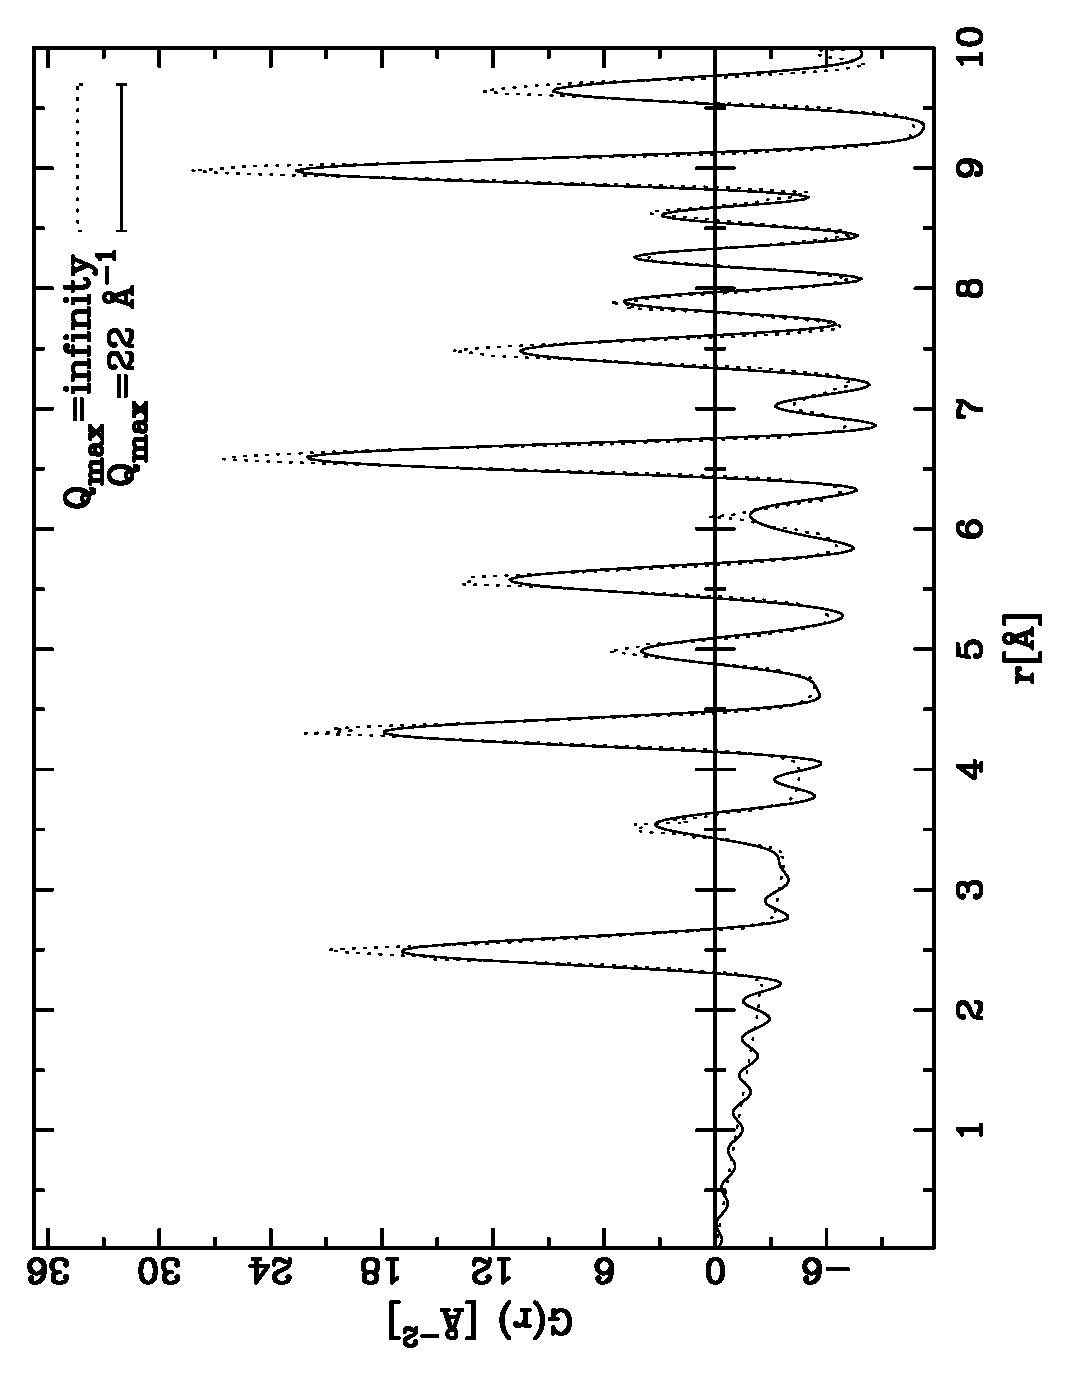
\includegraphics[scale=0.5, angle=270]{pdf.1.eps}
   \caption{Calculated PDFs of $Ni$}
   \label{pdf-fig1}
\end{figure}
%

\begin{MacVerbatim}
      1 read
      2 cell ni.cll,5,5,5
      3 #
      4 therm
      5 #
      6 pdf
      7   set rang,10.0,0.02
      8   set qmax,20.0
      9   set qdamp,0.0
     10   set rad,xray
     11 #
     12   calc
     13 #
     14   save pdf,ni.pdf
     15 exit
\end{MacVerbatim}
%
The macro file used to calculate the Nickel PDFs is listed above.
First we read the unit cell for Nickel and expand it to a size of
5x5x5 unit cells (lines 1--2). Next we introduce thermal vibrations
according to the given isotropic Debye-Waller factor (line 4). After
entering the PDF sub level (line 6) we specify the maximum value of
$r$ and grid size $\Delta r$ (line 7). In our case we calculate up
to a value of $r=10$\AA\ using a grid of $\Delta r=0.02$\AA. The
next command (line 8) specifies the value of $Q_{max}$ to be set to
20\AA$^{-1}$. Finally we set dampening term $\sigma_{Q}$ to 
zero (line 9) meaning
no Q-resolution correction and select X-ray radiation (line 10). Now
we are ready to calculate the PDF, done in line 12. All we have to
do now is to save the result to a file (line 14). The result is
shown in figure \ref{pdf-fig1}. \par

When discussing equation (\ref{eq_igr}) used to calculate the PDF
from a structural model, we just stated that the sum over $ij$ goes
over {\it all} pairs of atoms $i$ and $j$ within the model crystal.
This is perfectly correct to calculate a total PDF. However
sometimes it might be desired to calculate just a partial or
differential PDF. by selecting the elements of interest.

%------------------------------------------------------------------------

\section{Refining a PDF \label{pdf-rmc}}

In principle an experimental PDF can be refined based on a
structural model in two different ways. A relatively small model can
be refined using {\it PDFFIT}. On the other hand a larger model can
be refined using the Reverse Monte Carlo (RMC) algorithm in 
\discus. Details about the principle of RMC are discussed in chapter
\ref{rmc} of this manual. The only difference is that rather than
refining the scattering intensity directly, the PDF is refined. An
example refinement of a Nickel PDF is listed below and is also part
of the online tutorial of \discus.
%

\begin{MacVerbatim}
      1 read
      2 cell ni.stru
      3 #
      4 pdf
      5   data ni.data
      6 #
      7   set frange,1.5,10.0
      8   set qmax,22.0
      9   set rad,xray
     10   sel ni
     11   set mode,shift
     12   set move,ni,0.01,0.01,0.01
     13   set disp,1
     14   set cyc,25
     15   show all
     16   run
     17   save pdf,rmc.pdf
     18   save stru,rmc.stru
     19 exit
\end{MacVerbatim}
%
In lines 1--2 the starting structure is read. Next the {\tt pdf}
sub level is entered (line 4). First we read the observed PDF from
the file {\it ni.data}. The maximum $r$ and $\Delta r$ which defines
the range of the calculated PDF are taken from the data file just
read. Then the range in $r$ that actually should be used for the
refinement is set (line 7), here from 1.5 to 10.0\AA. In lines 8--9
the value of $Q_{max}$ and the radiation used in the experiment is
set. Now we enter the RMC related settings (see also \ref{rmc}). We
select atoms to be moved (line 10), here Ni. This command should not
be confused with {\tt isel} or {\tt jsel} which actually selects the
atoms that are included in the calculation of the PDF. The RMC mode
is set to shift atoms using a Gaussian distribution with a sigma of
0.01 lattice units ($\approx 0.035$\AA) in lines 11--12. Finally we
set the screen update interval to 1 (line 13) and specify that 25
cycles will be carried out (line 14). Before the refinement is
started in line 16, the current settings are displayed using the
command {\tt show} (line 15). After the refinement is finished, the
resulting PDF (line 17) and structure (line 18) is saved to a file.
\par

%------------------------------------------------------------------------

%------------------------------------------------------------------------
% Chapter:  RMC simulation
%------------------------------------------------------------------------

\chapter{Reverse Monte Carlo \label{rmc}}

This chapter gives a short introduction into the RMC level of 
\discus. \Discus can be used to either refine the scattering
intensities directly of to refine the atomic pair distribution
function (PDF) (see chapter \ref{pdf}). A more detailed description of the
various commands can be found in the reference manual or the online
help function.

%------------------------------------------------------------------------

\section{Introduction \label{rmc-int}}

The {\bf R}everse {\bf M}onte {\bf C}arlo (RMC) method
\citep{mcpu88} is another application of the Monte Carlo algorithm
discussed in chapter \ref{mc}.  Here, rather than minimizing the
total energy of the crystal, the difference between observed and
calculated intensity is minimized. Although the method has been
around for about 10 years, the method was first applied to {\it
single crystal} diffuse scattering in a neutron diffraction study on
ice {\it Ih} \citep{nikemc95}. \par

The RMC process starts also with the selection of a random site
and changing its variables like occupancy or displacement by a
random amount. The scattering intensity is recalculated for the
generated move and the goodness-of-fit parameter $\chi^{2}$ as
given in equation \ref{eq-chi2-1} is computed.
%
\begin{equation}
    \chi^{2} = \sum_{i=1}^{N} \frac { [ I_{e}({\bf h}_{i}) -
               I_{c}({\bf h}_{i}) ] ^{2}} { \sigma^{2} }
    \label{eq-chi2-1}
\end{equation}
%
The sum is over all measured data points ${\bf h}_{i}$, $I_{e}$
stands for the experimental and $I_{c}$ for the calculated
intensity.  The change in the goodness-of-fit is given by $\Delta
\chi^{2} = \chi_{old}^{2} - \chi_{new}^{2}$.  Every move which
improves the fit to the data ($\Delta \chi^{2} < 0$) is accepted.
Those moves which worsen the fit ($\Delta \chi^{2} > 0$) are
accepted with a probability of $P = exp(-\Delta \chi^{2} / 2)$. The
parameter $\sigma$ is assumed to be independent of {\bf h} and is
treated as a parameter of the modeling.  The value $\sigma$ can be
identified with the temperature T in the (direct) Monte Carlo method
described in chapter \ref{mc}.  How many {\it bad} moves are
accepted depends on the value of $\sigma$ or T.  \par

%------------------------------------------------------------------------

\section{RMC in more detail \label{rmc-detail}}

For practical use it is necessary to include a scaling factor $f$
and a background parameter $b$ in the definition of the
goodness-of-fit $\chi^{2}$. A weight $w({\bf h})$ is included as
well. \Discus allows the user to choose a particular weighting
scheme or to read weights from a separate input file. The definition
of $\chi^{2}$ used in the program is given in equation
\ref{eq-chi2-2}.
%
\begin{equation}
    \chi^{2} = \sum_{i=1}^{N} \frac { w({\bf h}_{i}) [ I_{e}({\bf h}_{i}) -
               (f \cdot I_{c}({\bf h}_{i}) + b) ] ^{2}} { \sigma^{2} }
    \label{eq-chi2-2}
\end{equation}
%
As in the previous section $I_{e}({\bf h}_{i})$ stands for the
measured intensity at the reciprocal point ${\bf h}_{i}$, and
$I_{c}({\bf h}_{i})$ is the calculated intensity in that point. The
summation is over all N experimental data points.  The value
$\sigma$ is a parameter of the modeling and controls the fraction of
{\it bad} moves which are accepted. The corresponding parameter in
(direct) Monte Carlo simulations is the temperature T.\par

Three different ways to calculate the scale $f$ and background $b$
are implemented. First the user can define fixed values for both:
$f = f_{0}, b = b_{0}$. Secondly, the background can be set to a
fixed value $b = b_{0}$ and the scaling factor $f$ is computed
according to equation \ref{eq-fb0}.
%
\begin{equation}
    f = \frac {\sum\limits_{i=1}^{N} w({\bf h}_{i}) I_{e}({\bf h}_{i})
                                             I_{c}({\bf h}_{i})
       - b_{0} \sum\limits_{i=1}^{N} w({\bf h}_{i}) I_{c}({\bf h}_{i})}
              {\sum\limits_{i=1}^{N} w({\bf h}_{i}) I_{c}^{2}({\bf h}_{i}) }
    \label{eq-fb0}
\end{equation}
%
Alternatively both values $f$ and $b$ can be refined during the
RMC refinement. Equation \ref{eq-fb} shows the corresponding
definitions.
%
\begin{eqnarray}
    f & = & \frac{\sum\limits_{i=1}^{N} w({\bf h}_{i})
                  \sum\limits_{i=1}^{N} w({\bf h}_{i})
                                        I_{e}({\bf h}_{i})I_{c}({\bf h}_{i})
                - \sum\limits_{i=1}^{N} w({\bf h}_{i}) I_{e}({\bf h}_{i})
                  \sum\limits_{i=1}^{N} w({\bf h}_{i}) I_{c}({\bf h}_{i})}
               {  \sum\limits_{i=1}^{N} w({\bf h}_{i})
                  \sum\limits_{i=1}^{N} w({\bf h}_{i}) I_{c}^{2}({\bf h}_{i})
         - \left (\sum\limits_{i=1}^{N} w({\bf h}_{i})
                                        I_{c}({\bf h}_{i}) \right ) ^{2} }
    \nonumber  \\
    b & = & \frac{\sum\limits_{i=1}^{N} w({\bf h}_{i}) I_{e}({\bf h}_{i})
        - f \cdot \sum\limits_{i=1}^{N} w({\bf h}_{i}) I_{c}({\bf h}_{i})}
                 {\sum\limits_{i=1}^{N} w({\bf h}_{i})}
    \label{eq-fb}
\end{eqnarray}
%
The scaling factor which the program prints on the screen during the
RMC refinement is actually (for some yet unknown reason) $1/f$.  The
parameters f and b are computed during each RMC cycle and usually
have large starting values as long as there are big differences
between calculated and observed data.  After every RMC move the
resulting scattering intensity and the $\chi^{2}$ value is
calculated.  In order to save computing time only the contribution
of the modified atoms to the scattering is calculated.  The
difference $\Delta \chi^{2} = \chi_{old}^{2} - \chi_{new}^{2}$ is
taken to decide if the move will be accepted or not.  If $\Delta
\chi^{2} < 0$ the agreement between calculated and measured data has
improved and the move is accepted.  Moves which result in a $\Delta
\chi^{2} > 0$ are only accepted with a probability of $P =
exp(-\Delta \chi^{2} / 2)$.  As the value of $\Delta \chi^{2}$ is
proportional to $1 / \sigma^{2}$, the value of $\sigma$ has an
influence on the amount of {\it bad} moves which will be accepted.
Obviously there are two extremes: For very large values of $\sigma$,
the experimental data are ignored ($\chi^{2} \approx 0$) and with
very small values of $\sigma$ the fit ends up in the local minimum
closest to the starting point, because there is a negligible
probability for {\it bad} moves.  In order to be more independent of
the actual number of data points used, the goodness-of-fit parameter
used in the program is given by $\chi^{2} / \sum w({\bf h}_{i})$.
The program calculates separate scaling factors and background
parameters for every used plane of experimental data.  This allows
to simultaneously use data measured with X-rays and neutrons,
different wavelengths or from different instruments.  The
goodness-of-fit $\chi^{2}$ is displayed as its total value and
separate for each data plane.

%------------------------------------------------------------------------

\section{Setting up a model crystal \label{rmc-cryst}}

The first step in an RMC refinement is the creation of a model
crystal of suitable size.  In many cases the starting structure will
be the (known) average structure for the compound under
investigation.  Since certain information of the crystal (e.g.
symmetry) is used in the RMC segment, it is advisable to {\bf to set
the crystal before entering the RMC segment}. Depending on the kind
of disorder to be modeled it might be necessary to introduce
displacements according to the temperature factors (command 'therm',
see section \ref{mod-therm}) or create the needed amount of
vacancies before starting the RMC refinement.  How to generate a
crystal is described in chapter \ref{struc}, tools to modify the
crystal are discussed in chapters \ref{mod-simple} and
\ref{mod}.\par

%------------------------------------------------------------------------

\section{Operation modes \label{rmc-mode}}

So far changes to the crystal made during the RMC refinement were
simply called 'moves'. These moves can either be a displacement of
an atom or the change of the occupancy of an atom site.  Because the
relative abundance of the elements is not allowed to change during
the simulation, the later move is actually made by switching the
atoms of two sites within the crystal. The program knows three
different operation modes which involve three different kinds of
moves shown in figure \ref{rmc-fig1}. Additionally user defined
moves can be included in an external subroutine linked to the
program \discus.
%
\begin{figure}[!tbh]
   \centering
   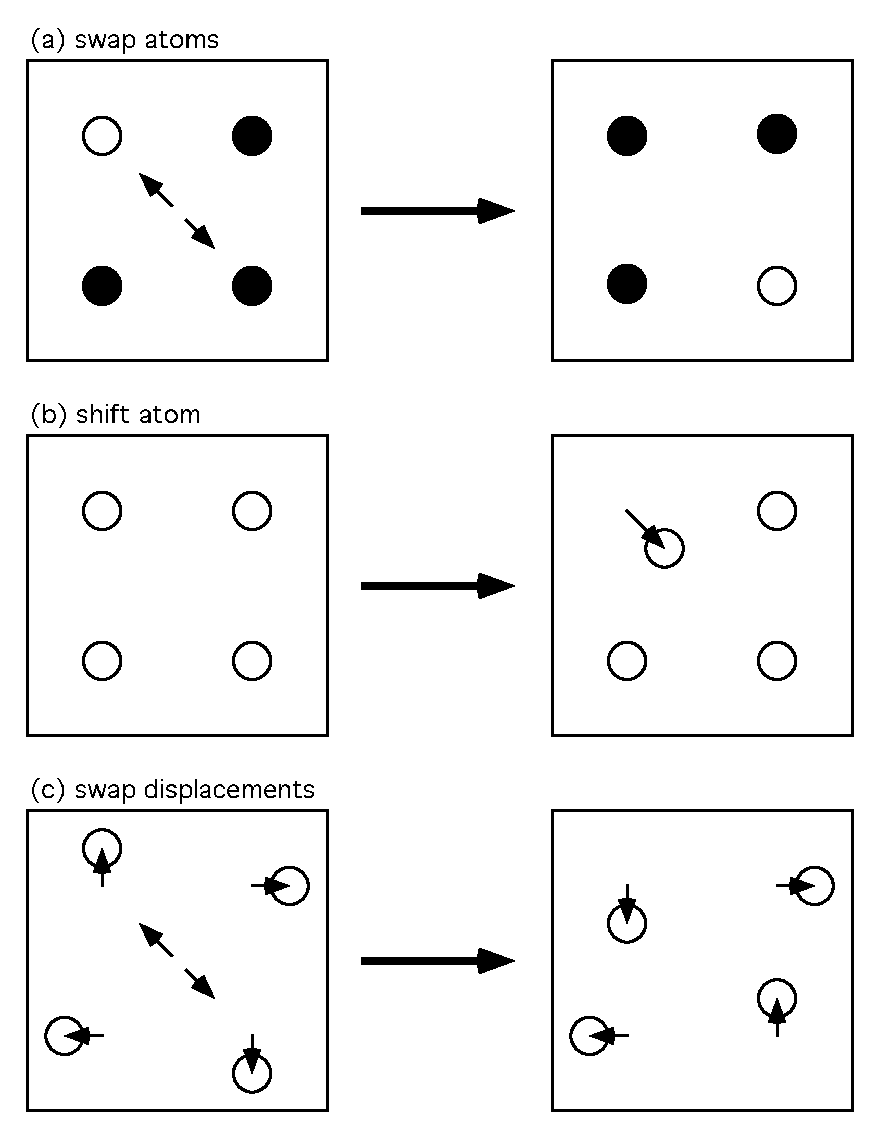
\includegraphics[scale=0.5, angle=0]{rmc.1.eps}
   \caption{RMC operation modes of \Discus }
   \label{rmc-fig1}
\end{figure}
%
A short description of the different RMC operation modes is given in
the list below.
%
\begin{enumerate}
    \item {\it switch chemistry}:
    This mode (Fig. \ref{rmc-fig1}a) allows to simulate occupational disorder
    by selecting two different atoms randomly and switch these two atoms. This
    operation mode can obviously work only, if at least two different types of
    atoms are present within the crystal.  This mode is selected by the
    command {\tt set mode, swchem}.

    \item {\it shift atom}:
    If this mode (Fig.  \ref{rmc-fig1}b) is set, a randomly selected atom is
    shifted by a random amount in a random direction.  The size of the
    generated shift is chosen uniformly in the interval [-1,1] unit cell.
    The actual shift applied to the atom is the generated shift multiplied
    with a user defined factor ('set move,$<$x$>$,$<$y$>$,$<$z$>$').
    These factors are also given in unit cell units.  The shift mode is
    selected by with {\tt set mode, shift}.

    \item {\it switch displacements}:
    This mode (Fig. \ref{rmc-fig1}c) is selected by the command {\tt set
    mode, swdisp} by swapping the displacement, i.e.  the difference between
    the average and the actual position, of two randomly selected atoms of
    the same type and thus the overall average displacements remain constant
    in contrast the previous mode.  The user has to make sure that initial
    displacements are present in the starting structure (e.g.  thermal
    displacements e.g.  by using the command {\tt therm}.

    \item {\it external}:
    The program \Discus allows the user to define more complex RMC
    moves via an external subroutine.  This subroutine is defined in the file
    {\it extrmc.f90}. For more details about the construction of such a
    subroutine, read the commented example in the file {\it extrmc.f90}
    which is part of the distribution.
\end{enumerate}
%
The program allows to select ({\tt sele $<$typ1$>$, $<$typ2$>$, ..})
and deselect ({\tt dsel $<$typ1$>$, $<$typ2$>$, ..}) atom types
which should be taken into account during the RMC simulation.
Alternatively molecules (if present) can be selected using the
commands {\tt msel $<$typ1$>$, $<$typ2$>$,..} and {\tt mdes
$<$typ1$>$, $<$typ2$>$, ..}. Here $<$typ$>$ is the corresponding
molecule type. All modes listed above can be used for these rigid
molecules as well.  Rotations and other symmetry operations can be
realized by creating the wanted different orientations of the
molecules as different types using the symmetry segment of 
\Discus (see chapter \ref{cryst-sym}) and subsequently using the
'swap chemistry' mode. After every generated move the minimal
allowed distances ({\tt set mdis, $<$atom1$>$, $<$atom1$>$,
$<$dist$>$}) between all selected atoms are checked and if atoms are
too close, the move is rejected.

%------------------------------------------------------------------------

\section{Running RMC \label{rmc-run}}

Finally, the experimental data need to be read before the RMC
refinement can start.  The file format for the experimental input
data is similar to the output formats \Kuplot and {\it PGM} for
the Fourier transform.  It might be necessary to remove Bragg peaks
and other unwanted scattering (e.g.  powder rings from a sample
holder) from the input data set. With the {\tt data} command, the
method (neutron or X-ray), weighting scheme and the corners of the
input data set in reciprocal space are entered.  More than one plane
of experimental data can be read by repeating the 'data' command.
After the data have been read, select the desired RMC mode, select
the appropriate atoms and start the refinement with the {\tt run}
command.
%

\begin{MacVerbatim}
   Gen:   1200 try:    352 acc: (good/bad):     62 /      0 s2x2:   11829643.
     Plane  1: scal:  14.83     / back:  22.23     / s2x2:          11829643.
\end{MacVerbatim}
%
The screen output is updated in a user defined interval, an example
output is shown above.  The fist line gives the number of generated
moves ('Gen') and how many of those were actually tested ('try').
The difference is due to selecting atoms that should not take part
in the refinement and moves that violate minimal atom distances. The
next two numbers give the number of good ($\Delta \chi^{2} < 0$) and
bad ($\Delta \chi^{2} > 0$) moves that have been accepted.  The last
number is the current value of the overall $\chi^{2}$ for all data
planes.  Additionally the scaling factor $f$ and the background $b$
are given for each data plane (one in this example) followed by
$\chi^{2}$ for the corresponding data plane.  The resulting
structure as well as the calculated scattering can be saved with the
{\tt save} command.

%------------------------------------------------------------------------

%------------------------------------------------------------------------
% Chapter:  Experimental data conversion 
%------------------------------------------------------------------------

\chapter{Experimental data treatment \label{data}}

This chapter illustrates the capabilities of \Discus to treat experimental
data for further analysis.

\section{Powder PDF \label{data-pdf}}

The atomic pair distribution function (PDF) can be obtained from
powder diffraction data and is a valuable tools for the study of the
{\it local} atomic arrangements in a material. This section 
describes how \Discus can be used to transform an experimental powder
diffraction pattern to a powder PDF.

The commonly used powder PDF is obtained from the reduced normalized 
intensity via a sine Fourier transform.

\begin{equation}
  G_{obs}(r) = \frac{2}{\pi} \int_{Q_{min}}^{Q_{max}}  F(Q) sin(Qr) dr
  \label{eq_f2gr}
\end{equation}

where F(Q) is obtained from the normalized intensity as:
 
\begin{equation}
  F(Q)       = Q [ S(Q) - 1 ] 
\end{equation}

The normalized intensity in turn is generated from the experimental
powder diffraction pattern through the application of several corrections. 
These corrections treat aspects like treat inelastic scattering etc.

For quite some time now, empirical corrections are used that turn out to
perform a good job, see \cite{bifa2013} for more detaiuled discussion. 
The algorithm in \Discus essentially performs along the lines described 
in \cite{bifa2013}.

\subsection{Treatment of powder data in \Discus \label{data-pdf-treat}}

The experimental powder pattern is transformed within \Discus by performing
the following steps:

First the input data are transformed onto an equidistant grid in Q-space.
The same is done for background data, if the user provided a background 
measurement. The initial steps along Q for the powder pattern and the 
background pattern do not have to be identical. The only two requirements 
are that
Q$_{min}$ of the powder data is equal or lower than the corresponding 
limit for the powder data. And secondly that the background Q$_{max}$
is higher that the limit for the data.

If background data are provided, these are subtracted from the powder
intensities. An optional scale factor allows to take different counting 
times into account.

\begin{equation}
  I_p (Q) = I_{obs} * scale \cdot Background
\end{equation}

Next \Discus calculates the average form factors squared 
$\langle f \rangle^2$, using 
the composition provided by the user or alternatively the composition of the
current structure. This step is essential, as it is the only multiplicative
correction that is applied. The user should ensure that the composition is
correct or at least close to the actual composition.

\begin{equation}
  I_i (Q) = \frac {I_{p}} {\langle f \rangle^2}  
\end{equation}

The result is point wise multiplied by Q to obtain an intermediate step 
towards F(Q). 

\begin{equation}
  F_i (Q) = Q \cdot  I_{i}(Q) 
\end{equation}

The next step is the empirical transformation into the actual F(Q). A 
polynomial function is fitted through these intermediate
data. The order of the polynomial can be adapted by the user. The 
difference between the intermediate data and the polynomial is taken as
F(Q). As the order of the polynomial should be kep moderately low, the 
polynomial itself is a slowly varying function in reciprocal space. Its 
highest frequency is much lower than that of the actual diffraction signal by 
the sample.

\begin{equation}
  F(Q) = F_i (Q) - \sum_i p_i  \cdot Q^i
\end{equation}

At this point the Q-scale can be adapted, which is likely necessary for 
electron diffraction data only. As the effective camera length might vary
slightly, \Discus allowes to determine the peak position of a significant 
maximmum in F(Q) and to scale the Q-axis with a multiplicative operation 
to set the peak position to a user provided expected value. Be aware that
this scaleing operation effectively prohibits any interpretation of 
absolute interatomic distances. Relative lengths of different pair distances
also affected by this scale.

The empirical transformation of the powder intensity onto F(Q) does not
include a transformation onto an absolute scale. Instead \Discus applies a
multiplicative operation to F(Q) to put this onto an empirically determined 
approximate absolute scale. This the integral over a peak in G(r) does not
allow you to determine an absolute coordination number. As the powder 
diffraction menu in \Discus includes a multiplicative scale factor you can
still fit the parameters of a model structure to obtain a match between 
the observed and experimental PDF.

As last step \Discus applies Eq. \ref{eq_f2gr} to obtain the observed
powder PDF. User supplied limits allow to flexibly write different 
sections of the PDF.

\subsection{Example \label{data-pdf-exa1}}

The macro in this example illustrates such a data transformation in \discus.

\begin{MacVerbatim}
 1 exp2pdf
 2 reset
 3 data xy, DATA/powder.inte
 4 back xy, DATA/background.inte, scale:1.0
 5 radiation xray
 6 comp comp:ZnO
 7 limits inst:30.0, fourier:29.5, qmin:0.90
 8 poly order:9
 9 qscale qobs:2.00, qcrystal:2.001
10 output gr:GROBS/sample.grobs, rmin:0.01, rmax:100.00, rstep:0.01
11 output iq:GROBS/sample.iqobs
12 output sq:GROBS/sample.sqobs
13 output fq:GROBS/sample.fqobs
14 run mode:inter
15 exit  ! Back to the main DISCUS menu
\end{MacVerbatim}

The \Discus command {\tt exp2pdf} steps into the data treatment menu.
As for all menus in \Discus the {\tt reset} command (line 2) allows you to ensure that all 
parameters are reset to their initial values at program start.

In lines 3 and 4 the experimental data and the background are read from the 
corresponding input files. \Discus can handle several input formats like
simples 2 or 4 column ASCII files, Spec type files or generic CSV type files.
See the on-line help in \Kuplot for the {\tt load} command for further details.

The empirical algorithm in \Discus can be applied to {\tt xray}, {\tt neutron}
or {\tt electron} diffraction data, simply choose the appropriate value on the 
{\tt radiation} command (line 5).

The composition is set in line 6 with {\tt comp} command. You can specify the 
actiul composition either with the optional parameter {\tt comp:} followed 
by a chemical statement or likewise just as a simple parameter on the 
{\tt comp} command line. The composition should be specified as a list of
atom names, optionally followed by the (relative) abundance. At names must have
a capital first letter and a lower case second letter. Spaces are irrelevant. 
Internally \Discus normalizes the sum of all element abundances to 1.
Thus the following lines would give exactly the same composition:  

\begin{MacVerbatim}
comp comp:Zno
comp comp:Zn1.0O1.0
comp comp:Zn 1.0 O 1.0
comp Zn 2 O 2.0
\end{MacVerbatim}

Alternatively you can use the current structure with in \Discus to specify the 
composition, in this case the command should be:

\begin{MacVerbatim}
comp comp:current
\end{MacVerbatim}

As data at high Q values might be affected by high noise level and detector 
artefacts, \Discus allows yo to limit the upper Q-value to an {\tt instrumental}
value on the {\tt limits} command line. Data above this Q-value will  be 
ignored and have no effect on the calculations. 

To avoid unnecessary Fourier termination ripples, the sine-Fourier transform
of Eq. \ref{eq_f2gr} should be limited at a Q$_{max}$ where F(Q$_{max}$) is zero. 
\Discus will teremine such a Q$_{max}$ value either below Q$_{max;inst}$ or
close to a user supplied value on the {\tt fourier:} parameter.

The lower limit Q$_{min}$ in the integeral, Eq. \ref{eq_f2gr} usually is less
critical. Most of the times \Discus can determine this value automatically 
as the first significant minimum in F(Q). Data below Q$_{min}$ are replaced
by a straight line to the point Q=0; F(0) = 0.

The default polynomial extends to 7the order. An indication that this order 
is too low is a peak in the experimental G(r) at very short distance below 0.5\AA{}.
If necessary try to expand the order. As a further test, run the following macro
within \Kuplot immediately after the {\tt exp2pdf} macro is finished.
 
\begin{MacVerbatim}
fit n[1]
show
exit
\end{MacVerbatim}

As the transformation creates as last \Kuplot data set F(Q). The macro will
list the parameter values and their estimated uncertainty. Ensure that the 
highest order are still significant.

The observed PDF is always written into a default file name. Most of the
times though the user will choose a suitable file name and suitable 
limits for the distance r on a {\tt output} command line, line 10. In the 
example output data will be witten into the directory {\tt GROBS}, 
file {\tt sample.grobs}. The distance values on teh optional parameters
{\tt rmin}, {\tt rmax} and {\tt rstep} are understood as \AA{}.

If the output file name starts with the string "kuplot", the output is not
written to disk but placed into KUPLOT as last dat set.

No further output is written, unless the user explicitely states the
optional parameters {\tt iq:}, {\tt sq:} and / or {\tt fq:} with an 
appropriate output file name. These optional parameter cann all be stated on the 
same {\tt output} command line or on individual lines as in the example.

Finally the operation is performed with the {\tt run} command on line 14.
As optional parameter {\tt mode} you can specify "inter" or "silent", the 
latter being the default if the {\tt mode:} parameter is omitted. With 
{\tt mode:silent} \Discus produces no further output until the menu is finished. 

In interactive mode, intermediate data are displayed. In interactive mode,
if the optional parameter {\tt fourier:} has been omitted, \Discus allows you to 
choose this value during the calculation.

Fig \ref{data-pdf-fig1} shows the experimental intensity and background that
is displayed in interactive mode. Note that the background has not yet been scaled.
%
\begin{figure}[!b]
   \centering
   \includegraphics[scale=0.4, angle=270]{iq_initial.eps}
   \vspace*{+5mm} 
   \caption{Initial intensity and background}
   \label{data-pdf-fig1}
\end{figure}
%
Fig \ref{data-pdf-fig2} shows the final F(Q). The vertical red line mark the
lower and upper limits. The upper limit Q$_{max;fourier}$ has already been 
adjusted to a position at which F(Q$_{max;fourier}$) is zero.

The vertical green line marks the peak position used for the adjustment of the
Q-scale. As \Discus will search for the highest peak with a wide window of 
0.25\AA$^{-1}$ width, choose the highest maximum in the lower Q-range. 
%
\begin{figure}[!b]
   \centering
   \includegraphics[scale=0.4, angle=270]{fq_final.eps}
   \vspace*{+5mm} 
   \caption{Final F(Q). The lower frame shows the last 4\AA$^{-1}$ to
            choose Q$_{max;fourier}$, The vertical green line shows
            the peak postion used for the optional adjustment of the Q-scale.}
   \label{data-pdf-fig2}
\end{figure}
%

Finally Fig \ref{data-pdf-fig3} shows the final G(r). 

%
\begin{figure}[!b]
   \centering
   \includegraphics[scale=0.4, angle=270]{gr_final.eps}
   \vspace*{+5mm} 
   \caption{Final G(r). Note the absence of any Fourier ripples and the
            absence of any spurious peak in the low distance range.}
   \label{data-pdf-fig3}
\end{figure}
%

%\par

%------------------------------------------------------------------------


%------------------------------------------------------------------------
% Appendices
%------------------------------------------------------------------------

\appendix
\chapter{DISCUS commands}
\section{Summary}
\par
\begin{MacVerbatim}
News       ! Summary of recent changes
addf       ! Add two files together
append     ! Append atom to model crystal
asym       ! Show the contents of the asymmetric unit
boundary   ! Cuts off atoms along an hkl plane
branch     ! Switches to KUPLOT, if within the suite
change     ! Changes the character of an object
chem       ! Enter CHEM level (see chem level for details)
connect    ! Enter CONNECTIVITY level
copy       ! Copy atom or molecule within the crystal
export     ! Exports the structure in a different format
decorate   ! Enter  DECORATE level
d2r        ! Transform vector from real to reciprocal space
define     ! Define DISCUS specific settings
diff-four  ! Enter DIFFERENCE FOURIER transform level
domain     ! Enter the DOMAIN level
find       ! Find atoms around a given point
four       ! Enter FOURIER transform level
import     ! Imports other formats into DISCUS cells
ins        ! Insert atom or molecule into the crystal
inverse    ! Enter inverse Fourier transform level
kick       ! Insert atom/molecule and possibly remove old atom/mole.
mmc        ! Enter MONTE-CARLO simulations level
output     ! Enter output level (save results)
patterson  ! Enter PATTERSON level
pdf        ! Enter PAIR DISTRIBUTION FUNCTION level
plot       ! Enter PLOT level (export crystal for plotting)
powder     ! Enter POWDER diffraction level
project    ! Calculate projections in real and reciprocal space
property   ! Enter the PROPERTY level
purge      ! Remove voids from crystal (DO NOT USE !)
r2d        ! Transform vector from reciprocal to real space
read       ! Read structure or unit cell from file
remove     ! Remove atom or molecule from crystal
replace    ! Replace atom(s) or molecule(s) with other type
reset      ! Reset DISCUS to initial program start conditions
rmc        ! Enter REVERSE-MONTE-CARLO level
save       ! Enter SAVE level to save the structure
seed       ! Set seed for random number generator
shear      ! Enter the SHEAR level
show       ! Show various information
spacegroup ! Sets the space group for the current structure
stack      ! Enter STACKING FAULT level
storage    ! Enter STORAGE level
switch     ! Swap two atoms or molecules within crystal
symm       ! Enter SYMMETRY transformation level
transform  ! Enter unit cell TRANSFORMATION  level
therm      ! Displace atoms or molecules according to B
vprod      ! Calculate vector product in real or reciprocal space
waves      ! Enter WAVE type modulations level
wyckoff    ! Shows symmetry operations of the space group
\end{MacVerbatim}
\section{News}
\par
Here you find a list of recent changes, additions, bug corrections 
\subsection*{2019\_Dec}
\par
mmc 
   The displacement correlation did not really work, fixed. 
\par
CIF interpreter 
   Further improvements to interpret CIF files. For unknown 
   space groups DISCUS attempts to use the symmetry operations. 
\subsection*{2018\_Nov}
\par
m[$ <$number$> $] 
   If an atom is removed, its scattering curve is set to zero and 
   the property 'normal' was cleared. 
   If you manually change the scattering curve back to a non-zero 
   value, the properies were not set back to 'normal' Fixed. 
\par
save 
   enforced that "scat", "adp" and "occ" and either all written 
   or all omitted. 
\par
powder 
   For neutron diffraction, the output of the $ <$f$> $$**$2 contained an 
   error. The negative scattering length were added as $| $b$| $. 
   Corrected. 
\par
mmc 
   Added a 'set valid, $ <$invalid\_moves$> $' command, that gives you more 
   control over a termination criterion. 
\par
CIF interpreter 
   Added more flexibility to recognize non standard monoclinic space 
   groups that are not listed as full Hermann-Mauguin symbol 
\subsection*{2018\_Oct}
\par
In ==$> $ 2017\_July the following "correction" was done, which proved 
to be false. 
The ==$> $ 'therm' command erroneously used too large a displacement. 
The average $ <$u$**$2$> $ were actually 3 times too large. 
\par
As of version 5.27.2 this has been corrected yet again to the 
original, correct state. A calculation of a powder /single crystal 
pattern either with "temp use" or a combination "therm and temp ignore" 
will now produce icdentical results again. 
\par
Added a 'show res' to the 'fourier' and 'connectivity' menu. 
\par
Improved the memory handling in pdf, makes the program use much 
less memory. 
Connected to this, all menus reduce memory usage through the 
local 'reset' command. The 'reset' command sets all default 
values within a menu back to program start and initializes all 
internal arrays to the smallest default size. Most of the time 
this will not bee needed. The main effect will be within the 
Fourier menues (fourier, powder, output). The 'pdf' menu is 
reduced as much as possible automatically. 
\par
\subsection*{2018\_Sep}
\par
Added new export options: 
to CIF 
export cif, $ <$filename$> $ 
\par
to RMCprofile version 6 and 7 
export rmcprofile, $ <$filename$> $ [,version:7] 
\par
to VASP, POSCAR file 
export vasp, POSCAR 
export poscar, POSCAR 
\par
If atom types exist, for which there is no more actual atom in 
the crystal, the form factors are set to zero. This alloes you 
to define pseudo atoms for the domain without the need to 
use the 'fourier/scat' command to set dummy scattering 
functions. 
\par
purge, stack, domain, deco 
   Turned on stricter behavior for the handling of 
   periodic boundary conditions and the "chem" quick mode 
   off. It can be turned back on with after explicit 
   'set crystal' comand in the chemistry menu. 
\par
added a 'reset to the 'chem' menu 
added a 'reset to the 'domain' menu 
added a 'reset to the 'fourier', 'inverse', difffour', patterson' menu 
added a 'reset to the 'insert' menu 
added a 'reset to the 'pdf' menu 
added a 'reset to the 'shear' menu 
added a 'reset to the 'save' menu 
added a 'reset to the 'stack' menu 
added a 'reset to the 'symmmetry' menu 
added a 'reset to the 'transform' menu 
added a 'reset to the 'waves' menu 
added to the global 'reset: 
    most arrays, chem, deco, domain, fourier routines, insert, mmc, 
    pdf, property, rmc, save, shear, symmetry, transform, waves 
\par
\subsection*{2018\_Aug}
\par
Added a 'reset' command to DISCUS. (Work in progress) 
Added a ==$> $ 'storage' menu. 
   This menu allos to display and manage the internally stored 
   crystal structure files. 
\subsection*{2018\_July}
\par
Added the possibility to define property like features 
that are based on the connectivities ==$> $ property 
\par
Fixed a bug that did not allow a read free for origin choice 2 
Added an 'exit' command to the read menu. 
\par
Added a 'reset' command to 'plot' 
\par
connectivity 
   Modified the behavior for central atoms given by name 
   instead of type number. Connectivity will perform the 
   requested action for all atom types of this name. 
   add Si, O, 1.2, 2.0, silicon 
   Creates a connectivity for all Silicon atom types. 
\par
\subsection*{2018\_June}
\par
Added the possibility for interactive plots. 
See ==$> $ plot/back 
    ==$> $ plot/poly 
    ==$> $ plot/bond 
    ==$> $ plot/run 
\par
Revised the reaction to a CTRL-C 
\par
Added a ==$> $ 'set error, ... , "save" option 
\par
functions 
\par
Added a new logical function that querries the properties of an atom. 
\par
decoration 
Added a "chelate" bonding scheme and corrected the descriptions 
for the "bridge" scheme. 
Added the missing descriptions to the "acceptor" and "donor" 
schemes. 
\subsection*{2018\_May}
\par
surface 
Corrected a BUG related to the location of cylindrical surfaces. 
\par
read / import 
Improved handling of CIF files with atom names like "Ti4+" 
Improved handling of CIF files with atom lines that contain 
just dots 
Ti Ti 0.00 0.00 0.00 . 1.0 
\subsection*{2018\_April}
\par
remove molecules 
Changed the behavior if whole molecules are removed. The 
molecule type is still set to zero and the atoms inside the 
molecule are switched to 'voids'. The molecule status of the 
individual atoms is, however, retained. This allows you to still 
wotk with these "removed" molecules, in strict analogy to 
removed atoms. The full molecule entry disappears with a 'purge' 
\par
occupancy 
An 'occupancy' was added as further atom property. 
The philosophy behind DISCUS is a simulation of an actual 
crystal structure, thus the occupancy is really just an 
emergency measure for the simulation where you want just 
very few or a single unit cell. 
As side effect the format of the 'cell' file has been 
augmented. 
For details see ==$> $ 'read' 
\par
read / import 
Improved handling of CIF files that do not have an empty 
line following a 'loop'. 
Import the occupancy. 
\subsection*{2018\_Mar}
\par
save 
As of version 5.17.1 DISCUS saves the atoms in its internal 
sequence, even if molecules are involved. The molecule info 
is written into the file header and further columns have been 
added to the atom list that specify in which molecule an atom 
is located. 
\par
stack 
A simplified list of origin types has been added to the 
'create' command. This list "internal.stacksimple.list" 
contains the atom types "L001", etc at reduced origins 
starting at 0,0,0 and incrementing with [0,0,1]. This 
list facilitates correlation analysis. 
\par
read 
A comment with the read menu caused an exit, changed to 
ignore the comment. 
\par
read / import 
Improved the reading of CIF files. Attempt to replace ion 
charges with the DISCUS standard as best as possible. 
If the space group is not given or is a '?', the symmetry 
operations are read instead. 
\subsection*{2018\_Jan}
\par
The logical comparisons may now take the operators: 
$ <$, $ <$=, ==, /=, $> $=, $> $/ 
The classical fortran77 operators are still valid 
\par
New logical functions "isvar" and "isexp" can be used within an 
"if" construction. See help entry ==$> $'function' in the 
general "Command\_lang" section. 
\par
Variable "mol\_type[$ <$i$> $]" has been made read/write 
\par
stack 
The ==$> $ 'create' command copies the list of layer origins 
into an internal file with fixed name "internal.stacklist.stru" 
\subsection*{2017\_Nov}
\par
Added RMCprofile version 6 format to imports 
\par
Added an "export" command, currently just a "shelx" export format 
\par
Added a choice to the ==$> $ 'symmetry/mode' command 
Added the possibility to use a space group symmetry matrix. 
Related is the new variable sym\_n[1] that stands for the 
number of symmetry operations in the present space group. 
\par
Added optional parameter 'identical:' to read /cell command 
\par
Added a command 'spacegroup' that sets the sace group. 
\par
The 'wyckoff' command returns the multiplicity of the site and 
the spacegroup symmetry matrices that copy the site onto itslef. 
\subsection*{2017\_Oct}
\par
Space Groups 
  Added the space groups 
  Aem2=Abm2 (39) 
  Aea2=Aba2 (41) 
  Cmca=Cmce (64) 
  Cmma=Cmme (67) 
  Ccca=Ccce (68) 
\par
Atom names 
  Instead of atom names or numbers, the user can specify a 
  user defined variable. 
  variable character, string 
  string = 'Si' 
  ... 
  sel  Al, string, O 
  ... 
  replace Al,string,... 
\par
connectivity 
  New optional parameters allows to specify if the connectivity is to 
  be restricted to the same molecule as the central atom. 
\par
stack 
  The number of layers for each type is recorded into 
  the result variable. 
\par
surface 
  The boundaries have improved and corrected behavior for internal 
  hollow spaces created by the "outside" flag. 
\par
  The boundary commands create a new variable that reflects the 
  surface character and the direction of the normal to the local 
  surface. 
\subsection*{2017\_Sep}
\par
Throughout the program the internal calculation of random numbers 
was changed to the FORTRAN 90 intrinsic function. 
\subsection*{2017\_July}
\par
The decoration of ligands onto surfaces can now be restricted to 
specific faces. 
\par
The ==$> $ 'therm' command erroneously used too large a displacement. 
The average $ <$u$**$2$> $ were actually 3 times too large. 
\subsection*{2017\_June}
\par
Atom "AL3+" had been misspelled internally. 
\par
The 'hkl' command in 'fourier' can now handle format strings for 
the file name. 
\subsection*{2017\_May}
\par
The boundary command at the top level menu and inside the surface 
menu can now create a polyhedron from a form of symmetrically 
equivalent hkl planes as well as a triaxial ellipsoid. 
The command at the main discus level is depreciated and you are 
encouraged to use the (identical) command at the surface menu. 
\subsection*{2017\_April}
\par
The surface menu received a new command "char" that determines 
the surface character of an atom. 
\subsection*{2017\_March}
\par
The 'read' ==$> $ 'cell' and 'stru' commands have been changed to 
accept CIF, CMAKER and RMCprofile formats as well. 
\par
The molecularize command will add atoms to a previous molecule, if 
the first atom is inside a molecule. 
\subsection*{2017\_Feb}
\par
Within the powder menu, the energy of the radiation may also 
be specified via ==$> $ 'set energy, $ <$value$> $' 
\subsection*{2017\_Jan}
\par
A new command 'first' was added to 'stack' that allows to determine 
the first layer type 
\par
An unfortunate typing error in News/2016\_Oct regarding the new 
refinement variable 
ref\_para[1...]   ( was misspelled as ref\_param[1...] ) 
is corrected in the  on-line help. 
\subsection*{2016\_Dec}
\par
At a few select points colors are introduced into the output. 
Currently these are just the error messages. 
\par
The new "molecularize" command allows to group atoms into molecules 
\subsection*{2016\_Oct}
\par
The output of the "blen" and "bang" commands within "chemistry" 
is now written to KUPLOT directly, if the filename starts with 
"kuplot" 
\par
The data stored by ==$> $ 'chemistry' ==$> $ 'aver' have been changed in 
a non-backwards compatible way. DISCUS now stores 9 values per 
atom: 
the site number, the atom type on this site, the position, 
the standard deviation of the average position and the occupancy. 
\par
If DISCUS detects more than one "data\_" sections in a CIF file, 
the second etc sections are written to a separate file, augmented by 
a number 
\par
Global variables have been introduced that use the same syntax as 
user defined variables. This include just "pi" and variables related 
to the refinement. 
DIFFEV sets the value to these variables: 
REF\_GENERATION  Current generation 
REF\_MEMBER      Current population size 
REF\_CHILDREN    Current children size 
REF\_DIMENSION   Number of parameters 
REF\_KID         Current child Updated for DISCUS and KUPLOT only 
REF\_INDIV       Current individuum Updated for DISCUS and KUPLOT only 
ref\_para[1..]   Current trial parameters for current child 
\par
Insertion of a new atom will automatically turn off the periodic 
boundary conditions. 
\par
Periodic boundary conditions in combination with the exact search mode 
have been enabled. 
\par
A new menu is introduced that allows to group atoms into a molecule. 
\par
The symmetry commands 'uvw' and 'orient' have been improved to allow 
to specify a pair, respectively one atom to define the axis/origin 
\par
The symmetry command can now rotate partial molecule groups 
\par
A new 'recreate' command allows to rebuild the connectivity list 
for a specific atom type while leaving the remainder intact. 
\subsection*{2016\_June}
\par
The mmc 'set move' command may now take a further parameter. This 
will actually restrict the movement of the specified atom along 
the direction of a vector. 
\par
DISCUS may now be interrupted gracefully with a CTRL-c. 
This will cause DISCUS to write the current structure 
as a file called EMERGENCY.STRU. 
\subsection*{2016\_May}
\par
Added option to the save menu to utilize the atom properties. 
\subsection*{2016\_March}
\par
Within the ==$> $ fourier menu, the radiation may also be defined 
via its ==$> $ 'energy' instead of its wavelength ==$> $ 'wvle' 
\par
Domains with an explicit shape (cube, sphere, cylinder) can now 
be generated with a size distribution. 
\par
Fourier can calculate the intensities for a SHELXL file 
\par
The 'find env' command will now return the neighbors sorted by distance. 
\par
2D and 2D images can be written in MRC file format 
\par
The ==$> $ 'add' command within the ==$> $ 'connectivity' menu can now take 
a new optional parameter that restricts the connectivity to the 
closest N atoms. 
\subsection*{2015\_Dec}
\par
Added a command 'apply\_symmetry' to the chemistry and mmc menus. 
These allow to generate symmetry equivalent correlation vectors. 
See mmc and chem ==$> $ set vec; set neig; apply\_symmetry for more help 
\par
Added the option to calculate normalized intensities for single 
crystal pattern. 
\subsection*{2015July\_A}
\par
You can now write powder files as normalized scattering function S(Q) 
or as reduced normalized scattering function F(Q) = Q[S(Q)-1] 
\par
\subsection*{2015July}
\par
With the release of the DISCUS\_SUITE several new capabilities have 
been introduced. 
\par
Within the DISCUS\_SUITE the output files can be written directly into 
KUPLOT. Simply start the file name with the fixed string 'kuplot'. 
The data set number in kuplot will be incremented automatically. 
\par
DISCUS contains the new ==$> $ 'branch' command that allows you to 
change to a KUPLOT or DIFFEV section. 
\subsection*{2015February}
\par
The speed of the PDF and powder(Debye) calculations has been improved 
considerably. No side effects on the user. 
\par
DISCUS does check if an atom in the unit cell file has a name "void" 
and it will ignore these atom types when calculating the PDF. 
This helps to get the proper PDF density and weights for molecules 
where the first atom is a void at the center of the molecule. 
\subsection*{2014November}
\par
DISCUS will now import CIF files, see ==$> $ import 
\par
\subsection*{2013September}
\par
The chemical short range order in mmc can now sort groups of 
atom types. 
\par
\subsection*{2013June}
\par
Finally this is it! DISCUS is now a fortran2008 program. Most of the 
substantial changes should not affect the user (or so we hope). 
Most of the large arrays are now allocated automatically, as needed, 
thus the need to compile DISCUS with different size versions should 
no longer exist. 
\par
\subsubsection{Command\_line\_options}
\par
The command line may now take the additional option: 
program -macro $ <$macro\_name$> $ [$ <$par1$> $ [ $ <$par2$> $ ...]] 
\subsubsection{Electron}
\par
DISCUS now offers electron diffraction in the kinematical limit as well. 
Atom form factors are taken from Table 4.3.2.3 Int. table Vol C (2006) 
respectively. from Peng, Ren, Dudarev, Whelan Acta Cryst A52 (1996), 257 
\par
Electron diffraction works in all menus where you could switch between 
X-ray and neutrons i.e.: fourier, powder, rmc, pdf 
\subsubsection{internal\_storage}
\par
DISCUS now offers an internal storage of crystal structures. 
Simply start the file name with the string "internal" and 
DISCUS will write the crystal structure into a dynamically 
allocated internal data structure, instead of onto the hard disk. 
If a structure was written into an "internal" file, it can be read 
as well with ==$> $ 'read'. 
\par
\subsubsection{mmc}
\par
The mmc menu can now offer a new "repulsive" energy, and may use 
the connectivity list to find interacting neighbors 
\subsubsection{powder}
\par
In previous versions, DISCUS would write an unevenly spaced powder 
pattern if you used a Q-axis and a 2Theta output or a 2Theta axis 
and a Q output. This has now been replaced by an evenly spaced 
output. 
If you use a Q-axis with proper Q-range, you also need to 
specify the 2Theta limits on which you want to write the data. 
Likewise for a 2Theta axis, you need to specify a Q-range for the 
output. 
This change mostly affects the DEBYE equation. Internally, 
DISCUS always uses an evenly space q-grid, as the calculation is 
faster. With this bug fix, the output will be evenly spaced, for 
all combinations of axis and output. 
\subsubsection{connectivity}
\par
This new menu allows you to define settings for the connectivity 
list. This connectivity list is used to quickly access neighboring 
atoms. 
\subsubsection{Centering}
\par
In previous versions, DISCUS used the centering generators before 
the symmetry generators. 
To be more in line with the International Tables, DISCUS uses now 
first all symmetry generators, followed by the centering generators. 
See also the ==$> $ 'define' command to adjust the sequence to your 
personal taste. 
\subsubsection{waves}
\par
The 'mrepl' and 'repl' commands were augmented by a "vice versa" 
option that will cause atoms/molecules to be replaced by each other 
rather than only in one way. 
\subsection*{2010Sep}
\subsubsection{property}
\par
A major upgrade of DISCUS adds properties to atoms. These can be 
N = normal,   the atom is a normal atom (instead of a void) 
M = molecule, the atom is part of a molecule 
D = domain,   the atom is part of a domain 
O = outside,  the atom is outside of the crystal 
E = external, the atom is close to an external surface 
I = internal, the atom is close to an internal surface 
\par
The new ==$> $ 'property' menu allows global settings, plot uses its local 
settings. 
The global settings affect 'replace', 'mmc', 'find env' 
Commands that add, replace, remove atoms all affect the properties. 
\subsubsection{surface}
\par
The new 'surface' menu covers the old boundary command and sets 
options to flag the atom property near an external or internal boundary. 
\subsubsection{domain}
\par
A new command 'distance' similar to the corresponding one in the 
'surface' menu allows to set distances of atoms to internal 
boundaries. Atoms closer than these distances are flagged as "close". 
\subsubsection{plot}
\par
The default was changed to plot the entire crystal, even if the 
'ext' or 'thick' commands had not been used. 
\subsection*{2010\_Aug}
\subsubsection{atom\_coordinates}
\par
The user may now specify the fractional coordinates in a unit cell 
or a structure file as algebraic expression as in the example: 
\par
Si   1.-0.2, 1/3, zpos, bval 
\par
Remember, if you use a variable as "zpos" or "bval" in this example, 
the variable must have been defined up front and been given a 
sensible value. 
\par
To use this feature, it is mandatory, that the fractional coordinates 
are separated by a comma. 
\par
The old style is still possible. 
\par
\subsubsection{unit\_cell\_dimensions}
\par
The user may now specify the unit cell dimensions  in a unit cell 
or a structure file as algebraic expression as in the example: 
\par
cell alat, 2*alat, 1.0+4.0, 90.000, beta, gamma 
\par
Remember, if you use a variable as "alat" or "beta" in this example, 
the variable must have been defined up front and been given a 
sensible value. 
\par
To use this feature, it is mandatory, that the unit cell dimensions 
are separated by a comma. 
\par
\par
The old style is still possible. 
\subsection*{2008may}
\subsubsection{atom\_sequence}
\par
In the original source code, the generators for each space group 
were applied strictly in the sequence as listed in the header of 
the International Tables. 
\par
Thus for centered space groups, each atom was followed immediately 
by those created by the centering translations. The one exception 
are those rhombohedral space groups described by hexagonal axes 
that have a horizontal 2 fold axis and/or a center of inversion. 
Here the sequence of rhombohedral centering vectors is mixed up. 
\par
To correct this, DISCUS now allows the user to choose whether 
centering generators are applied first or last. The second, new 
sequence, will correspond more clearly to the printing of 
symmetry operations for centered space groups as given in the 
International Tables. Currently the old sequence is still the 
default, this will be reversed in future releases. Presently 
the sequence can be defined by ==$> $ 
\begin{MacVerbatim}
define generator, {"center" | "symmetry"}
\end{MacVerbatim}
which defines which group of generators comes first. 
\subsubsection{molecules}
\par
A major issues regarding the assembly of molecules was corrected. 
In several space groups, molecules were not assembled correctly. 
See ==$> $ "data keywords molecule" for further details 
\subsubsection{symmetry}
\par
A new entry in the 'show' menu displays all symmetry operations 
of the current space group in a variety of formats 
\subsubsection{wyckoff}
\par
This is a new command at the main menu level that determines the 
local site symmetry. 
\subsubsection{define}
\par
This new command defines several settings, just like the ==$> $"set" 
command does. The "set" command at the main menu level is reserved 
for general settings, common to all programs in the DIFFUSE suite. 
"define" is specific to the individual program. 
\subsection*{2008\_Apr}
\subsubsection{formfactors}
Within the "fourier" menu, you can define your own values for 
the atomic form factors as well as anomalous dispersion correction 
terms. A "reset" was added to switch back to the internal values. 
\subsubsection{stacking faults}
\par
The new parameter "list" added to the distribution mode, allows 
you to interpret the coordinates of atoms read from the input 
file as positions of the respective layers. 
Previously, the parameter "file" interpreted the atom type only 
\subsubsection{boundary}
\par
A cylindrical boundary has been added. 
\section{Menues}
\par
The DISCUS section is structured into several menues that 
are designed to modify the structure, to calculate the 
diffraction pattern etc. 
These menues are: 
\par
Read/save a structure 
read       ! Read structure or unit cell from file or internal storage 
save       ! Save the structure to file or internal storage 
plot       ! Write the structure in a format for plotting 
\par
Modify a structure 
decorate   ! Decorate the surface with ligands 
domain     ! Place domains into host structure 
insert     ! Insert objects into the crystal 
mmc        ! MONTE-CARLO simulations 
rmc        ! REVERSE-MONTE-CARLO simulations 
stack      ! Build a crystal with stacking faults 
symm       ! Perform a generalized symmetry operation 
shear      ! Perform a general shear/affine operation 
waves      ! Apply modulation wave modifications 
transform  ! Decribe the structure with a different unit cell 
\par
Information 
chem       ! Analyze a structure 
connect    ! Build a connectivity table 
property   ! Set / clear reaction to properties 
storage    ! List / manipulate internally stored structures 
\par
Fourier calculations 
powder     ! Perform powder diffraction calculations 
fourier    ! Perform single crystal diffraction calculations 
rmc        ! REVERSE-MONTE-CARLO simulations 
inverse    ! perform an inverse Fourier transformation 
diff-four  ! Calculate a difference Fourier map 
patterson  ! Calculate the Patterson function 
output     ! Write Fourier results to disk 
\par
pdf        ! Calculate a Pair distribution function 
\section{Unit\_cell}
{\bf !!!!!!!!!!!!!!!!!!!!!!!!!!!!!!!!!!!!!!!!!!!!!!!!!!!!!!!!!!!!!!!!!!!!!!!! \par }
{\bf !!          NEW FORMAT OF DATA FILE, STARTING IN DISCUS-3.10          !! \par }
{\bf !!!!!!!!!!!!!!!!!!!!!!!!!!!!!!!!!!!!!!!!!!!!!!!!!!!!!!!!!!!!!!!!!!!!!!!! \par }
\par
\vspace{3pt}
Don't worry, the old data file format is still supported ! 
\par
The new format adopts a key word controlled style of the data file. 
Except for the lines containing the atoms, each line now contains a 
keyword in the first few characters, followed by the parameters needed 
for this keyword. 
The first line MUST contain the keyword "title", the sequence of the 
other keywords is not relevant. 
The last keyword MUST be "atoms" which starts the list of atoms. 
You may include commentaries or empty lines anywhere between the 
"title" and "atoms" keyword. 
\par
The keywords "title", "spcgr", "cell" and "atoms" are required, all 
other keywords are optional. 
\par
Example 
\par
\begin{MacVerbatim}
title Single atom structure of NA
spcgr Pm-3m
symm  1.00,0.00,0.00,0.123, 0.00,1.0,0.00,0.00, 0.00,0.00,1.00,-0.567
cell  5.0,5.0,5.0,90.,90.,90.
atoms x,    y,    z,  Biso, Property, MoleNcwoum, MoleAt, Occ
NA1+  0.0   0.0   0.0 0.1
NA1+  1/3, 1-0.5, 0.0, 0.1
NA1+  1/3, 1-0.5, 0.3, 0.1,  1
NA1+  1/3, 1-0.5, 0.3, 0.1,  1,  0,  0,   1.00
\end{MacVerbatim}
Further help topics are: 
\par
\subsection*{title}
\begin{MacVerbatim}
title <title string>
\end{MacVerbatim}
The title can be any character string up to 80 characters long 
\subsection*{space}
\begin{MacVerbatim}
spcgr {<symbol> | no. } [, "2"]
\end{MacVerbatim}
The space group symbol is used to generate all atoms within the unit 
cell. The symbols used should be the Hermann-Mauguin symbols used in 
Int. Tables Vol.A. A center of inversion should be given as "-" sign 
immediately preceding the axis. Lattice types need to be given as 
capital characters, mirror planes as small characters. 
\par
Monoclinic cell choices 2,3 or unique c-axis will be assumed if the 
corresponding non standard Hermann-Mauguin symbol is used. 
\par
Origin choice 2 is indicated by setting the optional second parameter 
to "2". 
\par
The lattice constants are used to distinguish between rhombohedral 
and hexagonal settings. 
\par
The space group symbol is checked for contradictions with the lattice 
constants. In case of error, the unit cell is not read. 
\subsection*{cell}
\begin{MacVerbatim}
cell  <a>,  <b>,  <c>, <alpha>,  <beta>,  <gamma>
cell  <a>   <b>   <c>  <alpha>   <beta>   <gamma>
\end{MacVerbatim}
The first form with comma separating the lattice constants is 
encouraged. Only with this format, can you use a variable instead 
of fixed unit cell values. 
\par
Alternatively, the lattice constants are read in free format 
$ <$a b c alpha beta gamma$> $ 
All six constants must be given. 
\par
The space group symbol is checked for contradictions with the lattice 
constants. In case of error, the unit cell is not read. 
\subsection*{atoms}
\begin{MacVerbatim}
<name>  <x>, <y>, <z>, <B> , <propertyflag>, <MoleNo>, <MoleAt>, <occ>
<name>  <x>, <y>, <z>, <B> , <propertyflag>
<name>  <x>  <y>  <z>  <B>
\end{MacVerbatim}
If a unit cell is read, only those atoms in the asymmetric unit should 
be listed. 
For each of the atoms a line must be given with the name of the atom, 
the fractional coordinates and the isotropic thermal coefficient B. 
The property flag is optional. This is, however, automatically 
written to a saved structure file. 
The $ <$MoleNo$> $ and $ <$MoleAt$> $ specify in which molecule the atom is and 
at which entry within the atom is. 
The $ <$occ$> $ specifies an occupancy for the atom. 
\par
The name (in capital characters) must be left bound in the first four 
columns. 
The fractional coordinates and the B value can be in free format, if the 
lines contains no comma. In this case the property flag must be omitted. 
Otherwise, the fractional coordinates and the isotropic thermal 
coefficient B can also be specified as arithmetic expressions. 
\par
Optionally charged atoms can be symbolized by e.g. "NA1+". 
See the help entry 'atom names' for a complete list of atoms for which 
scattering curves are supplied. 
\par
Empty lines in the file are ignored. 
\subsection*{keywords}
\par
The keywords "title", "spcgr", "cell", and "atoms" are required, see 
the help one level up. These further optional keyword allow you to 
fine tune the unit cell file. 
\par
You may include commentaries or empty lines anywhere between the 
"title" and "atoms" keyword. 
\par
Further help topics are: 
\par
\subsubsection{\#}
{\bf \#$ <$comment$> $ \par }
\par
\vspace{3pt}
You can provide commands for the data file by including lines that 
start with a "\#". The content of these lines is ignored. 
\par
\subsubsection{title}
{\bf title $ <$title string$> $ \par }
\vspace{3pt}
The string used as title can be any character string up to 80 characters 
long 
\subsubsection{spcgrp}
{\bf spcgr $ \{$$ <$symbol$> $, $ <$no$> $$\} $ [,"2"] \par }
\par
\vspace{3pt}
The "spcgr" keyword defines the space group of the crystal. 
The space group is used to generate all atoms within the unit 
cell. The symbols used should be the Hermann-Mauguin symbols used in 
Int. Tables Vol.A. A center of inversion should be given as "-" sign 
immediately preceding the axis. Lattice types need to be given as 
capital characters, mirror planes as small characters. 
\par
Monoclinic cell choices 2,3 or unique c-axis will be assumed if the 
corresponding non standard Hermann-Mauguin symbol is used. 
\par
Origin choice 2 is indicated by setting the optional second parameter 
to "2". 
\par
The lattice constants are used to distinguish between rhombohedral 
and hexagonal settings. 
\par
The space group symbol is checked for contradictions with the lattice 
constants. In case of error, the unit cell is not read. 
\subsubsection{scat}
{\bf scat $ <$name$> $ [,$ <$name$> $...] \par }
\par
\vspace{3pt}
By explicitly listing the atom names on a 'scat' command line, you 
can define a specific sequence of scattering curves that is independent 
of the sequence of atoms found in the structure file. 
\par
If the structure is read using the 'stru' or 'lcell' commands, DISCUS 
compares the names and atomic displacement parameters (B-values) to 
those found on the 'scat' and ==$> $ 'adp' command lines. If an atom name 
and adp match, the atom is assigned to the scattering curve, otherwise 
an additional new scattering type is defined. 
If you read a unit cell with the 'cell' command, the scattering type 
read from any 'scat' and ==$> $ 'adp' line will define the first 
scattering types. All atoms that follow will be assigned to new 
additional scattering types, regardless of their name and adp, even 
if they match the values from the 'scat' and ==$> $ 'adp' command. 
\par
This command is needed if you want to create a list of 
layer type origins which are read by ==$> $ 'stack'. 
\par
You can use more than one 'scat' and ==$> $ 'adp' command in the structure 
file. The number of atoms on the individual 'scat' and ==$> $ 'adp' 
lines does not matter, as long as the total number of atom types and 
adp's is identical. Atom names and adps's are matched pairwise using 
the sequence with which they were read from the 'scat' and ==$> $ 'adp' 
lines. 
Starting with DISCUS 4.0, the number of atom names on the 'scat' and 
'adp' command lines must be identical. Thus, both commands must be 
present. 
\subsubsection{adp}
{\bf adp $ <$B-value$> $ [,$ <$B-value$> $...] \par }
\par
\vspace{3pt}
By explicitly listing the atomic displacement parameters (adp) on a 
'adp' command line, you can define a specific sequence of scattering 
curves that is independent of the sequence of atoms found in the 
structure file. 
\par
If the structure is read using the 'stru' or 'lcell' commands, DISCUS 
compares the names and atomic displacement parameters (B-values) to 
those found on the ==$> $ 'scat' and 'adp' command lines. If an atom name 
and adp match, the atom is assigned to the scattering curve, otherwise 
an additional new scattering type is defined. 
If you read a unit cell with the 'cell' command, the scattering type 
read from any ==$> $ 'scat' and 'adp' line will define the first 
scattering types. All atoms that follow will be assigned to new 
additional scattering types, regardless of their name and adp, even 
if they match the values from the ==$> $ 'scat' and 'adp' command. 
\par
This command is needed if you want to create a list of 
layer type origins which are read by ==$> $ 'stack'. 
\par
You can use more than one ==$> $ 'scat' and 'adp' command in the structure 
file. The number of atoms on the individual ==$> $ 'scat' and 'adp' 
lines does not matter, as long as the total number of atom types and 
adp's is identical. Atom names and adps's are matched pairwise using 
the sequence with which they were read from the ==$> $ 'scat' and 'adp' 
lines. 
Starting with DISCUS 4.0, the number of atom names on the 'scat' and 
'adp' command lines must be identical. Thus, both commands must be 
present. 
\subsubsection{generator}
{\bf generator g11,g12,g13,g14, g21,g22,g23,g24, g31,g32,g33,g34 [, power] \par }
\par
\vspace{3pt}
You can define additional generators through the optional "generator" 
keyword. These generators act identical to the generators defined 
through the space group symbol. All previously generated copies of 
the atom in the asymmetric unit are copied by this generator, and will 
in turn be copied by any generators following later. 
\par
The optional parameter power specifies whether this generator is to 
be applied only once (default) or whether the generator is to be 
applied again to the first image. A generator for a three fold axes must 
be applied once to copy atom x,y,z to -y,x-y,z and then again to copy 
atom -y,x-y,z to -x+y,-x,z. 
\par
Since these additional generators are applied after the space group 
generators, you can use these generators to create non-standard groups 
or to create a set of symmetries that does not from a group. 
\par
The generator forms the matrix algebra: 
\par
( g11  g12  g13 )   ( x )   ( g14) 
( g21  g22  g23 ) * ( y ) + ( g24) 
( g31  g32  g33 )   ( z )   ( g34) 
\par
The generators: 
\begin{MacVerbatim}
   gene 1,0,0,0.5, 0,1,0,0.5, 0,0,1,0.0, 1
   gene 1,0,0,0.5, 0,1,0,0.0, 0,0,1,0.5, 1
\end{MacVerbatim}
for example would create the following copies of an atom at 0,0,0: 
\begin{MacVerbatim}
    0  ,0  ,0
    0.5,0.5,0.0
    0.5,0.0,0.5
    0.0,0.5,0.5
\end{MacVerbatim}
\subsubsection{symmetry}
{\bf symmetry s11,s12,s13,s14, s21,s22,s23,s24, s31,s32,s33,s34 [, power] \par }
\par
\vspace{3pt}
You can define additional symmetry operations through the optional 
"symmetry" keyword. These symmetry operations act different than the 
generators defined through the space group symbol or listed as additional 
generators. The symmetry operations copy only those atoms created by the 
generators. The symmetry operations do not act on copies of the atoms 
created by previous symmetry operations. 
\par
The optional parameter power specifies whether this symmetry operation 
is to be applied only once (default) or whether the symmetry operation 
is to be applied again to the first image. A symmetry operation for a 
three fold axes must be applied once to copy atom x,y,z to -y,x-y,z and 
then again to copy atom -y,x-y,z to -x+y,-x,z. 
\par
Since these additional symmetry operations are applied after the space group 
generators, you can use these symmetry operations to create non-standard 
groups or to create a set of symmetries that does not from a group. 
\par
The symmetry operation forms the matrix algebra: 
\par
( s11  s12  s13 )   ( x )   ( s14) 
( s21  s22  s23 ) * ( y ) + ( s24) 
( s31  s32  s33 )   ( z )   ( s34) 
\par
The symmetry operations: 
\begin{MacVerbatim}
   symm 1,0,0,0.5, 0,1,0,0.5, 0,0,1,0.0, 1
   symm 1,0,0,0.5, 0,1,0,0.0, 0,0,1,0.5, 1
\end{MacVerbatim}
for example would create the following copies of an atom at 0,0,0: 
\begin{MacVerbatim}
    0  ,0  ,0
    0.5,0.5,0.0
    0.5,0.0,0.5
\end{MacVerbatim}
\subsubsection{cell}
\begin{MacVerbatim}
cell  <a>,  <b>,  <c>, <alpha>,  <beta>,  <gamma>
cell  <a>   <b>   <c>  <alpha>   <beta>   <gamma>
\end{MacVerbatim}
The first form with comma separating the lattice constants is 
encouraged. Only with this format, can you use a variable or 
an arithmetic expression instead of fixed unit cell values. 
\par
Alternatively, the lattice constants are read in free format 
$ <$a b c alpha beta gamma$> $ 
All six constants must be given. 
\par
The space group symbol is checked for contradictions with the lattice 
constants. In case of error, the unit cell is not read. 
\par
All six constants must be given. 
\par
The space group symbol is checked for contradictions with the lattice 
constants. In case of error, the unit cell is not read. 
\subsubsection{ncells}
{\bf ncells  nx, ny, nz, ncatoms \par }
\par
\vspace{3pt}
This command tells DISCUS how large the crystal is in terms of unit cells 
along the x,y and z axis. 
This is useful, if you have stored the crystal created by a previous 
simulation and want to continue work on this crystal. In order for 
fast references between atom number and the location of its corresponding 
unit cell, DISCUS must now how many unit cells were created by the 
original ==$> $ 'read/cell' command. 
$ <$ncatoms$> $ is the number of atoms in each unit cell. You can determine 
this number by typing the command "eval n[3]". 
\par
If you saved the structure, using the keyword controlled format, 
see help on the 'save' menu, you can tell DISCUS to save the number of 
unit cells and number of atoms per unit cell values for you. 
\subsubsection{atoms}
\begin{MacVerbatim}
<name>  <x>, <y>, <z>, <B> [, <propertyflag>]
<name>  <x>  <y>  <z>  <B>
\end{MacVerbatim}
If a unit cell is read, only those atoms in the asymmetric unit should 
be listed. 
For each of the atoms a line must be given with the name of the atom, 
the fractional coordinates and the isotropic thermal coefficient B. 
The property flag is optional. This is, however, automatically 
written to a saves structure file. 
\par
The name (in capital characters) must be left bound in the first four 
columns. 
The fractional coordinates and the B value can be in free format, if the 
lines contains no comma. In this case the property flag must be omitted. 
Otherwise, the fractional coordinates and the isotropic thermal 
coefficient B can also be specified as arithmetic expressions. 
\par
Optionally charged atoms can be symbolized by e.g. "NA1+". 
See the help entry 'atom names' for a complete list of atoms for which 
scattering curves are supplied. 
\par
Empty lines in the file are ignored. 
\subsubsection{molecule}
{\bf molecule [parameter] \par }
\par
\vspace{3pt}
This keyword is allowed anywhere between the atoms of the unit cell file. 
It marks the beginning of a group of atoms that are grouped to form a 
molecule. 
Optional parameters are used to specify further details. The first 
'molecule' keyword must have no parameters. 
\par
Molecules are used in DISCUS for three purposes. 
Regular molecules define a group of atoms that may be moved around as 
        a group. The do not have to form a molecule in strict chemical 
        sense but are just a group of atoms linked for convenience. 
Objects define a three dimensional object used to simulate small angle 
        scattering. The pseudo atoms within the "object" describe the 
        position, orientation, and distortion of the "object". 
Domains are representations of domain origins ==$> $ 'domain'. They 
        allow you to manipulate just the positions, shape, and size of 
        the domains.  Once the positions are fixed, you can insert 
        the structure represented by the domain into the host 
        crystal. 
Valid parameters are: 
\par
\paragraph*{end}
{\bf molecule end \par }
\par
\vspace{3pt}
The parameter "end" signals the end of a molecule. All atoms still listed 
in the unit cell file are treated as individual atoms. 
\par
\paragraph*{type}
{\bf molecule type,$ <$type$> $ \par }
\par
\vspace{3pt}
The molecule is of type no. $ <$type$> $. All molecules of the same type 
can be handled together by several commands like the symmetry menu. 
\par
\paragraph*{generator}
{\bf molecule generator \par }
\par
\vspace{3pt}
This parameter has become obsolete! 
\par
DISCUS determines the internal symmetry of the molecule by determining the 
Wyckof site symmetry of the first atom within the molecule. 
\par
The first atom of any molecule that lies on a symmetry element of the 
space group must be located at the point of highest symmetry of the 
molecule. If the structure does not have an atom at this site you must 
include a "void" on this site. This could be the case .e.g. if you have 
an empty triangle on a threefold axis. 
\par
This site symmetry is taken as the internal symmetry of the molecule. 
\par
DISCUS compares the lists of atoms created by the space group and by the 
internal molecule symmetry. Identical sections are linked to one molecule. 
\par
Atoms created by other symmetry operations (like lattice centering...) 
will form a new molecule of the same type. 
\par
See the section on site symmetry in the 
International Tables for further details. 
\paragraph*{symmetry}
{\bf molecule symmetry \par }
\par
\vspace{3pt}
This parameter has become obsolete! 
\par
\paragraph*{character}
{\bf molecule character,$ \{$"atoms"$| $"cube"$| $"cylinder"$| $"sphere"$\} $ \par }
{\bf molecule character,$ \{$"domain\_cube"$| $"domain\_cylinder"$| $"domain\_sphere"$\} $ \par }
\par
\vspace{3pt}
A molecule may either represent a list of real atoms, or represent 
an extended object. The distinction is given through the molecule 
character. If the character is set to "atoms", the molecules consists 
of true atoms, and may contain many different atoms. You should 
calculate the Fourier transformation using the ==$> $ 'fourier' 
command ==$> $ 'set internal'. 
\par
Alternatively, the molecule may represent extended objects. They are 
considered to consist of continuous matter, without any further 
internal structure. The boundary is a step function, i.e. outside 
there is nothing, inside is continuous matter of constant density. 
Their Fourier transform is calculated using analytical expressions. 
For each of the available characters, a specific Fourier transformation 
is calculated. Each object must consist of four pseudo atoms. 
The first atom defines the atoms, which represent the matter and 
defines the location of the object within space. 
The next three atoms represent the orientation and lengths of the 
axes of the object. If these are not Cartesian, the object will not 
be the ideal object reflected by its name but a distorted object. 
Each of the axes is the 'half' axis of the object, i.e. half the 
edge length of a cube, radius and half the length of a cylinder, 
and the radius of a sphere. 
\par
Each axis is represented by the difference vector between the 
position of the corresponding pseudo atom ((Numbers two to four) and 
the first atom. This allows you to apply all DISCUS commands to 
the individual pseudo atoms, thereby changing the size of the object. 
\par
The axes refer to the base system you used in the ==$> $ 'cell' 
keyword of the unit cell file, or set using the ==$> $ 'free' command 
at the ==$> $ 'read' menu prompt. If you want to create a sphere of 
10 Angstroem radius, centered at 0.5,0.5,0.5 in a base system 
of orthogonal 1 Angstroem long base vectors, the entry should be: 
\par
cell  1.00, 1.00, 1.00,  90.00, 90.00, 90.00 
molecule character,sphere 
molecule density, 5.0 
c       0.500,  0.500,  0.500, 1.45 
xaxi   10.500,  0.500,  0.500, 0.0 
yaxi    0.500, 10.500,  0.500, 0.0 
zaxi    0.500,  0.500, 10.500, 0.0 
molecule end 
\par
\par
Useful commands to shift objects are the ==$> $ 'symm' menu, 
to deform an object, use the ==$> $'shear' menu. 
New objects can be added to the structure with the ==$> $ 'insert' menu. 
\paragraph*{content}
{\bf molecule content, $ <$type$> $ [,$ <$number$> $] \par }
\par
\vspace{3pt}
This keyword signals the beginning of a list of content for a molecule. 
The parameter $ <$type$> $ gives the type number of the molecule. All molecules 
of identical type can be referred to by a number of DISCUS commands. 
The optional $ <$number$> $ gives the number of the molecule in the list of 
molecules. This number is written by the ==$> $ 'save' command. On input 
the number is ignored! All molecules read via 'molecule content' 
commands are appended to the list of existing molecule. 
\par
The molecule content must be followed by ==$> $ 'molecule atom' commands 
and terminated by a 'molecule end' command. 
\par
\paragraph*{biso}
{\bf molecule biso, $ <$value$> $ \par }
\par
\vspace{3pt}
This keyword sets an isotropic displacement parameter for the molecule. 
All intra-molecular distances in a PDF and powder pattern only use 
the atomic displacement parameters, while intermolecular distances 
use this molecular isotropic displacement factor as well. 
\paragraph*{density}
{\bf molecule density, $ <$value$> $ \par }
\par
\vspace{3pt}
This keyword helps you to create objects of identical volume yet 
different scattering power. The density is expressed in number of 
atoms per unit volume within the object. 
\paragraph*{atoms}
{\bf molecule atoms [,$ <$i$> $ ...] \par }
\par
\vspace{3pt}
The atom number $ <$i$> $ is part of the molecule. The number $ <$i$> $ refers to 
the number of the atom in the current crystal. Up to 20 atoms may be 
specified on the 'molecule atom' command line. 
\par
The molecule content must be terminated by a 'molecule end' command. 
\par
\subsection*{old\_format}
{\bf Format of unit cell data file \par }
\par
\vspace{3pt}
The old unit cell data file contains 3 initial lines and one line per 
atom in the unit cell. All lines are in free format, beginning in 
the left most column. 
\par
\begin{MacVerbatim}
Line 1:   Title up to 80 characters
line 2:   Space group symbol [,origin choice number]
line 3:   Lattice constants a,b,c,alpha,beta,gamma
\end{MacVerbatim}
and for each atom a line with: 
\par
\begin{MacVerbatim}
          Name(4 characters) x  y  z  isotropic B
\end{MacVerbatim}
Empty lines be in the cell data file will be ignored. 
\par
Example 
\par
\begin{MacVerbatim}
Single atom structure of NA
Pm-3m
  5.0 5.0 5.0 90. 90. 90.
NA1+  0.0 0.0 0.0 0.1
\end{MacVerbatim}
\section{addf}
{\bf addf $ <$resultfile$> $ , $ <$inputfile1$> $ , $ <$scale$> $ , $ <$inputfile2$> $ [, $ <$type$> $] \par }
\par
\vspace{3pt}
Adds two files. The intensity of the second inputfile is multiplied 
by the scale and added to the intensity read from inputfile 1. 
Optionally the type of the input files can be given. It defaults 
to "ni" for files in the standard format. type should be "gnu" for 
gnuplot files and "1d" for one-dimensional files. 
\par
For standard files, the respective headers are compared for consistency. 
for gnuplot and one dimensional files the h,k,l are compared line by 
line. If an error is detected, the procedure stops. Thus it is possible 
for the result files to be incomplete. They are not deleted to allow 
comparison with the input files. 
\par
Any one of the two input files may be identical to the result file, 
while the two input files must be different files. 
\section{append}
{\bf appe $ <$name$> $, $ <$x$> $,$ <$y$> $,$ <$z$> $ ,$ <$t$> $, $ <$na$> $,$ <$ne$> $, $ <$delx$> $ [,$ <$dely$> $ [,$ <$delz$> $]] \par }
{\bf appe $ <$name$> $, $ <$x$> $,$ <$y$> $,$ <$z$> $ ,$ <$t$> $, $ <$na$> $,$ <$ne$> $, -$ <$bondlength$> $ \par }
\par
\vspace{3pt}
Conditionally inserts an atom of type $ <$name$> $ at the position $ <$x,y,z$> $ 
in crystal space. The temperature coefficient must be given. 
'appe' checks the position $ <$x$> $,$ <$y$> $,$ <$z$> $ with respect to all atoms 
numbered $ <$na$> $ to $ <$ne$> $. The new atom is NOT inserted, if any of these 
atoms is within the block $ <$x$> $ +- $ <$delx$> $; $ <$y$> $ +- $ <$dely$> $; $ <$z$> $ +- $ <$delz$> $. 
If $ <$dely$> $ and/or $ <$delz$> $ are not given, then they default to the value 
of the last $ <$del.$> $ given on this 'appe' command. 
\par
Note, that the $ <$del.$> $ are in fractional coordinates, NOT in Angstrom. 
\par
In the alternative form, the eight's parameter is interpreted as 
a bond distance. To distinguish the two forms, the bondlength must 
be less than zero. The new atom is inserted, if no atom is less than 
$ <$bondlength$> $ Angstrom from the position $ <$x$> $,$ <$y$> $,$ <$z$> $. 
\par
If the crystal is empty, i.e. n[1]=0, the 'append' command ignores the 
parameters $ <$na$> $,$ <$ne$> $, $ <$delx$> $ [,$ <$dely$> $ [,$ <$delz$> $]]. Since there is no 
atom within the crystal, there is no need for a comparison. Effectively, 
the 'append' command acts just as an equivalent 'insert' command. 
\par
The parameters $ <$na$> $ and $ <$ne$> $ must be in the range 1 to current 
number of atoms in the crystal i.e. the value of variable "n[1]", 
and $ <$na$> $ must be less or equal to $ <$ne$> $. 
The one exception is $ <$na$> $ = n[1]+1 and $ <$ne$> $ = n[1]. This allows you 
to start building e.g. a new layer within which you would like to 
optionally insert atoms without affecting the previous layer. 
Example 
i[0] = n[1]+1 
do i[1]=1,10 
  insert  al,ran(0),ran(0),0.5, 1.0, i[0],n[1], -2.4 
enddo 
This loop inserts up to 10 Al atoms in the x,y range 0 to 1 at 
z=0.5 with a minimum distance of 2.4 Angstrom. Since i[0], the 
value for $ <$na$> $ is initially at n[1]+1, all previously inserted 
atoms are not affected. Since i[0] remains fixed within the loop, 
each new Al atom affects all Al atoms previously inserted within 
this loop. 
\section{asym}
{\bf asym \par }
\par
\vspace{3pt}
Shows the content of the asymmetric unit. The names of those atoms, 
a number that is used as index for its scattering type, their position 
and temperature coefficient are listed. The number that is listed, 
is the number that refers to the scattering curve of that atom. It is 
contained in the variable m[$ <$index$> $]. If a cell was read, all atoms 
are considered to be different, even if they are chemically identical 
and have the same temperature coefficient. If a whole structure was 
read, all atoms that are in the unit cell 0 $ <$= xyz $ <$ 1, are chemically 
unique and have a different temperature coefficient are included in 
the asymmetric unit. 
\section{boundary}
\par
The boundary command at the main discus level is depreciated. 
Please use the ==$> $ 'boundary' command at the ==$> $'surface' menu, 
further options beyond a simple removal of outside atoms are available 
through the 'surface' menu. 
\section{branch}
{\bf branch kuplot [, "-macro" $ <$macro\_name$> $ [ $ <$par1$> $ [ , $ <$par2$> $ ...]]] \par }
{\bf branch diffev [, "-macro" $ <$macro\_name$> $ [ $ <$par1$> $ [ , $ <$par2$> $ ...]]] \par }
\par
\vspace{3pt}
Active within the discus suite only! 
\par
Branches to the "kuplot" or "diffev" section. 
\par
Within this section any standard KUPLOT command can be 
given. The behavior of "kuplot" is essentially the same 
as in the stand alone version. Likewise for DIFFEV. 
\par
The main use will branch to KUPLOT while the discus section 
is run via run\_mpi from a DIFFEV slave. 
\par
Optionally the "-macro" qualifier instructs the suite to run the 
macro $ <$macro\_name$> $ (with its optional parameters) before the 
interactive session is started. 
\section{change}
{\bf change "object","character",$ <$number$> $,$ \{$"atom"$| $"cube"$| $"cylinder"$| $"sphere"$\} $ \par }
\par
\vspace{3pt}
The 'change' command allows you to change settings and characteristics. 
So far, it has only been applied to objects. 
\par
{\bf change "object","character",$ <$number$> $,$ \{$"atom"$| $"cube"$| $"cylinder"$| $"sphere"$\} $ \par }
\par
\vspace{3pt}
This command allows you to change the character of an extended 
object. The character of the object Number $ <$number$> $ will be changed 
to one of $ \{$"atom"$| $"cube"$| $"cylinder"$| $"sphere"$\} $. 
\section{chemistry}
{\bf chemistry \par }
\par
\vspace{3pt}
Enters the 'chem' sub level. Here all kind of statistics about the 
model crystal can be obtained like relative amount of elements, 
distribution of bond-lengths, ... 
\par
NOTE: The MMC and CHEM sub level share some variables which define 
      neighbors etc. and settings made in this sub level might be 
      altered when using the other sub level. It is always save to 
      repeat settings when entering this sub level if both levels 
      are used. 
\par
Further information is available for commands 
\par
\subsection*{commands}
Valid commands at this sub level are: 
\par
\begin{MacVerbatim}
@       ! Executes a macro (see main help level)
=       ! Algebra (see main help level)
angl    ! Calculate average bond angles for given neighbors
apply_symmetry ! Use the space group symmetry to generate vectors
aver    ! Calculates average structure and occupancies
bang    ! Calculates distribution of bond angles
blen    ! Calculates distribution of bond lengths
bval    ! Calculates the bond valence sum for given atom
continue! Continue a stopped macro (see main help level)
corr    ! Calculates neighbor frequencies/correlations
disp    ! Calculated average distances for given neighbors
echo    ! Echos a string (see main help level)
elem    ! Show rel. abundances of elements in crystal
env     ! Find neighbors around atom/site or position
eval    ! Evaluate an expression (see main help level)
exit    ! Terminates the chem sub level.
field   ! Calculates a correlation field
help    ! Gives on-line help for 'chem' (see main help level)
homo    ! Calculate concentration/correlation distributions
mode    ! Toggles between atoms and molecules mode
neig    ! Show neighbors for given neighbor definition
set     ! Change settings of 'chem' parameters
show    ! Show current parameters
stop    ! Stops execution of a macro (see main help level)
system  ! Executes operating system command (see main help)
trans   ! Transforms between atom-index and unit-cell/site
wait    ! Waits for user input (see main help level)
\end{MacVerbatim}
\subsection*{angl}
{\bf angl $ \{$ $ <$name$> $$| $$ <$number$> $$| $"all"$\} $,$ \{$$ <$name$> $$| $$ <$number$> $$| $"all" $\} $, \par }
{\bf      $ \{$$ <$name$> $$| $$ <$number$> $$| $"all" $\} $ [,$ <$file$> $] \par }
\par
\vspace{3pt}
This command calculates the average bond angles and sigmas for the 
specified triplets of atom types for the given neighbors. The neighbor 
determination parameters are set via the commands -$> $ 'set neig' and 
-$> $ 'set ang'. The first atom on the 'angl' command forms the center of 
the bond angle. If an additional parameter $ <$file$> $ is given, all position 
parameters of the central atom (in lattice units) are written to the 
corresponding file for possible further analysis or plotting. 
\subsection*{apply\_symmetry}
{\bf apply\_symmetry [$ <$output\_file$> $] \par }
\par
\vspace{3pt}
This command applies the space group symmetry to generate the 
symmetrically equivalent vectors. You must have defined one or 
several vectors with the ==$> $ 'set vec' command and grouped 
these into neighborhoods via ==$> $ 'set neigh'. 
\par
The general concept assumes that you have defined the vector 
correlations for the position x,y,z within the asymmetric unit 
and would like DISCUS to generate the corresponding vector 
correlations for the other atom positions as well. 
\par
Example if an atom is on a general position you could specify: 
set vec, 1,  1, 2, 0,0,0 
set neig, vec, 1 
apply\_symmetry 
This would generate the corresponding vector correlations for 
the other atoms in the unit cell that are symmetrically 
equivalent to xyz. 
\par
If an atom is on a special position, like a mirror plane, the 
apply\_symmetry command will generate the mirror image of the 
vector. 
\par
\par
If the optional $ <$output\_file$> $ is given, DISCUS will write the 
original "set vec, ..." and the generated ones into this file. 
\subsection*{aver}
{\bf aver [ "one" $| $ "ind"] \par }
\par
\vspace{3pt}
This command allows to calculate the average structure of the current 
model crystal. The average position, the standard deviation and the 
occupancy of every site within the unit cell is given. 
\par
CHANGE as of Version 5.6.5 !!! Non-backwards compatible !!! 
The site number, the atom type that occupies this site, the average 
positions and sigmas and the occupancies are stored in the variable 
array 'res'. Per site and multiple atom type on a site nine numbers 
are written to the result variable. 
\par
Without parameters or with parameter "one", all atoms on a site are 
treated as one type and a common average position is calculated. 
With parameter "ind", the average position is calculated individually 
for different atom types that may be present on a given site. 
\par
\begin{MacVerbatim}
Warning: This command works only correct, if the structure is given
         in the order created by the 'read cell' command. Appended
         atoms are simply ignored ! However, using the PURGE command
         is not recommended when using this commands !!!!
\end{MacVerbatim}
\subsection*{bang}
{\bf bang $ \{$ "all" $| $ $ <$name$> $ $| $ $ <$number$> $ $\} $, \par }
{\bf      $ \{$ "all" $| $ $ <$name$> $ $| $ $ <$number$> $ $\} $, \par }
{\bf      $ \{$ "all" $| $ $ <$name$> $ $| $ $ <$number$> $ $\} $, [$ <$filename$> $] \par }
\par
\vspace{3pt}
This command calculates the bond angle distribution between the 
selected atoms (by $ <$name$> $, $ <$number$> $ or "all"). The histogram 
is saved to the file $ <$filename$> $. The number of points of the 
histogram is given by 'set bin,$ <$ip$> $'. The calculation mode 
can be switched between "quick" and "exact". The mode "exact" 
calculates the bond angle for EVERY atom pair within the crystal 
whereas the mode "quick" only looks at neighboring unit cells. 
BUT in the "quick" mode errors can occur due to using the "purge" 
command or appending atoms to the structure. 
Allowed bond angle range, bondlength range, calculation mode and 
sigmas for a neighbor matching criteria are given with the 
'set' command. 
\par
If the first letters of the filename are "kuplot", the output 
is transferred directly to the KUPLOT section. This is valid 
within the suite only, a stand-alone DISCUS program will write a 
file that starts with the letters "kuplot". 
\subsection*{blen}
{\bf blen $ \{$ "all" $| $ $ <$name$> $ $| $ $ <$number$> $ $\} $, \par }
{\bf      $ \{$ "all" $| $ $ <$name$> $ $| $ $ <$number$> $ $\} $, [$ <$filename$> $] \par }
\par
\vspace{3pt}
This command calculates the bond length distribution between the 
selected atoms (by $ <$name$> $, $ <$number$> $ or "all"). The histogram 
is saved to the file $ <$filename$> $. The number of points of the 
histogram is given by 'set bin,$ <$ip$> $'. The calculation mode 
can be switched between "quick" and "exact". The mode "exact" 
calculates the bond length for EVERY atom pair within the crystal 
whereas the mode "quick" only looks at neighboring unit cells. 
BUT in the "quick" mode errors can occur due to using the "purge" 
command or appending atoms to the structure. 
Allowed bond length range, calculation mode and sigmas for a neighbor 
matching criteria are given with the 'set' command. 
The resulting distances, standard deviations and number of pairs 
of atoms are stored in the res[i] variables. 
\par
If the first letters of the filename are "kuplot", the output 
is transferred directly to the KUPLOT section. This is valid 
within the suite only, a stand-alone DISCUS program will write a 
file that starts with the letters "kuplot". 
\subsection*{bval}
{\bf bval "atom",$ <$ia$> $,$ <$radius$> $ \par }
{\bf bval "site",$ <$nx$> $,$ <$ny$> $,$ <$nz$> $,$ <$site$> $,$ <$radius$> $ \par }
\par
\vspace{3pt}
This command calculates the bond valence sum for a given atom. The 
parameters are identical to those of the command -$> $ env. The atom 
can either be specified by its index ("atom") or unit cell and 
site number ("site"). The radius specifies the maximum distance 
for the function to search for neighbors. The radius is given in 
Angstroems. Note that bond valence parameters are only available 
for certain pairs of atoms in a specific oxidation state. It is 
also required to use the corresponding atom names, e.g. Zr4+ rather 
than Zr in the structure file. The bond valence parameters are 
taken from a list compiled by I.D. Brown, McMaster University, Canada. 
The resulting bond valence sum is stored in variable res[1]. 
\subsection*{corr}
{\bf corr "occ", $ \{$ $ <$name$> $$| $$ <$number$> $$\} $, $ \{$$ <$name$> $$| $$ <$number$> $$\} $ \par }
{\bf corr "disp",$ \{$ $ <$name$> $$| $$ <$number$> $$| $"all"$\} $,$ \{$$ <$name$> $$| $$ <$number$> $$| $"all" $\} $ \par }
\par
\vspace{3pt}
This command starts the calculation of occupational ("occ") or 
displacement ("dis") correlations within the crystal. The occ. 
correlations require the name or number of two DIFFERENT atom 
types to be given. The displacement correlation calculations 
requires atom names or "all" to use all atom types. The neighbor 
determination parameters are set via the commands -$> $ 'set neig' and 
-$> $ 'set vec'. The displacement directions used to calculate disp. 
correlations are set using the -$> $ 'set dir' command.  Correlation 
values can be : 
\par
\begin{MacVerbatim}
correlation > 0 : preferred same neighbors / displacement
correlation = 0 : random distribution
correlation < 0 : preferred different neighbors / displacements
\end{MacVerbatim}
The correlations are calculated according to the following 
equations: 
\par
\begin{MacVerbatim}
          occupational                         displacement
------------------------------------------------------------------
          P(i,j) - theta**2                     <x(i)x(j)>
 c(i,j) = -----------------     c(i,j) = ------------------------
          theta * (1-theta)              sqrt(<x(i)**2><x(j)**2>)

 P(i,j): pair prob. sites i,j   x(i): displacement from average pos.
 theta : concentration          <>  : average

\end{MacVerbatim}
The resulting correlations are stored in the variables res[$ <$i$> $] 
with $ <$i$> $ being the number of the corresponding definition for 
neighboring distances or vectors. The variable res[0] contains as 
usual the number of variables returned by the command. 
\subsection*{disp}
{\bf disp $ \{$ $ <$name$> $$| $$ <$number$> $$| $"all"$\} $,$ \{$$ <$name$> $$| $$ <$number$> $$| $"all" $\} $ [,$ <$file$> $] \par }
\par
\vspace{3pt}
This command calculates the average distances and sigmas for the 
specified pairs of atom types for the given neighbors. The neighbor 
determination parameters are set via the commands -$> $ 'set neig' and 
-$> $ 'set vec'. If an additional parameter $ <$file$> $ is given, all difference 
vectors (in lattice units) are written to the corresponding file 
for possible further analysis or plotting. 
\subsection*{elem}
{\bf elem [ $ \{$ "on" $| $ "off" $\} $ ] \par }
\par
\vspace{3pt}
Displays information about elements in the model crystal like 
relative abundances of the elements. 'void' stands for a vacancy. 
The results (range 0..1 rather than \%) are stored in the variable 
res[$ <$i$> $], with $ <$i$> $ the number of the atomtyp. The optional parameter 
"on" or "off" controls if screen output is produced. 
\subsection*{env}
{\bf env "atom",$ <$ia$> $,$ <$radius$> $ \par }
{\bf env "site",$ <$nx$> $,$ <$ny$> $,$ <$nz$> $,$ <$site$> $,$ <$radius$> $ \par }
{\bf env "pos", $ <$x$> $,$ <$y$> $,$ <$z$> $,$ <$radius$> $ \par }
\par
\vspace{3pt}
The command 'env' allows the user to print out all atoms within 
a distance of $ <$radius$> $ A around the given positions. This position 
can be given by an atom index $ <$ia$> $ ("atom"), a unit cell $ <$nx$> $,$ <$ny$> $, 
$ <$nz$> $ and site $ <$site$> $ ("site") or as absolute position $ <$x$> $,$ <$y$> $,$ <$z$> $ 
in lattice units ("pos"). The neighbor determination mode and 
possible periodic boundaries can be defined using the command 
-$> $ 'set mode'. The atom indices of the neighboring atoms are 
stored in the variable res[i]. The variable res[0] contains the 
number of neighbors that were found. 
\subsection*{field}
{\bf field $ \{$"occ" $| $ "disp"$\} $,$ <$a1$> $,$ <$a2$> $,$ <$file$> $,$ <$xmin$> $,$ <$xmax$> $ [,$ <$ymin$> $,$ <$ymax$> $] \par }
\par
\vspace{3pt}
This command allows the calculation of a correlation field. The 
first parameter determines the use of 'occupational' or 'displacement' 
correlations. The next two parameters specify the atoms to be used. 
They can be specified as number or name (-$> $ corr). The next 
parameter is the name $ <$file$> $ for the output graphics file that 
can be read by the plot program KUPLOT. The last parameters define 
the range in x- and y-direction. If no y-values are given, only 
a 1-dimensional field is calculated. The values of $ <$xmin$> $, $ <$xmax$> $, 
$ <$ymin$> $ and $ <$ymax$> $ are multiples of the neighbor vectors defined. 
\par
The following example will compute the correlation field along $ <$100$> $ 
up to the 20th neighbor: 
\par
\begin{MacVerbatim}
discus/chem> set vec,1,1, 1,0,0
discus/chem> set neig,vec,1
discus/chem> field zr,void,corr.xy,0,20
\end{MacVerbatim}
\subsection*{homo}
{\bf homo "occ",$ <$atom$> $,$ <$file$> $ \par }
{\bf homo "cor",$ \{$"occ" $| $ "dis"$\} $,$ <$at1$> $,$ <$at2$> $,$ <$file$> $ \par }
\par
\vspace{3pt}
This command computes the concentration or correlation distribution 
within the crystal. The sampling volumes are set using the -$> $ 'set 
lots' command. The size of the resulting histogram can be altered 
using the command -$> $ 'set bin'. The following two options are 
available: 
\par
"occ": Here the concentration distribution of the atom $ <$atom$> $ is 
computed. The resulting histogram is written to the file named 
$ <$file$> $. 
\par
"cor": Here the correlation distribution for all defined neighbors 
is computed. The third parameter determines whether occupational 
or displacement correlations are computed. The next two parameters 
specify the atom types and the last parameter the filename for 
the histogram output. Note that *all* defined neighbors will be 
written to the file. To get a specific correlation distribution 
use a single neighbor definition. 
\subsection*{mode}
{\bf mode [ $ \{$ "atom" $| $ "mole" $\} $ ] \par }
\par
\vspace{3pt}
This command determines whether CHEM commands operate on atoms 
or on molecules. Note that when working with molecules the atom 
names or numbers in the command descriptions have to be replaced 
with molecule types. Note that not all commands are available 
in molecule mode (e.g. 'aver', 'blen'). 
\subsection*{neig}
{\bf neig $ <$index$> $,$ <$ic$> $ \par }
\par
\vspace{3pt}
This command determines and displays the neighboring atoms or 
molecules around a given atom or molecule given by $ <$index$> $ for 
the neighbor definition $ <$ic$> $ (-$> $ 'set neig'). 
\par
The resulting atom or molecule indices of the determined neighbors 
are stored in the variable res[i] where i is the number of the 
neighbor. The variable res[0] contains the number of found 
neighbors. 
\subsection*{set}
{\bf set $ <$subcommand$> $,... \par }
\par
\vspace{3pt}
This command sets various parameters within the 'chem' section of 
the DISCUS program. Valid $ <$subcommands$> $ are: 
\par
\subsubsection{commands}
\begin{MacVerbatim}
"ang"     : defines the neighbors for bond angle calculations
"bang"    : sets range for bond angle calculations
"blen"    : sets range for bond length calculations
"bin"     : sets number of points for bond length histogram
"cryst"   : sets crystal dimensions (if determined wrong by read stru)
"lots"    : sets crystal sampling volumes for 'homo'
"mode"    : sets calculation mode ("quick"/"exact")
"neig"    : defines how correlations are calculated
"vec"     : defines correlation vectors
\end{MacVerbatim}
\subsubsection{ang}
{\bf set "ang",$ <$iv$> $,$ <$is1$> $,$ <$is2$> $,$ <$dx2$> $,$ <$dy2$> $,$ <$dz2$> $,$ <$is3$> $,$ <$dx3$> $,$ <$dy3$> $,$ <$dz3$> $ \par }
\par
\vspace{3pt}
This command is used to define the neighbors for bond angle calculations. 
To group these neighbor definitions use the ==$> $ 'set neig' command. The 
first parameter $ <$iv$> $ is the number of the angle to be defined. The 
variable $ <$is1$> $ gives the number of the crystal site at the center of the 
angle. Variables $ <$is2$> $ and $ <$is3$> $ give the number of the crystal site at each 
end of the angle. The values of $ <$dx*$> $,$ <$dy*$> $ and $ <$dz*$> $ define relative 
position of the neighbors in the same or adjacent unit cells. Neighbors 
within one unit cell have $ <$dx*$> $,$ <$dy*$> $ and $ <$dz*$> $ set to zero. If you want 
to define angles crossing the unit cell boundaries set $ <$dx*$> $,$ <$dy*$> $ and 
$ <$dy*$> $ accordingly. 
\subsubsection{bang}
{\bf set "bang",$ <$min$> $,$ <$max$> $ \par }
\par
\vspace{3pt}
This command sets the range $ <$min$> $ to $ <$max$> $ of the bond-angle to be 
calculated and binned to the histogram. 
\subsubsection{blen}
{\bf set "blen",$ <$min$> $,$ <$max$> $ \par }
\par
\vspace{3pt}
This command sets the range $ <$min$> $ to $ <$max$> $ of the bond-length to be 
calculated and binned to the histogram. 
\subsubsection{bin}
{\bf set "bin",$ <$number$> $ \par }
\par
\vspace{3pt}
This command sets the number of points for the histograms created 
by 'chem'. 
\subsubsection{cryst}
{\bf set "cryst",$ <$nx$> $,$ <$ny$> $,$ <$nz$> $,$ <$natoms$> $ \par }
\par
\vspace{3pt}
A bug in the current version of DISCUS sometimes causes wrong crystal- 
dimensions. This command allows to rewrite the values for the crystal- 
dimension $ <$nx$> $,$ <$ny$> $,$ <$nz$> $ and number of atoms in a unit cell $ <$natoms$> $. 
\subsubsection{lots}
{\bf lots "off" \par }
{\bf lots $ \{$"box" $| $ "ellipsoid"$\} $,$ <$lx$> $,$ <$ly$> $,$ <$lz$> $,$ <$n$> $,$ \{$"yes" $| $ "no"$\} $,[$ <$fname$> $] \par }
\par
\vspace{3pt}
This command allows the definition of 'small crystal volumes' to 
be used to check the homogeneity of the crystal (-$> $ 'homo'). 
For details about the command and its parameters see the help file 
entry for -$> $ 'four lots'. 
\subsubsection{mode}
{\bf set "mode",$ \{$"quick"$| $"exact"$\} $ [, $ \{$"period" $| $ "normal"$\} $] [,$ <$axes$> $] \par }
\par
\vspace{3pt}
This command switches the calculation mode between "quick" and "exact". 
In the "quick" mode only the neighboring unit cells around a certain 
atom are taken into account. If the command 'purge' is performed or a 
structure is read where the atoms are not listed in the DISCUS order 
this mode might fail, because the calculation of the index of an atom 
in a neighboring unit cell can be wrong. In this case the "exact" mode 
should be used which taken ALL other atoms into account. 
\par
The second optional parameter determines if periodic boundaries are 
used. Note that this only works if the "quick" mode is selected and 
NO extra atoms were added to the crystal. 
\par
Note that this setting does not affect the calculation of correlations 
defined by vectors using the 'set vec' command. 
\subsubsection{neig}
{\bf set "neig",$ <$subcommand$> $ \par }
\par
\vspace{3pt}
This command determines how DISCUS calculates the correlation value 
using the command 'corr'. These settings might be overwritten when 
using the MMC sub level. The following subcommands are valid: 
\par
\paragraph*{commands}
\begin{MacVerbatim}
"ang"  : Defines neighbors via given angles
"add"  : Adds current definition to list of correlations
"dis"  : Defines neighbors via distance criteria
"dir"  : Defines directions for displacement correlation calculations
"rese" : Resets list of defined neighbors
"vec"  : Defines neighbors via given vectors
\end{MacVerbatim}
\paragraph*{ang}
{\bf set "neig","ang",$ <$iv1$> $ [,$ <$iv2$> $,..] \par }
{\bf set "neig","ang",$ <$iv1$> $ ,$ <$iv2$> $, "range" \par }
\par
\vspace{3pt}
"Ang" results in DISCUS using correlation angles $ <$iv$> $ to be used 
for the calculation. The parameters are the numbers $ <$iv$> $ of the 
correlation angles defined with 'set ang'. 
If the second command form is given, the correlation angles in the 
range $ <$iv1$> $ to $ <$iv2$> $ will be used for the calculation. 
\paragraph*{add}
{\bf set "neig","add" \par }
\par
\vspace{3pt}
"Add" adds the current neighbor definition to the list of 
definitions executed later by the -$> $ 'corr' command. Use 'show' 
to get a list of defined correlation vectors/distances. DISCUS saves 
actually a copy so that no "add" is needed after the last definition 
is entered. 
\paragraph*{dis}
{\bf set "neig","dis",$ <$u$> $,$ <$v$> $,$ <$w$> $,$ <$fsig$> $ [, $ <$wsig$> $] [, $ \{$"sym" $| $ "nosym"$\} $] \par }
\par
\vspace{3pt}
"Dis" causes DISCUS to determine the neighbors used for the 
calculation of the correlations using the given distance and 
direction (optional). Those neighbors having a distance corresponding 
to the vector $ <$u$> $,$ <$v$> $,$ <$w$> $ given in unit cell units are taken into 
account for the calculation. The parameter $ <$fsig$> $ sets the allowed 
difference of the observed distance to the theoretical value 
(+- $ <$fsig$> $/2). The next optional parameter gives the allowed deviation 
from the neighboring direction given by $ <$u$> $,$ <$v$> $,$ <$w$> $. The last 
parameter determines if symmetrically equivalent directions to 
$ <$u$> $,$ <$v$> $,$ <$w$> $ should be used as well. If this parameter is omitted ALL 
neighbors with the correct distance are valid. 
\paragraph*{dir}
{\bf set "neig","dir",$ <$x1$> $,$ <$y1$> $,$ <$z1$> $ [,$ <$x2$> $,$ <$y2$> $,$ <$z2$> $] \par }
{\bf set "neig","dir","all" \par }
\par
\vspace{3pt}
This command sets the displacement directions to be used for the 
calculation of displacement correlations. The parameter "all" will 
calculate the displacement correlations for displacements in all 
directions, i.e. the resulting correlation gives the correlation 
of displacements of two neighboring atoms regardless of the direction 
of the displacement itself. One can also give specific directions, 
e.g. if one wants to determine the correlations of displacements 
in  z-direction of site i with the ones in x direction of site j 
one would enter the command 'set dir,0,0,1,1,0,0'. Note that the 
neighboring vector between sites i and j is set by the command 
'set neig'. If $ <$x2$> $,$ <$y2$> $,$ <$z2$> $ are not given their values are set to 
those of $ <$x1$> $,$ <$y1$> $,$ <$z1$> $. 
\paragraph*{rese}
{\bf set "neig","rese" \par }
\par
\vspace{3pt}
"Rese" resets the list of correlation vector/distances definitions. 
\paragraph*{vec}
{\bf set "neig","vec",$ <$iv1$> $ [,$ <$iv2$> $,..] \par }
{\bf set "neig","ang",$ <$iv1$> $ ,$ <$iv2$> $, "range" \par }
\par
\vspace{3pt}
"Vec" results in DISCUS using correlation vectors $ <$iv$> $ to be used 
for the calculation. The parameters are the numbers $ <$iv$> $ of the 
correlation vectors defined with 'set vec'. 
\par
If the second command form is given, the correlation vectors in the 
range $ <$iv1$> $ to $ <$iv2$> $ will be used for the calculation. 
\subsubsection{vec}
{\bf set "vec",$ <$iv$> $,$ <$is1$> $,$ <$is2$> $,$ <$dx$> $,$ <$dy$> $,$ <$dz$> $ \par }
\par
\vspace{3pt}
This command is used to define correlation vectors that might be used 
to calculate correlations within the crystal (-$> $ 'set neig'). The 
first parameter $ <$iv$> $ is the number of the vector to be defined. The 
variables $ <$is1$> $ and $ <$is2$> $ give the number of the crystal site at each 
end of the vector. The values of $ <$dx$> $,$ <$dy$> $ and $ <$dz$> $ define the vector 
in unit cells. Correlation vectors within one unit cell have $ <$dx$> $,$ <$dy$> $ 
and $ <$dz$> $ set to zero. If you want to define correlation vectors crossing 
the unit cell boundaries set $ <$dx$> $,$ <$dy$> $ and $ <$dy$> $ accordingly. 
\subsection*{show}
{\bf show \par }
\par
\vspace{3pt}
This command lists the current settings and correlation vector 
definitions on the screen. 
\subsection*{trans}
{\bf trans $ <$atomindex$> $ or \par }
{\bf trans $ <$x$> $,$ <$y$> $,$ <$z$> $,$ <$site$> $ \par }
\par
\vspace{3pt}
This command allows to transform between a given index of the 
storage array $ <$atomindex$> $ and the corresponding unitcell $ <$x$> $,$ <$y$> $,$ <$z$> $ 
and site $ <$site$> $. The parameter not given is calculated ... 
\par
Trans stores the results in the "res[]" variable: 
res[1] : $ <$atomindex$> $ 
res[2] : $ <$x$> $ 
res[3] : $ <$y$> $ 
res[4] : $ <$z$> $ 
res[5] : $ <$site$> $ 
\par
The command is identical to the ==$> $ 'index2cell' command in the 
main menu. 
\section{connectivity}
\par
Switches to the connectivity menu. 
At this menu all parameters related to interatomic distances 
and the connectivity list are defined. 
\par
Modification Note: As of version 5.24 DISCUS will perform the 
   requested action (add, set, remove) for all central atom 
   types with this name if the central atom is specified by 
   name instead of type number. 
   add Si, O, 1.2, 2.0, silicon 
   Creates a connectivity for all Silicon atom types. 
   add  3, O, 1.2, 2.0, silicon 
   Creates a connectivity for atom type 3 only. 
\par
\subsection*{Commands}
\begin{MacVerbatim}
add     ! Adds a new definition
create  ! Creates the actual connectivity list for each atom
delete  ! Deletes the connectivity list around atoms
recreate  ! Recreates the actual connectivity list for each atom
remove  ! Removes an individual connectivity definition
reset   ! Resets to program start, removes all def.s and the
        !        connectivity list
set     ! Sets an individual definition
show    ! Shows the current definitions
\end{MacVerbatim}
\subsection*{add}
{\bf add $ <$central\_atom\_type$> $, $ <$neigh types$> $, $ <$rmin$> $, $ <$rmax$> $ \par }
\vspace{3pt}
    [,$ <$max\_neig], $ <$def\_name$> $, 
    ["molescope:"$ \{$"ignore"$| $"within"$| $"outside"$\} $] 
\par
Add a new connectivity definition. 
For the atom type $ <$central\_atom\_type$> $ a new definition is 
added. Atoms of types $ <$neigh types$> $ that are in a distance shell 
from $ <$rmin$> $ to $ <$rmax$> $ are entered into this definition. 
\par
If $ <$rmin$> $ is set to zero, all neighbors, even at infinitely small 
distances are included in the connectivity. The central atom itself 
is excluded from the list. 
Keep in mind that the central atom number may appear in the 
connectivity list, if periodic boundary conditions are included. 
This will be the case if $ <$rmax$> $ is large enough to wrap around 
the complete crystal. 
\par
The last but one parameter is optional and can be used to limit the 
number of neighbors in the connectivity. If present, it takes the 
form: "first:1" or "first:2" etc. The string "first:" is mandatory 
and is followed by the actual number of neighbors. If DISCUS finds 
less than these neighbors, the connectivity is of course less than 
the intended number of neighbors. 
\par
The last parameter is a name for this definition. 
\par
As of version 5.14 a new optional parameter allows you to restrict 
the scope of the connectivity to atoms that are within the same 
molecule as the central atom. This parameter takes the form: 
"molescope:"$ \{$"ignore"$| $"within"$| $"outside"$\} $ 
   Choice "ignore" signals that conectivity will ignore if the 
   central atoms and any of its neighbors are within a molecule 
   or not. 
   Choice "within" creates a connectivity between a central atom 
   that must be within a molecule and other atoms within the 
   very same molecule. 
   Choice "outside" creates a conectivity for a central atom 
   that must be within a molecule and other atoms that are 
   not part of this molecule. 
\par
This command just defines the settings of this connectivity. The 
actual list is created via ==$> $ 'create'. 
\par
Keep in mind that many different atom types may exist, even if 
the names and ADP of two or more atoms in the cell file were 
identical. If you read the structure with the "cell" command 
all atoms within this asymmetric unit are treated as individual 
atom types! Use the atom type number instead of the atom name 
for a clear distinction. 
Alternatively read the structure with the "lcell" command 
\subsection*{create}
{\bf create $ \{$$ <$central\_atom\_type$> $, $ \{$$ <$def.no.$> $$| $ $ <$def\_name$> $$\} $$\} $ \par }
\par
\vspace{3pt}
Creates the actual connectivity list. 
The program performs a loop over all atoms and searches for neighbors 
that are valid under any of the connectivity definitions. The valid 
neighbors are recorded into the connectivity list 
\par
Warning, keep in mind that ==$> $ 'property' settings will affect the 
search for neighbors as well. 
\par
Any old connectivity list is replaced by a new 'create' command. 
\par
If the second command form with parameters is chosen, only the 
connectivity for the specified atom will be created. 
This is helpful if: 
  you create (several) connectivities first, 
  then perform a modifiucation of the crystal that may affect the 
  original connectivities 
  Finally need to create a new connectivity but do not want to 
  change the original connectivities. 
This command for  is identical to a 
  recreate $ <$central\_atom\_type$> $, $ \{$$ <$def.no.$> $$| $ $ <$def\_name$> $$\} $ 
\subsection*{delete}
{\bf delete \par }
{\bf delete $ <$central\_atom\_type$> $, $ <$def\_name$> $ \par }
\par
\vspace{3pt}
Deletes the current connectivity list for all atom types. 
\par
The second form deletes the named connectivity list for the 
specified atom types. The remaining connectivities persist 
for the atom type. All connectivities for all other 
atom types remain as well. 
\subsection*{recreate}
{\bf recreate $ <$central\_atom\_type$> $, $ \{$$ <$def.no.$> $$| $ $ <$def\_name$> $$\} $ \par }
\par
\vspace{3pt}
Recreates the connectivity list for the specified atom type and 
connectivity definition. 
All neighbors to a central atom of this type are redetermined. 
The previous entry in the connectivity list is completely lost. 
\par
If the connectivity does not create, it is created without 
any error message. 
\par
All other connectivities are not affected by this command. 
\subsection*{remove}
{\bf remove $ <$central\_atom\_type$> $, $ \{$$ <$def.no.$> $$| $ $ <$def\_name$> $$\} $ \par }
\par
\vspace{3pt}
Removes the definition number $ <$def.no.$> $ or name $ <$def\_name$> $ for 
central atom type $ <$central\_atom\_type$> $. 
If further definitions exist for this atom type, they are shifted 
forward, and their definition no. is decremented. 
\subsection*{reset}
\par
Resets the connectivity to program start conditions. 
All definitions are removed and the connectivity list is deleted. 
\subsection*{set}
{\bf set $ <$central\_atom\_type$> $, $ \{$$ <$def.no.$> $$| $ $ <$def\_name$> $$\} $, $ <$neigh types$> $, $ <$rmin$> $, \par }
\vspace{3pt}
                                                                 $ <$rmax$> $ 
\par
This command allows you to replace the settings for the definition 
number $ <$def.no.$> $ or name $ <$def\_name$> $ for the central atom type 
$ <$central\_atom\_type$> $. 
The definition must have been created by a previous 'add' command. 
\subsection*{show}
{\bf show \par }
{\bf show "connectivity", $ <$atom\_no.$> $, $ <$def.no.$> $ \par }
\par
\vspace{3pt}
Without arguments, the 'show' command shows a list of all 
connectivity definitions that have been added. 
\par
With the fixed first parameter "connectivity", the show command will 
show the list of neighbors around atom no. $ <$atom\_no.$> $, which have 
been found using definition number $ <$def.no.$> $ for the scattering 
type of atom no. $ <$atom\_no.$> $ 
The list of atom numbers is copied into the result variable "res". 
\subsection*{switch}
{\bf switch \par }
{\bf switch $ <$is$> $, $ \{$$ <$conn\_number$> $$| $$ <$conn\_name$> $$\} $ \par }
{\bf switch $ <$iatom$> $,$ <$is$> $, $ \{$$ <$conn\_number$> $$| $$ <$conn\_name$> $$\} $ \par }
\par
\vspace{3pt}
Switch the connectivity between a pair of atoms. 
DISCUS will find a random atom A and randomly choose a neighbor 
atom B among the selected connectivity. For atom A a further 
neighbor C and for atom B a further neighbor D is chosen among 
the respective connectivities. Atom C is then connected to 
atom B and atom D to atom A: 
\par
prior     afterwards 
A ==$> $ B   A ==$> $ B 
A ==$> $ C   A ==$> $ D 
B ==$> $ A   B ==$> $ A 
B ==$> $ D   B ==$> $ C 
\par
With no parameters any atom with any atom type is selected and 
the connectivity is the connectivity number one. 
\par
With two parameters, an atom of type $ <$is$> $ is chosen and the 
connectivity must be specified. 
With three parameters, atom number $ <$iatom$> $ is chosen and the 
scattering type $ <$is$> $ must match this atom, and the 
connectivity must be specified. 
\section{copy}
{\bf copy $ <$s$> $ , $ <$ n$> $ , $ <$x$> $ , $ <$y$> $ , $ <$z$> $ \par }
\par
\vspace{3pt}
Copies an atom. If $ <$s$> $ is "a" the atom number $ <$n$> $ is copied to 
absolute positions $ <$x$> $,$ <$y$> $,$ <$z$> $ in crystal space, if $ <$s$> $ is "r", a 
relative motion copies the atom number $ <$n$> $ to the sum of present 
position and vector $ <$x$> $,$ <$y$> $,$ <$z$> $. 
\section{export}
{\bf export "cif",$ <$file$ \{$".cif"]$> $ \par }
{\bf export "shelx",$ <$file$ \{$".ins"]$> $ \par }
{\bf export "rmcprofile",$ <$file$ \{$".rmc6f"]$> $  [version:$ \{$"6"$| $"7"$\} $] \par }
{\bf export "vasp",$ <$file]$> $ \par }
{\bf export "poscar",$ <$file]$> $ \par }
\par
\vspace{3pt}
cif 
Exports the atoms of the current structure as a minimal CIF 
file. 
\par
shelx 
Exports the atoms of the current structure as a SHELXL instruction file 
\par
rmcprofile 
Exports the atoms of the current structure as a RMCprofile 
version 6 or 7 input file 
\par
vasp 
poscar 
Exports the atoms of the current structure as a VASP "POSCAR" file. 
\section{d2r}
{\bf d2r $ <$u$> $,$ <$v$> $,$ <$w$> $ \par }
\par
\vspace{3pt}
This command transforms direct space vector $ <$uvw$> $ into its corresponding 
reciprocal space coordinates. See "r2d" for the reverse transformation. 
The resulting vector is stored in "res[1]", "res[2]", "res[3]". 
\par
The parallel, equivalent vector, normalized to 1/(length of [u,v,w]) 
is stored in "res[4]", "res[5]", "res[6]" 
\section{decorate}
\par
The main menu for surface decoration. 
The commands allow you to define a variety of decoration modes for 
guest structures (molecules=ligands) to be placed on top of an external 
surface. 
\par
The operation tries to do this quietly in the background but does have 
a few side effects. Once started the program will: 
Distribute the surface atoms (=anchors) that are bonded to the ligands as 
evenly as possible on the surface. To achieve this, it builds resets the 
==$> $ 'connectivity', builds its own and then uses ==$> $ 'mmc' with a repulsive 
potential to distribute the anchors evenly and to avoid close anchor-anchor 
distances. Eventually the internally saved core is placed back into the 
surface shell via the 'domain' concept. These steps overwrite previous user 
settings within the connectivity, mmc, and domain menu's. 
The ligands are read from their structure files 
and automatically transformed to the metric of the host structure. There is 
no need to transform the ligand metric to that of the host structure prior 
to being used. As the ligand molecules need to be rotated anyway to fit the 
local surface, the orientational relationship between the ligand metric and 
the host metric is not relevant. 
\par
If deco successfully placed molecules onto the surface, the crystal 
is no longer periodic. Thus periodic boundary conditions and 
the "chem" quick mode are off. They can be turned back on after 
explicit 'set crystal' comand in the chemistry menu. 
\par
\subsection*{Commands}
\begin{MacVerbatim}
add     ! Add a new definition
reset   ! Reset and clear all definitions
run     ! starts the calculation
set     ! Define parameters for a definition
show    ! Show all current definitions
\end{MacVerbatim}
\subsection*{add}
{\bf add $ <$name$> $, $ <$type$> $ \par }
\vspace{3pt}
Adds a new definition, called $ <$name$> $ of type $ <$type$> $. 
The definition is referenced by its name in the details on the 'set' command. 
Valid types are: 
"normal"   The ligand molecule is place on top of a single surface atom. 
           A single ligand atom is bonded to the surface atoms. 
           The orientation of the molecule is defined by its axis which is 
           placed normal to the local surface. 
\par
           Exactly one 'set bond...' command is required. 
"chelate"  The ligand molecule is placed on top of a single surface atom. 
           A pair of ligand atoms is bonded to the identical surface atom. 
           The orientation of the molecule is defined by its axis which is 
           placed normal to the local surface. 
\par
           Exactly two 'set bond...' commands are required. 
"bridge"   The ligand molecule is placed bridging between two different 
           surface atoms. 
           A single ligand atom is bonded to two (neighboring) surface atoms. 
           The orientation of the molecule is defined by its axis which is 
           placed normal to the local surface. 
\par
           Exactly two 'set bond...' commands are required. 
"double"   The ligand molecule is bonded with individual bonds to two surface 
           atoms. Each bond connects a single surface atom to a single 
           ligand atom. 
           The orientation of the molecule is defined by its axis which is 
           placed normal to the local surface. 
\par
           Exactly two 'set bond...' commands are required. 
"multi"    The ligand molecule is bonded with several bonds to a group of 
           surface atoms. 
           A first bond connects (another) ligand atom to 
           a (group of) surface atom(s). 
           A second bond connects a ligand atom to a single surface atom. 
           The orientation of the molecule is defined by its axis which is 
           placed normal to the local surface. 
\par
           Exactly two 'set bond...' commands are required. 
"acceptor" Place a ligand molecule with a hydrogen bond type. 
           The surface atom acts as acceptor atom. The surface atom should 
           be a reasonable acceptor atom like O, N... and the ligand atom 
           should be a Hydrogen. 
           The ligand atom is placed at a user specified distance to the 
           surface atom. This distance should be around 1.9  Angstroem. 
           Within the H atom DISCUS will create a roughly 170 degree bond 
           angle. 
           The orientation of the molecule is defined by its axis which is 
           placed normal to the local surface. 
\par
           Exactly one 'set bond...' command is required. 
"donor"    Place a ligand molecule with a hydrogen bond type. 
           The surface atom acts as donor atom. The surface atom should 
           be a reasonable donor atom like H. and the ligand atom 
           should be a reasonable acceptor atom like O, N, ... 
           The ligand atom is placed at a user specified distance to the 
           surface atom. This distance should be around 1.9  Angstroem. 
           Within the H atom DISCUS will create a roughly 170 degree bond 
           angle. 
           The orientation of the molecule is defined by its axis which is 
           placed normal to the local surface. 
\par
           Exactly one 'set bond...' command is required. 
\par
\subsection*{reset}
{\bf reset \par }
\par
\vspace{3pt}
Reset all decoration definitions back to the default values at 
system start. 
\subsection*{run}
{\bf run \par }
\vspace{3pt}
Starts the decoration. 
\subsection*{set}
{\bf set \par }
{\bf set $ <$name$> $, "ligand", $ <$file$> $, $ <$density$> $ \par }
{\bf set $ <$name$> $, "bond", $ <$atom\_type$> $ [, $ <$atom\_type$> $,...], $ <$ligand atom no$> $, \par }
{\bf                                                      $ <$distance$> $ \par }
{\bf                                  [, "angle:"$ <$b\_angle$> $] \par }
{\bf                                  [, "anchor:"$ <$n\_anchors$> $] \par }
{\bf set $ <$name$> $, "axis", $ <$ligand atom no 1 $> $, $ <$ligand atom no 2$> $ \par }
{\bf  \par }
{\bf set $ <$name$> $, "tilt", "angle", $ <$value$> $ \par }
{\bf set $ <$name$> $, "tilt", "plane", "auto" \par }
{\bf set $ <$name$> $, "tilt", "plane", $ <$h$> $, $ <$k$> $, $ <$l$> $ \par }
{\bf set $ <$name$> $, "tilt", "atoms", "auto" \par }
{\bf set $ <$name$> $, "tilt", "atoms", $ <$n1$> $, $ <$n2$> $, $ <$n3$> $, $ <$n4$> $ \par }
{\bf  \par }
{\bf set $ <$name$> $, $ \{$"hkl"$| $ "form"$\} $, $ \{$$ <$h$> $, $ <$k$> $, $ <$l$> $$| $ "none"$\} $ \par }
{\bf set $ <$name$> $, "surface", $ <$ligand atom no$> $ [, $ <$ligand atom no$> $...] \par }
\par
\vspace{3pt}
This command allows to set the detailed definitions needed to decorate the 
surface. 
\par
set $ <$name$> $, "ligand", $ <$file$> $, $ <$density$> $ 
    Defines the input file from which the ligand is read. 
    The last parameter $ <$density$> $ defines the ligand density on the surface in 
    units of [ligands per A$**$2]. DISCUS estimates the surface area by counting 
    the number of atoms with the "external" property flag. An average area of 
    11.0 A$**$2 is assigned to each surface atom. 
\par
set $ <$name$> $, "bond", $ <$atom\_type$> $ [, $ <$atom\_type$> $,...], $ <$ligand atom no$> $, 
                    $ <$distance$> $, [, "angle:"$ <$b\_angle$> $] 
                                [, "anchor:"$ <$n\_anchors$> $] 
    Defines the bonds of length $ <$distance$> $ between surface atoms of type 
    $ <$atom\_type$> $ and atom number $ <$ligand atom no$> $ of the ligand. 
\par
    The number of surface atom types can be flexible, the number 
    of 'set bond ' commands depend on the 
    decoration that is defined by the "add" command. 
    For the "normal", "acceptor" and "donor" type exactly 
        one 'set bond' command is required. 
    For the "bridge", "chelate", "double", and "multi" type exactly 
        two 'set bond' commands are required. 
    For the "multi" type exactly three surface type 
        parameters must be given. 
        Two 'set bond' commands are required. 
        The first 'set bond' command requires three surface types. 
\par
    The surface types can be given as type number or as type name. 
    If the type number is given, this atom type will act as anchor. 
    If the type name is given, all atom types with this atom name will act 
    as anchors. 
\par
    The optional parameter "angle:" is relevant to "acceptor" and 
    "donor" bond schemes only. For these schemes the angle is 
    interpreted as the hydrogen bond angle in the Hydrogen atom and 
    should be close to 170°. 
\par
set $ <$name$> $, "tilt", "angle", $ <$value$> $ 
set $ <$name$> $, "tilt", "plane", "auto" 
set $ <$name$> $, "tilt", "plane", $ <$h$> $, $ <$k$> $, $ <$l$> $ 
set $ <$name$> $, "tilt", "atoms", "auto" 
set $ <$name$> $, "tilt", "atoms", $ <$n1$> $, $ <$n2$> $, $ <$n3$> $, $ <$n4$> $ 
    Defines a tilt of the molecules relative to the local surface normal. 
    If the molecule is reasonably flat, one can expect that the molecules 
    will be tilted around an axis taht is parallel to both, the 
    local surface and the molecule plane. 
    With "tilt, plane, auto" or "tilt, atoms, auto" DISCUS will 
    calculate a least squares plane through the ligand molecule and 
    tilt the molecule around the axis described above. 
    Alternatively you can describe a normal to the molecule with the 
    "tilt", "plane", $ <$h$> $, $ <$k$> $, $ <$l$> $ values. The axis $ <$hkl$> $ should refer to 
    the metric of the molecule file that you define with the 
    "set $ <$name$> $, ligand" command. 
    Alternatively, DISCUS can construct the normal to the molecule 
    if you provide the four atom numbers $ <$n1$> $, $ <$n2$> $, $ <$n3$> $, $ <$n4$> $. 
    The normal will be calculated via the vector product of the 
    two difference vectors between the pairs: n2-n1  and n4-n3. Make sure 
    that these two vectors are not parallel. One of the atoms may 
    be present in both vectors. The value of $ <$n1$> $ could for example be 
    identicla to either $ <$n3$> $ or $ <$n4$> $. 
\par
set $ <$name$> $, "axis", "auto" 
set $ <$name$> $, "axis", $ <$ligand atom no 1 $> $, $ <$ligand atom no 2$> $ 
    Defines the ligand molecule axis. This axis is placed normal to the local 
    surface, in as much as the decoration type allows. 
    The two atom numbers define the ligand axis. 
\par
    For the default mode "auto", DISCUS searchest for the furthest molecule 
    atom that is not involved in a bond. The axis is then defined by 
    the first bonding atom and this furthest atom. 
    If a molecule consists of just one atom or just of the two atoms 
    involved in the "double" or "multiple" bonds, the "auto" mode will 
    flag an internal message not to rotate the molecule at all. 
\par
    For the types "normal" and "bridge" the axis is placed parallel to the 
    normal by an appropriate rotation of the ligand. 
    For the types "double" and "multi" the orientation of the molecule is 
    partially defined by the bonds. The remaining freedom is to rotate 
    the molecule around the axis defined by the two atoms involved in the 
    two bonds. The molecule is rotated to place the axis into a 
    plane that is parallel to the local surface normal. 
\par
set $ <$name$> $, $ \{$"hkl"$| $ "form"$\} $, $ \{$$ <$h$> $, $ <$k$> $, $ <$l$> $$| $ "none"$\} $ 
    Allows to define a restricted placement of the ligands onto one or 
    several surface faces or complete forms. 
    With "hkl" the restriction applies to a single face $ <$h$> $, $ <$k$> $, $ <$l$> $, 
    with "form" the Miller indices $ <$h$> $, $ <$k$> $, $ <$l$> $ are expanded to the 
    complete form for the current crystal system. 
    You can use several commands to combine more than one restriction. 
    DISCUS calculates the local surface normal and applies a strict 
    adherence to the specified Miller indices. 
    If the last parameter is "none", all restrictions are removed. 
\par
set $ <$name$> $, "surface", $ <$ligand atom no$> $ [, $ <$ligand atom no$> $...] 
    Allows to define, which ligand atom numbers will be flagged as 
    new surface atom types. All these molecule atoms will inherit the 
    surface properties from the site to which this molecule as bonded 
    to. 
\subsection*{show}
{\bf show \par }
\vspace{3pt}
Show all current definitions 
\section{define}
{\bf define generator, $ \{$"center" $| $ "symmetry"$\} $ \par }
\par
\vspace{3pt}
The define commands sets a variety of parameters that are specific 
to the special program, here DISCUS. See the ==$> $ "set" command at 
the "Command Language" help entry for information of general settings 
common to all programs within the DIFFUSE suite. 
\par
{\bf define generator, $ \{$"center" $| $ "symmetry"$\} $ \par }
\par
\vspace{3pt}
In the original program development, all generators of a given space 
group were applied strictly in the sequence as printed in the header 
of the International Tables. Specifically, the centering generators 
were applied prior to all other generators. Each atom is immediately 
followed by the corresponding atom to which the centering vector has 
been added. 
\par
In R-centered space groups, a horizontal 2-fold axis, or a center of 
inversion turns the centering vector upside down, effectively 
converting it into the other centering vector. Thus in these space 
groups, the sequence of some atoms is not exactly that as printed in 
the Tables. 
\par
To adjust this, DISCUS now offers a new mode, in which the centering 
generators are applied after all other generators. Under this new mode, 
all atoms are in the sequence as printed in the International Tables. 
For centered space groups, this block of atom is followed by a 
corresponding block of atoms that is simply translated by the centering 
vector. 
\par
define generator,symmetry 
turns on the sequence in which symmetry generators are applied first 
define generator,center 
turns on the sequence in which centering generators are applied first 
\par
The "symmetry" mode now the default value. 
\section{diff-four}
{\bf diff \par }
\par
\vspace{3pt}
Switches to the difference Fourier level of DISCUS. 
All input parameters are identical to "inverse" see the help to 
"inverse" for further details. 
\par
The difference Fourier can only be calculated from a "shelxl" type 
file. The program calculates (Fobs-Fcalc) and then calculates the 
corresponding inverse Fourier. 
\section{domain}
\par
This command branches to the domain menu level. 
\par
Domains are understood as any group of atoms which is to replace 
part of the original structure. A domain may be encoded within the 
file in two different ways: 
A) A list of pseudo-atoms 
B) A list of explicit domains 
\par
The pseudo-atom file structure is identical to any DISCUS structure 
file. The atoms are interpreted as positions of the domains within 
the host structure. Size, character, and orientation of the domain 
can be set by the user via the 'assign' commands at the domain level. 
\par
The domain lists encode the size, character, and orientation within 
the file itself. 
\par
If domain successfully placed guests into the crystal, the crystal 
is no longer periodic. Thus periodic boundary conditions and 
the "chem" quick mode are off. They can be turned back on after 
explicit 'set crystal' comand in the chemistry menu. 
\par
Valid commands at this sub level are: 
\subsection*{commands}
\par
\begin{MacVerbatim}
assign     ! Assigns size, character etc to the pseudo-atoms
inputfile  ! Defines the input file name
mode       ! Defines the interpretation of the input file
reset      ! Set definitions back to system start
run        ! Perform the actual replacement
set        ! Sets various definitions
show       ! Show current settings
\end{MacVerbatim}
\subsection*{Instructions on usage}
\par
These are some quick hints on how to use the domain level. 
\par
An explicit domain is encoded similar to a molecule: 
\par
domain 
domain character,domain\_fuzzy 
domain file,domain\_a.stru 
domain fuzzy,0.8 
posi      0.0000     0.0000    0.0000  0.000 
xaxi      1.0000     0.0000    0.0000  1.000 
yaxi      0.0000     1.0000    0.0000  1.000 
zaxi      0.0000     0.0000    1.0000  1.000 
cent      0.0000     0.0000    0.0000  0.000 
xdim      1.0000     0.0000    0.0000  1.000 
ydim      0.0000     1.0000    0.0000  1.000 
zdim      0.0000     0.0000    1.0000  1.000 
domain end 
\par
This encoding allows you to use all of the DISCUS tools to create a 
distribution of domains within the host crystal. An alternative 
encoding is the use of "pseudo-atoms". These are regular atoms, which are 
interpreted by the domain level as positions of a domain. 
\par
See the ==$> $ 'insert' command for instructions to insert a domain into 
a dummy structure. 
\par
The domain character may be any of "domain\_cube", "domain\_cylinder", 
"domain\_fuzzy", or "domain\_sphere". 
A "domain\_cube" is a cube with dimensions given by the xdim, ydim, 
and zdim dimensions. These values are elements of a distortion matrix 
which allows you to rotate and distort the cube. 
A "domain\_cylinder" is a cylindrical domain. The initial rotation 
axis is parallel to the z-axis. 
A "domain\_fuzzy" domain has no predefined boundary. DISCUS reads all 
corresponding atoms from the file and deletes all host atoms, that 
are less than the fuzzy separation away from any of the domain atoms. 
A "domain\_sphere" is an initially spherical domain. 
\par
A domain replaces all atoms that exist prior within the crystal. 
The exception are those atoms with special names that define a 
domain or an object. These atoms are not replaced by a new domain. 
This allows you to replace a structure in part with other domains, 
where these domains remain intact, even if they overlap. 
\par
\par
See the manual for full details. 
\par
The file contains the actual atoms that will be inserted into the 
host structure. You must make sure that the atoms from this file to 
fill out the space freed by the domain. 
\par
The fuzzy value gives the minimum distance between domain atoms and 
host atoms. Any atom closer than this separation is deleted for the 
host structure. 
If the fuzzy distance is set to zero or a negative value, the check 
is not performed and all old host atoms remain in the structure. 
\par
The "posi" line is understood as the center of the domain atoms, 
the following three lines as the transformation matrix. The actual 
position onto which the domain atom is placed is calculated as: 
(t11  t12  t13 ) (xcoordinate)   (posi(x)) 
(t21  t22  t23 ) (ycoordinate) + (posi(y)) 
(t31  t32  t33 ) (zcoordinate)   (posi(z)) 
\par
Each of the matrix elements is calculated as follows: 
t11 = xaxi(x) - posi(x) 
t12 = xaxi(y) - posi(y) 
.. 
t21 = yaxi(x) - posi(x) 
.. 
Thus the transformation matrix is actually encoded by adding the 
position to all matrix elements. This seemingly complication actually 
allows you to modify the domain by all DISCUS elements like the 
generalized symmetry operation ==$> $ 'symm'. A rotation for example will 
thus actually leave the matrix nicely intact. 
\par
Likewise the next four lines are used to encode the transformation 
matrix used to define the domain shape. Again, the actual transformation 
matrix is the difference between the lines "*dim" and the "cent" line. 
By increasing the dimension, you increase the domain size. You can 
similarly distort the domain shape. 
\par
The generalized symmetry level ==$> $ "symm" allows you to change the 
position, orientation and shape of the domain and/or the atom transformation 
matrix. 
\subsection*{assign}
{\bf assign "character",$ <$pseudoatom name$> $,$ \{$"cube"$| $"cylinder"$| $"fuzzy"$| $"sphere"$\} $ \par }
{\bf assign "content",$ <$pseudoatom name$> $,$ <$contentfile$> $ \par }
{\bf assign "fuzzy",$ <$pseudoatom name$> $,$ <$radius$> $ \par }
{\bf assign "orient",$ <$pseudoatom name$> $,$ <$row$> $,$ <$ti1$> $,$ <$ti2$> $,$ <$ti3$> $,$ <$ti4$> $ \par }
{\bf assign "shape",$ <$pseudoatom name$> $,$ <$row$> $,$ <$ti1$> $,$ <$ti2$> $,$ <$ti3$> $,$ <$ti4$> $ [, $ <$sigma$> $] \par }
\par
\vspace{3pt}
These commands allow you to assign extended properties to the pseudo 
atoms. Since the pseudo atoms are identical to regular atoms, they can 
only encode the position and type of a domain. The character, size, and 
orientation of the atoms with respect to the host structure may be 
assigned via these commands. 
\par
{\bf assign "character",$ <$pseudoatom name$> $,$ \{$"cube"$| $"cylinder"$| $"fuzzy"$| $"sphere"$\} $ \par }
\par
\vspace{3pt}
A domain may be any of four different principal shapes. 
The "cube" domain is a domain consisting of the six $ \{$100$\} $ faces. 
The default distance of each face from the center is one respective 
unit cell. 
A "cylinder" domain has cylindrical geometry with the default cylinder axis 
parallel to the c-axis. The radius is one b-axis length. Top and bottom 
are terminated by the two $ \{$001$\} $ faces. 
A "sphere" domain initially is spherical with radius one b-axis. 
\par
All host atoms that are within the domain are removed, the void is 
filled by the atoms from the corresponding $ <$contentfile$> $. The size and 
shape of these domains may be changed by adjusting the 
==$> $ ' assign shape' of the domain. 
\par
The "fuzzy" domain follows a very different concept. It does not have 
a predefined size or shape. Instead all atoms that are read from the 
$ <$contentfile$> $ replace host atoms that are close to their position. 
\par
{\bf assign "content",$ <$pseudoatom name$> $,$ <$contentfile$> $ \par }
\par
\vspace{3pt}
The $ <$contentfile$> $ contains a DISCUS type structure file with all the 
atoms that are to be placed inside the host crystal. You need to make 
sure that the structure listed in the $ <$contetnfile$> $ is large enough 
to fill the empty void created by the respective domain. 
The space group and unit cell dimensions of the domain structure and 
the host crystal must be identical. 
\par
{\bf assign "fuzzy",$ <$pseudoatom name$> $,$ <$radius$> $ \par }
\par
\vspace{3pt}
All host atoms that are closer than this $ <$radius$> $ to any of the 
domain atoms are removed from the original host structure. This holds 
for all domain character types. 
If the $ <$radius$> $ is set to zero or any negative number, the check is 
not performed for this domain type. Atoms of this domain type could 
thus be right on top of an atom of the host structure! 
\par
{\bf assign "orient",$ <$pseudoatom name$> $,$ <$row\_i$> $,$ <$ti1$> $,$ <$ti2$> $,$ <$ti3$> $,$ <$ti4$> $ \par }
\par
\vspace{3pt}
The orientation provides you a transformation matrix that is applied 
to each domain atom prior to insertion into the host. 
To keep the input lines short, each of the three rows $ <$row\_i$> $ must 
be given separately. 
Each atom is transformed by: 
(t11  t12  t13 ) (xcoordinate)   (t14)   (posi(x)) 
(t21  t22  t23 ) (ycoordinate) + (t24) + (posi(y)) 
(t31  t32  t33 ) (zcoordinate)   (t34)   (posi(z)) 
The translational part $ <$ti4$> $ is added to the position of the 
pseudo atom. 
\par
{\bf assign "shape",$ <$pseudoatom name$> $,$ <$row$> $,$ <$ti1$> $,$ <$ti2$> $,$ <$ti3$> $,$ <$ti4$> $ [, $ <$sigma$> $] \par }
\par
\vspace{3pt}
The shape transformation matrix is used to determine the size and shape 
of the domain. Default size at program start are +- one unit cell 
along each axis. Enlarge the domain by increasing the elements $ <$tii$> $ 
of the shape matrix, distort by changing the off-axis elements. 
The shape is distorted by: 
(t11  t12  t13 ) (xaxis)   (t14)   (posi(x)) 
(t21  t22  t23 ) (yaxis) + (t24) + (posi(y)) 
(t31  t32  t33 ) (zaxis)   (t34)   (posi(z)) 
The translational part $ <$ti4$> $ is added to the position of the 
pseudo atom. The shape transformation works independent from the atom 
transformation matrix. 
If the character of the domain is "cube", "cylinder", or "sphere", 
DISCUS checks whether the position of the domain atom after its 
transformation fits into the domain shape. If true, it is inserted into 
the guest structure. 
\par
The optional $ <$sigma$> $ allows for a size distribution of the domains. 
the matrix part is multiplied by a factor (1 + gran(sigma)). 
Discus cuts the factor at 0.01, all large values are allowed. 
\subsection*{inputfile}
{\bf inputfile $ <$inputfile$> $ \par }
\par
\vspace{3pt}
DISCUS read the domain positions from the file $ <$inputfile$> $. See the 
==$> $ 'mode' command on how DISCUS interprets this file. 
\subsection*{mode}
{\bf mode $ \{$"domain" $| $ "pseudoatoms"$\} $ \par }
\par
\vspace{3pt}
This command tells DISCUS how to interpret the input file. 
With the "pseudoatoms" option, DISCUS expects to find a standard 
DISCUS structure file. Each "atom" in the file is interpreted as 
a domain position. See the ==$> $ 'assign' commands for further details. 
\par
With the "domain" option DISCUS expects to read a file structured 
like: 
A general header like all DISCUS structure files followed by as many 
domain descriptors as needed. Each domain descriptor is designed 
similarly to the molecule and object descriptors: 
\subsection*{reset}
{\bf reset \par }
\par
\vspace{3pt}
Reset all Fourier definitions back to the default values at 
system start. 
\subsection*{run}
{\bf run \par }
\par
\vspace{3pt}
This starts the actual incorporation of the domains into the host 
crystal. The positions, characters etc. for each domain are read 
from file $ <$inputfile$> $. The corresponding domain structure is used to 
replace part of the host structure. 
\subsection*{set}
{\bf set \par }
\par
\vspace{3pt}
Set various definitions 
\par
\subsubsection{distance}
{\bf set distance, $ \{$"external" $| $ "internal" $| $"all" $\} $, $ <$at\_list$> $, $ <$distance$> $ \par }
\par
\vspace{3pt}
Set the distances at which an atom from the atom list shall be 
considered to be close to a surface. 
\subsubsection{remove}
{\bf set remove $ \{$"strict" $| $ "initial" $| $ "trust" $| $ "none"$\} $ \par }
\par
\vspace{3pt}
When DISCUS replaces (parts of) an old structure with the 
content of domains. it needs to remove the old atoms. You have 
three choices how this shall be done: 
\par
strict 
Old atoms are removed EVERYTIME an individual domain is inserted 
into the crystal. Old atoms are considered to be all atoms that 
were in the crystal just before this domain was inserted. This 
includes domains that were inserted by the very same 'run' 
command. 
You need to do this, if you suspect or know that domains do 
overlap. You must use this for example to simulate overgrowth of 
domains on top of each other. 
\par
initial 
This time only those atoms are removed that were in the crystal 
prior to the current 'run' command. The atoms that are inserted 
during the current 'run' command are not tested. They may overlap 
if you are not careful. 
\par
trust 
OK, you trust that no domains overlap with each other and that you 
know exactly which host atoms have to be removed. The removal is 
performed after all domains have been inserted. DISCUS collects 
all fuzzy distances from the ==$> $ assign commands and uses the 
maximum value of any assign command. This is necessary, since at this 
point the information from which domain type a new atom was taken 
has been lost. 
This removal is MUCH faster than  the previous two. 
\par
none 
The ultimate trust! No host atoms are removed at all. You can do this, 
if you read a crystal that consisted only of dummy atoms and each of 
these represents a domain. 
You should remove these dummy atoms after you leave the 'domain' 
menu via a ==$> $ replace dummy, void, all,1.0 command. 
This combination is the fastest but be advised that you really need to 
know where the dummy atoms and the inserted atoms are. Otherwise you 
might end up with lots of strange overlapping atoms. 
\subsection*{show}
{\bf show \par }
\par
\vspace{3pt}
Shows the current settings. 
\par
\section{find}
{\bf find "env",$ \{$"all"$| $$ \{$$ <$name$> $$| $$ <$number$> $$\} $ [, ...]$\} $,x,y,z,min\_radius,max\_radius \par }
{\bf find "menv",$ \{$"all"$| $$ \{$$ <$name$> $$| $$ <$number$> $$\} $ [, ...]$\} $,x,y,z,min\_radius,max\_radius \par }
\par
\vspace{3pt}
This command serves to find something. The first parameter defines 
what DISCUS shall find. 
\par
{\bf "env" \par }
\vspace{3pt}
DISCUS finds the environment around a given position. This environment 
consists of all atoms that are closer than a given radius. 
Only those atoms are included that fulfill the global property 
selection rules ==$> $ 'property'. 
\par
{\bf "menv" \par }
\vspace{3pt}
DISCUS finds the environment around a given position. It consists 
of all molecules that are closer than the given distance. 
\par
The last two parameters define the minimum and maximum radii of the 
shell within DISCUS will search for neighbors. 
The three parameters immediately prior to the radii define the 
central position whose environment is to be found. 
The second to last but five parameter(s) define which of the 
surrounding atoms are to be included in the environment. If the 
second parameter is "all" all atoms are included in the environment, 
else only those atoms specified by $ <$name$> $ or $ <$number$> $ of the 
scattering curve. 
\par
The number of neighboring atoms is stored in "env[0]", the indices 
are stored in the next $ <$env[0]$> $ elements of "env". The resulting bond 
lengths are stored in the first $ <$env[0]$> $ elements of "res". "res[0]" 
is set to the same value as "env[0]". Thus, for example, it is possible 
to search selectively for the next oxygen atoms, while ignoring all 
other atoms. 
The command returns the list of neighbors sorted by distance, 
shortest first. 
\par
Examples 
\par
\begin{MacVerbatim}
find all,0,0,0, 0.1,3.05
\end{MacVerbatim}
Finds the environment consisting of all atoms at distances larger 
or equal to 0.1 Angstrom up to 3.05 Angstrom from the origin. 
\par
\begin{MacVerbatim}
find env,o,n, 1.25,-5.25,3.34, 2.0,2.9
\end{MacVerbatim}
Finds all oxygen and nitrogen atoms that are between 2.0 
and 2.9 Angstrom from position 1.25,-5.25,3.34 
\section{fourier}
{\bf fourier \par }
\par
\vspace{3pt}
This sub level of DISCUS calculates the Fourier transform of the given 
crystal structure. The algorithm to speed up the explicit Fourier is 
based on the program 'diffuse' by B.D. Butler. See also: B.D. Butler \& 
T.R. Welberry, (1992).  J. Appl. Cryst. 25, 391-399. 
\par
The program allows to calculate X-ray and neutron scattering including 
isotropic temperature factors and anomalous scattering. The program 
also allows to subtract the structure factor of the average structure 
from the calculated diffraction pattern. 
\par
You may calculate a single line through reciprocal space, a layer 
or a three dimensional volume. 
\par
Further help topics are: 
\par
\subsection*{commands}
Valid commands at this level are: 
\par
\begin{MacVerbatim}
@       ! execute a macro file (see main help level)
=       ! assigns the value to a variable (see main help level)
abs     ! defines the coordinate of the abscissa
delf    ! defines the anomalous scattering corrections for an element
disp    ! switches anomalous dispersion on/off
calc    ! calculates at a single point in reciprocal space
continue! continue a stopped macro (see main help level)
echo    ! echo a string (see main help level)
electron! switches to electron calculation
energy  ! defines the energy of the radiation
eval    ! evaluates an expression for interactive check
exit    ! terminates Fourier level
help    ! help to Fourier commands (see main help level)
hkl     ! calculate a list of Bragg reflection intensities
layer   ! defines the layer in reciprocal space to be calculated
ll      ! defines the lower left corner in reciprocal space
lots    ! defines the crystal volume to be used for the Fourier transform
lr      ! defines the lower right corner in reciprocal space
nabs    ! defines the number of points along the abscissa
neut    ! switches to neutron diffraction
nord    ! defines the number of points along the ordinate
ntop    ! defines the number of points along the top axis
ord     ! defines the coordinate of the ordinate
reset   ! Reset and clear all definitions
run     ! starts the calculation
scat    ! defines the scattering factor for an element
set     ! sets Fourier mode
show    ! shows the current settings for the Fourier transform
stop    ! stops execution of a macro (see main help level)
system  ! executes operating system command (see main help)
temp    ! defines whether temperature coefficients are to be used
tl      ! defines the top   left corner in reciprocal space
top     ! defines the coordinate of the top axis
ul      ! defines the upper left corner in reciprocal space
wait    ! waits for user input (see main help level)
wvle    ! defines the wave length to be used
xray    ! switches to X-ray calculation
\end{MacVerbatim}
\subsection*{abs}
{\bf abs $ <$switch$> $ \par }
\par
\vspace{3pt}
Defines which the component of the vector parallel to the abscissa 
is written to the output file. 
\subsection*{calc}
{\bf calc $ <$h$> $,$ <$k$> $,$ <$l$> $ \par }
\vspace{3pt}
Calculates the structure factor at a single point h,k,l. 
The real value is stored in res[1], the imaginary value in res[2]. 
The corresponding value normalized to one unit cell are stored in 
res[3] and res[4], respectively. res[0] is set to 4 to indicate 
that 4 values may be found in res. 
\subsection*{delf}
{\bf delf $ \{$ $ <$name$> $ $| $ $ <$number$> $ $\} $ , $ <$f'$> $ , $ <$f''$> $ \par }
{\bf delf $ \{$ $ <$name$> $ $| $ $ <$number$> $ $| $ "all" $\} $ , "internal" \par }
\par
\vspace{3pt}
Defines for the element $ <$name$> $ or the scattering curve number $ <$number$> $ 
the real $ <$f'$> $ and the imaginary $ <$f''$> $ correction terms for the 
scattering factors. 
DISCUS calculates the effective atomic form factor as: 
                f + f' + i*f'' 
This means that you should enter the value of f' as a negative number 
and f'' as a positive number. 
\par
The correction terms are used only, if the dispersion is set to 
anomalous ==$> $ 'disp'. 
\par
{\bf delf $ \{$ $ <$name$> $ $| $ $ <$number$> $ $| $ "all" $\} $ , "internal" \par }
\par
\vspace{3pt}
The second command form allows you to set the values back to the 
internally tabulated values. Keep in mind that these only work with 
wavelengths specified by their name as in ==$> $  wvle moa1'. 
This command just sets the flag for the element. 
The values are actually not changed, until the anomalous dispersion 
is set on ==$> $ 'disp'. 
\subsection*{disp}
{\bf disp [$ <$switch$> $] \par }
\par
\vspace{3pt}
Switches anomalous dispersion on /off. If $ <$switch$> $ is "anom" anomalous 
dispersion will be calculated, if the switch is omitted, no anomalous 
dispersion is calculated. 
\subsection*{electron}
{\bf electron \par }
\par
\vspace{3pt}
switches to electron calculation 
\subsection*{energy}
{\bf energy $ <$value$> $ \par }
\par
\vspace{3pt}
Defines the energy of the radiation. 
For X-rays and electrons the value is to be given in units of keV, 
for neutrons in units of meV. 
\subsection*{hkl}
{\bf  hkl $ <$infile$> $, $ <$outputfile$> $, $ <$scale$> $, "4" \par }
\par
\vspace{3pt}
This command reads the SHELX HKLF4 file $ <$infile$> $ and calculates 
the intensity using the current structure. The data are written 
in a SHELX hklf4 type format (3I4,2x, F8.2,F8.2). 
The calculated intensities are multiplied by $ <$scale$> $ 
\subsection*{layer}
{\bf layer $ <$e11,e12,e13, e21,e22,e23, e31,e32,e33, inc1,inc2$> $ \par }
\par
\vspace{3pt}
Sets the lower left, lower right and upper left corner of the 
Fourier plane to be calculated and sets the number of data 
points along the horizontal and the vertical. 
\subsection*{ll}
{\bf ll $ <$e11$> $ , $ <$e12$> $ , $ <$e13$> $ \par }
\par
\vspace{3pt}
Sets the lower left corner of the Fourier plane to be calculated. 
\subsection*{lots}
{\bf lots "off" \par }
{\bf lots $ \{$"box" $| $ "ellipsoid"$\} $,$ <$lx$> $,$ <$ly$> $,$ <$lz$> $,$ <$n$> $,$ \{$"yes" $| $ "no"$\} $ \par }
{\bf lots $ \{$"box" $| $ "ellipsoid"$\} $,$ <$lx$> $,$ <$ly$> $,$ <$lz$> $,"all",$ \{$"yes" $| $ "no"$\} $ \par }
\par
\vspace{3pt}
The program allows to Fourier transform large crystals by averaging 
the scattering from smaller volumes selected at random. This allows 
to avoid very long correlations which might occur if the complete 
crystal scatters in phase. 
\par
If this option is not wanted and the complete crystal should be 
transformed at once, this option can be turned off by the 
command 'lots off'. Otherwise the following parameters must be 
specified: First the lot shape. The choices are "box" or 
"ellipsoid". Usually the first letter of the parameter is sufficient. 
The following parameters $ <$lx$> $,$ <$ly$> $ and $ <$lz$> $ describe the size of 
the sub-volumes in unit cells. 
The parameter $ <$n$> $ specifies the number of such volumes to be averaged. 
If the number is chosen with the keyword "all", DISCUS will place 
the origin of the lots onto each unit cell and th number of the lots 
corresponds to the total number of unit cells in the crystal. 
The last parameter can be "yes" or "no" and selects if periodic 
boundary conditions should be applied. 
\par
The lot size should be slightly larger than the longest correlations 
present in the model crystal studied. The number of lots to be 
averaged should be set to a value that complete crystal will be 
covered once on average. 
\par
{\bf WARNING: \par }
\vspace{3pt}
If the command 'purge' is performed or a structure is read where the 
atoms are not listed in the DISCUS order this command should be set 
to 'lots off'. 
\subsection*{lr}
{\bf lr $ <$e21$> $ , $ <$e22$> $ , $ <$e23$> $ \par }
\par
\vspace{3pt}
Sets the lower right corner of the Fourier plane to be calculated. 
\subsection*{nabs}
{\bf nabs $ <$inc1$> $ \par }
\par
\vspace{3pt}
Sets the number of data points that will be calculated along the 
abscissa. 
\subsection*{neut}
{\bf neut \par }
\par
\vspace{3pt}
Switches to neutron diffraction 
\subsection*{nord}
{\bf nord $ <$inc2$> $ \par }
\par
\vspace{3pt}
Sets the number of data points that will be calculated along the 
ordinate. 
\subsection*{ntop}
{\bf ntop $ <$inc2$> $ \par }
\par
\vspace{3pt}
Sets the number of data points that will be calculated along the 
top axis. 
\subsection*{ord}
{\bf ord $ <$switch$> $ \par }
\par
\vspace{3pt}
Defines which the component of the vector parallel to the ordinate 
is written to the output file. 
\subsection*{reset}
{\bf reset \par }
\par
\vspace{3pt}
Reset all Fourier definitions back to the default values at 
system start. 
\subsection*{run}
{\bf run \par }
\par
\vspace{3pt}
Starts the Fourier calculation. The user is given a rough 
estimate of the time it will take. 
\subsection*{scat}
{\bf scat $ \{$ $ <$name$> $ $| $ $ <$number$> $ $\} $,$ <$a1$> $,$ <$b1$> $,$ <$a2$> $,$ <$b2$> $,$ <$a3$> $,$ <$b3$> $,$ <$a4$> $,$ <$b4$> $,$ <$c$> $ \par }
{\bf scat $ \{$ $ <$name$> $ $| $ $ <$number$> $ $| $ "all" $\} $, $ <$name$> $ \par }
{\bf scat $ \{$ $ <$name$> $ $| $ $ <$number$> $ $| $ "all" $\} $, "internal" \par }
\par
\vspace{3pt}
The first command form defines for the element $ <$name$> $ or the scattering 
curve number $ <$number$> $ a new scattering factor in the exponential form. 
The scattering factor is calculated as: 
f(h) = a(i) * e**(b(i)/4*h**2) + c(i) 
For neutron scattering lengths, set a(i) and b(i) to zero. 
\par
{\bf scat $ \{$ $ <$name$> $ $| $ $ <$number$> $ $| $ "all" $\} $, $ <$name$> $ \par }
\par
\vspace{3pt}
The second form of the command allows you to set the scattering factor 
of two elements to identical values. This comes in handy when you would 
like to use elements like O1, O2 etc for different oxygen species, or 
for dummy atom names like xxxx. The command 
scat O1,O 
would set the scattering factor of O1 to those values of oxygen. The 
second parameter must be a valid atom name. See the entry "atom names" 
for a list of valid names. 
\par
{\bf scat $ \{$ $ <$name$> $ $| $ $ <$number$> $ $| $ "all" $\} $, "internal" \par }
\par
\vspace{3pt}
The third form finally allows you to set the scattering factor back 
to the internally tabulated values. 
\subsection*{set}
{\bf set "aver" [, $ <$per$> $] \par }
{\bf set $ \{$"external"$| $"internal"$\} $ \par }
\par
{\bf set "aver" [, $ <$per$> $] \par }
\par
\vspace{3pt}
The Fourier level of DISCUS allows to subtract the average structure 
factor $ <$F$> $ by setting the parameter $ <$per$> $ to a value not equals zero. 
The value of $ <$per$> $ sets the percentage of the crystal to be used to 
calculate $ <$F$> $. 
\par
The average is calculated by putting $ <$per$> $ \% of the crystals atoms 
into a single unit cell which is Fourier transformed and multiplied 
with the interference function of the lot shape. 
\par
{\bf WARNING: \par }
\vspace{3pt}
If the command 'purge' is performed or a structure is read where the 
atoms are not listed in the DISCUS order the average structure will 
not be calculated correctly ! 
\par
{\bf set $ \{$"external"$| $"internal"$\} $ \par }
\par
\vspace{3pt}
Usually DISCUS will assume that all atoms in the crystal represent 
real atoms. In this case the internally tabulated atomic form factors 
are used to calculate the Fourier transformation. You can explicitly 
set this mode by typing "set internal". 
As of version 3.4.2 DISCUS can handle extended objects such as 
cubes, cylinders, and spheres. Their Fourier transform is calculated 
using the appropriate analytical expression. In order to activate 
this state, you must set the Fourier to "external". 
\subsection*{show}
{\bf show \par }
\par
\vspace{3pt}
Shows the current settings for the Fourier transform file 
\subsection*{temp}
{\bf temp $ <$switch$> $ \par }
\par
\vspace{3pt}
Sets whether temperature coefficients are to be used or not. 
Valid values for $ <$switch$> $ are "use" and "ignore". The first 
two letters of the switch are sufficient. 
\subsection*{tl}
{\bf tl $ <$e41$> $ , $ <$e42$> $ , $ <$e43$> $ \par }
\par
\vspace{3pt}
Sets the top   left corner of the Fourier volume to be calculated. 
\subsection*{top}
{\bf top $ <$switch$> $ \par }
\par
\vspace{3pt}
Defines which the component of the vector parallel to the top axis 
is written to the output file. 
\subsection*{ul}
{\bf ul $ <$e31$> $ , $ <$e32$> $ , $ <$e33$> $ \par }
\par
\vspace{3pt}
Sets the upper left corner of the Fourier plane to be calculated. 
\subsection*{wvle}
{\bf wvle $ \{$ $ <$name$> $ $| $ $ <$value$> $ $\} $ \par }
\par
\vspace{3pt}
Defines the wave length to be used. Anomalous dispersion will only 
be calculated if the wave length is given as symbol. 
\subsection*{xray}
{\bf xray \par }
\par
\vspace{3pt}
Switches to X-ray calculation 
\section{functions}
\par
The following DISCUS specific functions exist. For a listing 
of general intrinsic functions see help entry 'functions' in 
the 'Command language' section of the online help. 
\par
\begin{MacVerbatim}
bang(u1,u2,u3,v1,v2,v3[,w1,w2,w3])
                                ! Returns the bond angle at the site v
                                  If only vectors u and v are given, the
                                  angle between u and v is returned.
bang(atom,i1,i2[,i3])           ! Returns the bond angle at atom i2.
                                  If only atoms i1 and i2 are given, the
                                  angle at the origin between the vectors
                                  to atoms i1 and i2 is calculated.
bang(envi,i1,i2)                ! Returns the bond angle in the center of
                                  the last find env command. The angle
                                  between the vectors from the center to
                                  entries i1 and i2 in the environment is
                                  calculated.
blen(u1,u2,u3[,v1,v2,v3])       ! Returns the length of vector v-u.
                                  Vector v defaults to zero.
blen(atom,i1,i2)                ! Returns the length of the vector
                                  between atoms i1 and i2
blen(envi,i1)                   ! Returns the distance from the center of
                                  the last environment to atom i1 in the
                                  environment
dstar(h1,h2,h2[,k1,k2,k3])      ! Returns the length of reciprocal
                                  vector k-h. Vector k defaults to zero.
mol_test(i1)                    ! Returns the molecule number that contains
                                   atom number <i1>. If the atom is not part
                                  of any molecule zero is returned. The
                                  result is stored as res[1] as well.
                                  res[2] receives the position of the atom
                                  within the molecule.
rang(h1,h2,h3,k1,k2,k3[,l1,l2,l3])
                                ! Returns the angle between vectors
                                  k-h and k-l at reciprocal site k.
                                  If l is omitted, the angle between the
                                  reciprocal vectors h and k is returned.
scalpro(u1,u2,u3,v1,v2,v3 [,{"dd"|"rr"|"dr"|"rd"}])
                                ! Returns the scalar product between
                                  the two vectors u and v.
                                  Both vectors may be given in direct
                                  or real space coordinates, flagged
                                  in parameter no 7. "d" means real space,
                                  "r" reciprocal space.
gran(val,typ)                   ! Returns Gaussian distributed pseudo
                                  random number with mean zero an a width
                                  given by parameter <val>. If <typ> is
                                  "s" <val> is taken as sigma, if <typ>
                                  is "f", <val> is taken as FWHM.
gbox(r1,r2,r3)                  ! Returns pseudo random number with
                                  distribution given by a box centered
                                  at 0 with a width of <r2> and two half
                                  Gaussian distributions with individual
                                  sigmas of <r1> and <r3> to the left and
                                  right, respectively.
\end{MacVerbatim}
The arguments to any of these functions are any arithmetic expression. 
\par
\begin{MacVerbatim}
isprop(i1, propstring)
isprop(i1, and:propstring [,or:propstring])
                                ! Returns a logical true if the properties
                                  encoded in <propstring> are true for
                                  atom number <i1>.
                                  Valid forms for the property string are
                                  individual names of the properties as:
                                  'normal', 'molecule', 'domain',
                                  'outside', 'external', 'inside',
                                  'ligand'.
                                  The function will thus be used to querry
                                  exactly one property.
                                  Alternatively the propstring can take
                                  the form 'NMDOEIL' or 'nmdoeil'
                                  The number of letters and their sequence
                                  is up to the user.
                                  With a property string in capital
                                  letters as "and:'NMDOEIL'" the function
                                  is true if all properties that are
                                  listed are true for atom <i1>.
                                  With a property string in small
                                  letters as "and:'nmdoeil'" the function
                                  is true if all properties that are
                                  listed are false for atom <i1>.
                                  Capital and small letters can be
                                  mixed at will.
                                  With a leading "or:" the function is
                                  true if any of the properties in
                                  capital letters is present and any
                                  of the properties in small letters is
                                  absent.
                                  Both, the "and:" and "or:" arguments
                                  may be used simulteneously to form
                                  complex querries.

\end{MacVerbatim}
\section{import}
{\bf import "cif",$ <$file$ \{$".cif"]$> $ \par }
{\bf import "cmaker",$ <$file$ \{$".xyz"]$> $ \par }
{\bf import "shelx",$ <$file$ \{$".ins"]$> $ \par }
{\bf import "rmcprofile",$ <$file$ \{$".cssr"]$> $ \par }
\par
\vspace{3pt}
This command converts other crystal structure formats into a DISCUS 
unit cell. 
\par
\subsection*{cif}
{\bf "cif", $ <$file$ \{$".cif"]$> $ \par }
\par
\vspace{3pt}
Imports a CIF file into the corresponding discus "stru" file. 
\par
Multiple "data\_" entries are written to separate files. 
Entries 2 etc have the corresponding number appended to the 
file name. 
\subsection*{cmaker}
{\bf "cmaker", $ <$file$ \{$".xyz"]$> $ \par }
\par
\vspace{3pt}
Imports a CrystalMaker file into the corresponding discus "stru" file. 
\subsection*{shelx}
{\bf "shelx",$ <$file$ \{$".ins"]$> $ \par }
\par
\vspace{3pt}
If the first parameter is "shelx" the input file is assumed to be a 
SHELX "*.ins" or "*.res" file. The extension ".ins" may be omitted. 
DISCUS will read the input file and create a file $ <$file$> $".cell" in 
the DISCUS cell format. 
The space group is always set to P1, since SHELX defines the individual 
symmetry operations. 
The lattice is written into the DISCUS file as a generator. 
The SHELX symmetry operations are written as individual generator operations 
into the DISCUS file. 
The atom names are taken from the SHELX "SFAC" instruction and used for 
the individual atoms. 
Atom coordinates are properly interpreted including the use of SHELX free 
variables. 
\par
LIMITATIONS 
The "DISP" instruction is ignored. 
Explicit form factors on the "SCAT" instruction are ignored 
ALL instructions following the "FVAR" instruction up to the "HKLF" 
instructions are interpreted as atoms, unless they are valid SHELX 
commands. 
The site occupation factors are ignored. 
The anisotropic atomic displacement parameters are crudely replaced 
by a very approximate isotropic U. 
Currently DISCUS does not recognize the internal symmetry of a molecule. 
\subsection*{rmcprofile}
\par
DISCUS will read a RMCProfile *.cssr file and write a corresponding 
structure file. 
\section{index2cell}
{\bf index2cell $ <$atomindex$> $ or \par }
{\bf index2cell $ <$x$> $,$ <$y$> $,$ <$z$> $,$ <$site$> $ \par }
\par
\vspace{3pt}
This command allows to switch between a given index of the 
storage array $ <$atomindex$> $ and the corresponding unitcell $ <$x$> $,$ <$y$> $,$ <$z$> $ 
and site $ <$site$> $. The parameter not given is calculated ... 
\par
index2cell stores the results in the "res[]" variable: 
res[1] : $ <$atomindex$> $ 
res[2] : $ <$x$> $ 
res[3] : $ <$y$> $ 
res[4] : $ <$z$> $ 
res[5] : $ <$site$> $ 
\par
The command is identical to the ==$> $ 'trans' command in the 
chemistry menu. 
\section{ins}
{\bf ins $ <$name$> $, $ <$x$> $,$ <$y$> $,$ <$z$> $ [,t$> $] \par }
\par
\vspace{3pt}
Inserts an atom of type $ <$name$> $ at the position $ <$x,y,z$> $ 
in crystal space. Optionally the temperature coefficient may be 
given. 
\par
This command will automatically turn off the periodic boundary 
conditions. 
\section{insert}
{\bf insert $ \{$"domain"$| $"object"$| $"molecule"$\} $ \par }
\par
\vspace{3pt}
Opens the menu to insert objects or molecules. 
\par
Objects are special molecules, that represent extended objects. 
DISCUS treats these objects as uniformly and continuously filled 
matter. Depending on the shape of the object, specialized 
Fourier transformations are calculated. 
Objects consist of four pseudo atoms with special names, that 
characterize the location, shape and orientation of the object. 
\par
Domain are special molecules as well, which are used to represent 
a guest structure within a host. 
\par
Further help topics are: 
\par
\subsection*{commands}
\begin{MacVerbatim}
adp        ! Defines the atomic displacement parameter of an object
character  ! Defines the object/domain character = cube, cylinder, sphere
cent       ! Defines the center of atoms within a domain
density    ! Defines the scattering density of the object
file       ! Defines the file name with the actual domain content
fuzzy      ! Defines the distance between domain atoms and host atoms
origin     ! Places the origin of the object/domain in real space coordinates
reset   ! Reset and clear all definitions
run        ! Does the actual insertion
show       ! Show the current parameters
type       ! Defines the object type number
xaxis      ! Gives a deformation/scaling of the X-axis
yaxis      ! Gives a deformation/scaling of the Y-axis
zaxis      ! Gives a deformation/scaling of the Z-axis
xdim       ! Gives a deformation/scaling of the domain shape
ydim       ! Gives a deformation/scaling of the domain shape
zdim       ! Gives a deformation/scaling of the domain shape
\end{MacVerbatim}
\subsection*{adp}
{\bf adp $ <$value$> $ \par }
\subsection*{character}
{\bf character $ \{$"cube"$| $"cylinder"$| $"sphere"$\} $[,$ <$atom name$> $] \par }
\par
\vspace{3pt}
Defines the character of the object, which may be one of 
$ \{$"cube"$| $"cylinder"$| $"sphere"$\} $. Depending on the character, 
different formulae are used to calculate the Fourier transformation. 
\par
A "cube" object is defined by the six $ \{$100$\} $ faces and thus extends 
along each axis from -1. to +1. Its volume is thus eight times 
the volume of the unit cell. For a non-cubic unit cell, the 
faces are inclined accordingly. 
\par
A "cylinder" object has it's cylinder axis along the [001] axis and 
extends from -1 to +1. The cross section in the x,y plane has a 
radius of 1. Thus it's volume is 2*pi*2 times the unit cell volume. 
for non cubic unit cells, the cylinder will be ellipsoidal and 
possibly oblique. The top and bottom limiting ellipsoids are 
parallel to the two $ \{$001$\} $ faces. 
\par
A "sphere" object has a radius of 1. and a volume of 4pi/3 times 
the unit cell. For non cubic unit cells, a general triaxial 
ellipsoid results. 
\par
The second, optional, parameter sets the atom type for the object. 
DISCUS will now assume that the object consists of atoms of this 
type, or at least that most of the atoms correspond to this type. 
\subsection*{cent}
\subsection*{density}
{\bf density $ <$value$> $ \par }
\par
\vspace{3pt}
Defines the scattering density of the object type. The scattering 
factor calculated for objects of this type is multiplied by this 
density. This allows to simulated objects of identical volume yet 
different scattering density like bubbles of a denser material 
versus bubbles of empty space. 
\subsection*{file}
\subsection*{fuzzy}
\subsection*{origin}
{\bf origin $ <$x$> $,$ <$y$> $,$ <$z$> $ \par }
\par
\vspace{3pt}
The center of the object is placed at the vector $ <$x$> $,$ <$y$> $,$ <$z$> $. 
DISCUS describes this position by the coordinates of the first 
of the atoms. It's name represents the 'character' of the object 
\subsection*{reset}
{\bf reset \par }
\par
\vspace{3pt}
Reset all insert definitions back to the default values at 
system start. 
\subsection*{run}
\par
Performs the actual insertion. 
\subsection*{show}
\par
Shows the current settings 
\subsection*{type}
{\bf type $ \{$$ <$number$> $$| $"new"$\} $ \par }
\par
\vspace{3pt}
Each object/molecule is assigned a type number and you may use this 
to perform the same operation on objects/molecules of identical 
type (like ==$> $ symmetry, shear, plot). 
\par
If $ <$number$> $ is given as a positive integer, the object/molecule will 
receive this number, which must correspond to an existing type. 
\par
If "new" is given, the object/molecule will receive the next higher 
unused type number. 
\subsection*{xaxis}
{\bf xaxis  $ <$x$> $,$ <$y$> $,$ <$z$> $ \par }
\par
\vspace{3pt}
Defines in crystal space the scaling /and/or deformation of the 
x-axis. A set of values like 2,0,0 would mean a doubling of the 
objects x-axis. 
\par
DISCUS does not perform a check, whether the values that you 
entered correspond to any special deformation tensor. The 
==$> $ 'shear' menu provides elegant ways to deform an object. 
\subsection*{yaxis}
{\bf yaxis  $ <$x$> $,$ <$y$> $,$ <$z$> $ \par }
\par
\vspace{3pt}
Defines in crystal space the scaling /and/or deformation of the 
y-axis. A set of values like 2,0,0 would mean a doubling of the 
objects x-axis. 
\par
DISCUS does not perform a check, whether the values that you 
entered correspond to any special deformation tensor. The 
==$> $ 'shear' menu provides elegant ways to deform an object. 
\subsection*{zaxis}
{\bf zaxis  $ <$x$> $,$ <$y$> $,$ <$z$> $ \par }
\par
\vspace{3pt}
Defines in crystal space the scaling /and/or deformation of the 
z-axis. A set of values like 2,0,0 would mean a doubling of the 
objects x-axis. 
\par
DISCUS does not perform a check, whether the values that you 
entered correspond to any special deformation tensor. The 
==$> $ 'shear' menu provides elegant ways to deform an object. 
\section{internal}
{\bf Internal storage of the structure \par }
\par
\vspace{3pt}
When reading a new cell, the program stores the content of each 
unit cell consecutively. The program always generates a block of 
nx * ny * nz unit cells. The innermost -fastest- loop is nx, the 
slowest nz. 
\section{inverse}
{\bf inverse \par }
\par
\vspace{3pt}
branches to the inverse Fourier transform level of DISCUS 
The inverse Fourier transform is calculated from two input files. 
The two files must contain the intensity, real or imaginary part 
amplitude or phase in one of the following combinations: 
\par
\begin{MacVerbatim}
file a          file b
-------------------------
intensity       phase
amplitude       phase
real            imaginary
\end{MacVerbatim}
The user must specify the Fourier plane that had been calculated 
and the real space plane to be calculated. 
\par
Further help topics are: 
\par
\subsection*{commands}
Valid commands at this level are: 
\par
\begin{MacVerbatim}
@       ! execute a macro file (see main help level)
=       ! assigns the value to a variable (see main help level)
abs     ! defines the coordinate of the abscissa
continue! Continue a stopped macro (see main help level)
echo    ! echo a string (see main help level)
eval    ! Evaluates an expression (see main help level)
exit    ! terminates Fourier level
file    ! defines the input file name(s)
form    ! defines the input file format
help    ! help to Fourier commands (see main help level)
layer   ! defines the layer in reciprocal space to be calculated
ll      ! defines the lower left corner in reciprocal space
lr      ! defines the lower right corner in reciprocal space
na      ! defines the number of points along the abscissa
no      ! defines the number of points along the ordinate
ord     ! defines the coordinate of the ordinate
reset   ! Reset all Fourier definitions
reset   ! Reset all Fourier definitions
rhoabs  ! defines the coordinate of the real space abscissa
rholayer! defines the layer in real space to be calculated
rholl   ! defines the lower left corner in real space
rholr   ! defines the lower right corner in real space
rhona   ! defines the number of points along the real space abscissa
rhono   ! defines the number of points along the real space ordinate
rhoord  ! defines the coordinate of the real space ordinate
rhoul   ! defines the upper left corner in real space
reset   ! Reset and clear all definitions
run     ! starts the calculation
scale   ! defines an overall scale factor
set     ! sets various parameters
show    ! shows the current settings for the inverse Fourier transform
stop    ! Stops execution of a macro (see main help level)
system  ! Executes operating system command (see main help)
ul      ! defines the upper left corner in reciprocal space
wait    ! Waits for user input (see main help level)
\end{MacVerbatim}
\subsection*{abs}
{\bf abs $ <$switch$> $ \par }
\par
\vspace{3pt}
Defines which the component of the vector parallel to the abscissa 
is written to the output file. 
\subsection*{file}
{\bf file $ \{$"a"$| $"b"$\} $,$ <$filename$> $ \par }
\par
\vspace{3pt}
Defines the filenames needed for the inverse Fourier. 
\par
The inverse Fourier transform is calculated from two input files. 
The two files must contain the intensity, real or imaginary part 
amplitude or phase in one of the following combinations: 
\par
\begin{MacVerbatim}
file a          file b
-------------------------
intensity
amplitude
real            imaginary
\end{MacVerbatim}
If the input format is 'shelxl' then one input file is sufficient. 
DISCUS assumes the input file to be a SHELXL List type 5 containing 
$ <$h$> $ $ <$k$> $ $ <$l$> $ $ <$Fobs$> $ $ <$Fcalc$> $ $ <$phase angle in degree$> $ 
The file is read as free format. 
\subsection*{format}
{\bf form $ \{$"gnu" $| $ "stan" $| $ "shelxl"$\} $ \par }
\par
\vspace{3pt}
Defines the input format that will be used. 
Valid parameters are: 
\par
{\bf "gnu" \par }
\vspace{3pt}
Sets the type of the output file to gnuplot. The intensities are 
written in blocks of intensities along the abscissa, with an empty 
line separating each block. Each line of each block contains: 
index along abscissa, index along ordinate, intensity, third index. 
\par
{\bf "stan" \par }
\vspace{3pt}
Sets the output to standard file format, which is used by KUPL. 
The output file contains two initial lines and then a block for each 
data line separated by an empty line. The first line contains the 
number of data points along the abscissa and the ordinate, the 
second line the minimum and maximum value of the indices in reciprocal 
space along the abscissa and ordinate respectively. 
\par
{\bf "shelxl" [, $ \{$"fobs" $| $ "fcalc"$\} $] \par }
\vspace{3pt}
Sets the input file format to SHELXL. DISCUS assumes the input file 
to be a SHLEXL List type 5 containing 
$ <$h$> $ $ <$k$> $ l$> $ $ <$Fobs$> $ $ <$Fcalc$> $ $ <$phase angle in degree$> $ 
The file is read as free format. All reflections are expanded by the 
appropriate symmetry operations, including proper phase transformation. 
\par
If the optional parameter is "fobs", the observed structure factor is 
used for the calculation, if the parameter is "fcalc", the calculated 
structure factor is used. 
\par
\subsection*{layer}
{\bf layer $ <$e11,e12,e13, e21,e22,e23, e31,e32,e33, inc1,inc2$> $ \par }
\par
\vspace{3pt}
sets the lower left, lower right and upper left corner of the 
Fourier plane to be calculated and sets the number of data 
points along the horizontal and the vertical 
\subsection*{ll}
{\bf ll $ <$e11$> $ , $ <$e12$> $ , $ <$e13$> $ \par }
\par
\vspace{3pt}
Sets the lower left corner of the Fourier plane to be calculated. 
\subsection*{lr}
{\bf lr $ <$e21$> $ , $ <$e22$> $ , $ <$e23$> $ \par }
\par
\vspace{3pt}
Sets the lower right corner of the Fourier plane to be calculated. 
\subsection*{na}
{\bf na $ <$inc1$> $ \par }
\par
\vspace{3pt}
Sets the number of data points that will be calculated along the 
abscissa. 
\subsection*{no}
{\bf no $ <$inc2$> $ \par }
\par
\vspace{3pt}
Sets the number of data points that will be calculated along the 
ordinate. 
\subsection*{ord}
{\bf ord $ <$switch$> $ \par }
\par
\vspace{3pt}
Defines which the component of the vector parallel to the ordinate 
is written to the output file. 
\subsection*{rhoabs}
{\bf rhoabs $ <$switch$> $ \par }
\par
\vspace{3pt}
Defines which the component of the vector parallel to the 
real space abscissa is written to the output file. 
\subsection*{rholayer}
{\bf rholayer $ <$e11,e12,e13, e21,e22,e23, e31,e32,e33, inc1,inc2$> $ \par }
\par
\vspace{3pt}
sets the lower left, lower right and upper left corner of the 
real space plane to be calculated and sets the number of data 
points along the horizontal and the vertical 
\subsection*{rholl}
{\bf rholl $ <$e11$> $ , $ <$e12$> $ , $ <$e13$> $ \par }
\par
\vspace{3pt}
Sets the lower left corner of the real space plane to be calculated. 
\subsection*{rholr}
{\bf rholr $ <$e21$> $ , $ <$e22$> $ , $ <$e23$> $ \par }
\par
\vspace{3pt}
Sets the lower right corner of the real space plane to be calculated. 
\subsection*{rhona}
{\bf rhona $ <$inc1$> $ \par }
\par
\vspace{3pt}
Sets the number of data points that will be calculated along the 
real space abscissa. 
\subsection*{rhono}
{\bf rhono $ <$inc2$> $ \par }
\par
\vspace{3pt}
Sets the number of data points that will be calculated along the 
real space ordinate. 
\subsection*{rhoord}
{\bf rhoord $ <$switch$> $ \par }
\par
\vspace{3pt}
Defines which the component of the vector parallel to the 
real space ordinate is written to the output file. 
\subsection*{rhoul}
{\bf rhoul $ <$e31$> $ , $ <$e32$> $ , $ <$e33$> $ \par }
\par
\vspace{3pt}
Sets the upper left corner of the real space plane to be calculated. 
\subsection*{reset}
{\bf reset \par }
\par
\vspace{3pt}
Reset all Fourier definitions back to the default values at 
system start. 
\subsection*{run}
{\bf run \par }
\par
\vspace{3pt}
Starts the inverse Fourier calculation. 
\subsection*{scale}
{\bf scale $ <$scale-factor$> $ \par }
\par
\vspace{3pt}
Defines an overall scale factor. Together with the automatic scaling 
by 1/vol(unit cell), this scale factor serves to put the electron 
density on an absolute scale of electrons per cubic Angstrom. The 
scale factor should effectively multiply the observed F(000) such that 
it is equal to F(000) calculated for one unit cell of the average 
structure. 
\par
Every time you enter "inverse" the scale factor is calculated to be 
number of atoms in crystal / number of atoms in one unit cell. If you 
use experimental data, you MUST specify the scale factor every time you 
enter the "inverse" sub menu. 
\subsection*{set}
{\bf set "accu",$ \{$"init"$| $"add"$\} $ \par }
{\bf set "excl",$ \{$none"$| $$ <$value$> $$\} $ \par }
{\bf set "rsym",$ \{$appl"$| $"igno"$\} $ \par }
\par
\vspace{3pt}
Set defines various parameters. 
\par
\subsubsection{set "accu",$ \{$"init"$| $"add"$\} $}
\par
Sets the mode for the accumulation of inverse Fourier transforms. 
\par
{\bf "init" \par }
\vspace{3pt}
The electron density array is initialized, i.e. set to zero. 
\par
{\bf "add" \par }
\vspace{3pt}
The next inverse Fourier transform is added to the previous value. 
This way several inverse Fourier transforms will contribute to a single 
layer in direct space, which is necessary to create a inverse Fourier 
section rather than a projection onto the layer. See the manual for 
further details. 
\par
If you use DISCUS to calculate the input data for the inverse Fourier, 
you MUST separate the loop that calculates the Fourier from the loop 
that calculates the inverse Fourier!!! Both parts of the program use 
the same variable to store the results and by mixing the loops, the 
result will be unpredictable nonsense ! 
\par
\subsubsection{"excl",$ \{$"none"$| $$ <$value$> $$\} $}
\par
Signals whether certain data points should be ignored. 
\par
{\bf "none" \par }
\vspace{3pt}
All data points are treated as normal data points, regardless of their 
value. 
This is the default at program start. 
\par
{\bf $ <$value$> $ \par }
\vspace{3pt}
Data points that are equal to $ <$value$> $ are excluded from the inverse Fourier 
transform. You can use this option to mask out regions of the input 
data by setting their values to $ <$value$> $. 
In the companion program KUPLOT, data points of value equal to -9999. are 
treated as excluded regions. 
\par
\subsubsection{set "rsym",$ \{$"appl"$| $"igno"$\} $}
\par
Determines whether the space group symmetry is applied to all reflections. 
If the second parameter is "appl", all symmetry elements are applied to 
all reflections and the phases are transformed accordingly. This allows 
you to read a set of unique reflections and calculate the inverse Fourier. 
\subsection*{show}
{\bf show \par }
\par
\vspace{3pt}
shows the current settings for the Fourier transform file 
\subsection*{type}
{\bf type $ \{$"a"$| $"b"$\} $, \par }
{\bf      $ \{$"intensity"$| $"amplitude"$| $"real"$| $"imaginary"$| $"phase"$| $"fobs"$| $"fcalc"$\} $ \par }
\par
\vspace{3pt}
Defines the content of file "a" or "b". 
\par
The inverse Fourier transform is calculated from two input files. 
The two files must contain the intensity, real or imaginary part 
amplitude or phase in one of the following combinations: 
\par
\begin{MacVerbatim}
file a          file b
-------------------------
intensity       phase
amplitude       phase
real            imaginary
\end{MacVerbatim}
If the input format is "shelxl", DISCUS reads just one file. You can 
calculate the inverse Fourier from Fobs or Fcalc data by choosing the 
appropriate file type from one of the following choices: 
\par
\begin{MacVerbatim}
file a          file b
-------------------------
amplitude
fobs
fcalc
\end{MacVerbatim}
\subsection*{ul}
{\bf ul $ <$e31$> $ , $ <$e32$> $ , $ <$e33$> $ \par }
\par
\vspace{3pt}
Sets the upper left corner of the Fourier plane to be calculated. 
\section{kick}
{\bf kick $ <$name$> $, $ <$x$> $,$ <$y$> $,$ <$z$> $ ,$ <$t$> $, $ <$na$> $,$ <$ne$> $, $ <$delx$> $ [,$ <$dely$> $ [,$ <$delz$> $]] \par }
{\bf kick $ <$name$> $, $ <$x$> $,$ <$y$> $,$ <$z$> $ ,$ <$t$> $, $ <$na$> $,$ <$ne$> $, -$ <$bondlength$> $ \par }
\par
\vspace{3pt}
Inserts an atom of type $ <$name$> $ at the position $ <$x,y,z$> $ 
in crystal space. The temperature coefficient must be given. 
'kick' checks the position $ <$x$> $,$ <$y$> $,$ <$z$> $ with respect to all atoms 
numbered $ <$na$> $ to $ <$ne$> $. All atoms that are within the block $ <$x$> $ +- $ <$delx$> $; 
$ <$y$> $ +- $ <$dely$> $; $ <$z$> $ +- $ <$delz$> $ are removed from the structure. 
\par
If $ <$dely$> $ and/or $ <$delz$> $ are not given, then they default to the value 
of the last $ <$del.$> $ given on this 'kick' command. 
\par
Note that the $ <$del.$> $ are in fractional coordinates, NOT in Angstrom. 
\par
In the alternative form, the eight's parameter is interpreted as 
a bond distance. To distinguish the two forms, the bondlength must 
be less than zero. The new atom is inserted and all atoms within 
$ <$bondlength$> $ Angstrom from the position $ <$x$> $,$ <$y$> $,$ <$z$> $ are removed. 
\par
The parameters $ <$na$> $ and $ <$ne$> $ must be in the range 1 to current 
number of atoms in the crystal i.e. the value of variable "n[1]", 
and $ <$na$> $ must be less or equal to $ <$ne$> $. 
The one exception is $ <$na$> $ = n[1]+1 and $ <$ne$> $ = n[1]. This allows you 
to start building e.g. a new layer within which you would like to 
optionally insert atoms without affecting the previous layer. 
Example 
i[0] = n[1]+1 
do i[1]=1,10 
  insert  al,ran(0),ran(0),0.5, 1.0, i[0],n[1], -2.4 
enddo 
This loop inserts up to 10 Al atoms in the x,y range 0 to 1 at 
z=0.5 with a minimum distance of 2.4 Angstrom. Since i[0], the 
value for $ <$na$> $ is initially at n[1]+1, all previously inserted 
atoms are not affected. Since i[0] remains fixed within the loop, 
each new al atom affects all al atoms previously inserted within 
this loop. 
\section{mc}
{\bf mc \par }
\par
\vspace{3pt}
NOTICE: 
The "mc" level has been depreciated and is no longer supported. 
Please move to the "mmc" level, which has the same functionality 
plus lots of extra possibilities. 
\par
The "mc" level has been removed in this version of the program. 
\par
\par
Enter "Monte Carlo" section of DISCUS. This sub level allows to create 
disordered structures with given correlations and/or displacements 
using MC simulations. See help entry 'commands' for a complete list 
of commands available in this sub level. 
\par
NOTE: The MC and CHEM sub level share some variables which define 
      neighbours etc. and settings made in this sub level might be 
      altered when using the other sub level. It is always save to 
      repeat settings when entering this sub level if both levels 
      are used. 
\par
\subsection*{commands}
Valid commands at this sub level are: 
\par
\begin{MacVerbatim}
@       ! Executes a macro (see main help)
=       ! Algebra (see main help)
continue! Continue a stopped macro (see main help level)
echo    ! Echos a string, just for interactive check
eval    ! Evaluates an expression (see main help)
exit    ! Terminates the MC sub level, returns to the main DISCUS level.
help    ! Gives on-line help for 'mc' (see main help)
reset   ! Reset and clear all definitions
run     ! Starts MC simulation
save    ! Saves structure (see main help -> save)
set     ! Sets most MC parameters
show    ! Shows current settings
stop    ! Stops execution of a macro (see main help level)
system  ! executes operating system command (see main help)
wait    ! Waits for user input (see main help)
\end{MacVerbatim}
\subsection*{run}
{\bf run \par }
\par
\vspace{3pt}
This command starts the MC simulation for the given parameters and 
number of MC moves. 
\subsection*{set}
{\bf set $ <$subcommand$> $ \par }
\par
\vspace{3pt}
This command allows to define the wanted correlations and most other 
parameters for the MC simulation. The help entry 'commands' contains 
a list of valid subcommands for the 'set' command. Further help can 
be found for the following subcommands: 
\par
\subsubsection{commands}
\begin{MacVerbatim}
angle   : Definition of interaction angles
atom    : Setting of atom types for MC simulation
const   : Setting of interaction constants
cyc     : Setting of maximum number of MC moves
energy  : Setting of MC mode (energy calculation)
feed    : Setting of display/feedback interval
mode    : Setting of MC mode (crystal modification)
mole    : Setting molecule types for MC simulation
move    : Setting size of generated SHIFT moves
neig    : Setting of the neighbor definitions
target  : Setting of correlations values to be achieved
temp    : Setting of MC simulation temperature
vec     : Definition of interaction vectors
\end{MacVerbatim}
\subsubsection{angle}
{\bf set "ang",$ <$iv$> $,$ <$is1$> $,$ <$is2$> $,$ <$dx1$> $,$ <$dy1$> $,$ <$dz1$> $,$ <$is3$> $,$ <$dx2$> $,$ <$dy2$> $,$ <$dz2$> $ \par }
\par
\vspace{3pt}
This command is used to define correlation angles that might be used 
to calculate correlations within the crystal (-$> $ 'set corr'). The 
complete description is given in the CHEM section of the online 
help (-$> $ set vec). 
\subsubsection{atom}
{\bf set "atom",$ \{$ $ <$name$> $ $| $ $ <$number$> $ $\} $, $ \{$ $ <$name$> $ $| $ $ <$number$> $ $\} $ \par }
{\bf          [,$ \{$ $ <$name$> $ $| $ $ <$number$> $ $\} $] \par }
\par
\vspace{3pt}
This command allows the user to select the atoms types used for 
the MC simulation. They can either be specified by $ <$name$> $ (e.g. Zr) 
or $ <$number$> $. Not that different MC energy definitions have different 
restrictions on the selection of the atoms. 
The angular distortions need three angles, while the other ones 
need just two. 
\subsubsection{const}
{\bf set "const",$ <$ic$> $,$ <$const$> $ [,$ <$fac$> $] \par }
\par
\vspace{3pt}
The introduction of certain correlations depend on a given set of 
near neighbor interactions. These values are initially unknown and 
are adjusted using a feedback method (-$> $ set feed). This command 
allows the user to set initial interaction parameters $ <$const$> $ for 
the corresponding interaction/correlation $ <$ic$> $. The optional last 
parameter $ <$fac$> $ is a factor used in the feedback process and controls 
how 'fast' the interactions are changed in each feedback cycle. 
\subsubsection{cyc}
{\bf set "cyc",$ <$number$> $ \par }
\par
\vspace{3pt}
This command sets the number of MC moves (i.e. visited sites) to 
be executed by the 'run' command. The number $ <$number$> $ actually 
defines the number of 'tried' MC moves. Note that we refer to a 
MC cycle as the number of moves needed to visit every crystal site 
once on average. 
\subsubsection{energy}
{\bf set "energy",$ \{$"angle" $| $ "cocc" $| $ "cdis" $| $ "disp"$\} $ \par }
\par
\vspace{3pt}
This command selects the type of MC energy to be used for the 
simulation. The MC sub level of DISCUS currently allows to 
introduce occupational correlations ("cocc"), displacement 
correlations ("cdis"), distortions ("disp") and angles ("angle"). 
The energy for the correlation modes is based on an Ising model 
whereas the distortions are expressed using Hookes law. The 
angular distortions are expressed as the square of the deviation 
from the target value. 
\subsubsection{feed}
{\bf set "feed",$ <$number$> $ \par }
\par
\vspace{3pt}
The interaction values for the given correlation structure are 
determined by a feedback process. This command sets the number 
of moves between each feedback run. This value is also used for 
the interval of screen outputs. Note that the energy mode "disp" 
does not use the feedback mechanism and the value $ <$number$> $ given 
here only determines the output interval. 
\subsubsection{mode}
{\bf set "mode",$ \{$ "shi[ft]" $| $ "swc[hem]" $| $ "swd[isp]" $| $ "ext[ernal]" $\} $, \par }
{\bf           [$ \{$ "a[ll]"   $| $ "l[ocal]"  $| $ "sl[ocal]" $| $ "si[te]"     $\} $] \par }
\par
\vspace{3pt}
This command determines the type of MC move used for modifying 
the crystal. The settings are explained in the RMC section under 
-$> $ set mode. 
\subsubsection{neig}
{\bf set "neig","add" \par }
{\bf set "neig","ang",$ <$iv1$> $ [,$ <$iv2$> $,..] \par }
{\bf set "neig","dis",$ <$u$> $,$ <$v$> $,$ <$w$> $,$ <$fsig$> $ [, $ <$wsig$> $] [, $ \{$"sym" $| $ "nosym"$\} $] \par }
{\bf set "neig","dir",$ <$x1$> $,$ <$y1$> $,$ <$z1$> $ [,$ <$x2$> $,$ <$y2$> $,$ <$z2$> $] \par }
{\bf set "neig","rese" \par }
{\bf set "neig","vec",$ <$iv1$> $ [,$ <$iv2$> $,..] \par }
\par
\vspace{3pt}
This command is used to define the neighbours used to determine the 
correlations. The subcommand 'dis' uses the distance as a criterion 
whereas 'vec' uses defined interaction vectors (-$> $ set vec). The 
subcommand 'ang' uses an angle at a site, defined by (-$> $ set ang). The 
subcommands 'add' and 'rese' allow the storage and reset of the 
list of definitions. The details of these commands are given in the 
online help for the same command 'set neig' in the CHEM sub level. 
\subsubsection{mole}
{\bf set "mole",$ <$typ1$> $,$ <$typ2$> $ \par }
\par
\vspace{3pt}
This command allows the user to select the molecule types used for 
the MC simulation. Not that different MC energy definitions have 
different restrictions on the selection of the molecule types. 
\subsubsection{move}
{\bf set "move",$ \{$ "all" $| $ $ <$name$> $ $| $ $ <$number$> $ $\} $,$ <$sx$> $,$ <$sy$> $,$ <$sz$> $ \par }
\par
\vspace{3pt}
Sets an user defined sigma for the generates moves. The created shifts 
are Gaussian distributed. The default is a sigma of 0.2 unit cell. Note 
that the values of $ <$sx$> $, $ <$sy$> $ and $ <$sz$> $ are given in unit cell units to 
speed up the MC runs. In case molecules are selected $ <$number$> $ specifies 
the molecule type, otherwise atoms are addressed by their $ <$number$> $ or 
$ <$name$> $. 
\subsubsection{range}
\subsubsection{target}
{\bf set "target",$ <$ic$> $,$ <$value$> $ \par }
{\bf set "target",$ <$ic$> $,$ \{$$ <$number$> $ $| $ $ <$name$> $ $| $ "all"$\} $, \par }
{\bf                   $ \{$$ <$number$> $ $| $ $ <$name$> $ $| $ "all"$\} $, $ <$dist$> $ \par }
\par
\vspace{3pt}
The first  command sets the desired correlation value $ <$value$> $ for 
modes "cocc" and "cdis" for the neighbor definition $ <$ic$> $. 
\par
The second version of the command sets the desired distance 
between the given atom types to $ <$dist$> $ A. This setting is used 
for mode "disp". If $ <$disp$> $ is set to zero the corresponding 
atom pair is not used in the MC simulation. 
\subsubsection{temp}
{\bf set "temp",$ <$kt$> $ \par }
\par
\vspace{3pt}
This command sets the temperature $ <$kt$> $ used for the MC simulation. 
In order to be able to use the feedback procedure to determine the 
interaction energies the value of $ <$kt$> $ should be set to 1.0 (default). 
As a result the interaction energies will be in units of kT. If no 
feedback is used, $ <$kT$> $ can be set to the desired simulation temperature. 
\subsubsection{vec}
{\bf set "vec",$ <$iv$> $,$ <$is1$> $,$ <$is2$> $,$ <$dx$> $,$ <$dy$> $,$ <$dz$> $ \par }
\par
\vspace{3pt}
This command is used to define correlation vectors that might be used 
to calculate correlations within the crystal (-$> $ 'set corr'). The 
complete description is given in the CHEM section of the online 
help (-$> $ set vec). 
\subsection*{show}
{\bf show \par }
\par
\vspace{3pt}
This command lists all current settings for the MC simulation part 
of DISCUS on the screen. 
\section{mmc}
{\bf mmc \par }
\par
\vspace{3pt}
Enter "Multi Energy Monte Carlo" section of DISCUS. This sub level 
allows to create disordered structures with given correlations and/or 
displacements using Monte-Carlo simulations. Several different 
"energies" can be minimized simultaneously. 
\par
See help entry 'commands' for a complete list 
of commands available in this sub level. 
\par
NOTE: The MMC, MC and CHEM sub level share some variables which define 
      neighbours etc. and settings made in this sub level might be 
      altered when using the other sub level. It is always save to 
      repeat settings when entering this sub level if both levels 
      are used. 
\par
NOTE: Many of the commands of the MMC mode are at first sight 
      similar to the corresponding MC commands. 
\par
The mmc menu modifies the crystal according to the moves, ==$> $ 'set move' 
that you define. Only those atoms will take part of the 'moves' and 
be included in the energy calculations, whose properties fulfill the 
global property selection rules ==$> $ 'property'. 
\par
\subsection*{commands}
Valid commands at this sub level are: 
\par
\begin{MacVerbatim}
@       ! Executes a macro (see main help)
=       ! Algebra (see main help)
apply_symmetry ! Use the space group symmetry to generate vectors
continue! Continue a stopped macro (see main help level)
echo    ! Echos a string, just for interactive check
eval    ! Evaluates an expression (see main help)
exit    ! Terminates the MMC sub level, returns to the main DISCUS level.
help    ! Gives on-line help for 'mmc' (see main help)
rese    ! Reset the MMC to startup values
run     ! Starts MMC simulation
save    ! Saves structure (see main help -> save)
set     ! Sets most MMC parameters
show    ! Shows current settings
stop    ! Stops execution of a macro (see main help level)
system  ! executes operating system command (see main help)
wait    ! Waits for user input (see main help)
\end{MacVerbatim}
\subsection*{apply\_symmetry}
{\bf apply\_symmetry [$ <$output\_file$> $] \par }
\par
\vspace{3pt}
This command applies the space group symmetry to generate the 
symmetrically equivalent vectors. You must have defined one or 
several vectros with the ==$> $ 'set vec' command and grouped 
these into neighborhoods via ==$> $ 'set neigh'. 
\par
The general concept assumes that you have defined the vector 
correlations for the position x,y,z within the asymmetric unit 
and would like DISCUS to generate the corresponding vector 
correlations for the other atom positions as well. 
\par
Example is an atom is on a general position you could specify: 
set vec, 1,  1, 2, 0,0,0 
set neig, vec, 1 
apply\_symmetry 
This would generate the corresponding vector correlations for 
the other atoms in the unit cell that are symmetrically 
equivalent to xyz. 
\par
If an atom is on a special position, like a mirror plane, the 
apply\_symmetry command will generate the mirror image of the 
vector. 
\par
\par
If the optional $ <$output\_file$> $ is given, DISCUS will write the 
original "set vec, ..." and the generated ones into this file. 
\subsection*{rese}
{\bf rese \par }
\par
\vspace{3pt}
Resets the value of all internal variables, counters, etc to the 
startup default values. 
\subsection*{reset}
{\bf reset \par }
\par
\vspace{3pt}
Reset all mmc definitions back to the default values at 
system start. 
\subsection*{run}
{\bf run \par }
\par
\vspace{3pt}
This command starts the MMC simulation for the given parameters and 
number of MMC moves. 
\subsection*{set}
{\bf set $ <$subcommand$> $ \par }
\par
\vspace{3pt}
This command allows to define the wanted correlations and most other 
parameters for the MMC simulation. The help entry 'commands' contains 
a list of valid subcommands for the 'set' command. Further help can 
be found for the following subcommands: 
\par
\subsubsection{commands}
\begin{MacVerbatim}
allowed : Define which atom types are part of a neighborhood
angle   : Definition of interaction angles
con     : Definitions of interaction connectivities
cyc     : Setting of maximum number of MMC moves
envir   : Definitions of interaction environments
feed    : Setting of display/feedback interval
fixed   : Setting of atom ranges that are fixed
limit   : Setting of a limited atom range
mode    : Setting of MMC mode (crystal modification)
move    : Setting size of generated SHIFT moves
neig    : Setting of the neighbor definitions
range   : Setting of the neighboring ranges
target  : Setting of correlations values to be achieved
temp    : Setting of MMC simulation temperature
valid   ! Sets maximum number of non_valid cycles
vec     : Definition of interaction vectors
\end{MacVerbatim}
\subsubsection{allowed}
{\bf set "allowed", $ <$is1$> $ [,$ <$is2]...] \par }
\par
\vspace{3pt}
Usually mmc will automatically determine, which atom types play 
a role in the Monte-Carlo process. To do so mmc analyzes the 
==$> $ 'set target' command to find out which atoms are involved. 
\par
In some cases, you might have defined a target simply as 
"set target, 1,repulsive,void,void, ..." 
Here the purpose is to define a repulsive interaction between 
voids, while all other atoms do not play a role. 
MMC needs to know, however, whether it may shift/switch chemistry 
of voids with other atoms through the "set mode" definitions. 
\par
To allow atoms to take part in the "set mode" modifications of 
the crystal, although they do not influence the energy of the 
crystal, you need to list these atoms on this "set allowed" 
command. 
\subsubsection{angle}
{\bf set "ang",$ <$iv$> $,$ <$is1$> $,$ <$is2$> $,$ <$dx1$> $,$ <$dy1$> $,$ <$dz1$> $,$ <$is3$> $,$ <$dx2$> $,$ <$dy2$> $,$ <$dz2$> $ \par }
\par
\vspace{3pt}
This command is used to define correlation angles that might be used 
to calculate correlations within the crystal (-$> $ 'set target'). The 
complete description is given in the CHEM section of the online 
help (-$> $ set ang). 
\subsubsection{con}
{\bf set "con",$ <$iv$> $, $ \{$$ <$is1$> $$| $ $ <$at\_name$> $$\} $, $ \{$$ <$def.no$> $$| $ $ <$def.name$> $$\} $ \par }
\par
\vspace{3pt}
This commands is used to define correlations between atoms through 
their connectivity list. See main menu 'connectivity' for further 
details. The second and third parameter allow alternative input. 
$ <$iv$> $  is simply the number of the connectivity definition within mmc. 
      One or several connectivity definitions can be grouped 
      to a neighborhood. 
\par
$ <$is1$> $ is the atom type of the central atom around which neighbors 
      shall be searched via the connectivity list. 
$ <$at\_name$> $ is the name of the central atom type around which 
      neighbors hall be searched via the connectivity list. 
\par
$ <$def.no.$> $ is the number of the definition that has been added/set 
      within the connectivity menu. 
$ <$def.name$> $ is the name of the definition that has been added/set 
      within the connectivity menu. 
\subsubsection{cyc}
{\bf set "cyc",$ <$number$> $ \par }
\par
\vspace{3pt}
This command sets the number of MMC moves (i.e. visited sites) to 
be executed by the 'run' command. The number $ <$number$> $ actually 
defines the number of 'tried' MMC moves. Note that we refer to a 
MMC cycle as the number of moves needed to visit every crystal site 
once on average. 
\subsubsection{disallowed}
{\bf set "disallowed", $ <$is1$> $ [,$ <$is2]...] \par }
\par
\vspace{3pt}
Usually mmc will automatically determine, which atom types play 
a role in the Monte-Carlo process. To do so mmc analyzes the 
==$> $ 'set target' command to find out which atoms are involved. 
\par
Sometimes, you might want to fix an atom to a place within the 
crystal structure. At the same time, though you might want the 
correlations between this atom and other atoms to be taken into 
account. This is needed, for example if you want to sort atoms 
of type A into the center of a sphere, while keeping atoms of type 
B on the outside. In this case a dummy atom of type C should be 
fixed at the center, and negative chemical short range order 
be realized between this C atom and atoms of type A. 
\par
To allow an atom type to participate in the moves defined 
by ==$> $ set move, use the set allowed command. 
\par
As the ==$> $ 'set target' command allows all atoms that it finds 
to participate in a move, the 'set disallowed' command must be 
place after the last 'set target' instruction. 
\subsubsection{environment}
{\bf set "env", \par }
\par
\subsubsection{feed}
{\bf set "feed",$ <$number$> $ \par }
\par
\vspace{3pt}
The interaction values for the given correlation structure are 
determined by a feedback process. This command sets the number 
of moves between each feedback run. This value is also used for 
the interval of screen outputs. Note that the energy mode "disp" 
does not use the feedback mechanism and the value $ <$number$> $ given 
here only determines the output interval. 
\par
\subsubsection{limited}
{\bf set "limited", "OFF" \par }
{\bf set "limited", "atom", $ <$nmin$> $, $ <$nmax$> $ \par }
\par
\vspace{3pt}
Allows to limit the atom selection the interval [$ <$nmin$> $:$ <$nmax$> $]. 
Atoms outside this interval are ignored and thus do not take part 
in the Monte Carlo process. 
\par
The "set limit, OFF" command switched the limitation off. 
\subsubsection{mode}
{\bf set "mode",$ <$prob$> $,$ \{$ "shi[ft]" $| $ "swc[hem]" $| $ "swd[isp]" $| $ "ext[ernal]" $\} $, \par }
{\bf           [$ \{$ "a[ll]"   $| $ "l[ocal]"  $| $ "sl[ocal]" $| $ "si[te]"     $\} $ \par }
{\bf            , [$ <$atom\_list$> $] ] \par }
\par
\vspace{3pt}
This command determines the type of MMC move used for modifying 
the crystal. You can simultaneously use any of the moves. The 
user defined values of the probabilities $ <$prob$> $ are internally 
scaled to add up to one and give the probability for each type 
of move. The settings are explained in the RMC section under 
-$> $ set mode. 
If the atom list is given, the fourth parameter that specifies the 
site must also be present. The atom list allows you to "move" or 
"exchange" atoms, even if they are not involved in any of the 
target energies. 
\subsubsection{move}
{\bf set "move",$ \{$ "all" $| $ $ <$name$> $ $| $ $ <$number$> $ $\} $,$ <$sx$> $,$ <$sy$> $,$ <$sz$> $ \par }
{\bf set "move",$ \{$ "all" $| $ $ <$name$> $ $| $ $ <$number$> $ $\} $,$ <$u$> $,$ <$v$> $,$ <$w$> $,  $ <$sig$> $ \par }
\par
\vspace{3pt}
Sets an user defined sigma for the generates moves. The created shifts 
are Gaussian distributed. The default is a sigma of 0.2 unit cell. Note 
that the values of $ <$sx$> $, $ <$sy$> $ and $ <$sz$> $ are given in unit cell units to 
speed up the RMC runs. In case molecules are selected $ <$number$> $ specifies 
the molecule type, otherwise atoms are addressed by their $ <$number$> $ or 
$ <$name$> $. 
\par
If the second form is used, the parameters $ <$u$> $,$ <$v$> $,$ <$w$> $ define a vector. 
The movement of the atom is restricted along this vector. The last 
parameter is a multiplicative sigma along this direction. 
\subsubsection{neig}
{\bf set "neig","add" \par }
{\bf set "neig","ang",$ <$iv1$> $,$ \{$ [$ <$iv2$> $,..] $| $ $ <$iv2$> $, "range" $\} $ \par }
{\bf set "neig","env",$ <$iv1$> $,$ \{$ [$ <$iv2$> $,..] $| $ $ <$iv2$> $, "range" $\} $ \par }
{\bf set "neig","rese" \par }
{\bf set "neig","vec",$ <$iv1$> $,$ \{$ [$ <$iv2$> $,..] $| $ $ <$iv2$> $, "range" $\} $ \par }
\par
\vspace{3pt}
This command is used to define the neighbours used to determine the 
correlations. The subcommand 'env' uses defined interaction 
environments (-$> $ set env). The subcommand 'vec' uses defined 
interaction vectors (-$> $ set vec). The 
subcommand 'ang' uses an angle at a site, defined by (-$> $ set ang). The 
subcommands 'add' and 'rese' allow the storage and reset of the 
list of definitions. The details of these commands are given in the 
online help for the same command 'set neig' in the CHEM sub level. 
\par
If the last parameter is "range", and exactly two arguments 
$ <$iv1$> $,$ <$iv2$> $ are given, then the range of correlations from 
$ <$iv1$> $ to $ <$iv2$> $ is used. 
\par
Examples 
set neig, vec, 1,2,8,7 
set neig, vec, 1,2,3,4,5,6 
set neig, vec, 1,6,range 
\subsubsection{move}
{\bf set "move",$ \{$ "all" $| $ $ <$name$> $ $| $ $ <$number$> $ $\} $,$ <$sx$> $,$ <$sy$> $,$ <$sz$> $ \par }
\par
\vspace{3pt}
Sets an user defined sigma for the generated moves. The created shifts 
are Gaussian distributed. The default is a sigma of 0.2 unit cell. Note 
that the values of $ <$sx$> $, $ <$sy$> $ and $ <$sz$> $ are given in unit cell units to 
speed up the MMC runs. In case molecules are selected $ <$number$> $ specifies 
the molecule type, otherwise atoms are addressed by their $ <$number$> $ or 
$ <$name$> $. 
\subsubsection{range}
{\bf set "range" \par }
\par
\subsubsection{target}
{\bf set "target",$ <$ic$> $,"corr",     $ \{$$ <$number$> $ $| $ $ <$name$> $ $| $ "all"$\} $, \par }
{\bf                               $ \{$$ <$number$> $ $| $ $ <$name$> $ $| $ "all"$\} $, \par }
{\bf                               $ <$correlation$> $, $ <$energy$> $, $ \{$"CORR" $| $ "ENER"$\} $ \par }
{\bf set "target",$ <$ic$> $,"corr",    ($ \{$$ <$number$> $ $| $ $ <$name$> $ $| $ "all"$\} $[, $ \{$$ <$number$> $ $| $ $ <$name$> $ $| $ "all"$\} $...]), \par }
{\bf                              ($ \{$$ <$number$> $ $| $ $ <$name$> $ $| $ "all"$\} $[, $ \{$$ <$number$> $ $| $ $ <$name$> $ $| $ "all"$\} $...]), \par }
{\bf                               $ <$correlation$> $, $ <$energy$> $, $ \{$"CORR" $| $ "ENER"$\} $ \par }
{\bf set "target",$ <$ic$> $,"cd",       $ \{$$ <$number$> $ $| $ $ <$name$> $ $| $ "all"$\} $, \par }
{\bf                               $ \{$$ <$number$> $ $| $ $ <$name$> $ $| $ "all"$\} $, \par }
{\bf                               $ <$correlation$> $, $ <$energy$> $, $ \{$"CORR" $| $ "ENER"$\} $ \par }
{\bf  \par }
{\bf set "target",$ <$ic$> $,"angle",    $ \{$$ <$number$> $ $| $ $ <$name$> $ $| $ "all"$\} $, \par }
{\bf                               $ \{$$ <$number$> $ $| $ $ <$name$> $ $| $ "all"$\} $, \par }
{\bf                               $ \{$$ <$number$> $ $| $ $ <$name$> $ $| $ "all"$\} $, \par }
{\bf                               $ <$angle$> $,       $ <$energy$> $ \par }
{\bf  \par }
{\bf set "target",$ <$ic$> $,"spring",   $ \{$$ <$number$> $ $| $ $ <$name$> $ $| $ "all"$\} $, \par }
{\bf                               $ \{$$ <$number$> $ $| $ $ <$name$> $ $| $ "all"$\} $, \par }
{\bf                               $ <$distance$> $,    $ <$energy$> $ \par }
{\bf set "target",$ <$ic$> $,"lennard",  $ \{$$ <$number$> $ $| $ $ <$name$> $ $| $ "all"$\} $, \par }
{\bf                               $ \{$$ <$number$> $ $| $ $ <$name$> $ $| $ "all"$\} $, \par }
{\bf                               $ <$distance$> $,    $ <$energy$> $ [, $ <$pr$> $, $ <$pa$> $] \par }
{\bf set "target",$ <$ic$> $,"bucking",  $ \{$$ <$number$> $ $| $ $ <$name$> $ $| $ "all"$\} $, \par }
{\bf                               $ \{$$ <$number$> $ $| $ $ <$name$> $ $| $ "all"$\} $, \par }
{\bf                               $ <$a$> $, $ <$rho$> $, $ <$b$> $ \par }
{\bf set "target",$ <$ic$> $,"repulsive",$ \{$$ <$number$> $ $| $ $ <$name$> $ $| $ "all"$\} $, \par }
{\bf                               $ \{$$ <$number$> $ $| $ $ <$name$> $ $| $ "all"$\} $, \par }
{\bf                               $ <$energy$> $,    $ <$scale$> $ [, $ <$rmin$> $ [, $ <$pa$> $] ] \par }
{\bf  \par }
\par
\vspace{3pt}
The target command sets the desired correlation values for each of 
the defined interaction neighborhoods $ <$ic$> $ (-$> $ set neigh). 
\par
Depending on the neighborhood type you must specify exactly one 
or several target energy types for each $ <$ic$> $. The neighborhoods 
"vector", "cor", and "angle" require one energy type, while the 
neighborhood "environment" may take several different energies. 
For each interaction $ <$ic$> $ you may specify several targets for different 
atom combinations. 
\par
set "target",$ <$ic$> $,"corr", $ \{$$ <$number$> $ $| $ $ <$name$> $ $| $ "all"$\} $, 
                          $ \{$$ <$number$> $ $| $ $ <$name$> $ $| $ "all"$\} $, 
                          $ <$correlation$> $, $ <$energy$> $, $ \{$"CORR" $| $ "ENER"$\} $ 
set "target",$ <$ic$> $,"corr", ($ \{$$ <$number$> $ $| $ $ <$name$> $ $| $ "all"$\} $ 
                           [, $ \{$$ <$number$> $ $| $ $ <$name$> $ $| $ "all"$\} $...]), 
                          ($ \{$$ <$number$> $ $| $ $ <$name$> $ $| $ "all"$\} $ 
                           [, $ \{$$ <$number$> $ $| $ $ <$name$> $ $| $ "all"$\} $...]), 
\par
A chemical short range order correlation is defined 
between the two atom types. 
The last keyword defines how the target shall be achieved. 
With "CORR", you want to achieve the target $ <$correlation$> $. 
DISCUS uses the feedback loop to adjust the value of the 
Ising Energy in order to achieve the desired correlation. 
With "ENER", you fix the value of the Ising energy to the 
value of $ <$energy$> $. For negative $ <$energy$> $ values like atoms 
will tend to be neighbors, while a positive $ <$energy$> $ favors 
opposite atoms next to each other. 
If you use several targets at the same time, it is necessary to 
use the "ENER" keyword. Otherwise, the feedback mechanism will 
increase the absolute value of the Ising energy at each feedback 
until the target $ <$correlation$> $ is achieved. This target will 
therefore overrule the other targets that all have fixed energy 
values. 
If you specify a positive correlation, like tom types will tend to 
cluster together, while for a negative correlation you will get 
mostly opposite atom types as first neighbors. 
\par
The second command form allows you to define correlations between 
groups of atom types. Place each of the two sets of atom types 
in round brackets. In this case a positive correlation will 
lead to clusters that consist of any atom of the first group to be 
neighbor to another atom of the first group and likewise at a 
different place in the crystal for the second group. A negative 
correlation will give you a crystal in which an atom of the first 
group has an atom of the second group as neighbor. 
\par
set "target",$ <$ic$> $,"cd",   $ \{$$ <$number$> $ $| $ $ <$name$> $ $| $ "all"$\} $, 
                          $ \{$$ <$number$> $ $| $ $ <$name$> $ $| $ "all"$\} $, 
                          $ <$correlation$> $, $ <$energy$> $, $ \{$"CORR" $| $ "ENER"$\} $ 
\par
The intended correlation is a correlation between the displacements 
of the atoms in the neighborhood. A positive correlation means 
that the displacements from the average position shall be in the 
same direction, while a negative correlation means a preference 
for opposing displacements. 
Equal displacements are characterized by a positive value of the 
scalar product of the two displacement vectors. 
\par
\par
set "target",$ <$ic$> $,"lennard",  $ \{$$ <$number$> $ $| $ $ <$name$> $ $| $ "all"$\} $, 
                              $ \{$$ <$number$> $ $| $ $ <$name$> $ $| $ "all"$\} $, 
                              $ <$distance$> $,    $ <$energy$> $ [, $ <$pr$> $, $ <$pa$> $] 
\par
A Lennard Jones type potential energy is calculated for the two 
atom types. 
The energy is calculated as: 
E = A/$ <$r$> $$**$$ <$pa$> $ - $ <$B$> $/$ <$r$> $$**$$ <$pa$> $ 
Here $ <$r$> $ is the interatomic distance and 
A and B are calculated to give the minimum of the 
Lennard-Jones potential at distance $ <$distance$> $ with a potential 
depth of -1.*$| $$ <$energy$> $$| $ 
\par
set "target",$ <$ic$> $,"repulsive",$ \{$$ <$number$> $ $| $ $ <$name$> $ $| $ "all"$\} $, 
                              $ \{$$ <$number$> $ $| $ $ <$name$> $ $| $ "all"$\} $, 
                              [$ <$energy$> $[,$ <$scale$> $ [, $ <$rmin$> $ [, $ <$pr$> $] ]]] 
\par
A purely repulsive energy is calculated between the two atom types. 
The energy is calculated as: 
-1.*$| $$ <$energy$> $$| $ + (($ <$distance$> $ - $ <$rmin$> $)/$ <$scale$> $)$**$$ <$pr$> $ 
Thus $ <$energy$> $ is the energy between the two atoms at infinite distance. 
As mmc compares the energy differences between two atom configurations, 
the value of this energy is not really relevant. 
\par
For interatomic distances shorter than $ <$rmin$> $ the program calculates: 
-1.*$| $$ <$energy$> $$| $ + ((0.000001                    )$**$$ <$pr$> $ 
\par
For a steep descent, choose a high value of the power $ <$pr$> $. With a 
high value of $ <$pr$> $, the potential levels off at shorter distances 
and energy differences become less relevant. Thus the atoms will be 
pushed apart more strongly at shorter distances, yet at longer 
distances the influence of this potential is less critical. 
\par
To push atoms far apart over the whole range of distances, choose a 
large value of $ <$scale$> $. 
\par
$ <$energy$> $ defaults to zero 
$ <$scale$> $  defaults to 1.0 
$ <$rmin$> $   defaults to zero 
$ <$pr$> $     defaults to 1.0 
\subsubsection{temp}
{\bf set "temp",$ <$kt$> $ \par }
\par
\vspace{3pt}
This command sets the temperature $ <$kt$> $ used for the MMC simulation. 
In order to be able to use the feedback procedure to determine the 
interaction energies the value of $ <$kt$> $ should be set to 1.0 (default). 
As a result the interaction energies will be in units of kT. If no 
feedback is used, $ <$kT$> $ can be set to the desired simulation temperature. 
\subsubsection{valid}
{\bf valid $ <$invalid\_moves$> $ \par }
\par
\vspace{3pt}
MMC will pick an atom or an atom pair at random. If a pair of atoms 
has the same chemistry, a "switch chemistry" move will not change 
anything. Such a pair is considered an invalid trial. As the structure 
converges into a highly ordered state, the probability of picking 
an invalid pair increases. In order to prevent an infinite loop, 
DISCUS terminates mmc once the number of invalid tried configurations 
exceeds the number of c factor $ <$invalid\_moves$> $. Default for 
$ <$invalid\_moves$> $ is 1000. For large structures it might be helpful to 
increase this number. 
\subsubsection{vec}
{\bf set "vec",$ <$iv$> $,$ <$is1$> $,$ <$is2$> $,$ <$dx$> $,$ <$dy$> $,$ <$dz$> $ \par }
\par
\vspace{3pt}
This command is used to define correlation vectors that might be used 
to calculate correlations within the crystal (-$> $ 'set neig'). The 
first parameter $ <$iv$> $ is the number of the vector to be defined. The 
variables $ <$is1$> $ and $ <$is2$> $ give the number of the crystal site at each 
end of the vector. The values of $ <$dx$> $,$ <$dy$> $ and $ <$dz$> $ define the vector 
in unit cells. Correlation vectors within one unit cell have $ <$dx$> $,$ <$dy$> $ 
and $ <$dz$> $ set to zero. If you want to define correlation vectors crossing 
the unit cell boundaries set $ <$dx$> $,$ <$dy$> $ and $ <$dy$> $ accordingly. 
\subsection*{show}
{\bf show \par }
\par
\vspace{3pt}
This command lists all current settings for the MMC simulation part 
of DISCUS on the screen. 
\section{molecularize}
{\bf molecularize "conn", $ <$central$> $ [, $ <$exclude$> $ ...] \par }
{\bf molecularize "range", $ <$from$> $, $ <$to$> $, $ <$molecule\_type$> $ , $ <$molecule\_Biso$> $ \par }
\par
\vspace{3pt}
This command allows to group a set of atoms into a molecule. 
\par
The first version requires that for atom $ <$central$> $ and all other 
atoms in the molecule a suitable connectivity list has been prepared, 
at the connectivity menu, see ==$> $ 'conn' for further details. 
You can list  one or more excluded atoms. They and the connectivity 
behind these atoms is excluded from the molecule. This in turn 
allows you to group a sub section of a full molecule. 
Internally this algorithm is used within the symmetry menu to 
rotate a partial molecule. 
\par
The second version places the consecutive range of atoms into 
a molecule of type $ <$molecule\_type$> $. 
DISCUS will not check how close these atoms are. 
\section{output}
{\bf output \par }
\par
\vspace{3pt}
Switches to the output level of discus. All Fourier output is written 
at this level. Several graphic formats are available. 
\par
Further help topics are: 
\par
\subsection*{commands}
\par
\begin{MacVerbatim}
@       ! Execute a macro file (see main help)
=       ! Assigns the value to a variable (see main help)
continue! Continue a stopped macro (see main help level)
echo    ! Echo a string (see main help)
eval    ! Evaluates an expression for interactive check (see main help)
exit    ! Returns to the main discus level
form    ! Defines the output format to be used
help    ! Gives help for the output level (see main help)
input   ! Reads an old data file
outfile ! Sets name of output file
reset   ! Reset and clear all definitions
run     ! Starts writing of output
show    ! Shows the current settings
thre    ! Sets the thresholds used for bitmap output
valu    ! Sets the value that is written to file
stop    ! Stops execution of a macro (see main help level)
system  ! Executes operating system command (see main help)
wait    ! Waits for user input (see main help)
\end{MacVerbatim}
\subsection*{format}
{\bf form $ \{$"gnu" $| $ "pgm" $| $ "ppm" $| $ \par }
{\bf       "powder" [,$ \{$"dst"$| $"tth"$| $"stl"$| $"q"$\} $ [,$ <$min$> $,$ <$max$> $,$ <$step$> $] ] \par }
{\bf     $| $ "post" $| $ "shel" $| $ "stan" $| $ "hklf4" $| $ "list5" $| $ "nexus" $| $ \par }
{\bf       "vtk" $| $ "mrc"$\} $ \par }
\par
\vspace{3pt}
Defines the output format that will be used. 
Valid parameters are: 
\par
{\bf "gnu" \par }
\vspace{3pt}
Sets the type of the output file to gnuplot. The intensities are 
written in blocks of intensities along the abscissa, with an empty 
line separating each block. Each line of each block contains: 
index along abscissa, index along ordinate, intensity, third index. 
\par
{\bf "list5" \par }
\vspace{3pt}
Sets the output type to a SHELXL list 5. Each line of the output 
contains " h k l F F phase" in the format (3I4, 2F10.2,F2.2). 
The hkl are converted by an "int" command to integers. The 
user has to make sure that the increments used in the Fourier 
resulted in integer spacing. 
Independent of the output value set by the 'value' command, DISCUS 
always writes the amplitude and the phase angle in degrees. 
DISCUS calculates the value of F(000) and scales the data such 
that F(000) is less than 10**8 to fit into the format. 
\par
{\bf "mrc" \par }
\vspace{3pt}
Set the output file format to the MRC file format. Applies to 
2D and 3D data only. Images can be visualized for example with 
Chimera. 
\par
{\bf "nexus" \par }
\vspace{3pt}
Sets the output to NeXuS file format. 
\par
{\bf "pgm" \par }
\vspace{3pt}
Sets the type of the output to portable grey map. A bitmap of the 
intensity is written in portable grey map style. All values below the 
minimum threshold are set to this value, all values above the maximum 
threshold are set to this maximum value. 
\par
{\bf "ppm" \par }
\vspace{3pt}
Sets the type of the output to portable any-map. A bitmap of the 
intensity is written in portable any-map style. The color scheme 
is read from file "color.map". All values below the 
minimum threshold are set to this value, all values above the maximum 
threshold are set to this maximum value. 
\par
{\bf "powder" [,$ \{$"dst"$| $"tth"$| $"stl"$| $"q"$\} $ [,$ <$min$> $,$ <$max$> $,$ <$step$> $] ] \par }
\vspace{3pt}
Sets the output format to powder. You must have calculated a 
powder diffraction pattern using the ==$> $ 'powder' menu of DISCUS. 
DISCUS writes a two column output, with the intensity 
in the second column. The value in the first column is set by the 
optional second parameter and may be: 
"dst" : dstar = 1./d(hkl) = 2* sin(theta)/lambda 
"tth" : 2-Theta 
"stl" : sin(theta)/lambda 
"q"   : Q = 2*pi* dstar = 4*pi*sin(theta)/lambda 
\par
For the two types of axes in the ==$> $ 'powder' menu, "Q" and "TTH", 
you need to remember to specify limits for the axis. If you 
intend to write the output in the other format, the default is 
to convert these limits to the intended output axis. 
\par
If the values [,$ <$min$> $,$ <$max$> $,$ <$step$> $] are specified, they will 
overwrite the limits set in the powder menu. This especially 
helpful if you want to calculate on a Q-axis but write a file 
on a 2Theta axis or vice versa. Likewise you might want to 
limit the powder output compared to the calculation or write 
the output with a different step size. 
\par
If DISCUS is operated within the DISCUS\_SUITE, a file name 
that starts with "kuplot" is copied directly into the KUPLOT 
data array, and NOT written to disk. 
\par
{\bf "post" \par }
\vspace{3pt}
Sets the type of the output to color postscript. A bitmap of the 
intensity is written in color postscript. The color scheme is read 
from file "color.map". All values below the minimum threshold 
are set to this value, all values above the maximum threshold are 
set to this maximum value. 
\par
{\bf "shel" \par }
{\bf "hklf4" \par }
\vspace{3pt}
Both commands sets the output format to SHELX type hklf4 data. The 
data are written in format (3I4,2F8.2). 
The hkl are converted by an "int" command to integers. The 
user has to make sure that the increments used in the Fourier 
resulted in integer spacing. Use the ==$> $ 'value' "intensity" or 
"amplitude" for the output.  DISCUS calculates the value of I(000) or 
F(000) respectively and scales the data such that I(000) is less than 
10**6 to fit into the format. The sigma is just the square root of the 
final intensity after scaling. 
\par
{\bf "stan" \par }
\vspace{3pt}
Sets the output to standard file format, which is used by KUPLOT. 
The output file contains two initial lines and then a block for each 
data line separated by an empty line. The first line contains the 
number of data points along the abscissa and the ordinate, the 
second line the minimum and maximum value of the indices in reciprocal 
space along the abscissa and ordinate respectively. 
{\bf "vtk" \par }
\vspace{3pt}
Sets the output to vtk. 
\subsection*{input}
{\bf input \par }
\par
\vspace{3pt}
Reads an old data file 
\subsection*{outfile}
{\bf outfile $ <$filename$> $ \par }
\par
\vspace{3pt}
Sets the name of the output file, to which the intensities are written. 
\par
Within the DISCUS\_SUITE the output files can be written directly into 
KUPLOT. Simply start the file name with the fixed string 'kuplot'. 
The data set number in kuplot will be incremented automatically. 
\subsection*{reset}
{\bf reset \par }
\par
\vspace{3pt}
Reset all output definitions back to the default values at 
system start. 
\subsection*{run}
{\bf run \par }
\par
\vspace{3pt}
Starts writing the output file. Without this command the output file 
is not written! 
\subsection*{show}
{\bf show \par }
\par
\vspace{3pt}
Shows the current settings 
\subsection*{threshold}
{\bf thresh $ \{$ "high"$| $"low"$| $"sigma"$| $"zmin"$| $"zmax"$\} $ $ <$value$> $ \par }
\par
\vspace{3pt}
This command sets the threshold that is used when writing BITMAP output. 
All values less than the minimum threshold are set to zero, 
all values higher than the maximum threshold are set to the 
maximum threshold. The values in between are linearly scaled from zero 
to 255. 
\par
Depending on the first parameter, the second parameter is interpreted in 
five different ways: 
\par
\begin{MacVerbatim}
"high"  : Sets maximum threshold for BITMAP in percent of the maximum
          diffuse intensity.
"low"   : Sets minimum threshold for BITMAP in percent of the maximum
          diffuse intensity.
"sigma" : Sets threshold for BITMAP to average diffuse intensity
          +- <value> times standard deviation of diffuse intensity.
"zmax"  : Sets maximum threshold for BITMAP
"zmin"  : Sets minimum threshold for BITMAP
\end{MacVerbatim}
\subsection*{value}
{\bf valu $ \{$  "int"  $| $  "amp"  $| $  "pha" [,"random"]  $| $  "real"  $| $  "imag" $\} $ \par }
{\bf valu $ \{$ "$ <$int$> $" $| $ "$ <$amp$> $" $| $ "$ <$pha$> $" [,"random"] $| $ "$ <$real$> $" $| $ "$ <$imag$> $" $\} $ \par }
{\bf  \par }
{\bf valu $ \{$ "S(Q)"  $| $ "F(Q)" $\} $ \par }
{\bf valu $ \{$ "S(Q)"  $| $ "F(Q)" $\} $ \par }
{\bf  \par }
{\bf valu $ \{$ "f2aver"  $| $ "faver2" $\} $ \par }
\par
\vspace{3pt}
Sets what value is written to the output file. The keyword given in 
$ <$ $> $ corresponds to the value of the average structure factor $ <$F$> $ whereas 
the plain word stands for the resulting value of the Fourier transform 
which can be F or F-$ <$F$> $ depending on the selected modus. The command 
'value int' will save the resulting intensity whereas 'value $ <$int$> $' will 
give the intensity of the average structure. The allowed values are 
summed up in the following list: 
\par
\begin{MacVerbatim}
"int" :   intensity I(hkl)
"amp" :   modulus of structure factor |F(hkl)|
"pha" :   phase angle in degrees
          If the optional second parameter is given as "random",
          the phases for integer HKL are written as calculated.
          All other phases are assigned a random number between
          -180 and +180 degrees.
"real":   real part of structure factor
"imag":   imaginary part of structure factor
"S(Q)":   Normalized total scattering function
"F(Q)":   Reduced normalized total scattering function Q[S(Q)-1]
\end{MacVerbatim}
The last two function are available for powder output only and require 
a Q axis. 
\par
The file name is not adapted automatically! 
\section{patterson}
{\bf patterson \par }
\par
\vspace{3pt}
branches to the Patterson  transform level of DISCUS 
The Patterson transform is calculated from two input files. 
The two files must contain the intensity, real or imaginary part, 
or amplitude in one of the following combinations: 
\par
\begin{MacVerbatim}
file a          file b
-------------------------
intensity
amplitude
real            imaginary
\end{MacVerbatim}
The user must specify the Fourier plane that had been calculated 
and the real space plane to be calculated. 
\par
Further help topics are: 
\par
\subsection*{commands}
Valid commands at this level are: 
\par
\begin{MacVerbatim}
@       ! execute a macro file (see main help)
=       ! assigns the value to a variable (see main help)
abs     ! defines the coordinate of the abscissa
continue! continue a stopped macro (see main help level)
echo    ! echo a string (see main help)
eval    ! evaluates an expression for interactive check (see main help)
exit    ! terminates Fourier level
file    ! defines the input file name(s)
form    ! defines the input file format
help    ! help to Fourier commands (see main help)
layer   ! defines the layer in reciprocal space to be calculated
ll      ! defines the lower left corner in reciprocal space
lr      ! defines the lower right corner in reciprocal space
na      ! defines the number of points along the abscissa
no      ! defines the number of points along the ordinate
ord     ! defines the coordinate of the ordinate
reset   ! Reset all Fourier definitions
rhoabs  ! defines the coordinate of the real space abscissa
rholayer! defines the layer in real space to be calculated
rholl   ! defines the lower left corner in real space
rholr   ! defines the lower right corner in real space
rhona   ! defines the number of points along the real space abscissa
rhono   ! defines the number of points along the real space ordinate
rhoord  ! defines the coordinate of the real space ordinate
rhoul   ! defines the upper left corner in real space
run     ! starts the calculation
scale   ! defines an overall scale factor
set     ! sets various parameters
show    ! shows the current settings for the inverse Fourier transform
stat    ! shows statistics on the normalized structure factor
stop    ! stops execution of a macro (see main help level)
system  ! executes operating system command (see main help)
type    ! defines the file type (intensity, amplitude ...)
ul      ! defines the upper left corner in reciprocal space
wilson  ! calculates Wilson statistics
wait    ! waits for user input (see main help)
\end{MacVerbatim}
\subsection*{abs}
{\bf abs $ <$switch$> $ \par }
\par
\vspace{3pt}
Defines which the component of the vector parallel to the abscissa 
is written to the output file. 
\subsection*{file}
{\bf file $ \{$"a"$| $"b"$\} $,$ <$filename$> $ \par }
\par
\vspace{3pt}
Defines the filenames needed for the patterson. 
\par
The Patterson transform is calculated from one or two input files. 
The two files must contain the intensity, real or imaginary part, 
or amplitude in one of the following combinations: 
\par
\begin{MacVerbatim}
file a          file b
-------------------------
intensity
amplitude
real            imaginary
\end{MacVerbatim}
If the input format is 'shelxl' then one input file is sufficient. 
DISCUS assumes the input file to be a SHLEXL List type 5 containing 
$ <$h$> $ $ <$k$> $ l$> $ $ <$Fobs$> $ $ <$Fcalc$> $ $ <$phase angle in degree$> $ 
The file is read as free format. 
\subsection*{format}
{\bf form $ \{$"gnu" $| $ "stan" $| $ "shelxl" $| $ "hklf4" $\} $ \par }
\par
\vspace{3pt}
Defines the input format that will be used. 
Valid parameters are: 
\par
{\bf "gnu" \par }
\vspace{3pt}
Sets the type of the output file to gnuplot. The intensities are 
written in blocks of intensities along the abscissa, with an empty 
line separating each block. Each line of each block contains: 
index along abscissa, index along ordinate, intensity, third index. 
\par
{\bf "stan" \par }
\vspace{3pt}
Sets the output to standard file format, which is used by KUPL. 
The output file contains two initial lines and then a block for each 
data line separated by an empty line. The first line contains the 
number of data points along the abscissa and the ordinate, the 
second line the minimum and maximum value of the indices in reciprocal 
space along the abscissa and ordinate respectively. 
\par
{\bf "shelxl" [, $ \{$"fobs" $| $ "fcalc"$\} $] \par }
\vspace{3pt}
Sets the input file format to SHELXL. DISCUS assumes the input file 
to be a SHLEXL List type 5 containing: 
\par
\begin{MacVerbatim}
  <h> <k> l> <Fobs> <Fcalc> <phase angle in degree>
\end{MacVerbatim}
The file is read as free format. All reflections are expanded by the 
appropriate symmetry operations, including proper phase transformation. 
\par
If the optional parameter is "fobs", the observed structure factor is 
used for the calculation, if the parameter is "fcalc", the calculated 
structure factor is used. 
\par
{\bf "hklf4" [,"all"] \par }
\vspace{3pt}
Sets the input file format to the SHELX HKLF4 format. 
Without the optional parameter, DISCUS assumes the input file to be 
a SHLEXL HKLF4 file AFTER merging symmetrically equivalent reflections 
containing: 
\par
\begin{MacVerbatim}
  <h> <k> l> <Intensity> <sigma>
\end{MacVerbatim}
The file is read as free format. All reflections are expanded by the 
appropriate symmetry operations, including proper phase transformation. 
\par
If the optional parameter "all" is given, DISCUS will not expand 
the reflections by the reciprocal space symmetry operations. This is 
useful, if you have a data set that represents all of reciprocal 
space and has not been merged to the asymmetric unit in reciprocal space. 
\par
If you use this option, DISCUS automatically assumes that a 
PATTERSON will be calculated. 
\subsection*{layer}
{\bf layer $ <$e11,e12,e13, e21,e22,e23, e31,e32,e33, inc1,inc2$> $ \par }
\par
\vspace{3pt}
sets the lower left, lower right and upper left corner of the 
Fourier plane to be calculated and sets the number of data 
points along the horizontal and the vertical 
\subsection*{ll}
{\bf ll $ <$e11$> $ , $ <$e12$> $ , $ <$e13$> $ \par }
\par
\vspace{3pt}
Sets the lower left corner of the Fourier plane to be calculated. 
\subsection*{lr}
{\bf lr $ <$e21$> $ , $ <$e22$> $ , $ <$e23$> $ \par }
\par
\vspace{3pt}
Sets the lower right corner of the Fourier plane to be calculated. 
\subsection*{na}
{\bf na $ <$inc1$> $ \par }
\par
\vspace{3pt}
Sets the number of data points that will be calculated along the 
abscissa. 
\subsection*{no}
{\bf no $ <$inc2$> $ \par }
\par
\vspace{3pt}
Sets the number of data points that will be calculated along the 
ordinate. 
\subsection*{ord}
{\bf ord $ <$switch$> $ \par }
\par
\vspace{3pt}
Defines which the component of the vector parallel to the ordinate 
is written to the output file. 
\subsection*{rhoabs}
{\bf rhoabs $ <$switch$> $ \par }
\par
\vspace{3pt}
Defines which the component of the vector parallel to the 
real space abscissa is written to the output file. 
\subsection*{rholayer}
{\bf rholayer $ <$e11,e12,e13, e21,e22,e23, e31,e32,e33, inc1,inc2$> $ \par }
\par
\vspace{3pt}
sets the lower left, lower right and upper left corner of the 
real space plane to be calculated and sets the number of data 
points along the horizontal and the vertical 
\subsection*{rholl}
{\bf rholl $ <$e11$> $ , $ <$e12$> $ , $ <$e13$> $ \par }
\par
\vspace{3pt}
Sets the lower left corner of the real space plane to be calculated. 
\subsection*{rholr}
{\bf rholr $ <$e21$> $ , $ <$e22$> $ , $ <$e23$> $ \par }
\par
\vspace{3pt}
Sets the lower right corner of the real space plane to be calculated. 
\subsection*{rhona}
{\bf rhona $ <$inc1$> $ \par }
\par
\vspace{3pt}
Sets the number of data points that will be calculated along the 
real space abscissa. 
\subsection*{rhono}
{\bf rhono $ <$inc2$> $ \par }
\par
\vspace{3pt}
Sets the number of data points that will be calculated along the 
real space ordinate. 
\subsection*{rhoord}
{\bf rhoord $ <$switch$> $ \par }
\par
\vspace{3pt}
Defines which the component of the vector parallel to the 
real space ordinate is written to the output file. 
\subsection*{rhoul}
{\bf rhoul $ <$e31$> $ , $ <$e32$> $ , $ <$e33$> $ \par }
\par
\vspace{3pt}
Sets the upper left corner of the real space plane to be calculated. 
\subsection*{reset}
{\bf reset \par }
\par
\vspace{3pt}
Reset all Fourier definitions back to the default values at 
system start. 
\subsection*{run}
{\bf run \par }
\par
\vspace{3pt}
Starts the Patterson calculation. 
\subsection*{scale}
{\bf scale $ <$scale-factor$> $ \par }
\par
\vspace{3pt}
Defines an overall scale factor. Together with the automatic scaling 
by 1/vol(unit cell), this scale factor serves to put the electron 
density on an absolute scale of electrons per cubic Angstrom. The 
scale factor should effectively multiply the observed F(000) such that 
it is equal to F(000) calculated for one unit cell of the average 
structure. 
\par
Every time you enter "patterson" the scale factor is calculated to be 
number of atoms in crystal / number of atoms in one unit cell. If you 
use experimental data, you MUST specify the scale factor every time you 
enter the "patterson" sub menu. 
\subsection*{set}
{\bf set "accu",$ \{$"init"$| $"add"$\} $ \par }
{\bf set "excl",$ \{$"none"$| $$ <$value$> $$\} $ \par }
{\bf set "mode",$ \{$"normal"$| $"sharp"$| $"super"$\} $ \par }
{\bf set "origin",$ \{$"normal"$| $"subtract"$\} $ \par }
{\bf set "rsym",$ \{$appl"$| $"igno"$\} $ \par }
\par
\vspace{3pt}
Set defines various parameters. 
\par
\subsubsection{accu}
{\bf "accu",$ \{$"init"$| $"add"$\} $ \par }
\par
\vspace{3pt}
Sets the mode for the accumulation of Patterson transforms. 
\par
{\bf "init" \par }
\vspace{3pt}
The electron density array is initialized, i.e. set to zero. 
\par
{\bf "add" \par }
\vspace{3pt}
The next Patterson transform is added to the previous value.  This way 
several Patterson transforms will contribute to a single layer in direct 
space, which is necessary to create a Patterson section rather than a 
projection onto the layer. See the manual for further details. 
\par
If you use DISCUS to calculate the input data for the Patterson, 
you MUST separate the loop that calculates the Fourier from the loop 
that calculates the Patterson!!! Both parts of the program use 
the same variable to store the results and by mixing the loops, the 
result will be unpredictable nonsense ! 
\par
\subsubsection{excl}
{\bf set "excl",$ \{$"none"$| $$ <$value$> $$\} $ \par }
\par
\vspace{3pt}
Signals whether certain data points should be ignored. 
\par
{\bf "none" \par }
\vspace{3pt}
All data points are treated as normal data points, regardless of their 
value. 
This is the default at program start. 
\par
{\bf $ <$value$> $ \par }
\vspace{3pt}
Data points that are equal to $ <$value$> $ are excluded from the Patterson 
transform. You can use this option to mask out regions of the input 
data by setting their values to $ <$value$> $. 
In the companion program KUPLOT, data points of value equal to -9999. are 
treated as excluded regions. 
\par
\subsubsection{mode}
{\bf set "mode",$ \{$"normal"$| $"sharp"$| $"super"$\} $ \par }
\par
\vspace{3pt}
Determines the calculation mode of the Patterson function. 
This mode may be a: 
"normal" Patterson using $| $F$| $*$| $F$| $ 
"sharp"  Patterson using $| $F$| $*$| $E$| $ 
"super"-sharpened Patterson using $| $E$| $*$| $E$| $ 
\par
Currently the mode can only be used in combination with SHELX HKLF4 files. 
\par
\subsubsection{origin}
{\bf set "origin",$ \{$"normal"$| $"subtract"$\} $ \par }
\par
\vspace{3pt}
Determines whether the origin peak should be subtracted from the 
Patterson function. Since this depends on the data to be on an absolute 
scale, a Wilson plot is calculated and DISCUS puts the data on an 
approximately absolute scale. 
\par
Currently the origin peak can only be subtracted in combination 
with SHELX HKLF4 files. 
\par
\subsubsection{rsym}
{\bf set "rsym",$ \{$"appl"$| $"igno"$\} $ \par }
\par
\vspace{3pt}
Determines whether the space group symmetry is applied to all reflections. 
If the second parameter is "appl", all symmetry elements are applied to 
all reflections and the phases are transformed accordingly. This allows 
you to read a set of unique reflections and calculate the Patterson. 
\subsection*{show}
{\bf show \par }
\par
\vspace{3pt}
shows the current settings for the Fourier transform file 
\subsection*{type}
{\bf type $ \{$"a"$| $"b"$\} $, \par }
{\bf      $ \{$"intensity"$| $"amplitude"$| $"real"$| $"imaginary"$| $"phase"$| $"fobs"$| $"fcalc"$\} $ \par }
\par
\vspace{3pt}
Defines the content of file "a" or "b". 
\par
The Patterson transform is calculated from one or two input files. 
The two files must contain the intensity, real or imaginary part, 
or amplitude in one of the following combinations: 
\par
\begin{MacVerbatim}
file a          file b
-------------------------
intensity
amplitude
real            imaginary
\end{MacVerbatim}
If the input format is "shelxl", DISCUS reads just one file. You can 
calculate the inverse Fourier from Fobs or Fcalc data by choosing the 
appropriate file type from one of the following choices: 
\par
\begin{MacVerbatim}
file a          file b
-------------------------
amplitude
fobs
fcalc
\end{MacVerbatim}
\subsection*{stat}
{\bf stat $ \{$"screen" $| $ $ <$outputfile$> $ $\} $ \par }
\par
\vspace{3pt}
This command calculates the normalized structure factor, and displays 
relevant statistical values like $ <$$| $E**2 - 1$| $$> $ for all reflections and 
several sections in reciprocal space. 
\par
It requires the input file to be a SHELX HKLF4 file. 
The results are written to screen only or optionally into the 
output files: 
$ <$outputfile$> $.ehkl   Normalized structure factors for all input reflections 
$ <$outputfile$> $.statistics  Statistical values for the E 
$ <$outputfile$> $.short	    Short summary of statistical values 
$ <$outputfile$> $.histogram   Number of E versus $| $E$| $ for plotting 
\par
The input file must have been defined by ==$> $ "file a,$ <$infile$> $", 
For the statistics to be correct, the correct unit cell must have been 
defined. 
\subsection*{ul}
{\bf ul $ <$e31$> $ , $ <$e32$> $ , $ <$e33$> $ \par }
\par
\vspace{3pt}
Sets the upper left corner of the Fourier plane to be calculated. 
\subsection*{wilson}
{\bf wilson \par }
\vspace{3pt}
This command reads a HKLF4 file and calculates Wilson statistics from 
a plot of ln(average(formfactor**2)/average(intensity)) versus 
sin(theta)/lambda. 
The scale factors: Fcalc = k   *Fobs 
                   Icalc = k**2*Fobs 
and an overall B, respectively U are calculated and displayed. 
A histogram of the logarithms versus sin(Theta)/lambda is written 
to file $ <$file$> $.wilson, where $ <$file$> $ is the base of the HKLF4 filename. 
\par
The input file must have been defined by ==$> $ "file a,$ <$infile$> $", 
The correct radiation and wavelength must have been defined 
within the ==$> $ 'fourier' menu, and the structure must contain 
elements. For the Wilson statistics to be correct, the relative 
amount of atoms should be equal to or at least close to the 
composition of the actual substance to which the data set belongs. 
\section{pdf}
{\bf pdf \par }
\par
\vspace{3pt}
This command switches to the PDF mode of DISCUS. PDF stands 
for Pair-Distribution-Function. The function actually used in 
DISCUS is the so-called reduced radial distribution function 
G(r) which is defined as 
\par
\begin{MacVerbatim}
  G(r) = 4 pi r ( rho(r) - rho(0) )
\end{MacVerbatim}
The value of "rho(r)" is the probability density of finding an 
atom at the distance "r" from a given atom. Besides calculating 
G(r) from a given structure, the structure can be modified to 
match a observed G(r) via the RMC method. Note, that this sub level 
uses many RMC commands and will overwrite possible settings made 
in the RMC segment. All commands are listed in the help entry 
'commands'. Only commands unique to this level are described 
below. 
\par
\subsection*{commands}
Valid commands at this sub level are : 
\par
\begin{MacVerbatim}
@       ! Executes a macro (see main help)
=       ! Algebra (see main help)
\end{MacVerbatim}
calc    ! Calculates PDF for current structure 
\begin{MacVerbatim}
data    ! Reads observed PDF for RMC refinement
dese    ! Deselects used atom types (see RMC level)
continue! Continue a stopped macro (see main help level)
echo    ! Echos a string, just for interactive check
eval    ! Evaluates an expression (see main help)
exit    ! Terminates the PDF sub level
help    ! Gives on-line help for 'pdf' (see main help)
i/jdese ! Deselect atoms (i/j) for PDF calculation
i/jsele ! Select atoms (i/j) for PDF calculation
mdes    ! Deselects molecules (see RMC level)
msel    ! Selects molecules for refinement (see RMC level)
reset   ! Reset PDF module
run     ! Start PDF refinement (see RMC level)
save    ! Saves structure or PDF to given file
sele    ! Selects used atom types (see RMC level)
set     ! Sets most PDF parameters
show    ! Show current PDF settings
stop    ! Stops execution of a macro (see main help level)
system  ! Executes operating system command (see main help)
wait    ! Waits for user input (see main help)
\end{MacVerbatim}
\subsection*{calc}
{\bf calc \par }
\par
\vspace{3pt}
This command will calculate the PDF of the current structure. 
Note that the result is NOT automatically saved. This must be 
done using the command 'save' (-$> $ save). 
\subsection*{data}
{\bf data $ <$file$> $ \par }
\par
\vspace{3pt}
This command will read an observed PDF from the file $ <$file$> $. 
The file needs to be ASCII format with the following information 
on each line: r G dr w(G). Here 'r' is the distance and G the 
observed value of the reduced radial distribution function G(r). 
The value 'dr' is ignored and the last value gives the weight 
w(G) of G(r) to be used in the refinement (e.g. 1/(error of G)). 
NOTE: The data file must be in constant r steps and the first 
points MUST be equal to r=stepsize. 
\subsection*{i/jdese}
{\bf idese $ \{$ "all" $| $ $ <$name$> $ $| $ $ <$number$> $ $\} $, [ ... ] \par }
{\bf jdese $ \{$ "all" $| $ $ <$name$> $ $| $ $ <$number$> $ $\} $, [ ... ] \par }
\par
\vspace{3pt}
This command deselects atom types given either by $ <$name$> $ or $ <$number$> $ 
for the PDF calculation. The two commands allow one to deselect 
atom types for each atom in a pair 'ij' contributing to the PDF 
calculation. 
\subsection*{i/jsele}
{\bf isele $ \{$ "all" $| $ $ <$name$> $ $| $ $ <$number$> $ $\} $, [ ... ] \par }
{\bf jsele $ \{$ "all" $| $ $ <$name$> $ $| $ $ <$number$> $ $\} $, [ ... ] \par }
\par
\vspace{3pt}
This command selects atom types given either by $ <$name$> $ or $ <$number$> $ 
for the PDF calculation. All other atoms are ignored. This allows 
the calculation of differential or partial PDFs. The two commands 
allow one to select atom types for each atom in a pair 'ij' 
contributing to the PDF calculation. 
\subsection*{rese}
{\bf rese \par }
\par
\vspace{3pt}
This command resets most PDF module settings. 
\subsection*{run}
{\bf run \par }
\par
\vspace{3pt}
This command starts the RMC refinement to match the calculated 
PDF with the observed one. 
\subsection*{save}
{\bf save $ \{$"pdf" $| $ "stru" $| $ "mark"$\} $, $ <$file$> $ \par }
\par
\vspace{3pt}
This command allows to save either the current PDF ("pdf") or 
the current structure ("stru") to the file named $ <$file$> $. The 
parameter "mark" saves the distances of all pairs in $ <$file$> $ 
for plotting markers below a PDF. Markers can only be saved 
if the Gaussian mode is disabled. 
\par
If DISCUS is operated within the DISCUS\_SUITE, a file name 
that starts with "kuplot" is copied directly into the KUPLOT 
data array, and NOT written to disk. 
\subsection*{set}
{\bf set "subcommand" \par }
\par
\vspace{3pt}
This command allows to set most of the PDF parameters.  Some of 
the commands are explained in the RMC section (-$> $ rmc). The following 
"subcommands" are valid: 
\par
\subsubsection{commands}
Valid subcommands are: 
\par
\begin{MacVerbatim}
"bound"    : toggles the use of periodic boundaries
"cycl"     : sets number of cycles to be calculated (see RMC level)
"delta"    : sets quadratic correlation factor (Gaussian mode only)
"corrquad" : sets quadratic correlation factor (Gaussian mode only)
"density"  : sets rho0 value manually
"diameter" : sets particle diameter for finite objects
"disp"     : sets output interval (see RMC level)
"finite"   : sets the correction type for 4Pi Rho for finite objects
"frange"   : sets the range in r used for the refinement
"gamma"    : sets linear correlation factor (Gaussian mode only)
"corrquad" : sets linear correlation factor (Gaussian mode only)
"mdis"     : sets minimal allowed distances between atoms (see RMC level)
"mode"     : sets RMC mode (relaxation/switch atoms) (see RMC level)
"move"     : sets sigma for generated RMC shifts (see RMC level)
"partial"  : sets partial weights for PDF (use with MIXSCAT program)
"poly"     : sets the background polynomial for finite objects
"qalp"     : sets resolution broadening (Gaussian mode only)
"qbroad"   : sets resolution broadening (Gaussian mode only)
"qmax"     : sets maximal Q value used for termination correction
"qsig"     : sets SIGMA Q for resolution correction
"qdamp"    : sets SIGMA Q for resolution correction
"rad"      : sets radiation used to calculate PDF
"range"    : sets r range for PDF calculation
"rdensity" : sets rho0 correction factor manually (see "density")
"scal"     : sets scale factor and refinement flag (see RMC level)
"shape"    : sets particle shape parameter for finite objects
"sigm"     : sets SIGMA for CHI2 calculation (see RMC level)
"srat"     : sets sharpening of low r peaks (Gaussian mode only)
"therm"    : toggles the convolution with thermal Gaussian
"weight"   : sets weight correction factor for finite objects
\end{MacVerbatim}
\subsubsection{bound}
{\bf set "bound","periodic" [,$ \{$"2D" $| $ "3D"$\} $] \par }
{\bf set "bound","crystal" [,$ \{$"quick" $| $ "exact"$\} $] \par }
\par
\vspace{3pt}
This command allows the user to select whether periodic boundaries 
should be applied or not. In case of "periodic", periodic boundaries 
will be applied and the optional third parameter will determine 
whether periodic boundaries are applied in all directions ("3D") 
or only in those direction of the crystal that extends over more 
than a single unit cell ("2D"). The default is "3D". Note that in 
case of periodic boundaries, the calculation mode is always unit 
cell requiring the proper order of atoms in memory (i.e. no purge). 
If periodic boundary conditions are used, finite spherical objects 
can still be simulated by the use of ==$> $ "set finite,sphere,$ <$diameter$> $. 
\par
The parameter "crystal" disables periodic boundaries. In this case 
the last optional parameters selects the calculation mode. The 
parameter "quick" will result in only neighboring unit cells being 
included again relying on the correct order of atoms in memory. The 
value "exact" will include all atoms making the calculation much 
slower, but it will work independent of the atom order, e.g. after 
a 'purge' command or with an arbitrary structure not generated by 
DISCUS. If periodic boundary conditions are not used, the background 
line -4 pi rho r should be corrected by parameters defined by 
==$> $ "set finite". 
\subsubsection{corrlinear}
{\bf set "corrlinear",$ <$g$> $ \par }
\par
\vspace{3pt}
If the Gaussian convolution mode (-$> $ set therm) is used, the PDF 
peak width will be modified by the term - g/r. This linear 
dynamic correlation factor $ <$g$> $ is specified with this command. A 
value of 0.0 will turn off this correction. 
\par
Identical to "gamma" 
\subsubsection{corrquadratic}
{\bf set "corrquadratic",$ <$d$> $ \par }
\par
\vspace{3pt}
If the Gaussian convolution mode (-$> $ set therm) is used, the PDF 
peak width will be modified by the term - d/r**2. The quadratic 
dynamic correlation factor $ <$d$> $ is specified with this command. A 
value of 0.0 will turn off this correction. 
\par
Identical to "delta" 
\subsubsection{delta}
{\bf set "delta",$ <$d$> $ \par }
\par
\vspace{3pt}
If the Gaussian convolution mode (-$> $ set therm) is used, the PDF 
peak width will be modified by the term - d/r**2. The quadratic 
dynamic correlation factor $ <$d$> $ is specified with this command. A 
value of 0.0 will turn off this correction. 
\par
Identical to "corrquadratic" 
\subsubsection{density}
{\bf set "density", [$ <$rho0$> $ $| $ "auto"] \par }
{\bf set "rdensity", [$ <$rho0$> $ $| $ "auto"] \par }
\par
\vspace{3pt}
This commands allows to specify a user defined number density 
$ <$rho0$> $, e.g. in cases where no unit cell is defined. To use the 
number density determined by the unit cell volume, simply use 
the parameter "auto" (default). The command "rdensity" works in the 
same way, except $ <$rho0$> $ is treated as a factor for the calculated 
rho0 value. 
\subsubsection{diameter}
{\bf set "diameter",$ <$diameter$> $ \par }
\par
\vspace{3pt}
This commands allows to specify a user defined particle 
diameter that is used in combination with the finite size 
treatment ==$> $"set finite,tanh" 
\subsubsection{finite}
{\bf set "finite", $ \{$"periodic"$| $ "poly",$ <$diameter$> $ $| $ "sphere",$ <$diameter$> $ $| $ "tanh"$\} $ \par }
\par
\vspace{3pt}
This commands defines how to deal with finite particles. 
Since their PDF does not contain distances beyond the diameter, 
the background line -4Pi Rho0 r must be corrected. 
\par
"periodic" 
The program is instructed not to apply a correction. The crystal 
is periodic. Also, use ==$> $ "set bound,periodic". 
\par
"poly",$ <$diameter$> $ 
A polynomial function of order N is used to correct the -4Pi Rho0 r 
line. See ==$> $ "set poly" for the corresponding parameters. 
The -4Pi Rho0 r line is set to zero for distances longer than the 
diameter. 
\par
"sphere",$ <$diameter$> $ 
\par
The effect of this setting depends on the periodic boundary flag. 
If periodic boundaries are chosen, the 'periodic' g(r) is 
multiplied by the shape function of a sphere of diameter $ <$diameter$> $. 
f = 1 - 3/2 r/diameter + 1/2 (r/diameter)**3 
For r $> $ diameter g(r) is set to zero. 
\par
If periodic boundaries are disabled, only the -4Pi Rho0 r line 
is multiplied by the shape function of a sphere of diameter $ <$diameter$> $. 
f = 1 - 3/2 r/diameter + 1/2 (r/diameter)**3 
For r $> $ diameter the background line is set to zero. 
\par
"tanh" 
A tanh function is used to correct the -4Pi Rho0 r line. 
See ==$> $ "set diameter" and "set shape" for the corresponding 
parameters. 
\par
\par
The only settings that may be used if the boundaries are set to 
periodic, are "periodic" and "sphere". 
\subsubsection{frange}
{\bf set "frange",$ <$rmin$> $,$ <$rmax$> $ \par }
\par
\vspace{3pt}
This command sets the range in "r" that will be used for the 
refinement. The range of the PDF that will be saved using the 
command 'save' is also determined by these settings. 
\subsubsection{gamma}
{\bf set "gamma",$ <$g$> $ \par }
\par
\vspace{3pt}
If the Gaussian convolution mode (-$> $ set therm) is used, the PDF 
peak width will be modified by the term - g/r. This linear 
dynamic correlation factor $ <$g$> $ is specified with this command. A 
value of 0.0 will turn off this correction. 
\par
Identical to "corrlinear" 
\subsubsection{partial}
{\bf set "partial","internal" \par }
{\bf set "partial",$ <$a1$> $,$ <$a2$> $,$ <$w$> $ \par }
\par
\vspace{3pt}
This command allows one to specify the weight $ <$w$> $ for each partial 
from atoms $ <$a1$> $ and $ <$a2$> $. This can be used in conjunction with the 
program MIXSCAT to calculate the correctly weighted differential 
PDFs from a model. If the second parameter is "internal", the weights 
are calculated from the scattering lengths of the elements (default). 
\subsubsection{poly}
{\bf set "poly",$ <$p1$> $ [,$ <$p2$> $...] \par }
\par
\vspace{3pt}
This command allows to set the parameters of a polynomial 
function that is used in combination with the finite size 
treatment ==$> $"set finite,poly".  The background line 
-4 pi rho r is modified by subtracting this polynomial: 
-4 pi rho r - p1*r**1 - p2*r**2 - p3*r**3 - p4*r**4 - p5*r**5 
The order of the polynomial is defined by the number of parameters 
given, which can be at most equal to five. 
\par
Notice that the polynomial starts with the linear term and does 
not contain a term p0*r**0 ! 
\subsubsection{qalp}
{\bf set "qalpha",$ <$alpha$> $ \par }
\par
\vspace{3pt}
PDF peaks are broadened at large values of r due to the instrument 
resolution of the measurement. This command sets the parameter 
$ <$alp$> $ controlling the broadening which has the functional form 
$ <$alp$> $**2 * r**2. 
Identical to "qbroad" 
\subsubsection{qbroad}
{\bf set "qbroad",$ <$qbroad$> $ \par }
\par
\vspace{3pt}
PDF peaks are broadened at large values of r due to the instrument 
resolution of the measurement. This command sets the parameter 
$ <$qbroad$> $ controlling the broadening which has the functional form 
$ <$qbroad$> $**2 * r**2. 
Identical to "qalpha" 
\subsubsection{qmax}
{\bf set "qmax",$ <$qmax$> $ \par }
\par
\vspace{3pt}
Since we can only measure the scattering up to a maximum value 
in Q, the resulting PDF will show termination ripples. In order to 
account for these, termination ripples can be calculated for the 
computed PDF. In order to do this the actual maximum Q value 
$ <$qmax$> $ in A**-1 must be entered. If the value is zero NO termination 
correction will be applied. 
\subsubsection{qdamp}
{\bf set "qdamp",$ <$qdamp$> $ \par }
\par
\vspace{3pt}
This allows to enter a value $ <$qdamp$> $ for the correction of the 
limited resolution of the experiment. This results in a dampening 
of the G(r) function with increasing values of r. Again if the 
entered value is zero, no correction will be applied. 
Identical to "qsigma" 
\subsubsection{qsigma}
{\bf set "qsigma",$ <$qsig$> $ \par }
\par
\vspace{3pt}
This allows to enter a value $ <$qsig$> $ for the correction of the 
limited resolution of the experiment. This results in a dampening 
of the G(r) function with increasing values of r. Again if the 
entered value is zero, no correction will be applied. 
Identical to "qdamp" 
\subsubsection{rad}
{\bf set "rad","neutron" \par }
{\bf set "rad","xray" [,$ <$qx$> $] \par }
{\bf set "rad","electron" [,$ <$qx$> $] \par }
\par
\vspace{3pt}
This command selects the radiation used to calculate the PDF. 
The weighting factor for each atom pair is B(i)*B(j)/$ <$B**2$> $. 
In case of neutrons ("neutron"), the values B(i) are simply 
the scattering length of the individual elements. For Xrays 
("xray"), or electrons ("electron") the situation is more 
complicated since the scattering 
power varies as a function of Q. As an approximation the 
scattering power at a give Q value $ <$qx$> $ in A**-1 is used. The 
value $ <$qx$> $ can be taken as zero (default) in which case the 
number of electrons determines the weight. One other common 
way is to use the Q of the first peak in the diffraction pattern. 
\subsubsection{range}
{\bf set "range",$ <$rmax$> $,$ <$dr$> $ \par }
\par
\vspace{3pt}
This command allows to set the maximum r and the step width used 
to calculate the PDF. Note that if observed data are used, these 
values are set to the corresponding values of the actual data file. 
All values are entered in units of A. 
\subsubsection{shape}
{\bf set "shape",$ <$shape$> $ \par }
\par
\vspace{3pt}
This commands allows to specify a user defined particle 
shape parameter that is used in combination with the finite size 
treatment ==$> $"set finite,tanh" 
\subsubsection{srat}
{\bf set "srat",$ <$rat$> $,$ <$rcut$> $ \par }
\par
\vspace{3pt}
This command allows the user to sharpen PDF peaks below a value 
of r=$ <$rcut$> $ by a factor of $ <$srat$> $ (usually $ <$ 1.0). Note that this 
will effect only calculations using the Gaussian mode (-$> $ set therm). 
\subsubsection{therm}
{\bf set "therm", $ \{$"off" $| $ "gauss"$\} $ \par }
\par
\vspace{3pt}
This command allows the user to select between two calculation 
modes. If the parameter "gauss" is given, the contribution of each 
atom pair to the PDF is convoluted with a Gaussian. The width of 
this Gaussian is given by the individual thermal parameters B. 
If "off" is used, the contribution is a single "delta" type function. 
\subsubsection{weight}
{\bf set weight,$ <$weight$> $ \par }
\par
\vspace{3pt}
Allows you to correct the weight factor used to multiply g(r) 
before adding it to -4pi rho0 r. For infinite objects this should 
be left at the default value of one. For finite objects or in case 
of uncertainties in the chemical composition it may differ. 
\subsection*{show}
{\bf show [$ \{$"all" $| $ "pdf" $| $ "mode" $| $ "atom"$\} $] \par }
\par
\vspace{3pt}
This command shows the various settings. If the command is entered 
without further parameters, the PDF settings are shown similar 
to the situation when the parameter is "pdf". The parameter 
"mode" results in the output of the current RMC mode. Note that 
some settings are listed that are not used by the PDF RMC refinement. 
The parameter "atom" corresponds to the listing of parameters like 
selected atoms, sizes of moves and minimal allowed distances between 
atom types. Finally the parameter "all" will cause all settings 
to be printed on the screen. 
\section{plot}
{\bf plot \par }
\par
\vspace{3pt}
Switches to the structure plotting sub menu. The structure can be 
written in a format suitable for plotting by several structure plotting 
programs such as KUPL, GNUPLOT, DIAMOND; ATOMS. 
\par
In particular a simplified CIF file can be written, which can be 
displayed by many different programs.. 
\par
Further help topics are: 
\par
\subsection*{commands}
Valid commands at this sub level are: 
\par
\begin{MacVerbatim}
@       ! Executes a macro (see main help)
=       ! Assigns the value to a variable (see main help)
absc    ! Defines the abscissa of the plot
asym    ! Lists the content of the asymmetric unit
back    ! Selects the plot background for JMOL
bond    ! Selects the bond plotting style
chem    ! Lists all type of atoms present in the crystal
col     ! Defines the sequence in which the xy and z coordinates are written.
continue! Continue a stopped macro (see main help level)
des     ! Deselects atoms
echo    ! Echos a string, just for interactive check (see main help)
exit    ! Terminates the plot sub level, returns to the main DISCUS level.
ext     ! Sets the extend of crystal space to be plotted
help    ! Gives on-line help for 'plot' (see main help)
hkl     ! Sets reciprocal space direction normal to plot slice
ordi    ! Defines the ordinate of the plot
outfile ! Name of output file to which the structure is written
poly    ! Selects the polyhedron plotting style
prog    ! Selects the plotting program
prop    ! Selects the atom properties, which will be checked
reset   ! Reset and clear all definitions
run     ! Starts writing of the structure
sel     ! Selects which atoms are to be included in the plot
set     ! Sets type, color and size of atom in plot file
show    ! Shows settings for the plotting parameters
thick   ! Sets the half thickness of the plot slice
uvw     ! Sets direct space direction normal to plot slice
stop    ! Stops execution of a macro (see main help level)
system  ! Executes operating system command (see main help)
type    ! Sets type of output - crystal or unit cell projection
wait    ! Waits for user input (see main help)
vec     ! Sets a point inside plot slice
\end{MacVerbatim}
\subsection*{absc}
{\bf abscissa $ <$x$> $,$ <$y$> $,$ <$z$> $ \par }
\par
\vspace{3pt}
Defines the abscissa of the plot. 
Instead of using the atom coordinates with respect to the crystallographic 
axes, the atoms are transformed into the system based on the abscissa, 
the ==$> $ 'ordinate' and the normal to the plot slice ==$> $ 'uvw', 'hkl'. 
Use these commands to plot the projection onto any plain other than the 
xy-, xz- or yz-plane. 
\subsection*{asym}
{\bf asym \par }
\par
\vspace{3pt}
Shows the content of the asymmetric unit. The names of those atoms, 
a number that is used as index for its scattering type, their position 
and temperature coefficient are listed. The number that is listed, 
is the number that refers to the scattering curve of that atom. It is 
contained in the variable m[$ <$index$> $]. If a cell was read, all atoms 
are considered to be different, even if they are chemically identical 
and have the same temperature coefficient. If a whole structure was 
read, all atoms that are in the unit cell 0 $ <$= xyz $ <$ 1, are chemically 
unique and have a different temperature coefficient are included in 
the asymmetric unit. 
\subsection*{back}
{\bf back $ <$r$> $, $ <$g$> $, $ <$b$> $ \par }
\par
\vspace{3pt}
Sets the background color for a JMOL plot. 
Valid RGB values are in the range [0:255] 
\subsection*{bonds}
{\bf bonds $ \{$ "all" $| $ $ <$name$> $ $| $ $ <$number$> $ $\} $ ,$ \{$ "all" $| $ $ <$name$> $ $| $ $ <$number$> $ $\} $, \par }
{\bf       $ <$rmin$> $, $ <$rmax$> $, $ <$diameter$> $, $ \{$ $ <$gray$> $ $| $ $ <$r$> $,$ <$g$> $,$ <$b$> $$\} $ \par }
\par
\vspace{3pt}
Defines which bonds the plotting program JMOL / XBS will draw. This 
command does not affect the other plotting programs. 
Choose the pairs of atoms to be connected by bonds. Bonds that 
fall into the interval $ <$rmin$> $ to $ <$rmax$> $ are plotted. The thickness 
of the bond is set to $ <$diameter$> $. You can specify the bond color 
as either a gray value in the range [0 - 1] or an RGB triplet. 
\subsection*{chem}
{\bf chem \par }
\par
\vspace{3pt}
Shows the type of all atoms present in the crystal. For each 
different atom present, its identifying number, its name and its 
temperature coefficient are listed. The list contains all the atoms 
in the asymmetric unit plus any atoms added to the structure. If 
atoms are removed from the structure, the program does not check 
whether there are any atoms of this type left. If a particular type 
of atom is completely removed from the structure, it will remain in 
the list of different atoms, and will be displayed by 'chem'. 
\subsection*{col}
{\bf col $ \{$ "xyz" $| $ "yzx" $| $ "zxy" $| $ "zyx" $| $ "yxz" $| $ "xzy" $\} $ \par }
\par
\vspace{3pt}
Defines the sequence in which the xy and z coordinates of the atoms 
are written. 
If the 'prog' "gnuplot" is used, this will allow the user to view the 
structure from different directions. 
For "kupl" this will give projections of the structure along the last 
direction. 
\par
If you plot the projection along a vector selected by ==$> $ 'uvw', 'hkl' 
the interpretation of the coordinate triplets takes a different 
meaning: 
  x represents the coordinate along the ==$> $ abscissa 
  y represents the coordinate along the ==$> $ ordinate 
  z represents the coordinate along the ==$> $ 'uvw' direction 
The coordinates are, in this case, written as: 
      1.coordinate   2.coordinate   3. coordinate 
xyz   abscissa       ordinate       uvw 
zxy   uvw            abscissa       ordinate 
yzx   ordinate       uvw            abscissa 
yxz   ordinate       abscissa       uvw 
xzy   abscissa       uvw            ordinate 
zyx   uvw            ordinate       abscissa 
\par
For "xyz" the plot will show the projection along uvw onto the plane 
of the abscissa and ordinate. 
For "zxy" the plot will show the projection along the ordinate onto 
the plane of the uvw-direction and the abscissa. etc. 
\par
Since the thickness of the slice will often be limited by the 
==$> $'thick' command, the sequence 'xyz' would be the most useful one. 
\par
\subsection*{des}
{\bf dese $ \{$ "all" $| $ $ <$name$> $ $| $ $ <$number$> $ $\} $ [ , $ <$name$> $ $| $ $ <$number$> $ $\} $ ... ] \par }
\par
\vspace{3pt}
Deselects the atoms. 
\par
\begin{MacVerbatim}
"all"     All atoms are deselected, no atom will be plotted.
<name>    Only the atom specified by <name> is deselected.
<number>  Only the atom specified by the scattering type <number> is
          deselected.
\end{MacVerbatim}
More than one atom can be deselected by the command. 
\subsection*{ext}
{\bf ext $ \{$ "all" $| $ "x",$ <$xmin$> $,$ <$xmax$> $ $| $ "y",$ <$ymin$> $,$ <$ymax$> $ $| $ "z",$ <$zmin$> $,$ <$zmax$> $ $\} $ \par }
\par
\vspace{3pt}
Sets the extend of crystal space to be plotted. 
\par
\begin{MacVerbatim}
"all"   The whole crystal is written to the plot file.
"x"     The extend along the x direction is limited to (including)
        <xmin> and <xmax>.
"y"     The extend along the y direction is limited to (including)
        <ymin> and <ymax>.
"z"     The extend along the z direction is limited to (including)
        <zmin> and <zmax>.
\end{MacVerbatim}
If any of the parameters "x","y","z" is used, the extend along the 
other directions is not changed, even if previously set with the "all" 
command. 
\subsection*{hkl}
{\bf hkl $ <$h$> $,$ <$k$> $,$ <$l$> $ \par }
\par
\vspace{3pt}
Sets the reciprocal space direction normal to the plot slice. the 
corresponding direct space direction ==$> $ 'uvw' is calculated 
automatically. 
If $ <$hkl$> $ is set to "000", all atoms are plotted, otherwise all 
atoms are written to the output file, if they are within a slice 
normal to the $ <$hkl$> $ (and $ <$uvw$> $) direction. The thickness of the plot 
slice is defined by the ==$> $ 'thick' command, while the ==$> $ 'vec' command 
defines a point that represents the center of the slice. 
Further restrictions on the atoms to be included can be applied by 
the ==$> $ 'sel' and the ==$> $ 'exte' commands. 
\subsection*{mdes}
{\bf mdes $ \{$ "all" $| $ $ <$number$> $ $\} $ [ , $ <$number$> $ ...] \par }
\par
\vspace{3pt}
This command deselects all or individual molecule types used for 
the plotting output. 
\subsection*{mole}
{\bf mole $ \{$ "all" $| $ "origin" $\} $ \par }
\par
\vspace{3pt}
This command allows the user to specify whether all ("all") atoms 
of a molecule should be used in the plot or only the origin 
("origin") of the molecule should be used. 
\subsection*{msel}
{\bf msel $ \{$ "all" $| $ $ <$number$> $ $\} $ [ , $ <$number$> $ ...] \par }
\par
\vspace{3pt}
This command allows to select the molecule types to be used for 
the plotting output. By using 'msel' the atom selection becomes 
invalid. The parameter "all" will select ALL molecule types. 
Alternatively individual molecule types can be selected using the 
corresponding $ <$number$> $. In order to use atoms again, use the 'sele' 
command. 
\subsection*{ordi}
{\bf ordinate $ <$x$> $,$ <$y$> $,$ <$z$> $ \par }
\par
\vspace{3pt}
Defines the ordinate of the plot. 
Instead of using the atom coordinates with respect to the crystallographic 
axes, the atoms are transformed into the system based on the ==$> $ 'abscissa', 
'ordinate' and the normal to the plot slice ==$> $ 'uvw', 'hkl'. 
Use these commands to plot the projection onto any plain other than the 
xy-, xz- or yz-plane. 
\subsection*{outfile}
{\bf outfile $ <$filename$> $ \par }
\par
\vspace{3pt}
Sets the name of the output file to which the structure is written. 
\subsection*{poly}
\begin{MacVerbatim}
poly "off"
\end{MacVerbatim}
{\bf poly $ <$center$> $, $ <$neighbor$> $ \par }
{\bf      [, "nmin:"$ <$nmin$> $], [, "nmax:"$ <$nmax$> $] \par }
{\bf      [, "dmin:"$ <$dmin$> $], [, "dmax:"$ <$dmax$> $] \par }
{\bf      [, "face:"$ <$style$> $], [, "hue:"$ <$style$> $], [, "color:"$ <$color$> $] \par }
\par
\vspace{3pt}
ets the definitions for plotting polyhedra in an interactive plot. 
urrently only an interactive plot with JMOL is supported. 
he command ==$> $ 'run inter:yes' gives the details how to start an 
nteractve plot session. 
\par
\begin{MacVerbatim}
"off"      Turn off any polyhedra.
<center>   Specifies the central atom type(s).
<neighbor> Specifies the neighboring atom type(s).
         A single central / neighbor atom type may be specified
         as its atom name, for example Si.
         To specify several choices as central atom type, place
         the list in single quotation marks: 'Si, Al'
\end{MacVerbatim}
The optional parameters are: 
\par
\begin{MacVerbatim}
"nmin:"  Minimum number of neighboring atoms for the polyhedron
\end{MacVerbatim}
         Defaults to zero or value of "nmax:" if "nmax:" is present 
\begin{MacVerbatim}
"nmax:"  Maximum number of neighboring atoms for the polyhedron
\end{MacVerbatim}
         Polyhedra will be plotted if the central atom has a 
         number of neighbors in the range nmin to nmax. 
         Defaults to "nmax:0" 
         If neither is specified, JMOL uses the bonds from the 
         'bond' command or the range from "dmin:" to "dmax:". 
\begin{MacVerbatim}
"dmin:"  Minimum distance of neighboring atoms
\end{MacVerbatim}
         Defaults to "dmin:0.0" 
\begin{MacVerbatim}
"dmax:"  Maximum distance of neighboring atoms
\end{MacVerbatim}
         Defaults to "dmax:0.0" 
         If "dmin", "dmax:" are given, they effectively 
         override the connectivity specified by a 'bond' command. 
\begin{MacVerbatim}
"face:"  {"flat" | "collapsed"}
         Plot the polyhedra with flat or collapsed faces.
"hue:"   {"solid" | "trans"}
         Plot the polyhedra with solid or tansparent faces.
"col:"   {"auto" | <color_name>}
         Plot the polyhedra with the color of the central
         atom =="auto" or a user defined JMOL color.
\end{MacVerbatim}
\subsection*{prog}
{\bf prog $ \{$ "gnuplot" $| $ "kuplot" $| $ "atoms" $| $ \par }
{\bf        "xbs" $| $ "frames" [,"append" $| $ "init"] $| $ \par }
{\bf        "diamond" $| $ "jmol" $| $ "drawxtl" $| $ \par }
{\bf        "cif" $\} $ \par }
\par
\vspace{3pt}
Selects the plotting program for which the output is to be formatted. 
\par
\begin{MacVerbatim}
"gnuplot"  The xyz coordinates of all selected atoms are written in the
           sequence defined by the ==> 'col' command.
"kuplot"   The xyz coordinates of all selected atoms are written in the
           sequence defined by the ==> 'col' command. A projection of the
           structure along the third direction of the 'col' parameter is
           plotted. The file contains the typ, color and size code set
           with the ==> 'set' command. Use 'load cr,<file>' to read the
           file with KUPLOT.
"atoms"    The coordinates are written in a format that can be imported
           in ATOMS using the 'import - free format' option. In order
           to trick ATOMS into displaying the complete crystal, a
           new unit cell with the size of the crystal is used and the
           space group is set to P1.
"xbs"      The coordinates are written in the input format for XBS.
           All atoms are automatically transformed into Cartesian
           space. Cartesian b axis is parallel to the crystal b axis,
           the Cartesian c axis is parallel to the crystal c* axis,
           and the Cartesian a axis is normal to b and c*, right-handed.
           The atom color are set with ==> 'set', the bonds that
           will be plotted are set with ==> 'bonds'.
           The scale is set automatically, the initial viewing
           direction is along the ==> 'uvw' or 'hkl', the
           initial abscissa is along ==> 'abs'. The abscissa you
           specify is projected into the plane normal to the 'uvw'
           direction. You do not have to worry about the angle,
           as long as it is not equal to zero degrees.
"frames"   A movie file in the format of XBS is written to the
           output file.
           Remember to change the output filename to consist of an
           identical base as had been used for the main XBS output.
           If the optional second parameter is "init", the frame file
           is initialized.
           If the second parameter is "append", or if no
           second parameter is given, the current atom positions
           are added to the existing file. If the file does not
           exist, it is created.
"diamond"  The coordinates are written as the DIAMOND XYZ file type.
           space. Cartesian b axis is parallel to the crystal b axis,
           the Cartesian c axis is parallel to the crystal c* axis,
           and the Cartesian a axis is normal to b and c*, right-handed.
           All atoms are automatically transformed into Cartesian
           space. Import the file into DIAMOND by opening the file
           under the 'file' menu. Use file type 'XYZ'. Display all
           atoms using the "Add all Atoms" switch in the "Structure"
           menu.
           Caution, if only a partial crystal is written, the number
           of atoms is currently wrong. Use a "cif" format instead.
"jmol"     The coordinates are written as the JMOL XYZ file type.
           space. Cartesian b axis is parallel to the crystal b axis,
           the Cartesian c axis is parallel to the crystal c* axis,
           and the Cartesian a axis is normal to b and c*, right-handed.
           All atoms are automatically transformed into Cartesian
           space. Import the file into JMOL by opening the file
           under the 'file' menu. Use file type 'XYZ'. Display all
           atoms using the "Add all Atoms" switch in the "Structure"
           menu.
           Caution, if only a partial crystal is written, the number
           of atoms is currently wrong. Use a "cif" format instead.
"drawxtl"  The atoms are written in a format to be read by DRAWXTL.
"cif"      This creates a CIF file from the selected atoms. All
           coordinates are converted to a single unit cell.

           Use this output format for Atoms, Diamond, or JMOL as well.
\end{MacVerbatim}
\subsection*{prop}
{\bf prop $ \{$"ignore"$| $"present"$| $"absent"$\} $ , $ <$property$> $ [, $ <$property$> $ ...] \par }
\par
\vspace{3pt}
Defines which properties an atom must have to be included in the plot. 
\par
"ignore" 
The properties listed will be ignored. An atom will be included in 
the plot regardless, whether it has the properties or not, 
"present" 
An atom must have the properties listed, to be included in the plot 
"absent" 
An atom is not allowed to have the properties listed. 
\par
The properties can be one of: 
"all" 
Apply the rule to all properties. 
"normal" 
The rules apply if an atom is a normal atom (not a void) 
"molecule" 
The rules apply if an atom is part of a molecule 
"domain" 
The rules apply if an atom is part of a domain 
"outside" 
The rules apply if an atom is outside of the crystal. This status 
is set if the atom has been cut off by a ==$> $ 'boundary' command. 
"external" 
The rules apply if an atom is close to an external surface, either 
on the inside or on the outside. 
The flag is set by the ==$> $ 'boundary' command. Individual distances 
to the boundary can be set within the ==$> $ 'surface' menu through 
the ==$> $ 'surface/fuzzy' command. 
"internal" 
The rules apply if an atom is close to an internal surface, either 
within the host or within the guest structure. 
The flag is set by placing a guest structure into the crystal through 
the ==$> $ 'domain' menu. Individual distances 
to the boundary can be set within the ==$> $ 'domain' menu through 
the ==$> $ 'domain/fuzzy' command. 
\subsection*{reset}
{\bf reset \par }
\par
\vspace{3pt}
Reset all plot definitions back to the default values at 
system start. 
\subsection*{run}
{\bf run  ["plot:inter"] [, "kill:"["yes"$| $"no"$\} $] \par }
\par
\vspace{3pt}
Starts writing of the structure. If no output filename has been provided 
or no atoms been selected, an error message is given. 
\par
If the plot progam was selected as "jmol", you can start an 
interactive plot session with the optional parameter "plot:inter". 
It may take a while for JMOL to open, you might want to add a 
==$> $ 'wait return' command after the 'run' command. 
\par
If previous instances of "JMOL" are to be terminated prior to the 
new plat provide the optional parameter "kill:yes". 
On a Linux type operating system processes "jmol" are killed, 
on Windows processes "java" will be killed. Be carefull if other 
java programs are active! The intention is to kill only processes 
started by DISCUS. 
\subsection*{sel}
{\bf sel $ \{$ "all" $| $ $ <$name$> $ $| $ $ <$number$> $ $\} $ [ , $ \{$ $ <$name$> $ $| $ $ <$number$> $ $\} $ ...] \par }
\par
\vspace{3pt}
Defines which atoms are included in the output. Possible values 
for the first mandatory parameter are mutually exclusively: 
\par
\begin{MacVerbatim}
"all"     all atoms of the crystal are included.
\end{MacVerbatim}
          This includes the "voids" in the structure, which are stored 
          as scattering curve number zero. 
\begin{MacVerbatim}
<name>    all the atoms called <name> of the crystal are included.
          This includes symmetrically not equivalent atoms.
<number>  all atoms of the crystal that are of scattering type <number>
          are included.
\end{MacVerbatim}
The selection made stay valid until explicitly deselected! 
\subsection*{set}
{\bf set $ \{$ $ <$name$> $ $| $ $ <$number$> $ $\} $, $ <$typ$> $,$ <$col$> $,$ <$size$> $ \par }
{\bf set $ \{$ $ <$name$> $ $| $ $ <$number$> $ $\} $, $ <$typ$> $,$ <$r$> $,$ <$g$> $,$ <$b$> $,$ <$size$> $ \par }
\par
\vspace{3pt}
This command allows to set the marker type $ <$typ$> $, its color $ <$col$> $ 
and size $ <$size$> $ for the given atom or molecule. In case of atoms, 
the input can be given by its name $ <$name$> $ or scattering type number 
$ <$number$> $. For molecules only $ <$number$> $ as the molecule type is a valid 
input. The resulting file will contains the coordinates of the atom 
and typ, color and size in a row. This file can be read by KUPLOT 
using the command 
\par
\begin{MacVerbatim}
   load cr,<file>
\end{MacVerbatim}
The possible values for $ <$typ$> $ are: 
\par
\begin{MacVerbatim}
  0 : no marker       5 : filled square    10 : line (/)
  1 : dot             6 : empty triangle   11 : line (\)
  2 : empty circle    7 : cross (x)        12 : line (-)
  3 : filled circle   8 : cross (+)        13 : vertical line
  4 : empty square    9 : line (|)              from y-axis
\end{MacVerbatim}
The possible values for the colors $ <$col$> $ are: 
\par
The allowed color values $ <$icol$> $ are: 
\par
\begin{MacVerbatim}
  1 : red       5 : yellow        9 : dark blue      13 : cyan
  2 : green     6 : black        10 : dark magenta   14 : dark cyan
  3 : blue      7 : dark red     11 : dark yellow    15 : white (!)
  4 : magenta   8 : dark green   12 : gray
\end{MacVerbatim}
The size of the markers $ <$size$> $ is given relative to the marker 
size set in the plot program KUPLOT, i.e. a value of 1.0 will 
result in the full marker size whereas 0.5 will reduce the size 
by 50\%. 
\par
If you are using 'gnuplot' as program typ (-$> $ 'prog') the settings 
will be ignored. 
\par
If you are using the XBS program, the color can be represented 
as an RGB triplet. If you give one value only, it is interpreted 
as gray shade in the range [0-1]. 
\subsection*{show}
{\bf show \par }
\par
\vspace{3pt}
Shows the settings for the plotting parameters. 
\subsection*{thick}
{\bf thic $ <$value$> $ \par }
\par
\vspace{3pt}
Sets the half thickness of the plot slice in Angstrom. 
All atoms are written to the output file, if they are within a slice 
of thickness 2*$ <$value$> $ that contains the direct space point defined 
by ==$> $ 'vec' and is normal to the direction defined by ==$> $ 'hkl' or 'uvw'. 
Further restrictions on the atoms to be included can be applied by 
the ==$> $ 'sel' and the ==$> $ 'exte' commands. 
\subsection*{title}
\begin{MacVerbatim}
title <title>
\end{MacVerbatim}
A string is read, which is used as title for the current frame of an 
XBS ==$> $ 'prog frame' frame series. 
\subsection*{uvw}
{\bf uvw $ <$u$> $,$ <$v$> $,$ <$w$> $ \par }
\par
\vspace{3pt}
Sets the direct space direction normal to the plot slice. The 
corresponding reciprocal space direction $ <$hkl$> $ is calculated 
automatically. 
If $ <$hkl$> $ is set to "000", all atoms are plotted, otherwise all 
atoms are written to the output file, if they are within a slice 
normal to the $ <$uvw$> $ (and $ <$hkl) direction. The thickness of the plot 
slice is defined by the ==$> $ 'thick' command, while the ==$> $ 'vec' command 
defines a point that represents the center of the slice. 
Further restrictions on the atoms to be included can be applied by 
the ==$> $ 'sel' and the ==$> $ 'exte' commands. 
\subsection*{type}
{\bf typ $ \{$ "crystal" $| $ "projection" $\} $ \par }
\par
\vspace{3pt}
This command switches between to plot modes. The typ "crystal" will 
write the atom coordinates of the selected (-$> $ 'sele') atoms on a 
file. The type "projection" will remove the translation and all atoms 
will be projected in a single unit cell. The second type can be read 
with KUPLOT using 'load cr,$ <$file$> $' or 'load de,$ <$file$> $,$ <$dx$> $,$ <$dy$> $'. 
See the KUPLOT online help for more details on the different file 
formats. 
\subsection*{vector}
{\bf vec $ <$v1$> $,$ <$v1$> $,$ <$v3$> $ \par }
\par
\vspace{3pt}
Sets the vector that represents the center of the plot slice. 
All atoms are written to the output file, if they are within a slice 
that is normal to the $ <$hkl$> $ (and $ <$uvw$> $) direction and contains the 
direct space vector $ <$v1 ,v2, v3$> $. The thickness of the plot 
slice is defined by the ==$> $ 'thick' command, while the ==$> $ 'vec' command 
defines a point that represents the center of the slice. 
Further restrictions on the atoms to be included can be applied by 
the ==$> $ 'sel' and the ==$> $ 'exte' commands. 
\section{powder}
\par
Switches to the powder diffraction sub level of DISCUS. 
\par
Two modes are used, the Debye scattering equation algorithm and a 
complete integration of reciprocal space. 
\par
The Debye mode is best suited for nanoparticles, as size effects 
are automatically taken into account. It becomes quite slow for 
large crystals. 
\par
The complete integration is best suited for large crystals, especially 
if large sections of reciprocal space are free from diffuse scattering. 
\par
\subsection*{commands}
Valid commands at this sub level are: 
\par
\begin{MacVerbatim}
@       ! Executes a macro (see main help)
=       ! assigns the value to a variable (see main help)
asym    ! Lists the content of the asymmetric unit
chem    ! Lists all type of atoms present in the crystal
continue! Continue a stopped macro (see main help level)
echo    ! Echos a string, just for interactive check (see main help)
exit    ! Terminates the plot sub level, returns to the main DISCUS level.
help    ! Gives on-line help for 'plot' (see main help)
electron! switches to electron calculation
neut    ! switches to neutron calculation
reset   ! Reset and clear all definitions
run     ! Starts writing of the structure
set     ! Sets Theta limits, grid in reciprocal space, ...
show    ! Shows settings for the plotting parameters
stop    ! Stops execution of a macro (see main help level)
system  ! Executes operating system command (see main help)
wait    ! Waits for user input (see main help)
xray    ! switches to electron calculation
\end{MacVerbatim}
\subsection*{electron}
{\bf electron \par }
\par
\vspace{3pt}
switches to electron calculation 
\subsection*{neut}
{\bf neut \par }
\par
\vspace{3pt}
Switches to neutron diffraction. 
\subsection*{reset}
{\bf reset \par }
\par
\vspace{3pt}
Reset all powder definitions back to the default values at 
system start. 
\subsection*{run}
{\bf run \par }
\par
\vspace{3pt}
Starts the calculation of the powder diffraction pattern. 
\subsection*{show}
{\bf show \par }
\par
\vspace{3pt}
Shows the current settings relevant to the calculation of a 
powder pattern. 
\subsection*{set}
\par
Sets various parameters for powder diffraction. 
\par
\subsubsection{axis}
{\bf set axis,$ \{$"q"$| $"tth"$\} $ \par }
\par
\vspace{3pt}
Defines the units of the x-axis you intend to use. 
"q"    The units are in q=2PI h = 2pi dstar = 2pi 2 sin(theta)/lambda 
"tth"  The units are in 2Theta 
\par
The internal calculations will use the corresponding limits and 
increments.  Thus you need to match: 
$ <$qmin$> $,   $ <$qmax$> $,   $ <$deltaq$> $  to a "q" axis 
$ <$tthmin$> $, $ <$tthmax$> $, $ <$delatth$> $ to a "tth" axis. 
\subsubsection{back}
{\bf set back, $ <$p0$> $ [, $ <$p1$> $ [,...]] \par }
\par
\vspace{3pt}
Set parameters for a background polynomial. 
\subsubsection{bragg}
{\bf set bragg, $ \{$"incl"$| $"excl"$\} $ \par }
\par
\vspace{3pt}
This command applies to the full integration mode only. It 
allows you to include (=default) the intensities of the Bragg 
reflections or to exclude these. 
Actually rarely used these days... 
\subsubsection{calc}
{\bf set calc,$ \{$"compl"$| $"debye"$\} $ \par }
\par
\vspace{3pt}
Defines the calculation mode. By selecting "compl" DISCUS will 
calculate the Fourier transform on a complete reciprocal lattice 
defined by ==$> $ 'dh', 'dk', 'dl'. Alternatively, the switch "debye" 
will tell DISCUS to calculate the powder pattern by using the 
Debye formula. For details see the user manual. 
\subsubsection{delta}
{\bf set delta,$ <$res$> $ \par }
\par
\vspace{3pt}
This command allows to specify the instrument resolution $ <$res$> $. The 
calculated powder pattern is convoluted with a Gaussian of the width 
of $ <$res$> $. If $ <$res$> $ is set to zero, no convolution is carried out. 
\par
See ==$> $'set profile' for a convolution by full profile function. 
\subsubsection{disp}
{\bf set disp,[$ <$switch$> $] \par }
\par
\vspace{3pt}
switches anomalous dispersion on /off. If $ <$switch$> $ is "anom" anomalous 
dispersion will be calculated, if the switch is omitted, no anomalous 
dispersion is calculated. 
\subsubsection{dtth}
{\bf set dtth,$ <$value$> $ \par }
\par
\vspace{3pt}
The powder pattern is printed at 2-Theta steps of $ <$value$> $. All reciprocal 
points are binned to a grid along 2-Theta with intervals of $ <$value$> $ 
\subsubsection{dq}
{\bf set dq,$ <$value$> $ \par }
\par
\vspace{3pt}
The powder pattern is printed at q steps of $ <$value$> $. All reciprocal 
points are binned to a grid along q with intervals of $ <$value$> $ 
\subsubsection{dh}
{\bf set dh,$ <$value$> $ \par }
\par
\vspace{3pt}
The calculation is carried out in reciprocal space intervals of 
$ <$value$> $ long the h00 direction. 
\subsubsection{dk}
{\bf set dk,$ <$value$> $ \par }
\par
\vspace{3pt}
The calculation is carried out in reciprocal space intervals of 
$ <$value$> $ long the 0k0 direction. 
\subsubsection{dl}
{\bf set dl,$ <$value$> $ \par }
\par
\vspace{3pt}
The calculation is carried out in reciprocal space intervals of 
$ <$value$> $ long the 00l direction. 
\subsubsection{energy}
{\bf energy $ <$value$> $ \par }
\par
\vspace{3pt}
Defines the energy of the radiation. 
For X-rays and electrons the value is to be given in units of keV, 
for neutrons in units of meV. 
\subsubsection{four}
{\bf set four,$ \{$"four"$| $"stack"$\} $ \par }
\par
\vspace{3pt}
Sets the switch for the Fourier calculation mode. 
For all normal crystals this should be set to "four". 
If you created a crystal using the ==$> $'stack" menu, you can speed up 
The Fourier calculation by setting the switch to "stack". See the 
stacking fault information regarding the details of this Fourier mode. 
\subsubsection{lpcor}
{\bf set lpcor, "none" \par }
{\bf set lpcor, "bragg" [,$ <$theta\_mono$> $] \par }
{\bf set lpcor, "neutron" \par }
{\bf set lpcor, "synchrotron" ,$ <$polarisation\_fraction$> $ [,$ <$theta\_mono$> $] \par }
\par
\vspace{3pt}
This command defines how the powder menu of DISCUS calculates the 
Lorentz-Polarisation correction. 
\par
"none" 
No correction is calculated 
\par
"bragg" [,$ <$theta\_mono$> $] 
Bragg-Brentano powder diffraction geometry is set. Optionally you can 
specify the monochromator angle $ <$theta\_mono$> $. 
\par
"neutron" 
A neutron powder diffractometer in Debye-Scherrer geometry is used. 
\par
"synchrotron" ,$ <$polarisation\_fraction$> $ [,$ <$theta\_mono$> $] 
A Debye-Scherrer geometry at a synchrotron source is defined. 
The polarisation fraction is required. 
Optionally you can specify the monochromator angle. 
\subsubsection{preferred}
{\bf set preferred, "off" \par }
{\bf set preferred, $ \{$"rietveld"$| $"march"$\} $ \par }
{\bf set preferred, $ \{$"g1"$| $"damping"$\} $, $ <$damping$> $ \par }
{\bf set preferred, $ \{$"g2"$| $"portion"$\} $, $ <$portion$> $ \par }
{\bf set preferred, $ \{$"hkl"$\} $, $ <$h$> $,$ <$k$> $,$ <$l$> $ \par }
\par
\vspace{3pt}
This command enables to calculate preferred orientation effects. 
Currently they can only be used if the full integration of reciprocal 
space is used, see ==$> $ 'set calc' 
\par
"rietveld" 
Preferred orientation effects are calculated according to the equation: 
P(h) = portion + (1-portion)*exp(damping*alpha**2) 
\par
"march" 
Preferred orientation effects are calculated according to the 
modified March equation: 
P(h) = portion + (1-portion)*((damping*cos(alpha))**2+sin**2(alpha)/damping)**(3/2) 
\par
"portion" or "g1" 
is the fraction of the powder that is not affected by preferred 
          orientation 
\par
"damping" or "g2" 
is a factor that determines how close a section of reciprocal 
          space has to be oriented to the preferred axis. 
\par
"hkl" 
Defines the preferred orientation axis in reciprocal space 
\par
\par
alpha**2  is the square of the acute angle between the vector h and the 
          preferred orientation axis hkl. alpha is measured in degrees 
\subsubsection{profile}
{\bf set profile,$ \{$"off" $| $ "gauss" $| $ "pseudo"$\} $ \par }
{\bf set profile,"eta",$ <$eta$> $ \par }
{\bf set profile,"uvw",$ <$u$> $,$ <$v$> $,$ <$w$> $ \par }
{\bf set profile,"asym",$ <$a1$> $,$ <$b1$> $,$ <$a2$> $,$ <$b2$> $ \par }
{\bf set profile,"width",$ <$width$> $ \par }
\par
\vspace{3pt}
Defines the instrumental profile function. 
\par
The powder pattern is convoluted by this profile function. 
\par
"off" 
No convolution by an instrumental profile function is performed. 
A side effect, the parameter of ==$> $ 'set delta' is set to zero. 
\par
"gauss" 
A simple Gaussian function is used as profile function with 
sigma as set by the ==$> $ 'set delta' command. 
\par
"pseudo" 
A Pseudo-Voigt function defined as eta*Lorentzian + (1-eta)*Gaussian 
is used. 
\par
"eta" 
Defines the mixing parameter ETA for the Pseudo-Voigt function 
\par
"uvw" 
Defines the FWHM for the Pseudo-Voigt function. The FWHM is 
calculated as FWHM = sqrt( u*tan(2theta)**2 + v*tan(2theta) + w) 
\par
"asym" 
The Asymmetry or the Pseudo-Voigt function is calculated according 
to the definition as in Fullprof. 
\par
"width" 
Defines the width in multiples of the FWHM, over which the profile 
function is applied. The $ <$width$> $ defaults to 20*FWHM. This is a 
reasonable compromise between cut of errors at the tail of a peak 
and computational time. 
\par
\subsubsection{scale}
{\bf set scale,$ <$value$> $ \par }
\par
\vspace{3pt}
Sets a scale factor. The calculated powder pattern will be 
multiplied by this scale factor. Most useful in combination 
with the background mode ==$> $'set back' 
\subsubsection{sh}
{\bf set sh,$ <$shift\_h$> $ \par }
\par
\vspace{3pt}
This command applies to the full integration mode only. 
It sets a shift of the grid on which intensities are calculated by 
$ <$shift\_h$> $. 
This will allow a substantial gain in computational speed for 
situations in which only a part of reciprocal space has to 
be integrated. If, for example, rods of diffuse intensity have to 
be calculated that have a finite width in reciprocal space in the 
HK0 plane, then repeated calculations of the powder pattern with 
shift\_h = plus/minus small values can be used to cover this finite 
width, while dh can be set to 1.0 
\subsubsection{sk}
{\bf set sk,$ <$shift\_k$> $ \par }
\par
\vspace{3pt}
This command applies to the full integration mode only. 
It sets a shift of the grid on which intensities are calculated by 
$ <$shift\_k$> $. 
\par
See ==$> $ 'set sh' for further info. 
\subsubsection{sl}
{\bf set sl,$ <$shift\_l$> $ \par }
\par
\vspace{3pt}
This command applies to the full integration mode only. 
It sets a shift of the grid on which intensities are calculated by 
$ <$shift\_l$> $. 
\par
See ==$> $ 'set sh' for further info. 
\subsubsection{stepr}
{\bf set stepr,$ <$value$> $ \par }
\par
\vspace{3pt}
This command applies to the Debye mode only. 
The interatomic distances are binned to a histogram with step width 
$ <$value$> $. This defaults to 0.01 Angstroem at program start. 
As the histogram array is of fixed size, this limits the maximum 
distance that debye can handle. See ==$> $ 'show config' at the main 
DISCUS level for the Debye histogram size. The maximum interatomic 
distance is then 
Histogram size * stepr 
\subsubsection{qmin}
{\bf set qmin,$ <$value$> $ \par }
\par
\vspace{3pt}
Sets the lower limit for q. 
This must be set, if you intend to use the "Q" axis. 
You also need to set a 2Theta-range if you want to write the output 
on a 2Theta scale. 
\subsubsection{qmax}
{\bf set qmax,$ <$value$> $ \par }
\par
\vspace{3pt}
Sets the upper limit for q. The powder pattern is calculated 
up to this q value. 
This must be set, if you intend to use the "Q" axis. 
You also need to set a 2Theta-range if you want to write the output 
on a 2Theta scale. 
\subsubsection{tthmin}
{\bf set tthmin,$ <$value$> $ \par }
\par
\vspace{3pt}
Sets the lower limit for 2-Theta. 
This must be set, if you intend to use the "2Theta" axis. 
You also need to set a Q-range if you want to write the output 
on a 2Theta scale. 
\subsubsection{tthmax}
{\bf set tthmax,$ <$value$> $ \par }
\par
\vspace{3pt}
Sets the upper limit for 2-Theta. The powder pattern is calculated 
up to this 2-Theta value. 
This must be set, if you intend to use the "2Theta" axis. 
You also need to set a Q-range if you want to write the output 
on a 2Theta scale. 
\subsubsection{temp}
{\bf set temp,$ <$switch$> $ \par }
\par
\vspace{3pt}
sets whether temperature coefficients are to be used or not. 
Valid values for $ <$switch$> $ are "use" and "ignore". The first 
two letters of the switch are sufficient. 
\subsubsection{wvle}
{\bf set wvle,$ \{$ $ <$name$> $ $| $ $ <$value$> $ $\} $ \par }
\par
\vspace{3pt}
Defines the wave length to be used. Anomalous dispersion will only 
be calculated if the wave length is given as symbol. 
\subsection*{xray}
{\bf xray \par }
\par
\vspace{3pt}
Switches to X-ray calculation. 
\section{project}
{\bf project $ <$u1$> $,$ <$v1$> $,$ <$w1$> $,$ <$u2$> $,$ <$v2$> $,$ <$w2$> $ [ ,$ <$flag$> $ ] \par }
\par
\vspace{3pt}
This command calculates the projection of vector $ <$uvw 1$> $ onto the second 
vector $ <$uvw 2$> $ and the projection of the first vector onto the plane normal 
to the second vector. 
The $ <$flag$> $ is a string of four characters that indicates whether the input 
vectors or the output vectors are given in direct or reciprocal space 
coordinates. 
\par
\begin{MacVerbatim}
The four characters correspond to:
    first input vector,
    second input vector,
    projection of vector 1 onto vector 2,
    projection of vector 1 onto the plane normal to vector 2.
"drdd" means: vector one is given in direct space coordinates, vector 2
              is in reciprocal space coordinates (hkl) and the two
              projections are to be given in direct space coordinates.
Any combination of "d" and "r" is allowed.
The two output vectors are stored in the result variable:
"res[1]","res[2]","res[3]" projection of vector 1 onto vector 2
"res[4]","res[5]","res[6]" projection of vector 1 onto plane normal to
                           vector 2
"res[7]"                   angle between vector 1 and vector 2
\end{MacVerbatim}
\section{property}
{\bf property \par }
\par
\vspace{3pt}
Switches to the property menu of DISCUS. 
Here you can perform operations related to the properties of 
atoms. Such properties can be: 
N = normal,   the atom is a normal atom (instead of a void) 
M = molecule, the atom is part of a molecule 
D = domain,   the atom is part of a domain 
O = outside,  the atom is outside of the crystal 
E = external, the atom is close to an external surface 
I = internal, the atom is close to an internal surface 
L = ligand,   the atom is in a ligand molecule place by deco 
\par
The atom properties are set at: 
reading a unit cell or structure file 
inserting a domain into a crystal 
creating an external surface 
\par
The atom properties are used when atoms are selected. 
The global property selection rules apply to commands: 
    'replace', 'mmc', 'find env' 
    The respective operations for these commands are carried out only 
    if the selected atom fulfils the property selection criteria. 
\par
Local property selection rules are used in the menus: 
    'plot', 
    To apply these, use the local 'property' command within the menu. 
    The local property selection criteria are valid within the menu 
    only. 
\par
Further help topics are: 
\subsection*{commands}
\begin{MacVerbatim}
property  ! Define how command like replace, remove use the property
set/clear ! Set or clear flag for atoms
show      ! Show current property related settings
\end{MacVerbatim}
\subsection*{prop}
{\bf prop $ \{$"ignore"$| $"present"$| $"absent"$\} $ , $ <$property$> $ [, $ <$property$> $ ...] \par }
{\bf prop $ \{$"ignore"$| $"present"$| $"absent"$\} $ , atom:$ <$type$> $, \par }
{\bf      conn:$ \{$$ <$number$> $$| $$ <$name$> $$\} $, nmin:$ <$number$> $, nmax:$ <$number$> $, \par }
{\bf      emin:$ <$number$> $, emax:$ <$number$> $, no:$ <$entry$> $ \par }
\par
\vspace{3pt}
Defines which properties an atom must have to be included in 
commands ==$> $ 'remove' ; 'replace' 
\par
"ignore" 
         The properties listed will be ignored. An atom will be included in 
         the plot regardless, whether it has the properties or not, 
"present" 
         An atom must have the properties listed, to be included in the plot 
"absent" 
         An atom is not allowed to have the properties listed. 
\par
The properties can be one of: 
"all" 
         Apply the rule to all properties. 
"normal" 
         The rules apply if an atom is a normal atom (not a void) 
"molecule" 
         The rules apply if an atom is part of a molecule 
"domain" 
         The rules apply if an atom is part of a domain 
"outside" 
         The rules apply if an atom is outside of the crystal. This status 
         is set if the atom has been cut off by a ==$> $ 'boundary' command. 
"external" 
         The rules apply if an atom is close to an external surface, either 
         on the inside or on the outside. 
         The flag is set by the ==$> $ 'boundary' command. Individual 
         distances to the boundary can be set within the ==$> $ 'surface' menu 
         through the ==$> $ 'surface/fuzzy' command. 
"internal" 
         The rules apply if an atom is close to an internal surface, either 
         within the host or within the guest structure. 
         The flag is set by placing a guest structure into the crystal 
         through the ==$> $ 'domain' menu. Individual distances to the 
         boundary can be set within the ==$> $ 'domain' menu through 
         the ==$> $ 'domain/fuzzy' command. 
"ligand" 
         The rules apply if an atom is inside a ligand molecule that was 
         placed onto the surface within the ==$> $ 'deco' menu. 
\par
The second form with the optional arguments allows to define 
property like behaviour based on the connectivities that must 
have been defined for the atom(s) of type $ <$type$> $. 
nmin and nmax are minimum and maximum coordination numbers that the 
     atom must have for the property to be true. 
emin and emax define an interval of excluded coordination numbers. 
\par
If you specify several properties of the second kind, the following 
rules apply: 
Any property applies only to atom types specified by "atom:" 
If an atom is not of any of the kinds specified by teh "atom:" 
parameters the atom is never selected. 
If several properties are specified for a given atom type, they 
work with a logical AND. All conditions must be met for an atom 
to be selected. 
Keep in mind that the parameter "atom:O" will apply to all 
Oxygen atom types. 
\par
Example: 
prop present, atom:si,conn:1, nmin:0, nmax:3 
This is true only if the selected atom is of type silicon with 
zero to 3 neighbors in its current connectivity number 1. 
\par
Keep in mind that you may have to update the connectivity 
list for this atom type / these atom types. 
\par
If you specify the atom by its name, the property will 
apply to all atom types with this atom name. Alternatively 
specify the atom type number instead of the atom name as in: 
prop present, atom:7,conn:1, nmin:0, nmax:3 !Apply to atom type 7 
\subsection*{set/clear}
{\bf set   $ <$flag$> $, "types",  $ \{$"all" $| $ $ <$iscat$> $ [, $ <$iscat...]$\} $ \par }
{\bf set   $ <$flag$> $, "atoms"$\} $, $ \{$"all" $| $ $ <$start$> $,$ <$end$> $$\} $ \par }
{\bf clear $ <$flag$> $, "types",  $ \{$"all" $| $ $ <$iscat$> $ [, $ <$iscat...]$\} $ \par }
{\bf clear $ <$flag$> $, "atoms"$\} $, $ \{$"all" $| $ $ <$start$> $,$ <$end$> $$\} $ \par }
\par
\vspace{3pt}
Set or clear the property bit for atoms of selected type or 
for a range of atom numbers. 
\par
The flag can be any of "domain", "outside", "external", "internal" 
\section{purge}
{\bf purge \par }
\par
\vspace{3pt}
Deletes all vacancies in the structure array, thus speeds up Fourier 
calculation. 
Due to internal calls, the result variables are changed! 
\par
If the 'purge' command does actually remove atoms or molecules 
from the structure array, the crystal will usually no longer be 
periodic or sorted in a fashion of contiguos unit cells that all 
have the same amount of atoms. DISCUS therefore needs to turn off 
the periodic boundary conditions and the "chem" mode "quick". 
These can be turned back on with an explicit 
==$> $ 'set crystal' command in the ==$> $ 'chemistry' menu. 
\section{r2d}
{\bf r2d $ <$h$> $,$ <$k$> $,$ <$l$> $ \par }
\par
\vspace{3pt}
This command transforms reciprocal space vector $ <$hkl$> $ into its corresponding 
coordinates in direct space. See "r2d" for the reverse transformation. 
\par
The resulting vector is stored in "res[1]", "res[2]", "res[3]". 
\par
The parallel, equivalent vector, normalized to 1/(length of [h,k,l]) 
is stored in "res[4]", "res[5]", "res[6]" 
\section{read}
{\bf read \par }
\par
\vspace{3pt}
Branches to reading level of DISCUS. At this level a new unit cell 
or structure may be read. The old structure is lost ! If necessary 
save it with the --$> $ 'save' command. 
\par
The 'read' menu is an old one. After a 'cell', 'stru', 'free' 
command DISCUS will leave the menu even without an 'exit'. 
As of version 5.17.1 comments no longer cause an 'exit'. 
\par
Further help topics are: 
\par
\subsection*{commands}
Valid commands at this level: 
\par
\begin{MacVerbatim}
@       ! Execute a macro file (see main help)
cell    ! reads a unit cell from file
lcell   ! reads a unit cell from file (large cells)
echo    ! Echo a string (see main help)
exit    ! Exits read sub level
free    ! Allow free modification of a structure.
help    ! help to read (see main help)
stru    ! reads a file containing a whole crystal
wait    ! waits for user input (see main help)
\end{MacVerbatim}
\subsection*{cell}
{\bf cell $ <$name$> $ [,$ <$nx$> $ [,$ <$ny$> $ [,$ <$nz$> $]]] \par }
\begin{MacVerbatim}
      [,"identical:"{"tolerate"|"none"}]
      [,"radius:"<value>]
      [,"occupancy:"{"clear"|"apply"|"ignore"}]
\end{MacVerbatim}
\vspace{3pt}
Reads the contents of a single asymmetric unit from file $ <$name$> $ and 
then generates the unit cell. 
Optionally the number of unit cells along x,y,z can be given to 
generated the whole crystal. The number of unit cells default to 1. 
The unit cells are arranged symmetrically around the origin, .i.e. 
from -nx/2 to +nx/2 etc. 
After the unit cell has been read the program returns to the main 
DISCUS level. 
\par
If the file ends in 'cell', 'stru', 'CELL', 'STRU' the standard 
DISCUS file format is assumed. 
If the file ends in 'cif', 'CIF', a CIF-file format is assumed. 
If the file ends in 'txt', 'TXT', a CMAKER-file format is assumed. 
\par
The optional parameters define how discus will handle atoms that 
are on identical positions. This might arise for example if you 
try to describe a split position with the partially occupied 
positions close to each other. 
If the optional parameter "identical" is set to "tolerate" 
atoms will be tolerated that are no closer than the radius 
sepcified by the optional radius parameter. To tolerate 
atoms on ientical positions you must set the radius to zero. 
Defaults are "none" which means DISCUS tolerates atoms 
that are at least 1.0*10$**$-5Angstroem apart. 
\par
As of version 5.18.0 occupancies were introduced to DISCUS. 
The optional parameter "occupancy" tells DISCUS how to 
interpret the values found in the input file. The default is 
"clear" All occupancies are reset to 1.0 and DISCUS behaves 
        as prior to 5.16.0 
"apply" During the expansion of the asymmetric unit to the 
        full crystal the actual atoms are in part replaced 
        by "voids" to achieve (at least approximately) the 
        occupancy 
"keep"  The occupancies are kept at the values specified 
        in the input file. The actual atom list will be that 
        of a fully occupied crystal. 
\subsection*{lcell}
{\bf lcell $ <$name$> $ [,$ <$nx$> $ [,$ <$ny$> $ [,$ <$nz$> $]]] \par }
\par
\vspace{3pt}
This command is similar to -$> $ cell, however in contrast to 'cell' 
only those atoms are treated as new atom type that have a different 
name or B value. This allows one to read large asymmetric units 
(e.g. from a protein) without creating that many different atom types. 
\subsection*{free}
{\bf free [$ <$a$> $,$ <$b$> $,$ <$c$> $,$ <$alpha$> $,$ <$beta$> $,$ <$gamma$> $ [,$ <$name$> $ $| $ $ <$number$> $ [, "2"]] \par }
\par
\vspace{3pt}
No structure is read. The space group is set to "P1". The lattice 
constants are set to the optional values on the command line. 
Default values are 1,1,1 Angstrom and  90,90,90 degrees. 
The structure does not contain any atoms. 
\par
The optional 7th parameter allows you to set a space group for this 
empty structure. The parameter may either be the space group name or 
the space group number. This has no effect on the current structure 
or on atoms you may insert later. It does allow you to save this 
structure and then to read it as a unit cell file. It will then be 
expanded to a full unit cell content according to the space group 
For those space groups where a second origin choice is allowed, 
the optional eighth parameter may be set to "2" to indicate the 
alternative origin choice. 
\subsection*{stru}
{\bf stru $ <$name$> $ \par }
\par
\vspace{3pt}
reads a whole structure from file $ <$name$> $. 
The space group information is ignored, nor is a check for consistency 
of space group and lattice constants performed. 
\par
If the file ends in 'cell', 'stru', 'CELL', 'STRU' the standard 
DISCUS file format is assumed. 
If the file ends in 'cif', 'CIF', a CIF-file format is assumed. 
If the file ends in 'txt', 'TXT', a CMAKER-file format is assumed. 
If the file ends in 'cssr', 'CSSR', a RMCprofile-file format is assumed. 
\subsection*{exit}
{\bf exit \par }
\par
\vspace{3pt}
Exits the read menu, in case no 'cell', 'free', or 'stru' command 
is used. 
\section{remove}
{\bf remove $ <$start$> $ [, $ <$end$> $ ] \par }
{\bf remove $ <$start$> $ [, $ <$end$> $ ] , "mole" [ ,"type", $ <$t\_start$> $ [, $ <$t\_end$> $]] \par }
\par
\vspace{3pt}
The parameters $ <$start$> $ and $ <$t\_start$> $ can take one of the following values: 
     $ \{$ $ <$start$> $ $| $ "all" $| $ "last" $\} $ 
\par
Removes atom(s) number $ <$start$> $ to $ <$end$> $ from the structure. 
\par
If you use the keyword "all", all atoms are removed. 
If you use the keyword "last", only the last atom is removed. 
\par
Internally, this command only sets the scattering type of these atom(s) 
to zero. Otherwise the atom(s) is treated as if present. Specifically, 
in the array containing the structure the sequence of atoms is not 
changed. 
For this command variation, the atoms are removed, no 
matter what their individual properties are and whether they fulfill 
the global property selection rules ==$> $ 'property'. 
For all atoms that are removed, the property NORMAL is turned off. 
\par
The second form of the command removes atoms that are part of the 
molecule(s) $ <$start$> $ through $ <$end$> $. 
Optionally you can specify which molecule type will be removed. Only 
those molecules of a type in the range $ <$t\_start$> $ through $ <$t\_end$> $ will 
be removed. The default for this option is all type of molecules. 
\par
If you use the keyword "all", all molecule types are removed. 
If you use the keyword "last", only the last molecule type is removed. 
\par
For all atoms that are removed, the property NORMAL is turned off. 
\section{replace}
{\bf replace $ <$index$> $,$ <$at$> $ [,$ <$dbw$> $] \par }
{\bf replace $ <$at1$> $,$ <$at2$> $,$ \{$ "all" $| $ $ <$site$> $ $\} $,$ <$prob$> $ \par }
{\bf replace $ <$mo1$> $,$ <$mo2$> $,"mol" \par }
{\bf replace $ <$mtyp$> $,$ <$mol$> $,"mol",$ <$prob$> $ \par }
\par
\vspace{3pt}
This command allows to replace atoms and molecules. The first two 
variations operate on atoms. The first variation replaces the 
atom at index $ <$index$> $ with atom name (or number) $ <$at$> $. It the atom 
type does not already exist in the crystal, the temperature factor 
$ <$dbw$> $ has to be given as additional parameter. 
For this command variation, the atom no. $ <$index$> $ is replaced, no 
matter what its individual properties are and whether it fulfills 
the global property selection rules ==$> $ 'property' 
\par
Alternatively the 
atom type $ <$at1$> $ can be replaced by $ <$at2$> $ within the complete crystal 
with a probability of $ <$prob$> $. This works much (!!) faster than 
replacing using DISCUS loops. The third parameter specifies if 
all "all" occurring atoms of type $ <$at1$> $ might be replaced or just 
those on the given site $ <$site$> $. 
For this replacement by probabilities, only those atoms are included 
that fulfill the global property selection rules ==$> $ 'property'. 
\par
For both variations, if the atom is replaced by a void, the 
the property NORMAL is turned off, if a void is replaced by another 
atom type the property NORMAL is turned on. 
\par
The last two variations of the 'replace' command operate on 
molecules. The third variant replaces molecule $ <$mo1$> $ by $ <$mo2$> $. The 
positions are exchanged relative to the origin of the molecule 
(atom 1) and both molecules MUST have the same length. The last 
variation works the same way, just all molecules of type $ <$mtyp$> $ 
will be replaced with molecule $ <$mol$> $ with the given probability 
of $ <$prob$> $. 
\section{rmc}
{\bf rmc \par }
\par
\vspace{3pt}
Enter "reverse Monte Carlo" section of discus. This part of the 
program allows to "fit" a model atom configuration to measured 
diffuse scattering data. The difference between calculated scattering 
and observed scattering is minimized. Moves minimizing this difference 
are always accepted, other moved only with a probability of exp (-diff**2). 
\par
(Nield et al., Acta Cryst A51 (1995), 763-771 for more information) 
\par
\subsection*{commands}
Valid commands at this sub level are: 
\par
\begin{MacVerbatim}
@       ! Executes a macro (see main help)
=       ! Algebra (see main help)
data    ! read experimental data for RMC fit
dese    ! Deselects the atom types allowed for RMC moves/switches (-> sele)
continue! Continue a stopped macro (see main help level)
echo    ! Echos a string, just for interactive check
eval    ! Evaluates an expression (see main help)
exit    ! Terminates the rmc sub level, returns to the main DISCUS level.
help    ! Gives on-line help for 'rmc' (see main help)
mdes    ! Deselects molecules
msel    ! Selects molecules for RMC refinement
rese    ! Reset RMC settings (i.e. reset plane counter)
run     ! Start RMC fit
save    ! Saves structure or intensity to given file
sele    ! Selects the atom types allowed for RMC moves/switches (-> dese)
set     ! Sets most RMC parameters
show    ! Show current RMC settings
stop    ! Stops execution of a macro (see main help level)
system  ! Executes operating system command (see main help)
wait    ! Waits for user input (see main help)
\end{MacVerbatim}
\subsection*{data}
{\bf data $ \{$"x-ray"$| $"neutron"$\} $,$ \{$$ <$name$> $$| $$ <$value$> $$\} $,$ <$file$> $,$ <$wic$> $, \par }
{\bf      $ <$e11$> $,$ <$e12$> $,$ <$e13$> $,$ <$e21$> $,$ <$e22$> $,$ <$e23$> $,$ <$e31$> $,$ <$e32$> $,$ <$e33$> $ \par }
\par
\vspace{3pt}
This command reads the experimental data stored in $ <$file$> $. The parameter 
"x-ray" / "neutron" selects what kind of scattering data are stored 
in the file. The second parameter is the wavelength which can be given 
as $ <$name$> $ (like cua1 ..) or as value (like 1.23). After the filename 
$ <$file$> $ the weighting scheme to be used can be specified. The parameter 
$ <$wic$> $ can take the following values: 
\par
\begin{MacVerbatim}
  "one"  : w(Int) = 1.0                "squa" : w(Int) = Int**2
  "sqrt" : w(Int) = SQRT(Int)          "inv"  : w(Int) = 1/Int
  "log"  : w(Int) = LOG(Int)           "isq"  : w(Int) = 1/SQRT(Int)
  "lin"  : w(Int) = Int
\end{MacVerbatim}
All other values for $ <$wic$> $ are taken as the name of a file containing 
the weights. This file and the data file have to be the same type ! 
Finally the three corners of the input data plane are given in the 
following order: 
\par
\begin{MacVerbatim}
  <e11>,<e12>,<e13> : hkl's of the lower left corner
  <e21>,<e22>,<e23> : hkl's of the lower right corner
  <e31>,<e32>,<e33> : hkl's of the upper left corner
\end{MacVerbatim}
The format of the input file is set by the 'set data' command. For more 
information about the supported data file formats see help for the 
'set data' command. 
\par
By repeating the data command you can read several planes with exp. 
data for the RMC fit. To start again use the 'rese' command. 
\subsection*{dese}
{\bf dese $ \{$ "all" $| $ $ <$name$> $ $| $ $ <$number$> $ $\} $, [ ... ] \par }
\par
\vspace{3pt}
This command deselects atom-types given either by $ <$name$> $ or $ <$number$> $ 
for the RMC moves, i.e. 'dese' those atom-types which should not be 
moved or switched. 
\subsection*{msel}
{\bf msel $ \{$ "all" $| $ $ <$number$> $ $\} $ [ , $ <$number$> $ ...] \par }
\par
\vspace{3pt}
This command allows to select the molecule types to be used for 
the RMC refinement. By using 'msel' the atom selection becomes 
invalid. The parameter "all" will select ALL molecule types. 
Alternatively individual molecule types can be selected using the 
corresponding $ <$number$> $. In order to use atoms again, use the 'sele' 
command. 
\subsection*{mdes}
{\bf mdes $ \{$ "all" $| $ $ <$number$> $ $\} $ [ , $ <$number$> $ ...] \par }
\par
\vspace{3pt}
This command deselects all or individual molecule types used in 
the RMC refinement. 
\subsection*{rese}
{\bf rese $ \{$ "all" $\} $ \par }
\par
\vspace{3pt}
This command resets the RMC parameters. In this version only the 
'plane counter' is reset and the 'data' command will start reading 
plane 1 again. 
\subsection*{run}
{\bf run \par }
\par
\vspace{3pt}
Start the RMC fit. After the run is finished, the following values 
are stored in the res[i] variables: 
\par
\begin{MacVerbatim}
res[1] : last value of CHI2
res[2] : number of tried moves
res[3] : number of accepted 'good' moves
res[4] : number of accepted 'bad' moves
res[5] : DELTA CHI2 average during the last run
res[6] : DELTA CHI2 standard deviation during the last run
res[7] : DELTA CHI2 maximum value during the last run
res[8] : elapsed time / cycle in seconds
\end{MacVerbatim}
\subsection*{save}
{\bf save $ <$subcommand$> $ \par }
\par
\vspace{3pt}
This command is for saving the calculated intensities or the 
resulting structure. Valid subcommands are: 
\par
\subsubsection{lots}
{\bf save "lots",$ <$name$> $ \par }
\par
\vspace{3pt}
This command saves the current set of lot origins to the file 
named $ <$name$> $. These lot origins can be used as default in subsequent 
refinement rather than creating a new set of random lots 
(-$> $ 'set lots,..'). 
\subsubsection{stru}
{\bf save "stru",$ <$name$> $ \par }
\par
\vspace{3pt}
This command saves the current structure to the file named $ <$name$> $. 
The format is identical to the unit cell or structure file. Each 
atom is written in format A4,3(2X,F11.6),5X,F6.4. The filename 
can be created by an format string and one or more numbers -$> $ filenames. 
\subsubsection{scat}
{\bf save "scat",$ <$plane$> $,$ <$name$> $ \par }
\par
\vspace{3pt}
save "scat" saves the current computed intensities of plane $ <$plane$> $ in 
the following format: h,k,l,skal*(a**2+b**2)+back (= intensity). 
\subsubsection{sym}
{\bf save "sym",$ <$plane$> $,$ <$sym$> $,$ <$name$> $ \par }
\par
\vspace{3pt}
Does the same as 'save scat,..', but the user can save also the resulting 
intensities of symmetric equivalent planes  by giving the number of the 
sym.-transformation (1=data corresponding to input data). 
\subsection*{sele}
{\bf sele $ \{$ "all" $| $ $ <$name$> $ $| $ $ <$number$> $ $\} $, [ ... ] \par }
\par
\vspace{3pt}
This command selects atom-types given either by $ <$name$> $ or $ <$number$> $ 
for the RMC moves, i.e. 'sele' those atom-types which should be 
moved or switched during the RMC cycles. 
\subsection*{set}
{\bf set "subcommand" \par }
\par
\vspace{3pt}
This command allows to set most of the RMC parameters. The following 
"subcommands" are valid: 
\par
\subsubsection{commands}
Valid subcommands are: 
\par
\begin{MacVerbatim}
"aver"     : sets the portion of the crystal to be used for <F> calc.
"back"     : controls if background is calculated during RMC cycles
"const"    : sets possible constrains for scaling factor/background
"cycl"     : sets number of RMC cycles to be calculated
"data"     : sets data type of input/output diffuse scattering files
"dbw"      : ignore/use temperature factor
"disp"     : sets output interval
"log"      : controls if "rmc.log" will be created during calculation
"mdis"     : sets minimal allowed distances between atoms
"mode"     : sets RMC mode (relaxation/switch atoms)
"move"     : sets sigma for generated RMC shifts
"range"    : sets Q-range of data used for RMC refinement
"scal"     : controls if scaling factor is calculated during RMC cycles
"sigm"     : sets SIGMA for CHI2 calculation
"sym"      : controls if symmetric equivalent planes of input data should
             be used for RMC calculations.
\end{MacVerbatim}
\subsubsection{aver}
{\bf set "aver",$ <$per$> $ \par }
\par
\vspace{3pt}
This command sets the portion of the crystal, that should be used to 
calculate $ <$F$> $. The variable $ <$per$> $ is given in \%. The average structure 
factor $ <$F$> $ is calculated and subtracted from the overall structure 
factor calculated at the beginning of the RMC refinement. Starting 
from these values the contributions of the changes atoms during the 
RMC cycles are calculated and the structure factor adjusted. There 
is no check weather $ <$F$> $ changes significantly during the refinement. 
\par
To switch the use of $ <$F$> $ off, just set the value of $ <$per$> $ to zero. 
After setting the value of $ <$per$> $ the structure factor will be recalculated. 
This can also be used to recalculate the Fourier transform and 
the average from time to time during the RMC refinement if the 
average structure is changing. 
\subsubsection{back}
{\bf set "back",$ \{$"on"$| $"off"$\} $,[$ <$value$> $], [$ <$plane$> $] \par }
\par
\vspace{3pt}
This command controls if a background parameter should be calculated and 
used for the RMC fits. If the calculation of the background parameter 
is switched off its value can be set to $ <$value$> $ otherwise the default 
is 0. The second optional parameter allows to specify the plane the 
current value of $ <$value$> $ is set for. If the parameter $ <$plane$> $ is omitted, 
the value of $ <$value$> $ is set for ALL experimental data planes. 
\subsubsection{const}
{\bf set "const",$ <$p1$> $,$ <$p2$> $ \par }
\par
\vspace{3pt}
This command allows to constrain the scaling factor and background 
parameter of the two input data planes number $ <$p1$> $ and $ <$p2$> $. If 
$ <$p1$> $ and $ <$p2$> $ are equal, no constrain is set, and the planes have 
their individual scaling factor/background. If two planes should have 
the same values for scaling factor/background, the constrain is set 
by $ <$p1$> $ not equal $ <$p2$> $. The value of $ <$p1$> $ is the plane which should 
take the values for scaling factor/background of plane $ <$p2$> $. Not, 
that the value of $ <$p1$> $ has to be smaller than $ <$p2$> $. 
\par
If for example scaling factor/background for plane 2 should be the 
same as for plane 1, use the command 'set const,2,1'. If there are 
more than two planes to constrain use the command several times. 
Plane 1 to 3 can be constrained by 'set const,2,1' and 'set const,3,2'. 
to unconstrain the planes again type 'set const 1,1', 'set const,2,2' 
and 'set const,3,3'. 
\subsubsection{cycl}
{\bf set "cycl",$ <$icyc$> $ \par }
\par
\vspace{3pt}
This command sets the number of RMC moves to be done after the 
'run' command. Note that the number given is the actual number of 
RMC moves to be tried and *NOT* the number of RMC cycles, which 
is normally defined as the number of moves necessary to visit 
every crystal site once on average. 
\subsubsection{data}
{\bf set "data",$ \{$ "nipl" $| $ "pgm" $\} $ \par }
\par
\vspace{3pt}
This commands sets the data type of the experimental data files used 
as input for RMC and the corresponding output files. There are currently 
two file formats supported: 
\par
\begin{MacVerbatim}
"nipl" : An ASCII file containing the Z-values in the following format:

         nx ny                  ! # pixels in x- and y direction
         xmin xmax ymin ymax    ! dimensions in x- and y-direction (ignored)
         data                   ! ny rows of nx intensity values
"pgm"  : PGM file (pbmplus package). In the current version, only
         ASCII PGM files are supported. To convert the binary files
         into the ASCII PGM version, use the 'pnmnoraw' program,
         which is part of the 'pbmplus' package.
\end{MacVerbatim}
\subsubsection{disp}
{\bf set "disp",$ <$id$> $ \par }
\par
\vspace{3pt}
This command sets the update interval of the output. 
\subsubsection{dbw}
{\bf set "dbw",$ \{$"on"$| $"off"$\} $ [,$ <$plane$> $,...] \par }
\par
\vspace{3pt}
This command controls whether the Debye-Waller factor is ignored or 
used when the scattering amplitude is calculated. If no parameter 
$ <$plane$> $ is given, the setting affects ALL read data planes. 
\subsubsection{log}
{\bf set "log",$ \{$"on"$| $"off"$\} $ \par }
\par
\vspace{3pt}
This command controls if in the RMC main loop the screen output should 
also be logged to the file "rmc.log". This file contains only the last 
output and should give the possibility to watch the programs progress 
because cached output redirection might not update often enough. 
\subsubsection{lots}
{\bf lots "off" \par }
{\bf lots $ \{$"box" $| $ "ellipsoid"$\} $,$ <$lx$> $,$ <$ly$> $,$ <$lz$> $,$ <$n$> $,$ \{$"yes" $| $ "no"$\} $,[$ <$fname$> $] \par }
\par
\vspace{3pt}
This command allows to use the 'lot' option during the RMC refinement. 
For details about the command and its parameters see the help file 
entry for 'four lots'. 
\par
The optional last parameter is a filename for a file containing a 
predefined set of lot origins. This file can be created using 
'save lots,..' after a RMC refinement was carried out. If no 
filename $ <$fname$> $ is given, DISCUS creates a new random set of 
lots for the RMC fit. 
\par
The advantage of using lots is the combination of a smooth calculated 
diffraction pattern as average of the Fourier transform of small 
crystal volumes (lots). This forces RMC on a 'local' scale in real 
space without the problem of large errors and noisy patterns as for 
small crystal sizes. 
\par
It is important to subtract the average structure factor (-$> $ set aver) 
when using this mode even if "periodic boundary conditions" are 
fulfilled, because the Fourier transform of the lots shape needs to 
be subtracted as well as $ <$F$> $. This can be done using the command 
'set aver ..'. 
\subsubsection{mdis}
{\bf set "mdis",$ \{$ "all" $| $ $ <$name$> $ $| $ $ <$number$> $ $\} $, \par }
{\bf            $ \{$ "all" $| $ $ <$name$> $ $| $ $ <$number$> $ $\} $,$ <$dist$> $ \par }
\par
\vspace{3pt}
This command sets the minimal allowed distance between two atom types 
to the value of $ <$dist$> $ A. A generated move will only be accepted 
if the moved atom is not closer than $ <$dist$> $ to the others. The 
atom-types to be selected can be specified by either name or number or 
all atom-types can be selected by typing "all". 
\subsubsection{mode}
{\bf set "mode",$ <$prob$> $, \par }
{\bf            $ \{$ "shi[ft]" $| $ "swc[hem]" $| $ "swd[isp]" $| $ "ext[ernal]" $\} $, \par }
{\bf           [$ \{$ "a[ll]"   $| $ "l[ocal]"  $| $ "sl[ocal]" $| $ "si[te]"     $\} $] \par }
\par
\vspace{3pt}
This command allows to select one of the three RMC operation modes. 
\par
The first parameter specifies the probability for the current mode. 
The probabilities do not have to add up to one, they will be scaled 
at run time. 
The possible modes are: 
\par
\begin{MacVerbatim}
"shift"    : The selected atoms are displaced by a random move. The
             max. size of a move can be specified via "set move .."
             command.
"swchem"   : Here two atoms are selected at random and their chemistry
             is switched (if the atoms are selected via "sel" command).
             If your structure consists of only ONE atom type this mode
             will just waste computer time :-)
"swdisp"   : Here the displacement from the average structure of two
             selected atoms of the SAME type are switched. The mode
             can only properly work, if there are initial displacements
             generated e.g. by the "therm" command.
"external" : The modification of the structure for each RMC move is done
             using an user supplied external subroutine. Check the
             source file 'extrmc.f' for details how to supply such a
             subroutine.
\end{MacVerbatim}
The third optional parameter specifies if the pair of the atoms to 
be selected for the SWCHEM and SWDISP mode should be restricted in 
any way. The following settings are valid, the setting "all" is the 
default, which will be taken if no second parameter is entered. 
\par
\begin{MacVerbatim}
"all"      : Any atom within the crystal can be chosen as second atom.
"local"    : Only atoms within +-1 unit cell from the first selected
             atom will be chosen.
"slocal"   : Same as "local" only the second atom must be on the same
             site within the unit cell as the first one.
"site"     : Atom on the same site in any unit cell are allowed as
             second atom.

\end{MacVerbatim}
\subsubsection{move}
{\bf set "move",$ \{$ "all" $| $ $ <$name$> $ $| $ $ <$number$> $ $\} $,$ <$sx$> $,$ <$sy$> $,$ <$sz$> $ \par }
\par
\vspace{3pt}
Sets an user defined sigma for the generates moves. The created shifts 
are Gaussian distributed. The default is a sigma of 0.2 unit cell. Note 
that the values of $ <$sx$> $, $ <$sy$> $ and $ <$sz$> $ are given in unit cell units to 
speed up the RMC runs. In case molecules are selected $ <$number$> $ specifies 
the molecule type, otherwise atoms are addressed by their $ <$number$> $ or 
$ <$name$> $. 
\subsubsection{range}
{\bf set "range","all" \par }
{\bf set "range",$ <$qmin$> $,$ <$qmax$> $ \par }
{\bf set "range",$ <$hmin$> $,$ <$kmin$> $,$ <$lmin$> $,$ <$hmax$> $,$ <$kmax$> $,$ <$lmax$> $ \par }
\par
\vspace{3pt}
This command allows to set a range in Q which will be used for the 
RMC refinements. This can be useful if e.g. occupational disorder 
should only be refined based on the low Q part of the input data 
whereas the displacements should be refined using the complete 
diffuse scattering data set. 
\par
There are 3 ways to specify the Q range: "all" will use the complete 
input data set for the fit. The Q-range can be given as $ <$qmin$> $, $ <$qmax$> $ 
( in reciprocal A) or as hkl's ($ <$hmin$> $,...,$ <$lmax$> $). 
\subsubsection{scal}
{\bf set "scal",$ \{$"on"$| $"off"$\} $,[$ <$value$> $], [$ <$plane$> $] \par }
\par
\vspace{3pt}
This command controls if a scaling factor should be calculated and 
used for the RMC fits. If the calculation of the scaling factor is 
switched off it can be set to the value given by $ <$value$> $. If no value 
is given, the default is 1. The second optional parameter allows to 
specify the plane the current value of $ <$value$> $ is set for. If the 
parameter $ <$plane$> $ is omitted, the value of $ <$value$> $ is set for ALL 
experimental data planes. 
\subsubsection{sigm}
{\bf set "sigm",$ <$sigma$> $ \par }
\par
\vspace{3pt}
This command sets the value for SIGMA. CHI2 is calculated by 
\par
{\bf    CHI2 = SUM (Fobs-Fcalc)**2/SIGMA**2 \par }
\par
\vspace{3pt}
The value of SIGMA is important for the calculation. A too large 
value will allow nearly every move and a too small value will 
drive the fit in the nearest local minimum. The default value is 0.01 
If the value of SIGMA is set to zero, only moved improving the fit 
will be accepted. 
\par
For test and debug runs a setting of SIGMA to -9999. will result 
in the acceptance of ALL moves. 
\subsubsection{sym}
{\bf set "sym",$ \{$"on"$| $"off"$\} $ \par }
\par
\vspace{3pt}
This commands controls the use of symmetric equivalent planes to the 
read data-planes for the RMC calculations. If this flag is set to "off", 
only the experimental data are used for CHI2 calculation, if the flag 
is "on" the symmetry of the measured data is taken into account. 
\subsection*{show}
{\bf show [$ <$subcommand$> $] \par }
\par
\vspace{3pt}
Shows the current parameter settings of the RMC subsection. The following 
subcommands allow to select certain parameters of interest. The allowed 
subcommands are: 
\par
\begin{MacVerbatim}
"all"  : show all settings (same as calling 'show' without parameter)
"atom" : show selected atoms, minimal distances, ...
"data" : show information about experimental data
"mode" : show general RMC calculation settings
"rval" : show R-values for current refinement
"sym"  : show information about using symmetry information of read planes
\end{MacVerbatim}
\section{reset}
{\bf reset \par }
\par
\vspace{3pt}
Places DISCUS into the state at program start. 
\par
Version info:v.5.24.0 
     resets: crystal, connectivity, plot and internal storage 
\section{save}
{\bf save \par }
{\bf save $ <$name$> $ \par }
\par
\vspace{3pt}
saves the current structure to file $ <$name$> $ 
\par
The format is identical to the unit cell or structure file. Each 
atom is written in format A4,3(2X,F11.6),5X,F6.4 
\par
If the 'save' command is used with one parameter, the 
parameter is interpreted as output file name. See the entry 
==$> $ 'filenames' under the command language entry in the main help 
section on information about valid file names and file name substitution. 
The save menu is executed using the current default values and the 
standard DISCUS prompt returns. 
\par
If the 'save' command is used without parameter, the save menu is 
called. At this menu you can define the output format of the structure 
file, its name, which information and which atoms to include. 
\par
\subsection*{commands}
Valid commands at this level are 
\par
\begin{MacVerbatim}
@       ! Execute a macro file (see main help)
=       ! Assigns the value to a variable (see main help)
asym    ! Shows asymmetric unit
chem    ! Shows the atoms present in the crystal
continue! Continue a stopped macro (see main help level)
des     ! Deselects atoms
echo    ! Echo a string (see main help)
eval    ! Evaluates an expression for interactive check (see main help)
exit    ! Terminates 'save'
file    ! Defines the file name to which the structure is written
format  ! Defines the format of the structure file
help    ! Gives on line help for saving the structure (see main help)
omit    ! Defines which information to omit from the file
outf    ! Defines the name of the output file
prop    ! Selects the atom properties, which will be checked
reset   ! Reset and clear all definitions
run     ! Starts the saving of the structure
sel     ! Selects atoms to be included in the structure file
show    ! Shows the current parameters
stop    ! Stops execution of a macro (see main help level)
system  ! Executes operating system command (see main help)
wait    ! Waits for user input (see main help)
write   ! Defines which information to write to the file
\end{MacVerbatim}
\subsection*{asym}
{\bf asym \par }
\par
\vspace{3pt}
Shows the content of the asymmetric unit. The names of those atoms, 
a number that is used as index for its scattering type, their position 
and temperature coefficient are listed. The number that is listed, 
is the number that refers to the scattering curve of that atom. It is 
contained in the variable m[$ <$index$> $]. If a cell was read, all atoms 
are considered to be different, even if they are chemically identical 
and have the same temperature coefficient. If a whole structure was 
read, all atoms that are in the unit cell 0 $ <$= xyz $ <$ 1, are chemically 
unique and have a different temperature coefficient are included in 
the asymmetric unit. 
\subsection*{chem}
{\bf chem \par }
\par
\vspace{3pt}
Displays the type of atoms present in the crystal. For each type of 
atom, its scattering curve number, its name and its temperature 
factor are listed. 
Warning, even, if all atoms of a particular type have been deleted, its 
scattering type will remain in the list. This list could therefore 
include more types of atoms than are actually present in the crystal. 
\subsection*{des}
{\bf des $ \{$ "all" $| $ $ <$name$> $ $| $ $ <$number$> $ $\} $ [ , $ \{$ $ <$name$> $ $| $ $ <$number$> $ $\} $ ...] \par }
\par
\vspace{3pt}
Deselects choices made by ==$> $ 'sel' . Possible values 
for the parameter are mutually exclusively: 
\par
\begin{MacVerbatim}
"all"     all atoms of the crystal are deselected.
<name>    all the atoms called <name> of the crystal are deselected.
          This includes symmetrically not equivalent atoms.
<number>  all atoms of the crystal that are of scattering type <number>
          are deselected.
\end{MacVerbatim}
More than one atom may be deselected at once. 
\subsection*{outfile}
{\bf outfile $ <$filename$> $ \par }
\par
\vspace{3pt}
Sets the name of the output file to which the structure is written. 
\subsection*{prop}
{\bf prop $ \{$"ignore"$| $"present"$| $"absent"$\} $ , $ <$property$> $ [, $ <$property$> $ ...] \par }
\par
\vspace{3pt}
Defines which properties an atom must have to be included in the plot. 
\par
"ignore" 
The properties listed will be ignored. An atom will be included in 
the saved file regardless, whether it has the properties or not, 
"present" 
An atom must have the properties listed, to be included in the file 
"absent" 
An atom is not allowed to have the properties listed. 
\par
The properties can be one of: 
"all" 
Apply the rule to all properties. 
"normal" 
The rules apply if an atom is a normal atom (not a void) 
"molecule" 
The rules apply if an atom is part of a molecule 
"domain" 
The rules apply if an atom is part of a domain 
"outside" 
The rules apply if an atom is outside of the crystal. This status 
is set if the atom has been cut off by a ==$> $ 'boundary' command. 
"external" 
The rules apply if an atom is close to an external surface, either 
on the inside or on the outside. 
The flag is set by the ==$> $ 'boundary' command. Individual distances 
to the boundary can be set within the ==$> $ 'surface' menu through 
the ==$> $ 'surface/fuzzy' command. 
"internal" 
The rules apply if an atom is close to an internal surface, either 
within the host or within the guest structure. 
The flag is set by placing a guest structure into the crystal through 
the ==$> $ 'domain' menu. Individual distances 
to the boundary can be set within the ==$> $ 'domain' menu through 
the ==$> $ 'domain/fuzzy' command. 
\subsection*{format}
{\bf format $ \{$"keyword" $| $ "nokeyword" $\} $ \par }
\par
\vspace{3pt}
The keyword controlled format uses keywords analogous to the commands 
of DISCUS to describe the information in the structure file. See the 
help on "data" at the main help level for a complete listing of all 
keywords. A flexible number of keywords can be included at the header 
of the structure file ==$> $ 'write' and 'omit'. 
\par
The non-keyword controlled format writes a simplified file that contains 
only the following information: 
\par
\begin{MacVerbatim}
Line 1:   Title up to 80 characters
line 2:   Space group symbol [,origin choice number]
line 3:   Lattice constants a,b,c,alpha,beta,gamma
\end{MacVerbatim}
and for each atom a line with: 
\par
\begin{MacVerbatim}
          Name(4 characters) x  y  z  isotropic B
\end{MacVerbatim}
\subsection*{incl}
{\bf incl $ \{$ $ <$start$> $,$ <$end$> $ $| $ "all" $\} $ \par }
\par
\vspace{3pt}
The unit cell transformation includes all atoms numbered $ <$start$> $ to $ <$end$> $ 
inclusively. All other atoms are ignored. 
If, instead of explicit numbers, the parameter "all" is given, the 
save process will include all atoms of the crystal. This holds 
even, if at a later time you include further atoms in the crystal. 
Thus, you can define a setup for the save process early in a 
lengthy macro, then modify the crystal and just run the 
save process later on. 
In addition you can define the atoms that are affected by the 
save process with the ==$> $'sele' and 'dese' commands. 
\subsection*{omit}
{\bf omit $ \{$ "all" $| $ "generator" $| $ "ncell" $| $ "symmetry" $| $ "molecule" $| $ \par }
{\bf         "object" $| $ "scat" $| $ "adp" $| $ "occ" $\} $ \par }
\par
\vspace{3pt}
The keyword controlled format includes the mandatory lines : 
title 
spcgrp 
cell 
atoms 
\par
All other keywords are optional. 
\par
"all"        All optional keywords are omitted from the structure 
             file. 
\par
"scat"       The list of all atom names is omitted from the structure 
             file, while the status of the other keyword is not changed. 
\par
"adp"        The list of all Atomic displacement parameters is omitted 
             from the structure file, while the status of the other 
             keyword is not changed. 
\par
"occ"        The list of all occupancy parameters is omitted 
             from the structure file, while the status of the other 
             keyword is not changed. 
\par
"generator"  The additional generators are omitted from the structure 
             file, while the status of the other keyword is not changed. 
\par
"ncell"      The number of unit cells and the number of atoms in each 
             unit cell are omitted from the structure file, while the 
             status of the other keyword is not changed. 
\par
"symmetry"   The additional symmetry operators are omitted from the 
             structure file, while the status of the other keyword is 
             not changed. 
\par
"molecule"   Although the crystal contains molecules their type and 
             content is not written to the end of the structure file. 
             WARNING: All information about molecules is lost! 
\par
"object"     Although the crystal contains objects their type and 
             content is not written to the end of the structure file. 
             WARNING: All information about objects is lost! 
\subsection*{outf}
{\bf outf $ <$filename$> $ \par }
\par
\vspace{3pt}
Defines the output file name. 
If the filename starts with the string 'internal', the file is not 
written to disk but stored internally. 
\subsection*{reset}
\par
Resets the save menu to program start conditions. 
\subsection*{run}
{\bf run \par }
\par
\vspace{3pt}
Starts the writing to the output file. 
\subsection*{sel}
{\bf sel $ \{$ "all" $| $ $ <$name$> $ $| $ $ <$number$> $ $\} $ [ , $ \{$ $ <$name$> $ $| $ $ <$number$> $ $\} $ ...] \par }
\par
\vspace{3pt}
This command serves to select those atoms that will be included 
in the saving to the output file. 
\par
Possible values for the first mandatory parameter are mutually 
exclusively: 
\par
\begin{MacVerbatim}
"all"     all atoms of the crystal are included.
\end{MacVerbatim}
          This includes the "voids" in the structure, which are stored 
          as scattering curve number zero. 
\begin{MacVerbatim}
<name>    all the atoms called <name> of the crystal are included.
          This includes symmetrically not equivalent atoms.
<number>  all atoms of the crystal that are of scattering type <number>
          are included.
\end{MacVerbatim}
More than one atom may be selected at once. 
\par
The selection made stay valid until explicitly deselected! 
\subsection*{show}
{\bf show \par }
\par
\vspace{3pt}
Shows the current parameters of the save menu. 
\subsection*{write}
{\bf write $ \{$ "all" $| $ "generator" $| $ "ncell" $| $ "symmetry" $| $ "molecule" $| $ \par }
{\bf         "object" $| $ "domain" $| $ "scat" $| $ "adp" $| $ "occ" $\} $ \par }
\par
\vspace{3pt}
The keyword controlled format includes the mandatory  and 
automatically included lines : 
title 
spcgrp 
cell 
atoms 
\par
All other keywords are optional. 
\par
"all"        All optional keywords are written to the structure 
             file. 
\par
"scat"       The list of all atom names is written to the structure 
             file. 
\par
"adp"        The list of all atomic displacement parameters is written 
             to the structure file. 
\par
"occ"        The list of all occupancy parameters is written 
             to the structure file. 
\par
"generator"  If additional generators were read from the input file 
             they will be written to the structure file as well. 
\par
"ncell"      The number of unit cells and the number of atoms in each 
             unit cell are written to the structure file. The number 
             of unit cells corresponds to the parameter used for the 
             'read/cell' command. These numbers are needed for a fast 
             association between atom number and its unit cell inside 
             a large crystal. 
             Warning!!!! If you purged "voids" from the crystal, the 
             number of atoms per unit cell is no longer constant 
             throughout the crystal and no fixed association exists 
             between atom number and the corresponding unit cell. 
             Use of the purge command is discouraged !!!!!! 
\par
"symmetry"   If additional symmetry operators were read from the input file 
             they will be written to the structure file as well. 
\par
"molecule"   If the crystal contains molecules their type and content 
             is written to the end of the structure file. 
\par
"object"     If the crystal contains objects their type, content, 
             and density is written to the end of the structure file. 
\par
"domain"     If the crystal contains domains their type, character, 
             and content is written to the end of the structure file. 
\section{seed}
{\bf seed [ $ <$value$> $ ] \par }
\par
\vspace{3pt}
Reinitializes the pseudo random generator. The seed passed to the 
random generator is -abs(nint(value)). If the $ <$value$> $ is omitted, 
the random generator will be passed the number of hundredth of 
seconds passed since midnight, essentially initializing the sequence 
at a unknown fairly random point. 
\section{shear}
{\bf shear \par }
\par
\vspace{3pt}
This command enters the deformation menu. The commands in this 
subsection allow you to apply a deformation tensor to an object 
or to a molecule. 
\par
You can define the deformation tensor by providing: 
- the matrix 
- a deformation plane and the deformation vector parallel to this plane. 
- the eigenvectors and eigenvalues of the deformation tensor 
\par
Further help is available on: 
\subsection*{commands}
\begin{MacVerbatim}
calc    ! Calculate the deformation for a single vector
des     ! Deselect the atom types
eigen   ! Define the deformation through it's eigenvectors
hkl     ! Define the deformation plane
incl    ! Include a range of atoms
matrix  ! Define the deformation tensor directly
mincl   ! Include a range of molecules
mdes    ! Deselect the molecule types
msel    ! Select molecule types
mode    ! Set the input mode (matrix, plane, eigenvectors)
oincl   ! Include a range of objects
origin  ! Define the origin for the deformation
osel    ! Select the object types
odes    ! Deselect the object types
reset   ! Reset and clear all definitions
run     ! Perform the actual deformation
sel     ! Select the atom types
show    ! Show the current settings
uvw     ! Define the deformation plane
vector  ! Define the deformation vector
\end{MacVerbatim}
\subsection*{calc}
{\bf calc $ <$x$> $,$ <$y$> $,$ <$z$> $ $ \{$,$ <$flag$> $$\} $ \par }
\par
\vspace{3pt}
Calculates the effect of the current shear on vector $ <$x$> $,$ <$y$> $,$ <$z$> $. 
The flag is allowed to be either "d" or "r", specifying a direct 
or reciprocal vector. 
The result is displayed on screen and stored in the result 
variable "res[]". 3 values are stored, $ <$x'$> $,$ <$y'$> $,and $ <$z'$> $. 
\subsection*{des}
{\bf des $ \{$ "all" $| $ $ <$name$> $ $| $ $ <$number$> $ $\} $ [ , $ \{$ $ <$name$> $ $| $ $ <$number$> $ $\} $ ...] \par }
\par
\vspace{3pt}
Deselects choices made by ==$> $ 'sel' . Possible values 
for the parameter are mutually exclusively: 
\par
\begin{MacVerbatim}
"all"     all atoms of the crystal are deselected.
<name>    all the atoms called <name> of the crystal are deselected.
          This includes symmetrically not equivalent atoms.
<number>  all atoms of the crystal that are of scattering type <number>
          are deselected.
\end{MacVerbatim}
More than one atom may be deselected at once. 
\subsection*{eigen}
{\bf eigen $ <$nr$> $, $ <$x$> $,$ <$y$> $,$ <$z$> $ $ \{$,$ <$value$> $$\} $ \par }
\par
\vspace{3pt}
Define the direction of the eigenvector number $ <$nr$> $. $ <$x$> $,$ <$y$> $,$ <$z$> $ are 
the coordinates of the eigenvector in direct space. 
\par
If you give the last parameter, this is interpreted as the 
corresponding eigenvalue. 
If the last parameter is omitted, DISCUS will calculated the 
length of the eigenvector and take this as the eigenvalue. 
\par
In both cases, the eigenvector is normalized to unit length. 
\par
The ==$> $ 'show' command displays the eigenvectors, the determinant 
of the eigenvector matrix, and the angles between the 
three eigenvectors. This allows you to verify that all three 
vectors are normal to each other. 
\subsection*{hkl}
{\bf hkl $ <$h$> $,$ <$k$> $,$ <$l$> $ [,$ <$length$> $] \par }
\par
\vspace{3pt}
Defines the deformation by providing a plane ==$> $ 'hkl', 'uvw' and 
a deformation vector ==$> $ 'vector'. 
\par
'hkl' is the normal to the plane in reciprocal space coordinates. 
\par
The object experiences a shear parallel to the plane. The 
magnitude of the shift is defined by the deformation vector, 
that shifts the point at the end of 'uvw' from the ==$> $ 'origin' 
by its value =='vector'. 
If the optional last parameter is given, the length of the normal 
==$> $ 'uvw' to the plane is normalized to this length, otherwise the 
normal is taken as is. This parameter helps you e.q. in a monoclinic 
space, to apply a shift parallel to the (001) plane by specifying 
the ==$> $ 'hkl' 0,0,1 and then giving a distance from this plane at 
which the shear vector ==$> $ 'vector' is to act, e.g. the d-spacing 
of the (001) planes. 
All points are shifted by an amount parallel to the deformation vector 
that is proportional to their distance from the plane. Points at 
a distance equal to the length of 'uvw' are shifted by the vector, 
those twice as far away are shifted twice as much. Points on 
opposite sides of the plane are shifted in opposite directions. 
\subsection*{incl}
{\bf incl $ \{$$ <$start$> $,$ <$end$> $ $| $ "all" $| $ "envi" $\} $ \par }
\par
\vspace{3pt}
The shear operation includes all atoms numbered $ <$start$> $ to $ <$end$> $ 
inclusively. All other atoms are ignored. 
If, instead of explicit numbers, the parameter "all" is given, the 
shear operation will include all atoms of the crystal. This holds 
even, if at a later time you include further atoms in the crystal. 
Thus, you can define a setup for the shear operations early in a 
lengthy macro, then modify the crystal and just run the shear 
operation later on. 
If the parameter "envi" is specified, the shear operation will 
include all atoms in the current environment that was located by the 
last ==$> $ 'find env' command. 
In addition you can define the atoms that are affected by the 
shear operation with the ==$> $'sele' and 'dese' commands. 
\subsection*{matrix}
{\bf matrix $ <$11$> $,$ <$12$> $,$ <$13$> $,$ <$21$> $,$ <$22$> $,$ <$23$> $,$ <$31$> $,$ <$32$> $,$ <$33$> $ \par }
\par
\vspace{3pt}
This command defines explicitly the deformation tensor. All 
nine elements must be given. 
\subsection*{mincl}
{\bf mincl $ \{$$ <$start$> $,$ <$end$> $ $| $ "all" $\} $ \par }
\par
\vspace{3pt}
The shear operation includes all molecules numbered $ <$start$> $ to $ <$end$> $ 
inclusively. All other molecules are ignored. 
If, instead of explicit numbers, the parameter "all" is given, the 
shear operation will include all molecules of the crystal. This holds 
even, if at a later time you include further molecules in the crystal. 
Thus, you can define a setup for the shear operations early in a 
lengthy macro, then modify the crystal and just run the shear 
operation later on. 
In addition you can define the molecules that are affected by the 
shear operation with the ==$> $'msele' and 'mdese' commands. 
\subsection*{mdes}
{\bf mdes $ \{$ "all" $| $ $ <$name$> $ $| $ $ <$number$> $ $\} $ [ , $ \{$ $ <$name$> $ $| $ $ <$number$> $ $\} $ ...] \par }
\par
\vspace{3pt}
Deselects choices made by ==$> $ 'msel' . Possible values 
for the parameter are mutually exclusively: 
\par
\begin{MacVerbatim}
"all"     all molecules of the crystal are deselected.
<number>  all molecules of the crystal that are of type <number>
          are deselected.
\end{MacVerbatim}
More than one molecule type may be deselected at once. 
\subsection*{msel}
{\bf msel $ \{$ "all" $| $ $ <$number$> $ $\} $ [ , $ <$number$> $ ...] \par }
\par
\vspace{3pt}
This command serves to select 
those molecules that will be modified by the symmetry operation. 
\par
Defines which molecules are included in symmetry operation. Possible values 
for the first mandatory parameter are mutually exclusively: 
\par
\begin{MacVerbatim}
"all"     all molecules of the crystal are included.
          This includes the empty molecules in the structure, which are
          stored as scattering curve number zero.
<number>  all molecules of the crystal that are of type <number>
          are included.
\end{MacVerbatim}
More than one atom may be selected at once. 
\par
The selection of molecules by 'msel', objects by 'osel', and atoms 
by 'sel' are mutually 
exclusive. The symmetry operation uses either atoms,objects  or molecules. 
\subsection*{mode}
{\bf mode $ \{$"eigen"$| $"matrix"$| $"plane"$| $"rmatrix"$\} $ \par }
\par
\vspace{3pt}
You can tell DISCUS which input you intend to use for the 
definition of the deformation tensor. The commands ==$> $ 'uvw', 'hkl' 
'vector', 'matrix', rmatrix', and 'eigen' will automatically set 
this flag as well. The last of these commands type before the final 
==$> $ 'run' determines the actual input mode that is assumed. 
\subsection*{odes}
{\bf odes $ \{$ "all" $| $ $ <$name$> $ $| $ $ <$number$> $ $\} $ [ , $ \{$ $ <$name$> $ $| $ $ <$number$> $ $\} $ ...] \par }
\par
\vspace{3pt}
Deselects choices made by ==$> $ 'osel' . Possible values 
for the parameter are mutually exclusively: 
\par
\begin{MacVerbatim}
"all"     all objects of the crystal are deselected.
<number>  all objects of the crystal that are of type <number>
          are deselected.
\end{MacVerbatim}
More than one objects type may be deselected at once. 
\subsection*{oincl}
{\bf oincl $ \{$$ <$start$> $,$ <$end$> $ $| $ "all" $\} $ \par }
\par
\vspace{3pt}
The shear operation includes all objects numbered $ <$start$> $ to $ <$end$> $ 
inclusively. All other objects are ignored. 
If, instead of explicit numbers, the parameter "all" is given, the 
shear operation will include all objects of the crystal. This holds 
even, if at a later time you include further objects in the crystal. 
Thus, you can define a setup for the shear operations early in a 
lengthy macro, then modify the crystal and just run the shear 
operation later on. 
In addition you can define the objects that are affected by the 
shear operation with the ==$> $'osele' and 'odese' commands. 
\subsection*{origin}
{\bf origin $ <$x$> $,$ <$y$> $,$ <$z$> $ [,$ \{$"crystal"$| $"molecule"] \par }
\par
\vspace{3pt}
This commands sets the origin to which the shear operation refers to. 
\par
If you selected atoms by ==$> $ 'sel', the last optional parameter will 
always default to an origin with respect to the crystal base system. 
The specified origin is subtracted from each atom position prior to the 
shear operation. 
\par
If you selected molecules ==$> $ 'msel' or objects ==$> $ 'osel', the last 
optional parameter will be interpreted. 
If it is set to "molecule", the origin is considered to be at vector 
$ <$x$> $,$ <$y$> $,$ <$z$> $ relative to the origin of each individual molecule or 
object. All distances within the molecule or object are sheared 
accordingly. 
If it is set to "crystal", the origin is considered to be at vector 
$ <$x$> $,$ <$y$> $,$ <$z$> $ relative to the crystal origin. The shear operation is 
applied to the origin of each molecule or object. The molecules or 
objects are now considered to be rigid units. Thus the shear operation 
will shift all atoms or objects with the shear that is applied at their 
respective origin but will not apply a shear to the internal distances. 
\subsection*{osel}
{\bf osel $ \{$ "all" $| $ $ <$number$> $ $\} $ [ , $ <$number$> $ ...] \par }
\par
\vspace{3pt}
This command serves to select 
those objects that will be modified by the symmetry operation. 
\par
Defines which objects are included in symmetry operation. Possible values 
for the first mandatory parameter are mutually exclusively: 
\par
\begin{MacVerbatim}
"all"     all objects of the crystal are included.
          This includes the empty objects in the structure, which are
          stored as scattering curve number zero.
<number>  all objects of the crystal that are of type <number>
          are included.
\end{MacVerbatim}
More than one object may be selected at once. 
\par
The selection of objects by 'osel','msel' and atoms by 'sel' are mutually 
exclusive. The symmetry operation uses either atoms or molecules, 
or objects. 
\subsection*{reset}
{\bf reset \par }
\par
\vspace{3pt}
Reset all shear definitions back to the default values at 
system start. 
\subsection*{run}
{\bf run \par }
\par
\vspace{3pt}
Performs the actual deformation operation on the selected 
atom, molecule or object types. 
\subsection*{sel}
{\bf sel $ \{$ "all" $| $ $ <$name$> $ $| $ $ <$number$> $ $\} $ [ , $ \{$ $ <$name$> $ $| $ $ <$number$> $ $\} $ ...] \par }
\par
\vspace{3pt}
This command executes serves to select 
those atoms that will be modified by the symmetry operation. 
\par
Defines which atoms are included in symmetry operation. Possible values 
for the first mandatory parameter are mutually exclusively: 
\par
\begin{MacVerbatim}
"all"     all atoms of the crystal are included.
\end{MacVerbatim}
          This includes the "voids" in the structure, which are stored 
          as scattering curve number zero. 
\begin{MacVerbatim}
<name>    all the atoms called <name> of the crystal are included.
          This includes symmetrically not equivalent atoms.
<number>  all atoms of the crystal that are of scattering type <number>
          are included.
\end{MacVerbatim}
More than one atom may be selected at once. 
\par
The selection made stay valid until explicitly deselected! 
\subsection*{show}
{\bf show \par }
\par
\vspace{3pt}
Shows the current settings. 
\subsection*{uvw}
{\bf uvw $ <$u$> $,$ <$v$> $,$ <$w$> $ [,$ <$length$> $] \par }
\par
\vspace{3pt}
Defines the deformation by providing a plane ==$> $ 'hkl', 'uvw' and 
a deformation vector ==$> $ 'vector'. 
\par
'uvw' is the normal to the plane in direct space coordinates. 
\par
The object experiences a shear parallel to the plane. The 
magnitude of the shift is defined by the deformation vector, 
that shifts the point at the end of 'uvw' from the ==$> $ 'origin' 
by its value =='vector'. 
If the optional last parameter is given, the length of the normal 
==$> $ 'uvw' to the plane is normalized to this length, otherwise the 
normal is taken as is. This parameter helps you e.q. in a monoclinic 
space, to apply a shift parallel to the (001) plane by specifying 
the ==$> $ 'hkl' 0,0,1 and then giving a distance from this plane at 
which the shear vector ==$> $ 'vector' is to act, e.g. the d-spacing 
of the (001) planes. 
All points are shifted by an amount parallel to the deformation vector 
that is proportional to their distance from the plane. Points at 
a distance equal to the length of 'uvw' are shifted by the vector, \# 
those twice as far away are shifted twice as much. Points on 
opposite sides of the plane are shifted in opposite directions. 
\subsection*{vector}
{\bf vector $ <$x$> $,$ <$y$> $,$ <$z$> $ \par }
\par
\vspace{3pt}
Defines the deformation by providing a plane ==$> $ 'hkl', 'uvw' and 
a deformation vector ==$> $ 'vector'. 
\par
The object experiences a shear parallel to the plane. The 
magnitude of the shift is defined by the deformation vector, 
that shifts the point at the end of 'uvw' from the ==$> $ 'origin' 
by its value =='vector'. 
All points are shifted by an amount parallel to the deformation vector 
that is proportional to their distance from the plane. Points at 
a distance equal to the length of 'uvw' are shifted by the vector, \# 
those twice as far away are shifted twice as much. Points on 
opposite sides of the plane are shifted in opposite directions. 
\section{show}
{\bf show $ <$subcommand$> $,.. \par }
\par
\vspace{3pt}
This command allows to obtain various information about the 
model crystal, DISCUS settings etc. 
\par
Valid subcommands are : 
\par
\subsection*{asym}
{\bf show "asym" \par }
\par
\vspace{3pt}
hows the content of the asymmetric unit. The names of those atoms, 
a number that is used as index for its scattering type, their position 
and temperature coefficient are listed. The number that is listed, 
is the number that refers to the scattering curve of that atom. It is 
contained in the variable m[$ <$index$> $]. If a cell was read, all atoms 
are considered to be different, even if they are chemically identical 
and have the same temperature coefficient. If a whole structure was 
read, all atoms that are in the unit cell 0 $ <$= xyz $ <$ 1, are chemically 
unique and have a different temperature coefficient are included in 
the asymmetric unit. 
\subsection*{atom}
{\bf show "atom",$ <$number$> $ [,$ <$end$> $] \par }
{\bf show "atom","all" \par }
{\bf show "atom","last" \par }
\par
\vspace{3pt}
The type, position and isotropic B of atom number $ <$number$> $ are shown. 
If the optional second parameter $ <$end$> $ is given, all atoms in the 
range $ <$number$> $ to $ <$end$> $ are shown. 
If the second parameter is "all", all atoms in the crystal are shown. 
WARNING, this could last a while :-) 
If the second parameter is "last", only the last atom of the crystal 
is shown. This is identical to setting the second parameter to "n[1]", 
which contains the number of atoms in the crystal. 
\par
If $ <$number$> $ is higher than the number of atoms in the crystal, nothing 
is shown and no error message is displayed. 
If $ <$end$> $ is higher than the number of atoms in the crystal, $ <$end$> $ is 
reset to the last atom in the crystal. 
\subsection*{bval}
{\bf show "bval",$ <$a1$> $,$ <$a2$> $ \par }
\par
\vspace{3pt}
This command shows the bond valence parameters r0 and b for the 
specified atom pair $ <$a1$> $ and $ <$a2$> $. The parameters are taken from 
a table prepared by I.D. Brown, McMaster University, ON, Canada. 
\subsection*{chem}
{\bf show "chem" \par }
\par
\vspace{3pt}
Displays the type of atoms present in the crystal. For each type of 
atom, its scattering curve number, its name and its temperature 
factor are listed. 
Warning, even, if all atoms of a particular type have been deleted, its 
scattering type will remain in the list. This list could therefore 
include more types of atoms than are actually present in the crystal. 
A short information about the content of the asymmetric unit is printed. 
\subsection*{cdim}
{\bf show "cdim" \par }
\par
\vspace{3pt}
Prints the current crystal dimensions. The smallest and largest 
coordinates of any atom along x,y and z are printed. 
\subsection*{config}
{\bf show "config" \par }
\par
\vspace{3pt}
This command lists the current configuration of DISCUS such as the 
maximum number of atoms. 
\subsection*{connectivity}
{\bf show "connectivity", $ <$atom\_no.$> $, $ <$def.no.$> $ \par }
\par
\vspace{3pt}
Show the list of neighbors around atom no. $ <$atom\_no.$> $, which have 
been found using definition number $ <$def.no.$> $ for the scattering 
type of atom no. $ <$atom\_no.$> $ 
The list of atom numbers is copied into the result variable "res". 
\subsection*{envi}
{\bf show "environment" \par }
\par
\vspace{3pt}
All atoms in the current environment ==$> $ 'find env' are listed. 
\subsection*{error}
{\bf show "error" \par }
\par
\vspace{3pt}
The error status of DISCUS is displayed. 
\subsection*{menv}
{\bf show "menvironment" [,"full"] \par }
\par
\vspace{3pt}
All molecules in the current environment ==$> $ 'find env' are listed. 
If the optional "full" parameter is given, all atoms within each 
molecule are printed. 
\subsection*{metric}
{\bf show metric \par }
\par
\vspace{3pt}
Displays the current unit cell dimensions, the unit cell volume, the 
metric tensor and the corresponding reciprocal space values. 
This command is for display only. You may change the direct space 
unit cell dimensions with the assignment lat[$ <$i$> $]=$ <$value$> $. 
$ <$i$> $=1 through 3 are a,b,c and $ <$i$> $=4 through 6 are alpha, beta, gamma. 
\subsection*{molecule}
{\bf show "molecule",$ \{$"all" $| $ "last"$\} $ \par }
{\bf show "molecule",$ <$number$> $ [,$ <$end$> $] \par }
\par
\vspace{3pt}
For each molecule in the range $ <$number$> $ to $ <$end$> $ the type, number of the 
atom in the crystal, position and isotropic B of all atoms in the molecule 
are shown. 
\par
If the second parameter is "all", all molecules in the crystal are shown. 
WARNING, this could last a while :-) 
If the second parameter is "last", only the last molecules of the crystal 
is shown. 
\par
If $ <$number$> $ is higher than the number of molecules in the crystal, nothing 
is shown and no error message is displayed. 
If $ <$end$> $ is higher than the number of molecules in the crystal, $ <$end$> $ is 
reset to the last atom in the crystal. 
\subsection*{object}
{\bf show "object",$ \{$"all" $| $ "last"$\} $ \par }
{\bf show "object",$ <$number$> $ [,$ <$end$> $] \par }
\par
\vspace{3pt}
For each object in the range $ <$number$> $ to $ <$end$> $ the type, number of the 
atom in the crystal, position and isotropic B of all atoms in the object 
are shown. 
\par
If the second parameter is "all", all objects in the crystal are shown. 
WARNING, this could last a while :-) 
If the second parameter is "last", only the last objects of the crystal 
is shown. 
\par
If $ <$number$> $ is higher than the number of objects in the crystal, nothing 
is shown and no error message is displayed. 
If $ <$end$> $ is higher than the number of objects in the crystal, $ <$end$> $ is 
reset to the last atom in the crystal. 
\subsection*{result}
{\bf show "result" \par }
\par
\vspace{3pt}
The result array is shown on screen. The number of values shown 
depends on the last calculation performed. 
\par
Further information about the crystal, its composition etc can be obtained 
by evaluating the corresponding ==$> $ variable. 
\subsection*{scat}
{\bf show "scat", $ \{$$ <$name$> $ $| $ $ <$number$> $ $\} $ [, $ \{$$ <$name$> $ $| $ $ <$number$> $ $\} $...] \par }
\par
\vspace{3pt}
Shows the scattering curve of the selected atom types, which may be 
given as the scattering number of as the element name. 
\par
The values for the scattering curve are stored into the res[] 
variable in the order: 
a1, a2, a3, a4,  b1, b2, b3, b4, c 
\subsection*{symmetry}
{\bf show "symmetry" [,$ \{$"full" $| $ "symbol" $| $ "xzy" $| $ "matrix" $\} $ \par }
\par
\vspace{3pt}
Shows all symmetry operations for the current space group. 
\par
\begin{MacVerbatim}
"full"
\end{MacVerbatim}
The default setting, produces a full listing. This includes: 
    the symmetry matrix as (3x4) matrix 
    the symbol as printed in the International Tables 
    the resulting atom positions xyz, as printed in the International Tables 
\par
For each symmetry operation DISCUS lists the number in square brackets, 
and for centered space groups the number within each block that corresponds 
to one centering vector in round brackets. With the setting 
==$> $ set generator,symmetry the sequence corresponds to that listed 
in the Tables. 
\par
\begin{MacVerbatim}
"symbol"
\end{MacVerbatim}
This produces a short list that consists of the symbol as used in the 
International Tables. 
\par
\begin{MacVerbatim}
"xyz"
\end{MacVerbatim}
This produces a short list that consists of the symbolic atom positions 
xyz, as used in the International Tables. 
\par
\begin{MacVerbatim}
"matrix"
\end{MacVerbatim}
This produces a list that consists of the (3x4) symmetry matrices. 
\section{spacegroup}
{\bf spacegroup $ \{$$ <$spacegroup\_name$> $$| $$ <$spacegroup\_nummer$> $$\} $ [, $ <$origin\_choice$> $$\} $ \par }
\par
\vspace{3pt}
Sets the space group for the current structure. 
Be carefull with this command, as DISCUS will blindly set the space group! 
DISCUS does not check if the symmetry does match! 
A consistency check with the lattice parameter is the only check that 
is performed. 
The command is mostly useful when you want to lower the symmetry to 
a subgroup. 
\section{stack}
{\bf stack \par }
\par
\vspace{3pt}
Switches to the stacking fault sub menu of DISCUS. 
At this sub menu you create a crystal containing stacking faults. 
Several types of layers can be stacked on top of each other. At present 
these layers are read from file. In future releases you will be able to 
call a macro that creates the layer. A layer could be a 2-dimensional 
layer of atoms or unit cells of any thickness or a 1-dimensional row 
of atoms or unit cells. 
The translation vectors from one layer type to the next can be defined 
and need not be exact values but can be Gaussian distributed. 
A correlation matrix defines the probabilities of layer sequences. 
These probabilities only include first neighbor interactions. 
\par
Alternatively to the stacking faults ruled by the correlations, you 
can include random stacking faults. These stacking faults choose at 
random the next layer type and the translation vector. 
\par
You can create the crystal following two alternate choices: 
\par
1) The origin of the current layer is the sum of the previous origin 
   and the translation vector 
\par
2) The above origin is taken modulo the modulus vectors. 
\par
By using the first option, the crystal continuously grows in one 
direction as given by the translation vector(s). By using the second 
option the origins are restricted to a finite range around the 
average translation vector, which results in a zig-zag shaped crystal. 
\par
The menu includes a new approach to calculate the Fourier transform that 
saves considerable computational time. 
\par
If stack successfully placed atoms into the crystal with the 
'run' command, the crystal is no longer periodic. Thus periodic 
boundary conditions and the "chem" quick mode are off. They can 
be turned back on after explicit 'set crystal' comand in the 
chemistry menu. 
\par
Further help topics are 
\par
\subsection*{commands}
Valid commands at this level are 
\par
\begin{MacVerbatim}
@       ! Execute a macro file (see main help)
=       ! Assigns the value to a variable (see main help)
aver    ! Sets the intended average translation
ccol    ! Reads a single column of the correlation matrix
cele    ! Reads a single element of the correlation matrix
continue! Continue a stopped macro (see main help level)
create  ! Creates the list of layer origins
crow    ! Reads a single row of the correlation matrix
dist    ! Defines the distribution of layer types
echo    ! Echo a string (see main help)
eval    ! Evaluates an expression for interactive check (see main help)
exit    ! Terminates 'stack' (see main help)
\end{MacVerbatim}
rst     ! Deter mines the first layer type 
\begin{MacVerbatim}
four    ! Calculates the Fourier transform in quick mode
help    ! Gives on line help for symmetry operations (see main help)
layer   ! Reads the name of a file that contains a layer
modulus ! Reads the modulus vector of the translation
number  ! Reads the number of layers to be created
random  ! Sets values for random stacking faults
rese    ! Resets the number of layers to zero
rotate  ! Set values for rotational disorder of the layers
reset   ! Reset and clear all definitions
run     ! Decorates the list of origins with atoms to create the crystal
set     ! Sets parameters
show    ! Shows the current settings
sigma   ! Reads the sigmas for the translation vectors
stop    ! Stops execution of a macro (see main help level)
system  ! Executes operating system command (see main help)
trans   ! Reads the translation vectors
wait    ! Waits for user input (see main help)
\end{MacVerbatim}
\subsection*{aver}
{\bf aver $ <$u$> $,$ <$v$> $,$ <$w$> $ \par }
\par
\vspace{3pt}
Sets the intended average translation. 
If the modulus is switched on ==$> $ 'set modulus', and the mode of the 
translation ==$> $ 'set trans' is set to "fixed", this vector is used. 
\subsection*{ccol}
{\bf ccol $ <$nr$> $,$ <$c1nr$> $,$ <$c2nr$> $,...,$ <$cmdtypenr$> $ \par }
\par
\vspace{3pt}
Read a single column $ <$nr$> $ of the correlation matrix. Following the 
index $ <$nr$> $, as many parameters as there are layer types must follow. 
The sum of any column need not be equal to one. 
\subsection*{cele}
{\bf cele $ <$i$> $,$ <$j$> $,$ <$value$> $ \par }
\par
\vspace{3pt}
Reads the value $ <$value$> $ that is stored in element $ <$i$> $,$ <$j$> $ of the 
correlation matrix. 
\subsection*{create}
{\bf create \par }
\par
\vspace{3pt}
Creates the list of layer origins. No changes are done to the 
actual structure, this is performed by the command ==$> $ 'run'. 
\par
The command copies the list of layer origins into an internal 
file with fixed name "internal.stacklist.stru". The layer types 
are saved as atoms with names "L001", "L002" etc. The coordinates 
correspond to the layer positions. 
\par
A simplified list of origin types called 
"internal.stacksimple.list" 
contains the atom types "L001", etc at reduced origins 
starting at 0,0,0 and incrementing with [0,0,1]. This 
list facilitates correlation analysis. 
\subsection*{crow}
{\bf crow $ <$nr$> $,$ <$cnr$> $1,$ <$cnr$> $2,...,$ <$cnrmdtype$> $ \par }
\par
\vspace{3pt}
Read a single row $ <$nr$> $ of the correlation matrix. Following the 
index $ <$nr$> $, as many parameters as there are layer types must follow. 
The sum of any row need not be equal to one, as long as the sum of all 
rows is identical. 
\subsection*{dist}
{\bf dist $ \{$ "matrix" $| $ "file", $ <$inputfile$> $ $| $ "list", $ <$inputfile$> $ $\} $ \par }
\par
\vspace{3pt}
This commands allows you to define how the sequence of layer types 
is determined. 
The parameter "matrix" forces DISCUS to determine the type of each 
layer from the correlation matrix ==$> $ 'crow', 'ccol'. Only 
nearest neighbor correlations are realized. 
\par
The parameter "file" forces DISCUS to read a standard structure 
file from $ <$inputfile$> $. The atom types found in this file are 
interpreted as to correspond to the respective layer type. 
Make sure this is a one-dimensional structure and that you have 
written this file using the ==$> $ 'save' options to write the 
explicit list of scattering types and atomic displacement parameters. 
You can use the MonteCarlo section of DISCUS ==$> $ 'mmc' to create 
the list of layer types, which allows you to include nearest as well 
as next nearest etc neighbor correlations. 
Presently 'stack' ignores the atom positions found in the input file. 
The layer origins are calculated using the translations ==$> $ 'tran'. 
\par
The parameter "list" acts very similarly to "file". The only difference 
is that the atom positions are interpreted as layer positions as well. 
\par
DISCUS does not check whether the atoms in $ <$inputfile$> $ form a 
1-dimensional list of atoms, or whether this 1-dimensional line 
is not parallel to the layers! 
This can actually be used to distribute equally sized and oriented 
domains throughout the crystal. In combination with the stacking fault 
fourier option, very fast Fourier transformations of molecular 
crystals can be calculated. 
\subsection*{first}
{\bf first $ \{$"random" $| $ $ <$type\_number$> $$\} $ \par }
\par
\vspace{3pt}
Determines the type of the first layer type. 
with the parameter "random", the first layer type is determined by 
a weighted random choice calculated from the correlation matrix. 
This is the default behavior. 
Alternatively a $ <$type number$> $ fixes the first layer type to this 
particular type. 
\subsection*{four}
{\bf four \par }
\par
\vspace{3pt}
A crystal with stacking faults can be created in the following step wise 
manner: 
\par
\begin{MacVerbatim}
  1. Create the distribution of layer origins.
  2. Convolute each origin with the corresponding layer.
\end{MacVerbatim}
At this point, the convolution theorem saves a lot of computation time 
since the Fourier transform of a convolution is equal to the product 
of the individual Fourier transforms. The Fourier transform approach 
realized in the stacking fault menu operates by the following steps: 
\par
\begin{MacVerbatim}
  0. The current parameters of the ==> 'fourier' menu are used.
  1. For each layer type calculate the Fourier transform of the
     list of origins.
     Calculate the Fourier transform of the actual atoms in the layer.
     Multiply the resulting complex amplitudes and store the results
     in temporary files.
  2. Add the complex amplitudes from all layer types and store the
     result in internal memory.
\end{MacVerbatim}
The user can then write any desired output value using the ==$> $'output' 
sub menu. 
\par
{\bf Note: \par }
\vspace{3pt}
In order to calculate the Fourier transform of each layer type the atoms 
in the corresponding file are read into the internal structure array. 
A previous structure is lost! If necessary save this structure to file 
by the ==$> $ 'save' command. 
\par
{\bf Note: \par }
\vspace{3pt}
DISCUS does not compare the space group or lattice constants in the 
different layer files. You must make sure that these are identical. 
\subsection*{layer}
{\bf layer $ <$filename$> $ \par }
\par
\vspace{3pt}
Defines a new layer type. 
The file $ <$filename$> $ must be a standard DISCUS input file that contains 
a list of atoms. No restrictions apply to the position and types of 
atoms in the layer. You have to create the layer beforehand using the 
tools of DISCUS. 
\subsection*{modulus}
{\bf modulus $ <$x1$> $,$ <$y1$> $,$ <$z1$> $, $ <$x2$> $,$ <$y2$> $,$ <$z2$> $ \par }
\par
\vspace{3pt}
Sets the two modulo vectors that are used to restrict the origins to 
a finite volume around the average translation vector. The plane 
defined by these two vectors need not to be normal to the average 
translation. 
\par
\begin{MacVerbatim}
==> 'set mod'
==> 'set tran'
==> 'aver'
\end{MacVerbatim}
You can create the crystal following two alternate choices: 
\par
\begin{MacVerbatim}
  1) The origin of the current layer is the sum of the previous origin
     and the translation vector
  2) The above origin is taken modulo the modulus vector.
\end{MacVerbatim}
By using the first option, the crystal continuously grows in one 
direction as given by the translation vector(s). By using the second 
option one or two coordinates can be constrained to a finite range, which 
results in a zig-zag shaped crystal. If any of the parameters is not 
equal to zero, the corresponding coordinate of the origin is taken modulo 
this parameter. 
\par
DISCUS does NOT check whether the modulo vectors are translation vectors 
of the current space group! 
\subsection*{number}
{\bf number $ <$n$> $ \par }
\par
\vspace{3pt}
Reads the number of layers to be created. 
\subsection*{random}
{\bf random prob,$ <$value$> $ \par }
{\bf random offset,$ <$ u$> $,$ <$ v$> $,$ <$ w$> $ \par }
{\bf random sigma ,$ <$su$> $,$ <$sv$> $,$ <$sw$> $ \par }
\par
\vspace{3pt}
This command sets values for the random stacking faults. The program 
selects the next layer type by weighted random choice. The weights 
are chosen according to the overall probabilities for each layer type. 
The next layer is then shifted by the corresponding translation vector 
between the resulting neighbors. In addition a random fraction of the 
two modulo vectors is added, which results in a random distribution 
of the next layer origin. 
\par
{\bf random prob,$ <$value$> $ \par }
\vspace{3pt}
Sets the probability for random stacking faults. $ <$value$> $ must be between 
zero and one. Set the probability to zero to exclude random stacking 
faults. 
\par
{\bf random offset,$ <$ u$> $,$ <$ v$> $,$ <$ w$> $ \par }
\vspace{3pt}
If specified this vector is added to the translation vector. You can 
use this offset to force an increased layer separation for random 
faults compared to regular stacking faults. 
\par
{\bf random sigma ,$ <$su$> $,$ <$sv$> $,$ <$sw$> $ \par }
\vspace{3pt}
Specifies the sigma's for a Gaussian distribution applied to the 
components of the offset. 
\subsection*{rese}
{\bf rese \par }
\par
\vspace{3pt}
Sets the number of layers and layer types back to zero. 
\subsection*{rotate}
{\bf rotate axis,  "normal",$ <$u$> $,$ <$v$> $,$ <$w$> $ [ "d" $| $ "r" ] \par }
{\bf rotate axis,  "mod1",  $ <$u$> $,$ <$v$> $,$ <$w$> $ [ "d" $| $ "r" ] \par }
{\bf rotate axis,  "mod2",  $ <$u$> $,$ <$v$> $,$ <$w$> $ [ "d" $| $ "r" ] \par }
{\bf rotate mode, [ "all" $| $ "fault" ] \par }
{\bf rotate sigma, "normal",$ <$snormal$> $ \par }
{\bf rotate sigma, "mod1",  $ <$smod1$> $ \par }
{\bf rotate sigma, "mod2",  $ <$smod2$> $ \par }
{\bf rotate status,  [ "on" $| $ "off" ] \par }
\par
\vspace{3pt}
This command sets values for rotational disorder of the stacking faults. 
The layers are rotated around three axes, which are defined by the 
'axis' command. The angle of rotation is Gaussian distributed with mean 
value zero and sigma defined by the 'sigma' command. 
\par
{\bf rotate axis,  "normal",$ <$u$> $,$ <$v$> $,$ <$w$> $ [ "d" $| $ "r" ] \par }
{\bf rotate axis,  "mod1",  $ <$u$> $,$ <$v$> $,$ <$w$> $ [ "d" $| $ "r" ] \par }
{\bf rotate axis,  "mod2",  $ <$u$> $,$ <$v$> $,$ <$w$> $ [ "d" $| $ "r" ] \par }
\par
\vspace{3pt}
The parameter "axis" defines the three axes around which you can rotate 
the layers. The axis can be given in real space coordinates "d" or 
reciprocal space coordinates "r". Default is real space. 
DISCUS does not make any assumptions about the three axes. The layer 
is rotated first around the "normal" axis, then around "mod1" and finally 
around "mod2". It is suggested to define "normal" as the axis perpendicular 
to the layers and "mod1" and "mod2" within the plane of the layers. 
\par
Attention!! 
If you tilt the layer around "mod1" or "mod2" the outer sections of the 
layer might overlap with the previous layer! 
\par
{\bf rotate mode, [ "all" $| $ "fault" ] \par }
\par
\vspace{3pt}
The rotational disorder can affect all layers individually, regardless 
whether the previous layer was of the same type as the current layer or 
not. 
Alternatively, a new rotation angle is computed only at a stacking fault, 
i.e. if the current layer type is different than the previous layer type. 
All following layers of identical type up to the next stacking fault are 
rotated by the same angle. 
\par
{\bf rotate sigma, "normal",$ <$snormal$> $ \par }
{\bf rotate sigma, "mod1",  $ <$smod1$> $ \par }
{\bf rotate sigma, "mod2",  $ <$smod2$> $ \par }
\par
\vspace{3pt}
The rotation is Gaussian distributed with individual sigma for each axis. 
The mean value of the distribution is zero. Each new angle is calculated 
individually from a Gaussian distribution irrespective of the previous 
value. This forces the average layer orientations to remain constant 
throughout the crystal. 
A sigma of zero fixes the rotations around the respective axis to zero. 
\par
{\bf rotate status,  [ "on" $| $ "off" ] \par }
\par
\vspace{3pt}
The rotational disorder is only effective if its status is switched "on". 
\subsection*{reset}
{\bf reset \par }
\par
\vspace{3pt}
Reset all stack definitions back to the default values at 
system start. 
\subsection*{run}
{\bf run \par }
\par
\vspace{3pt}
Decorates the origins with the corresponding atom distribution. Any 
previously existing structure is lost. 
\subsection*{set}
{\bf set "aver",$ <$value$> $ \par }
{\bf set "modulus" , $ \{$ "off" $| $ "on" $\} $ \par }
{\bf set "trans" , $ \{$ "calculate" $| $ "fixed" $\} $ \par }
\par
{\bf set "aver",$ <$value$> $ \par }
\vspace{3pt}
If the value of $ <$value$> $ is not equal to zero, the average $ <$F$> $ is 
subtracted from the actual structure factor F. 
Otherwise the average $ <$F$> $ is calculated using the whole crystal 
and subtracted from the actual F. 
\par
\begin{MacVerbatim}
==> "four"
==> "discus four set aver"
\end{MacVerbatim}
{\bf set "modulus" , $ \{$ "off" $| $ "on" $\} $ \par }
\vspace{3pt}
If the modulus is set "off", each origin is calculated by adding 
the corresponding translation vector to the previous origin. This 
way the crystal grows along the average translation vector. The 
resulting average translation vector is the sum of all translation 
vectors weighted by the corresponding probability as stored in 
the correlation matrix. 
If the modulus is set "on", each origin is calculated as above. The 
origin is then expressed as multiples of the two modulo vectors and 
the average translation. If any of the two multipliers corresponding 
to the two modulo vectors is larger than $| $1$| $, the modulo vector is 
subtracted from the origin. This has the effect that all origins are 
no further than the modulo vectors from the average translation. 
Even though all translation vectors might point in one direction, 
you can restrict the crystal to any arbitrary direction by defining 
the average vector ==$> $ 'set trans', ==$> $ 'aver'. 
\par
{\bf set "trans" , $ \{$ "calculate" $| $ "fixed" $\} $ \par }
\vspace{3pt}
You have two choices to restrict the crystal growth once the 
modulus is set on. 
The average translation can be fixed to the value given by 
==$> $ 'aver' by setting the parameter of the 'set trans' command to 
"fixed". Alternatively the average translation is computed using 
the array of the translation vectors and the correlation matrix. 
\subsection*{show}
{\bf show \par }
\par
\vspace{3pt}
Shows the current settings. 
\subsection*{sigma}
{\bf sigma $ <$i$> $,$ <$j$> $,$ <$sx$> $,$ <$sy$> $,$ <$sz$> $ \par }
\par
\vspace{3pt}
Read the sigmas of the translation vector between layer type $ <$i$> $ and $ <$j$> $. 
The current origin of any layer is calculated by adding the translation 
vector ==$> $ 'trans' between layer types $ <$i$> $ and $ <$j$> $ to the previous origin. 
If any sigma is non-zero, a Gaussian distributed value with mean value of 
zero is added to the corresponding vector component. 
\subsection*{trans}
{\bf trans $ <$i$> $,$ <$j$> $,$ <$tx$> $,$ <$ty$> $,$ <$tz$> $ \par }
\par
\vspace{3pt}
Reads the components of the translation vector between layers $ <$i$> $ and $ <$j$> $. 
The current origin of any layer is calculated by adding the translation 
vector between layer types $ <$i$> $ and $ <$j$> $ to the previous origin. 
\section{storage}
\par
Menu to display and manage internally stored crystal structures 
\par
Further help is available on: 
\subsection*{commands}
\begin{MacVerbatim}
show       ! Show list of stored structures
reset      ! Clear list of stored structures
remove     ! Clear list of stored structures
exit       ! Leaves the storage menu
\end{MacVerbatim}
\subsection*{show}
\begin{MacVerbatim}
show
show "all"
show <name>
   display:{"short" | "crystal" | "connect" | "full"}
\end{MacVerbatim}
Displays the complete list (no parameters or "all") 
or an individual structure. 
\par
The optional parameter "display:" determines the amount of 
information that is displayed: 
"short" (default)  Show the file names only 
"crystal"          Additionally show number of atoms, 
                   atom types and molecule info 
                   This is stored into the result variable 
                   at entries 1 to 4. 
"connect"          Additionally show the internal connection 
                   in the binary storage tree. This is really 
                   just for debug purposes 
"full"             Combines "crystal" and "connect" 
\subsection*{reset}
\begin{MacVerbatim}
reset {<name>}
\end{MacVerbatim}
Clears the complete internal list or the single structure 
named $ <$name$> $ 
Commands 'reset' and 'remove' are synonymous 
\subsection*{remove}
\begin{MacVerbatim}
remove {<name>}
\end{MacVerbatim}
Clears the complete internal list or the single structure 
named $ <$name$> $ 
Commands 'reset' and 'remove' are synonymous 
\section{surface}
\par
Menu to define crystal surfaces and related settings 
Further help is available on: 
\subsection*{commands}
\begin{MacVerbatim}
boundary   ! Cut atoms that are outside a boundary
set        ! Make settings related to surfaces
show       ! Show the current surface related settings
\end{MacVerbatim}
\subsection*{boundary}
{\bf boundary "hkl",h,k,l [,$ <$distance$> $] [,$ \{$"inside"$\} $$| $$ \{$"outside"$\} $] \par }
{\bf boundary "form",h,k,l [,$ <$distance$> $] [,$ \{$"inside"$\} $$| $$ \{$"outside"$\} $] \par }
{\bf boundary "form","cubeoct",$ <$distance$> $ [,$ \{$"inside"$\} $$| $$ \{$"outside"$\} $] \par }
{\bf boundary "sphere",$ <$radius$> $ [,$ \{$"inside"$\} $$| $$ \{$"outside"$\} $] \par }
{\bf boundary "ellipsoid",$ <$diam\_a$> $, $ <$diam\_b$> $, $ <$diam\_c$> $ [,$ \{$"inside"$\} $$| $$ \{$"outside"$\} $] \par }
{\bf boundary "cylinder",$ <$radius$> $,$ <$half-height$> $ [,$ \{$"inside"$\} $$| $$ \{$"outside"$\} $] \par }
\vspace{3pt}
         Optional parameters for all forms are: 
         "centx:"$ <$center\_x$> $   The central location for the 
         "centy:"$ <$center\_y$> $   boundary is at this point 
         "centz:"$ <$center\_z$> $   Defaults to (0, 0, 0) 
\par
         "keep:"$ \{$"inside"$\} $$| $$ \{$"outside"$\} $  Keep atoms on the inside or 
                                        outside of boundary 
                                        Defaults to "inside" 
\par
         Optional parameters for the "hkl" and "form" style are: 
         "accum:"$ \{$"init"$| $"add"$\} $  Initialize the accumulation of 
                                 surfaces or add another surface 
                                 Defaults to "init" 
                                 See description below 
         "exec:"$ \{$"run"$| $"hold"$\} $   Execute the actual cut == "run" 
                                 or hold the cut for another 
                                 surface 
                                 Defaults to "run" 
                                 See description below 
\par
This commands removes all atoms that are outside a boundary surrounding 
the crystal. 
"hkl"  The surface is defined as a plane through the Miller indices 
       $ <$h$> $,$ <$k$> $,$ <$l$> $. The optional $ <$distance$> $ determines the distance 
       between 0,0,0 and the boundary surface. Without this parameter, 
       the distance is automatically calculated from the user supplied 
       $ <$h$> $,$ <$k$> $,$ <$l$> $ as 1./dstar(h,k,l). 
       The optional last parameter determines which atoms remain. 
       If the parameter is "inside" or omitted, all atoms remain that 
       are on the same side of the plane as is the origin. 
       If the parameter is "outside", those atoms remain that are on 
       the other side of the plane as the origin. 
"form" Same as "hkl", except that DISCUS will create all symmetrically 
       equivalent forms of h,k,l and apply them to shape the crystal 
\par
       With the word "cubeoct" as second parameter, a combination of 
       $ \{$100$\} $ and $ \{$111$\} $ faces is created that will build a cubeoctahedron 
       in a cubic system. The $ <$distance$> $ is the distance of the $ \{$100$\} $ 
       faces from the origin. 
       If the crystal system is not cubic, an error message is 
       displayed and the boundary is not applied. 
"sphere" The boundary is defined as a sphere at the origin of direct 
       space. The size of the sphere is defined by its radius in Angstroem. 
       The optional last parameter determines which atoms remain. 
       If the parameter is "inside" or omitted, all atoms remain that 
       are inside the sphere. 
       If the parameter is "outside", those atoms remain that are on 
       the outside of the sphere. 
"ellipsoid" The boundary is defined as a triaxial ellipsoid with user 
       defined diameters along the three orthogonal main axes. 
       The ellipsoid is in fixed orientation with respect to the lattice. 
       Generally the axes are parallel to the base vectors except for the 
       non-orthogonal crystal systems. The axis are: 
       cubic           a       b      c 
       tetragonal      a       b      c 
       orthorhombic    a       b      c 
       hexagonal       a*      b      c 
       trigonal        a*      b      c 
       rhombohedral   (bxc*)   b      c* 
       monoclinic     (bxc*)   b      c* 
       triclinic      (bxc*)   b      c* 
       If a differently oriented shape is required, you must use the 
       ==$> $ 'symmetry' menu to rotate the crystal as a whole prior to 
       the removal of atoms outside the boundary. 
"cylinder"  The boundary is defined as a cylinder of radius $ <$radius$> $ 
       and half-height $ <$height$> $, both measures are in Angstroem. The 
       cylinder axis is always along the c-axis. The top and bottom 
       planes are parallel to the (001) plane. If the a- and b-axes are 
       not at 90 degrees to the c-axis, the top will be tilted 
       accordingly. If necessary, transform into an orthogonal cell 
       prior to the application of the boundary command. 
       The optional last parameter determines which atoms remain. 
       If the parameter is "inside" or omitted, all atoms remain that 
       are inside the sphere. 
       If the parameter is "outside", those atoms remain that are on 
       the outside of the sphere. 
\par
The optional parameters "accum" and "exec" apply to planar surfaces 
only. Their main purpose is to create interior closed surfaces 
in combination with the "keep:outside" parameter. 
In low symmetry crystal systems, a closed hollow space has to be 
created by a combination of several symmetrically non-equivalent 
faces or forms.. Use the combination: 
"accum:init, exec:hold" For the first face/form 
"accum:add, exec:hold"  For further faces and forms 
"accum:add, exec:run"   For the last face. 
As long as the "exec:hold" parameter is given, the faces are 
accumulated. With the "exec:run" the actual removal of atoms 
is started. 
After a "exec:run" parameter, the list of faces is automatically 
reset. 
\subsection*{character}
{\bf char $ <$atom\_no$> $ [,$ \{$"equal"$\} $$| $$ \{$any$\} $] [, "show"] \par }
\par
\vspace{3pt}
Determines the surface character of atom number $ <$atom\_no$> $. 
The result can be: 
0: Ill defined surface character, atom is probably slightly below 
       the surrounding atoms 
1: planar surface 
2: edge 
3: corner 
\par
The optional "show" tells DISCUS to write the character and 
the resulting normal to screen. 
\par
The optional parameter $ \{$"equal"$| $"any"$\} $ tells DISCUS to look either 
for equal atom types only or to include all atom types surrounding 
the central atom. If the crystal structure consist of many different 
sites a more precise result will be obtained by restricting the 
surface to atoms equal in type to the central atom. If, however, 
there is a mixed occupancy on a given site in the unit cell, all 
atom types need to be included in order to find the local surface. 
\par
Values are always saved into "res[]": 
Unknown: res[1] = 0 
Plane  : res[1] = 1, res[2:4]   Surface normal 
Edge   : res[1] = 2, res[2:4]   Edge vector, 
                     res[5:7]   1st. Surface normal 
                     res[8:10]  2nd. Surface normal 
Corner : res[1] = 3, res[2:4]   1st. Surface normal 
                     res[8:...] 2nd. and further Surface normals 
\subsection*{set}
\par
Make various setting related to surfaces 
\par
{\bf set distance, $ \{$"external" $| $ "internal" $| $ "all"$\} $ , $ <$atom\_list$> $, $ <$distance$> $ \par }
{\bf set distance, $ \{$"external" $| $ "internal" $| $ "all"$\} $ , $ \{$"default" $| $ "off"$\} $ \par }
\par
\vspace{3pt}
Defines the distances between those atoms in $ <$atom\_list$> $ and the 
specified surface. All atoms of the selected type that are closer 
than $ <$distance$> $ to the specified surface are marked as "close". The 
respective property can be used everywhere an atom type is selected. 
==$> $ 'property' menu and the 'sel' / 'des' commands in various menus. 
\par
"external" 
The surface created by the ==$> $ 'boundary' command, see the 
==$> $ 'surface' menu and the main menu 'boundary' command. 
\par
"internal" 
The surface is an internal surface between atoms that are inserted 
through a ==$> $ 'domain' and the host structure. 
\par
"all" 
The distances apply to both surface type 
\par
$ <$atom\_list$> $ 
List of atoms for which the $ <$distance$> $ is to apply. The list can be 
the "all" keyword or a list of atom names. 
\par
$ <$distance$> $ 
Distance in Angstroem between an atom and the surface. If set to 
zero, the flag is not set. 
\par
Instead of the atom list, the values can be set for all atoms to: 
\par
"default" 
A default value of 2.55 Angstroem for all atoms. 
\par
"off" 
A value of zero Angstroem. No surface property flag will be set. 
\subsection*{show}
{\bf show \par }
\par
\vspace{3pt}
Show the current surface related settings. 
\section{switch}
{\bf switch $ <$atom1$> $,$ <$atom2$> $ \par }
{\bf switch $ <$mole1$> $,$ <$mole2$> $,"mol" \par }
\par
\vspace{3pt}
The atoms number $ <$atom1$> $ and $ <$atom2$> $ switch position. Internally, the 
chemistry of the two atoms is switched, while the positions remain 
as before. 
The corresponding properties are switched as well. 
\par
If 'mol' is given as a third parameter, molecules $ <$mole1$> $ and $ <$mole2$> $ 
are interchanged. The origin of the two molecules (position of atom 1) 
are unchanged. 
\section{symmetry}
{\bf symmetry \par }
\par
\vspace{3pt}
Switches to the symmetry sub menu of DISCUS. You can define a general 
symmetry operation in triclinic space such as a rotation around a 
general axis by a general angle. DISCUS performs a symmetry operation 
in general triclinic space according to the matrix notation: 
\par
\begin{MacVerbatim}
r' = S*r + t
\end{MacVerbatim}
Here, r is the original position, r' its image, S the symmetry matrix 
and t the translation vector.  There are no restrictions on the direction 
of the symmetry axis, the rotation angle or the translational part. 
You can use this feature to create a twinned crystal, to rotate a group 
of atoms around a general axis etc. 
\par
Further help topics are: 
\par
\subsection*{commands}
Valid commands at this level are 
\par
\begin{MacVerbatim}
@       ! Execute a macro file (see main help)
=       ! Assigns the value to a variable (see main help)
angle   ! Sets the angle of a rotation axis
asym    ! Shows asymmetric unit
calc    ! Calculates the symmetry transformation for a single point
chem    ! Shows the atoms present in the crystal
continue! Continue a stopped macro (see main help level)
des     ! Deselects atoms
echo    ! Echo a string (see main help)
eval    ! Evaluates an expression for interactive check (see main help)
exit    ! Terminates 'symm'
help    ! Gives on line help for symmetry operations (see main help)
hkl     ! Sets the symmetry axis in reciprocal space coordinates
incl    ! Sets the range of atoms to be included in the symmetry operation
mdes    ! Deselects molecules
mincl   ! Sets the range of molecules to be included in the
        ! Symmetry operation
mode    ! Allows choice of creating a copy or replacing the atom
msel    ! Selects molecules to be included in the symmetry operations
odes    ! Deselects objects
oincl   ! Sets the range of objects to be included in the symmetry operation
origin  ! Sets the origin for the symmetry operation
osel    ! Selects objects to be included in the symmetry operations
power   ! Sets the power of the symmetry operation
reset   ! Sets the status back to program start conditions
run     ! Starts the calculation of the symmetry operations
sel     ! Selects atoms to be included in the symmetry operations
show    ! Shows the current parameters
stop    ! Stops execution of a macro (see main help level)
system  ! Executes operating system command (see main help)
trans   ! Sets the translational part of the symmetry operation
type    ! Allows choice between proper and improper rotations
uvw     ! Sets the symmetry axis in direct space coordinates
use     ! Defines the space group symmetry matrix to be used
wait    ! Waits for user input (see main help)
\end{MacVerbatim}
\subsection*{angle}
{\bf angle $ <$value$> $ \par }
\par
\vspace{3pt}
Sets the angle of the symmetry operation. The angle must be given in 
degrees. No limit applies to the numerical value. 
\subsection*{asym}
{\bf asym \par }
\par
\vspace{3pt}
Shows the content of the asymmetric unit. The names of those atoms, 
a number that is used as index for its scattering type, their position 
and temperature coefficient are listed. The number that is listed, 
is the number that refers to the scattering curve of that atom. It is 
contained in the variable m[$ <$index$> $]. If a cell was read, all atoms 
are considered to be different, even if they are chemically identical 
and have the same temperature coefficient. If a whole structure was 
read, all atoms that are in the unit cell 0 $ <$= xyz $ <$ 1, are chemically 
unique and have a different temperature coefficient are included in 
the asymmetric unit. 
\subsection*{calc}
{\bf calc x,y,z [,"d" $| $ "r" ] \par }
\par
\vspace{3pt}
Calculates the symmetry transformation for a single point $ <$x,y,z$> $. 
The current settings for the symmetry operation are used to transform 
the vector $ <$x,y,z$> $. The result is displayed and stored in the result 
array "res". 
By default, or if the optional fourth parameter is set to "d", DISCUS 
assumes that the vector is a real space vector.i 
If the optional fourth parameter is set to "r" the vector is interpreted 
as a reciprocal space vector and the corresponding symmetry matrix in 
reciprocal space is used. 
\subsection*{chem}
{\bf chem \par }
\par
\vspace{3pt}
Displays the type of atoms present in the crystal. For each type of 
atom, its scattering curve number, its name and its temperature 
factor are listed. 
Warning, even, if all atoms of a particular type have been deleted, its 
scattering type will remain in the list. This list could therefore 
include more types of atoms than are actually present in the crystal. 
\subsection*{des}
{\bf des $ \{$ "all" $| $ $ <$name$> $ $| $ $ <$number$> $ $\} $ [ , $ \{$ $ <$name$> $ $| $ $ <$number$> $ $\} $ ...] \par }
\par
\vspace{3pt}
Deselects choices made by ==$> $ 'sel' . 
Be sure to combine the 'des', 'sel' and 'incl' commands and 
make sure that no 'msel', mdes' or 'mincl' command follows 
prior to the 'run' command. 
\par
Possible values for the first mandatory parameter are 
mutually exclusively: 
\par
\begin{MacVerbatim}
"all"     all atoms of the crystal are deselected.
<name>    all the atoms called <name> of the crystal are deselected.
          This includes symmetrically not equivalent atoms.
<number>  all atoms of the crystal that are of scattering type <number>
          are deselected.
\end{MacVerbatim}
More than one atom may be deselected at once. 
\subsection*{hkl}
{\bf hkl $ <$h$> $,$ <$k$> $,$ <$l$> $ \par }
\par
\vspace{3pt}
Specifies the direction of the symmetry axis in reciprocal space 
coordinates. The corresponding direct space coordinates are calculated 
by the program. 
Alternatively you may specify the direction in direct space by the 
==$> $ 'uvw" command. 
\subsection*{incl}
{\bf incl $ \{$$ <$start$> $,$ <$end$> $ $| $ "all" $| $ "envi" $\} $ \par }
\par
\vspace{3pt}
This command serves to choose wich actual atoms 
will be modified by the symmetry operation. 
\par
Chose which atom types will be included with the 
==$> $ 'incl' command. 
\par
Be sure to combine the 'sel' 'des' and 'incl' commands and 
make sure that no 'msel', mdes' or 'mincl' command follows 
prior to the 'run' command. 
\par
The symmetry operation includes all atoms numbered $ <$start$> $ to $ <$end$> $ 
inclusively. All other atoms are ignored. 
If, instead of explicit numbers, the parameter "all" is given, the 
symmetry operation will include all atoms of the crystal. This holds 
even, if at a later time you include further atoms in the crystal. 
Thus, you can define a setup for the symmetry operations early in a 
lengthy macro, then modify the crystal and just run the symmetry 
operation later on. 
If the parameter "envi" is specified, the symmetry operation will 
include all atoms in the current environment that was located by the 
last ==$> $ 'find env' command. 
In addition you can define the atoms that are affected by the 
symmetry operation with the ==$> $'sele' and 'dese' commands. 
\subsection*{mdes}
{\bf mdes $ \{$ "all" $| $ $ <$name$> $ $| $ $ <$number$> $ $\} $ [ , $ \{$ $ <$name$> $ $| $ $ <$number$> $ $\} $ ...] \par }
\par
\vspace{3pt}
Deselects choices made by ==$> $ 'msel'. 
\par
Be sure to combine the 'mdes', 'msel' and 'mincl' commands and 
make sure that no 'sel', des' or 'incl' command follows 
prior to the 'run' command. 
\par
Possible values for the parameter are mutually exclusively: 
\par
\begin{MacVerbatim}
"all"     all molecules of the crystal are deselected.
<number>  all molecules of the crystal that are of type <number>
          are deselected.
\end{MacVerbatim}
More than one molecule type may be deselected at once. 
\subsection*{mincl}
{\bf mincl $ \{$$ <$start$> $,$ <$end$> $ $| $ "all" $\} $ [ , "group", $ <$first$> $ [, $ <$excl1$> $...]] \par }
\par
\vspace{3pt}
This command serves to select those actual molecule numbers 
that will be modified by the symmetry operation. 
\par
Chose wich molecule types will be included with the 
==$> $ 'mincl' command. 
\par
Be sure to combine the 'msel', 'mdes' and 'mincl' commands and 
make sure that no 'sel', des' or 'incl' command follows 
prior to the 'run' command. 
\par
The symmetry operation includes all molecules numbered $ <$start$> $ to $ <$end$> $ 
inclusively. All other molecules are ignored. 
If, instead of explicit numbers, the parameter "all" is given, the 
symmetry operation will include all molecules of the crystal. This holds 
even, if at a later time you include further molecules in the crystal. 
Thus, you can define a setup for the symmetry operations early in a 
lengthy macro, then modify the crystal and just run the symmetry 
operation later on. 
In addition you can define the molecules that are affected by the 
symmetry operation with the ==$> $'msele' and 'mdese' commands. 
\par
The optional parameters specify that a partial molecule group 
shall be rotated. The group starts at the atom number $ <$first$> $ 
within the current molecule. DISCUS uses the connectivity to 
build this group. Thus you must have specified a connectivity 
for all atoms within the molecule. Atoms $ <$excl1$> $ etc and their 
respective connectivity are excluded from the group. 
This allows you to rotate part of a molecule with respect to 
the rest of the molecule. 
Beware that you must have specified a proper connectivity list! 
This list must contain a connectivity definition for all atom 
types within the molecule. If you read the structure with the 
"cell" command, different atom types will exist even is the 
name and the ADP of two atoms in the cell file were identical. 
\par
\subsection*{mode}
{\bf mode $ \{$ "copy" $| $ "repl" $\} $ [ , $ \{$ "new" $| $ "old" $\} $ ] \par }
\vspace{3pt}
     [, "occupied:"$ \{$"any"$| $"empty"$\} $] 
     [, "radius:"$ <$value$> $] 
\par
The symmetry operation can have two different effects on the current 
atom. In the "copy" mode, the symmetry operation creates a copy of the 
current atom. In the "repl" mode, the symmetry operation moves the 
current atom from its old position to the new position. 
\par
The optional second parameter has only an effect if molecules are 
used. It determines if the new molecule created by the symmetry 
operation has is of the same type as the original ("old") or is 
treated as a new molecule type ("new"). 
\par
The optional parameters "occupied" and "radius" are effective 
only if atoms are selected. These parameters allow you to 
choose if the position onto which the atom is copied or moved 
can be occupied by any other atom or must be empty within a 
radius of $ <$value$> $ Angstroems. If the power of the symmetry 
operation is greater than one and multiple copies are choosen, this 
option applies to each individual copy separately. 
\par
Try to avoid this option with "empty", as the required inner 
loop over all atoms in the crystal is bound to take some time. 
\par
Default values are "any" and a radius of 1.0*10$**$-8 Angstroem. 
With these defaults the new position may be occupied by 
previous atoms. 
\subsection*{msel}
{\bf msel $ \{$ "all" $| $ $ <$number$> $ $\} $ [ , $ <$number$> $ ...] \par }
\par
\vspace{3pt}
This command serves to select those molecule types 
that will be modified by the symmetry operation. 
\par
Chose wich actual molecules will be included with the 
==$> $ 'mincl' command. 
\par
Be sure to combine the 'msel', 'mdes' and 'mincl' commands and 
make sure that no 'sel', des' or 'incl' command follows 
prior to the 'run' command. 
\par
Possible values for the first mandatory parameter are mutually 
exclusively: 
\par
\begin{MacVerbatim}
"all"     all molecules of the crystal are included.
          This includes the empty molecules in the structure, which are
          stored as scattering curve number zero.
<number>  all molecules of the crystal that are of type <number>
          are included.
\end{MacVerbatim}
More than one molecule type may be selected at once. 
\par
The selection of molecules by 'msel' and atoms by 'sel' are mutually 
exclusive. The symmetry operation uses either atoms or molecules. 
Be careful with unintended side effects. Currently DISCUS uses the 
same internal variable to store which atoms/molecules are selected. 
Be carefule when switching between msel/sel mdes/des. 
\subsection*{odes}
{\bf odes $ \{$ "all" $| $ $ <$name$> $ $| $ $ <$number$> $ $\} $ [ , $ \{$ $ <$name$> $ $| $ $ <$number$> $ $\} $ ...] \par }
\par
\vspace{3pt}
Deselects choices made by ==$> $ 'osel' . Possible values 
for the parameter are mutually exclusively: 
\par
\begin{MacVerbatim}
"all"     all objects of the crystal are deselected.
<number>  all objects of the crystal that are of type <number>
          are deselected.
\end{MacVerbatim}
More than one object type may be deselected at once. 
\subsection*{oincl}
{\bf oincl $ \{$$ <$start$> $,$ <$end$> $ $| $ "all" $\} $ \par }
\par
\vspace{3pt}
The symmetry operation includes all objects numbered $ <$start$> $ to $ <$end$> $ 
inclusively. All other objects are ignored. 
If, instead of explicit numbers, the parameter "all" is given, the 
symmetry operation will include all objects of the crystal. This holds 
even, if at a later time you include further objects in the crystal. 
Thus, you can define a setup for the symmetry operations early in a 
lengthy macro, then modify the crystal and just run the symmetry 
operation later on. 
In addition you can define the objects that are affected by the 
symmetry operation with the ==$> $'osele' and 'odese' commands. 
\subsection*{origin}
{\bf origin $ <$x$> $,$ <$y$> $,$ <$z$> $ [, $ \{$ "mol" $| $ "cryst" $\} $ ] \par }
{\bf origin "atom", $ <$number$> $ [, $ \{$ "molecule" $| $ "crystal" $\} $ ] \par }
\par
\vspace{3pt}
Specifies the origin of the symmetry operation in direct space coordinates. 
The symmetry axis intersects this point and has the direction specified 
by ==$> $ 'hkl' or 'uvw'. If the symmetry operation is an improper rotation, 
the center of symmetry is at $ <$x$> $,$ <$y$> $,$ <$z$> $. 
\par
In case of molecules to be transformed, the optional last parameter 
specifies if the given origin is relative to the origin of the 
molecule ("mol") or the crystal ("cryst"). Note that the first 
atom within a molecule has to be on the molecules origin (see manual). 
\par
With the second form, the origin is specified as the coordinates of 
the atom number $ <$number$> $. 
The last optional parameter tells DISCUS if the atom number is 
absolute within the crystal, or a relative atom number within a 
molecule content. 
In the second case, an atom number "2" for example would be the second 
atom within a chosen molecule. If several molecules are included in the 
symmetry operation, the origin is adapted for each individual molecule. 
\par
\subsection*{osel}
{\bf osel $ \{$ "all" $| $ $ <$number$> $ $\} $ [ , $ <$number$> $ ...] \par }
\par
\vspace{3pt}
This command serves to select 
those objects that will be modified by the symmetry operation. 
\par
Defines which objects are included in symmetry operation. Possible values 
for the first mandatory parameter are mutually exclusively: 
\par
\begin{MacVerbatim}
"all"     all objects of the crystal are included.
          This includes the empty objects in the structure, which are
          stored as scattering curve number zero.
<number>  all molecules of the crystal that are of type <number>
          are included.
\end{MacVerbatim}
More than one atom may be selected at once. 
\par
The selection of objects by 'osel' and atoms by 'sel' are mutually 
exclusive. The symmetry operation uses either atoms or objects. 
\subsection*{power}
{\bf power $ <$n$> $ $ \{$, "multiple" $| $ "single" $\} $ \par }
\par
\vspace{3pt}
Sets the power of the symmetry operation. The symmetry operation is 
applied $ <$n$> $ times. 
\par
If the ==$> $ 'mode' of the symmetry operation is "repl", the second 
parameter is meaningless. The symmetry operation that applies in 
this case is : 
\par
\begin{MacVerbatim}
       n         n
 r' = S  * r  + t
\end{MacVerbatim}
The atom is moved to the new position that results from an $ <$n$> $ fold 
application of the symmetry operation. 
\par
If the ==$> $ 'mode' of the symmetry operation is "copy", $ <$n$> $ new atoms 
are created. The position of the first atom results from a single 
application of the symmetry operation, the position of the second from 
a twofold application etc. 
\subsection*{reset}
{\bf reset \par }
\par
\vspace{3pt}
Reset all symmetry definitions back to the default values at 
system start. 
\subsection*{run}
{\bf run \par }
\par
\vspace{3pt}
Starts the symmetry operation. 
\subsection*{sel}
{\bf sel $ \{$ "all" $| $ $ <$name$> $ $| $ $ <$number$> $ $\} $ [ , $ \{$ $ <$name$> $ $| $ $ <$number$> $ $\} $ ...] \par }
\par
\vspace{3pt}
This command serves to select those atom types 
that will be modified by the symmetry operation. 
Chose wich actual atoms will be included with the 
==$> $ 'incl' command. 
Be sure to combine the 'sel' and 'incl' commands and 
make sure that no 'msel', mdes' or 'mincl' command follows 
prior to the 'run' command. 
\par
Possible values for the first mandatory parameter are 
mutually exclusively: 
\par
\begin{MacVerbatim}
"all"     all atoms of the crystal are included.
\end{MacVerbatim}
          This includes the "voids" in the structure, which are stored 
          as scattering curve number zero. 
\begin{MacVerbatim}
<name>    all the atoms called <name> of the crystal are included.
          This includes symmetrically not equivalent atoms.
<number>  all atoms of the crystal that are of scattering type <number>
          are included.
\end{MacVerbatim}
More than one atom may be selected at once. 
\par
The selection made stay valid until explicitly deselected! 
\subsection*{show}
{\bf show \par }
\par
\vspace{3pt}
Shows the current parameters of the symmetry operation. 
\subsection*{trans}
{\bf trans $ <$t1$> $,$ <$t2$> $,$ <$t3$> $ \par }
\par
\vspace{3pt}
Sets the translational part of the symmetry operation. 
The translation is applied after the rotation according to the matrix 
notation: 
\par
\begin{MacVerbatim}
r' = S*r + t
\end{MacVerbatim}
Here, r is the original position, r' its image, S the symmetry matrix 
and t the translation vector. 
\subsection*{type}
{\bf type $ \{$"proper" $| $ "improper" $\} $ \par }
\par
\vspace{3pt}
A general rotation may be either a "proper" or an "improper" rotation. 
An improper rotation is a normal rotation followed by an inversion. 
To create, for example, a mirror operation specify a 180 degree angle 
and an improper rotation. 
\subsection*{uvw}
{\bf uvw $ <$h$> $,$ <$k$> $,$ <$l$> $ \par }
{\bf uvw "atoms", $ <$from$> $, $ <$to$> $ [ ,$ \{$"crystal"$| $"molecule"$\} $] \par }
\par
\vspace{3pt}
Specifies the direction of the symmetry axis in direct space 
coordinates. The corresponding reciprocal space coordinates are calculated 
by the program. 
\par
With the second form, the axis is specified as the direction from 
the atom number $ <$from$> $ to atom number $ <$to$> $. 
The last optional parameter tells DISCUS if the atom numbers are 
absolute within the crystal, or relative atom numbers within a molecule 
content. 
In the second case, an atom number "2" for example would be the second 
atom within a chosen molecule. If several molecules are included in the 
symmetry operation, the axis is adapted for each individual molecule. 
\par
Alternatively you may specify the direction in reciprocal space by the 
==$> $ 'hkl" command. 
\par
\subsection*{use}
{\bf use $ <$number$> $ \par }
\par
\vspace{3pt}
Define the space group symmetry matrix to be used. 
The symmetry matrix is used as is, therefore this command is 
incompatible with the commands: 
   uvw, hkl, origin, trans, angle, power, type 
The use of any of these commands will automatically switch off the 
space group symmetry matrix. 
\section{transform}
{\bf tran \par }
\par
\vspace{3pt}
Switches to the unit cell transformation sub menu of DISCUS. 
At this sub level you can define the relationship between an old and a 
new unit cell and perform the transformation of the atoms in the crystal. 
An interactive transformation allows to calculate the result for any 
single real and reciprocal space vector in both directions: 
old ==$> $ new and new ==$> $ old. 
\par
You can specify the relation ship between the two unit cells in any of 
six possible options: 
define the new base vectors a,b,c in terms of the old base 
define the old base vectors a,b,c in terms of the new base 
define the new coordinates x,y,z in terms of the old coordinates 
define the old coordinates x,y,z in terms of the new coordinates 
define the new base vectors a*,b*,c* in terms of the old reciprocal base 
define the old base vectors a*,b*,c* in terms of the new reciprocal base 
\par
Independent of the choice above, you can define an optional shift of the 
origin by: 
defining the coordinates of the new origin in terms of the old base 
defining the coordinates of the old origin in terms of the new base 
\par
If all atoms in the crystal are transformed to the new base vectors, then 
the unit cell dimensions and the metric tensors are transformed as well. 
The space group is set to "P1" to prevent erroneous symmetry operations 
once the present crystal is saved to file and read again. All original 
symmetry operations are transformed and stored as additional generators. 
\par
\subsection*{commands}
Valid commands at this level are 
\par
\begin{MacVerbatim}
@       ! Execute a macro file (see main help)
=       ! Assigns the value to a variable (see main help)
anew    ! Sets the new base vector "a" in terms of the old base
aold    ! Sets the old base vector "a" in terms of the new base
asnew   ! Sets the new reciprocal base vector "a" in terms of the old base
asold   ! Sets the old reciprocal base vector "a" in terms of the new base
asym    ! Shows asymmetric unit
bnew    ! Sets the new base vector "b" in terms of the old base
bold    ! Sets the old base vector "b" in terms of the new base
bsnew   ! Sets the new reciprocal base vector "b" in terms of the old base
bsold   ! Sets the old reciprocal base vector "b" in terms of the new base
c2new   ! Calculates the transformation to "new" for a single vector
c2old   ! Calculates the transformation to "old" for a single vector
chem    ! Shows the atoms present in the crystal
cnew    ! Sets the new base vector "c" in terms of the old base
cold    ! Sets the old base vector "c" in terms of the new base
csnew   ! Sets the new reciprocal base vector "c" in terms of the old base
csold   ! Sets the old reciprocal base vector "c" in terms of the new base
continue! Continue a stopped macro (see main help level)
des     ! Deselects atoms
echo    ! Echo a string (see main help)
eval    ! Evaluates an expression for interactive check (see main help)
exit    ! Terminates 'tran'
help    ! Gives on line help for unit cell transformations (see main help)
h2new   ! Transforms a list of reflections to the new base system
h2old   ! Transforms a list of reflections to the old base system
incl    ! Sets the range of atoms to be included in the transformation
onew    ! Sets the new origin in terms of the old base
oold    ! Sets the old origin in terms of the new base
reset   ! Reset and clear all definitions
run     ! Starts the transformation for the selected atoms
sel     ! Selects atoms to be included in the transformation
set     ! Sets parameters
show    ! Shows the current parameters
stop    ! Stops execution of a macro (see main help level)
system  ! Executes operating system command (see main help)
wait    ! Waits for user input (see main help)
xnew    ! sets the new coordinate "x" in terms of the old x,y,z
xold    ! sets the old coordinate "x" in terms of the new x,y,z
ynew    ! sets the new coordinate "y" in terms of the old x,y,z
yold    ! sets the old coordinate "y" in terms of the new x,y,z
znew    ! sets the new coordinate "z" in terms of the old x,y,z
zold    ! sets the old coordinate "z" in terms of the new x,y,z
\end{MacVerbatim}
\subsection*{anew}
{\bf anew a,b,c \par }
\par
\vspace{3pt}
Defines the new base vector "a" in terms of multiples $ <$a$> $, $ <$b$> $, $ <$c$> $ of 
the old base vectors. 
If you choose this definition of the unit cell transformation, you MUST 
define all three ==$> $ 'anew','bnew' and 'cnew'. 
\subsection*{aold}
{\bf aold a,b,c \par }
\par
\vspace{3pt}
Defines the old base vector "a" in terms of multiples $ <$a$> $, $ <$b$> $, $ <$c$> $ of 
the new base vectors. 
If you choose this definition of the unit cell transformation, you MUST 
define all three ==$> $ 'aold','bold' and 'cold'. 
\subsection*{asnew}
{\bf asnew a,b,c \par }
\par
\vspace{3pt}
Defines the new reciprocal base vector "a" in terms of 
multiples $ <$a$> $, $ <$b$> $, $ <$c$> $ of the old reciprocal base vectors. 
If you choose this definition of the unit cell transformation, you MUST 
define all three ==$> $ 'asnew','bsnew' and 'csnew'. 
\subsection*{asold}
{\bf asold a,b,c \par }
\par
\vspace{3pt}
Defines the old reciprocal base vector "a" in terms of 
multiples $ <$a$> $, $ <$b$> $, $ <$c$> $ of the new reciprocal base vectors. 
If you choose this definition of the unit cell transformation, you MUST 
define all three ==$> $ 'asold','bsold' and 'csold'. 
\subsection*{asym}
{\bf asym \par }
\par
\vspace{3pt}
Shows the content of the asymmetric unit. The names of those atoms, 
a number that is used as index for its scattering type, their position 
and temperature coefficient are listed. The number that is listed, 
is the number that refers to the scattering curve of that atom. It is 
contained in the variable m[$ <$index$> $]. If a cell was read, all atoms 
are considered to be different, even if they are chemically identical 
and have the same temperature coefficient. If a whole structure was 
read, all atoms that are in the unit cell 0 $ <$= xyz $ <$ 1, are chemically 
unique and have a different temperature coefficient are included in 
the asymmetric unit. 
\subsection*{bnew}
{\bf bnew a,b,c \par }
\par
\vspace{3pt}
Defines the new base vector "b" in terms of multiples $ <$a$> $, $ <$b$> $, $ <$c$> $ of 
the old base vectors. 
If you choose this definition of the unit cell transformation, you MUST 
define all three ==$> $ 'anew','bnew' and 'cnew'. 
\subsection*{bold}
{\bf bold a,b,c \par }
\par
\vspace{3pt}
Defines the old base vector "b" in terms of multiples $ <$a$> $, $ <$b$> $, $ <$c$> $ of 
the new base vectors. 
If you choose this definition of the unit cell transformation, you MUST 
define all three ==$> $ 'aold','bold' and 'cold'. 
\subsection*{bsnew}
{\bf bsnew a,b,c \par }
\par
\vspace{3pt}
Defines the new reciprocal base vector "b" in terms of 
multiples $ <$a$> $, $ <$b$> $, $ <$c$> $ of the old reciprocal base vectors. 
If you choose this definition of the unit cell transformation, you MUST 
define all three ==$> $ 'asnew','bsnew' and 'csnew'. 
\subsection*{bsold}
{\bf bsold a,b,c \par }
\par
\vspace{3pt}
Defines the old reciprocal base vector "b" in terms of 
multiples $ <$a$> $, $ <$b$> $, $ <$c$> $ of the new reciprocal base vectors. 
If you choose this definition of the unit cell transformation, you MUST 
define all three ==$> $ 'asold','bsold' and 'csold'. 
\subsection*{c2new}
{\bf c2new x,y,z [, ["d" $| $ "r" $\} $ ] \par }
\vspace{3pt}
Calculates the transformation from the old coordinate system to the new 
system for a single vector $ <$x$> $,$ <$y$> $,$ <$z$> $. Default is a direct space vector, 
the fourth optional parameter allows you to define $ <$x$> $,$ <$y$> $,$ <$z$> $ as a 
reciprocal space vector. The result of the transformation is displayed 
on the screen and stored in the first three elements of the result array 
"res[i]". 
\subsection*{c2old}
{\bf c2old x,y,z [, ["d" $| $ "r" $\} $ ] \par }
\vspace{3pt}
Calculates the transformation from the new coordinate system to the old 
system for a single vector $ <$x$> $,$ <$y$> $,$ <$z$> $. Default is a direct space vector, 
the fourth optional parameter allows you to define $ <$x$> $,$ <$y$> $,$ <$z$> $ as a 
reciprocal space vector. The result of the transformation is displayed 
on the screen and stored in the first three elements of the result array 
"res[i]". 
\subsection*{csnew}
{\bf csnew a,b,c \par }
\par
\vspace{3pt}
Defines the new reciprocal base vector "c" in terms of 
multiples $ <$a$> $, $ <$b$> $, $ <$c$> $ of the old reciprocal base vectors. 
If you choose this definition of the unit cell transformation, you MUST 
define all three ==$> $ 'asnew','bsnew' and 'csnew'. 
\subsection*{csold}
{\bf csold a,b,c \par }
\par
\vspace{3pt}
Defines the old reciprocal base vector "c" in terms of 
multiples $ <$a$> $, $ <$b$> $, $ <$c$> $ of the new reciprocal base vectors. 
If you choose this definition of the unit cell transformation, you MUST 
define all three ==$> $ 'asold','bsold' and 'csold'. 
\subsection*{chem}
{\bf chem \par }
\par
\vspace{3pt}
Displays the type of atoms present in the crystal. For each type of 
atom, its scattering curve number, its name and its temperature 
factor are listed. 
Warning, even, if all atoms of a particular type have been deleted, its 
scattering type will remain in the list. This list could therefore 
include more types of atoms than are actually present in the crystal. 
\subsection*{cnew}
{\bf cnew a,b,c \par }
\par
\vspace{3pt}
Defines the new base vector "c" in terms of multiples $ <$a$> $, $ <$b$> $, $ <$c$> $ of 
the old base vectors. 
If you choose this definition of the unit cell transformation, you MUST 
define all three ==$> $ 'anew','bnew' and 'cnew'. 
\subsection*{cold}
{\bf cold a,b,c \par }
\par
\vspace{3pt}
Defines the old base vector "c" in terms of multiples $ <$a$> $, $ <$b$> $, $ <$c$> $ of 
the new base vectors. 
If you choose this definition of the unit cell transformation, you MUST 
define all three ==$> $ 'aold','bold' and 'cold'. 
\subsection*{des}
{\bf des $ \{$ "all" $| $ $ <$name$> $ $| $ $ <$number$> $ $\} $ [ , $ \{$ $ <$name$> $ $| $ $ <$number$> $ $\} $ ...] \par }
\par
\vspace{3pt}
Deselects choices made by ==$> $ 'sel' . Possible values 
for the parameter are mutually exclusively: 
\par
\begin{MacVerbatim}
"all"     all atoms of the crystal are deselected.
<name>    all the atoms called <name> of the crystal are deselected.
          This includes symmetrically not equivalent atoms.
<number>  all atoms of the crystal that are of scattering type <number>
          are deselected.
\end{MacVerbatim}
More than one atom may be deselected at once. 
\subsection*{h2new}
{\bf h2new $ <$infile$> $ \par }
\par
\vspace{3pt}
Transforms the reflections read from $ <$infile$> $ into reflections according 
to the new base system. The input format is the SHEXL format(3i4,2f8.2,i4). 
All new reflections that are integer are written to the outputfile 
named $ <$infile$> $".trans" in SHELX format. You can set an accuracy for 
being integer by the ==$> $ 'set deltahkl' command. All other reflections, 
that are more than +-$ <$deltahkl$> $ away from integer h,k,l are written to 
the file $ <$infile$> $".rest" as hkl(new), intensity, sigma, batch, hkl(old). 
Here hkl(new) are real values. 
\subsection*{h2old}
{\bf h2old $ <$infile$> $ \par }
\par
\vspace{3pt}
Transforms the reflections read from $ <$infile$> $ into reflections according 
to the old base system. The input format is the SHEXL format(3i4,2f8.2,i4). 
All old reflections that are integer are written to the outputfile 
named $ <$infile$> $".trans" in SHELX format. You can set an accuracy for 
being integer by the ==$> $ 'set deltahkl' command. All other reflections, 
that are more than +-$ <$deltahkl$> $ away from integer h,k,l are written to 
the file $ <$infile$> $".rest" as hkl(old), intensity, sigma, batch, hkl(new) 
Here hkl(old) are real values. 
\subsection*{incl}
{\bf incl $ \{$ $ <$start$> $,$ <$end$> $ $| $ "all" $\} $ \par }
\par
\vspace{3pt}
The unit cell transformation includes all atoms numbered $ <$start$> $ to $ <$end$> $ 
inclusively. All other atoms are ignored. 
If, instead of explicit numbers, the parameter "all" is given, the 
unit cell transformation will include all atoms of the crystal. This holds 
even, if at a later time you include further atoms in the crystal. 
Thus, you can define a setup for the unit cell transformations early in a 
lengthy macro, then modify the crystal and just run the 
unit cell transformation later on. 
In addition you can define the atoms that are affected by the 
unit cell transformation operation with the ==$> $'sele' and 'dese' commands. 
\subsection*{onew}
{\bf onew a,b,c \par }
\par
\vspace{3pt}
Defines the position of the new origin in terms of multiples $ <$a$> $,$ <$b$> $,$ <$c$> $ 
of the old base vectors. The default at program startup is 0.0, 0.0, 0.0 
\subsection*{oold}
{\bf oold a,b,c \par }
\par
\vspace{3pt}
Defines the position of the old origin in terms of multiples $ <$a$> $,$ <$b$> $,$ <$c$> $ 
of the new base vectors. The default at program startup is 0.0, 0.0, 0.0 
\subsection*{reset}
{\bf reset \par }
\par
\vspace{3pt}
Reset all transformation definitions back to the default values at 
system start. 
\subsection*{run}
{\bf run \par }
\par
\vspace{3pt}
Starts the transformation operation. 
\subsection*{sel}
{\bf sel $ \{$ "all" $| $ $ <$name$> $ $| $ $ <$number$> $ $\} $ [ , $ \{$ $ <$name$> $ $| $ $ <$number$> $ $\} $ ...] \par }
\par
\vspace{3pt}
This command serves to select 
those atoms that will be modified by the unit cell transformation. 
\par
Defines which atoms are included in unit cell transformations. 
Possible values for the first mandatory parameter are mutually 
exclusively: 
\par
\begin{MacVerbatim}
"all"     all atoms of the crystal are included.
\end{MacVerbatim}
          This includes the "voids" in the structure, which are stored 
          as scattering curve number zero. 
\begin{MacVerbatim}
<name>    all the atoms called <name> of the crystal are included.
          This includes symmetrically not equivalent atoms.
<number>  all atoms of the crystal that are of scattering type <number>
          are included.
\end{MacVerbatim}
More than one atom may be selected at once. 
\par
The selection made stay valid until explicitly deselected! 
\subsection*{set}
{\bf set "deltahkl",$ <$value$> $ \par }
\par
\vspace{3pt}
Sets the value of deltahkl to $ <$value$> $, as needed for ==$> $ 'h2new' and 
'h2old'. When DISCUS transforms a list of reflections, it checks, 
how close the transformed values are to integer values h,k,l. The 
allowed deviation from integer numbers is set by this command. 
\subsection*{show}
{\bf show \par }
\par
\vspace{3pt}
Shows the current parameters of the transformation operation. 
\subsection*{xnew}
{\bf xnew a,b,c \par }
\par
\vspace{3pt}
Defines the transformation through the relationship between the new 
"x" coordinate of an atom in terms of multiples $ <$x$> $, $ <$y$> $, $ <$z$> $ of 
the old coordinates of the atom. 
If you choose this definition of the unit cell transformation, you MUST 
define all three ==$> $ 'xnew','ynew' and 'znew'. 
\subsection*{xold}
{\bf xold a,b,c \par }
\par
\vspace{3pt}
Defines the transformation through the relationship between the old 
"x" coordinate of an atom in terms of multiples $ <$x$> $, $ <$y$> $, $ <$z$> $ of 
the new coordinates of the atom. 
If you choose this definition of the unit cell transformation, you MUST 
define all three ==$> $ 'xold','yold' and 'zold'. 
\subsection*{ynew}
{\bf ynew a,b,c \par }
\par
\vspace{3pt}
Defines the transformation through the relationship between the new 
"y" coordinate of an atom in terms of multiples $ <$x$> $, $ <$y$> $, $ <$z$> $ of 
the old coordinates of the atom. 
If you choose this definition of the unit cell transformation, you MUST 
define all three ==$> $ 'xnew','ynew' and 'znew'. 
\subsection*{yold}
{\bf yold a,b,c \par }
\par
\vspace{3pt}
Defines the transformation through the relationship between the old 
"y" coordinate of an atom in terms of multiples $ <$x$> $, $ <$y$> $, $ <$z$> $ of 
the new coordinates of the atom. 
If you choose this definition of the unit cell transformation, you MUST 
define all three ==$> $ 'xold','yold' and 'zold'. 
\subsection*{znew}
{\bf znew a,b,c \par }
\par
\vspace{3pt}
Defines the transformation through the relationship between the new 
"z" coordinate of an atom in terms of multiples $ <$x$> $, $ <$y$> $, $ <$z$> $ of 
the old coordinates of the atom. 
If you choose this definition of the unit cell transformation, you MUST 
define all three ==$> $ 'xnew','ynew' and 'znew'. 
\subsection*{zold}
{\bf zold a,b,c \par }
\par
\vspace{3pt}
Defines the transformation through the relationship between the old 
"z" coordinate of an atom in terms of multiples $ <$x$> $, $ <$y$> $, $ <$z$> $ of 
the new coordinates of the atom. 
If you choose this definition of the unit cell transformation, you MUST 
define all three ==$> $ 'xold','yold' and 'zold'. 
\section{ther}
{\bf ther [$ \{$"all" $| $ "2d"$\} $] \par }
{\bf ther "mol",[$ \{$"all" $| $ "2d"$\} $] \par }
\vspace{3pt}
Error notice: 
Previous to Version 5.13.0 
the ==$> $ 'therm' command erroneously used too large a displacement. 
The average $ <$u$**$2$> $ were actually 3 times too large. 
\par
Randomly displaces all atoms according to their respective isotropic 
thermal coefficient. The directions of the displacements are distributed 
in uniform random distribution, the amplitude of the displacements 
are Gaussian distributed with FWHM calculated from the isotropic B. 
As default the displacements are performed in all 3 dimensions. For 
2d simulations however, the displacement in all directions corresponding 
to a size of one unit cell can be switched off by the parameter "2d". 
The value "all" is equal to the default. 
\par
If the second parameter is set to "mol", the complete rigid molecule 
is displaced according to the isotropic temperature factor 
defines via a "mole\_biso[i]=" statement or specified on a 
"molecule biso,$ <$value$> $" statement in the ==$> $ Unit cell file. 
\par
The temperature factor of the atom at the origin of the molecule 
is NO longer used! 
\section{variables}
The program recognizes free variables: 
\par
\begin{MacVerbatim}
"i[ ]"  integer variables
"r[ ]"  real variables
\end{MacVerbatim}
The current implementation allows 501 free variables [0] through [501] each. 
\par
\begin{MacVerbatim}
"res[ ]"  Result of several calculations that return more than one
          value.
          res[0] contains the number of values returned, res[1] to
          res[res[0]] contain the actual values.
          The values of "res" change every time, a command is applied
          that returns more than one value. The old values are lost !
\end{MacVerbatim}
Several other variables are linked to structural values: 
\par
\begin{MacVerbatim}
"x[<i>]",
"y[<i>]" and
"z[<i>]" are the fractional coordinates of the atom number <i>.
"at_name[<i>]" is a character variable that holds the name of
         of atom number <i>
"at_type[<i>]" is a character variable that holds the name of
         of atom type <i>
"m[<i>]" is the number of the scattering curve for atom <i>.
"b[<t>]" is the isotropic B value for atom type <t>.
"occ[<t>]" is the occupancy for atom type <t>.
"n[1]"   is the total number of atoms in the crystal, this variable
         is read only.
"n[2]"   is the total number of different scattering curves in the
         crystal, this variable is read only.
"n[3]"   is the total number of atoms in the original unit cell,
         this variable is read only.
"n[4]"   is the total number of molecules in the crystal, this variable
         is read only.
"n[5]"   is the total number of different molecule types in the
         crystal, this variable is read only.
"n[6]"   is the total number of molecules in the original unit cell,
         this variable is read only.
"n[7]"   is the total number of non-void atoms in the original unit cell,
         this variable is read only.
"cdim[1,1]" lowest  x coordinate of any atom in the crystal.
"cdim[1,2]" highest x coordinate of any atom in the crystal.
"cdim[2,1]" lowest  y coordinate of any atom in the crystal.
"cdim[2,2]" highest y coordinate of any atom in the crystal.
"cdim[3,1]" lowest  z coordinate of any atom in the crystal.
"cdim[3,2]" highest z coordinate of any atom in the crystal.
\end{MacVerbatim}
            The variable "cdim" is read only. 
\begin{MacVerbatim}
"lat[<i>]"  Lattice constants a,b,c,alpha,beta,gamma
"vol[1]"    Unit cell volume in A**3
"rvol[1]"   Reciprocal unit cell volume in A**(-3)
"sym_n[1]"  Number of symmetry operations for the space group
"env[<i>]"      Index of neighboring atoms as found by
                ==> "find"
                "env[0]" is the number of neighbours.
"menv[<i>]"      Index of neighboring molecules as found by
                ==> "find"
                "menv[0]" is the number of neighbours.
"mol_cont[i1,i2]" Content of molecule number i1.
                mol_cont[i1,0] gives the number of
                atoms in the molecule. For <i2> > 0, the
                information about the <i2>'nd atom in the
                molecule is given. The number of the
                atom in the crystal is returned.
                read only
"mol_len[i1]"   Number of atoms in molecule i1.
                read only
"mol_type[i1]"  Type of molecule no. i1
                read/write
"mol_biso[i1]"  Isotropic B-value for Molecule type i1
                read/write
"in_mole[i1]"   Molecule number in which atom i1 is located
                read only
"pdf_dens[0]"   Number density for PDF calculations
"pdf_scal[0]"   Scale factor   for PDF calculations
\end{MacVerbatim}
The variables can be assigned constant numbers: 
\par
\begin{MacVerbatim}
i[0] =  1               ! Integer variable no 0 is set to "1"
r[4] =  1.5             ! Real variable no 4 is set to "1.5"
x[5] = -2.7888          ! x-coordinate of atom 5 is set to "-2.7888"
\end{MacVerbatim}
Arithmetic expressions may be used on the right hand side: 
\par
\begin{MacVerbatim}
i[i[4]+2] = 2.0*(i[2]+i[0])/(i[2]**2)
m[i[0]+50] = m[i[0]] ! The atom 50 atoms down the line from
                       atom no <i[0]> is assigned the same
                       scattering curve, thus essentially switching
                       its chemistry around !
\end{MacVerbatim}
As shown in the example above, arithmetic operations can be nested 
and grouped by brackets "(" and ")". 
\section{vprod}
{\bf vprod $ <$u1$> $,$ <$v1$> $,$ <$w1$> $,$ <$u2$> $,$ <$v2$> $,$ <$w2$> $ [ ,$ <$flag$> $ ] \par }
\par
\vspace{3pt}
This command calculates the vector product $ <$uvw 1$> $ X $ <$uvw 2$> $. 
The $ <$flag$> $ is a string of three characters that indicates whether the 
input vectors or the output vector are given in direct or reciprocal 
space coordinates. The three characters correspond to: 
\par
\begin{MacVerbatim}
   first input vector,
   second input vector
   resulting vector
"drd" means: vector one is given in direct space coordinates, vector 2
             is in reciprocal space coordinates (hkl) and the
             resulting vector product is to be given in direct space
             coordinates
\end{MacVerbatim}
Any combination of "d" and "r" is allowed. 
\par
The output vector is stored in the result variable: 
"res[1]","res[2]","res[3]" vector product of vector 1 and vector 2 
\section{waves}
{\bf wave \par }
\par
\vspace{3pt}
displaces the atoms along a wave. It generates sub level with prompt 
"discus/wave $> $". 
\par
Further help topics are: 
\par
\subsection*{commands}
Valid commands at this level are 
\par
\begin{MacVerbatim}
@       ! Execute a macro file (see main help)
=       ! Assigns the value to a variable (see main help)
acco    ! Sets the wave type to acoustic
amp     ! Sets the amplitude in Angstrom
asym    ! Shows asymmetric unit
chem    ! Shows the atoms present in the crystal
continue! Continue a stopped macro (see main help level)
dens    ! Sets the wave type to density wave
des     ! Deselects atoms
echo    ! Echo a string (see main help)
eval    ! Evaluates an expression for interactive check (see main help)
exit    ! Terminates 'wave'
func    ! Sets the wave function
help    ! Gives on line help for waves (see main help)
len     ! Sets the wave length in Angstrom
long    ! Sets the wave type to longitudinal
mdese   ! Deselects molecule types
mrepl   ! Selects molecules to be replaced by density wave
msel    ! Selects molecule types
opti    ! Sets the wave type to optical
osci    ! Oscillation vector for transverse waves
phase   ! Sets the phase of the wave at 0,0,0 in direct space
phigh   ! Sets the high probability for density waves
plow    ! Sets the low probability for density waves
repl    ! Selects atoms to be replaced by a density wave
rot     ! Sets type to rotational wave (molecules only)
reset   ! Reset and clear all definitions
run     ! Starts the calculation of the wave
sel     ! Selects atoms to be included in the wave
shift   ! Allows a constant shift to be added to the displacement
show    ! Show current settings
stop    ! Stops execution of a macro (see main help level)
system  ! Executes operating system command (see main help)
tran    ! Sets the wave type to transverse
vect    ! Sets wave vector
wait    ! Waits for user input (see main help)
\end{MacVerbatim}
\subsection*{acco}
{\bf acco \par }
\par
\vspace{3pt}
Sets the wave type to acoustic, atoms of opposite charge are 
displaced in the same direction. 
\subsection*{amp}
{\bf amp $ <$value$> $ \par }
\par
\vspace{3pt}
sets the amplitude in Angstrom 
\subsection*{asym}
{\bf asym \par }
\par
\vspace{3pt}
Shows the content of the asymmetric unit. The names of those atoms, 
a number that is used as index for its scattering type, their position 
and temperature coefficient are listed. The number that is listed, 
is the number that refers to the scattering curve of that atom. It is 
contained in the variable m[$ <$index$> $]. If a cell was read, all atoms 
are considered to be different, even if they are chemically identical 
and have the same temperature coefficient. If a whole structure was 
read, all atoms that are in the unit cell 0 $ <$= xyz $ <$ 1, are chemically 
unique and have a different temperature coefficient are included in 
the asymmetric unit. 
\subsection*{chem}
{\bf chem \par }
\par
\vspace{3pt}
Displays the type of atoms present in the crystal. For each type of 
atom, its scattering curve number, its name and its temperature 
factor are listed. 
Warning, even, if all atoms of a particular type have been deleted, its 
scattering type will remain in the list. This list could therefore 
include more types of atoms than are actually present in the crystal. 
\subsection*{dens}
{\bf dens \par }
\par
\vspace{3pt}
Sets the type of the wave to be a density wave. All atoms selected 
by 'sel' or 'repl' will be modulated by the wave. The probability 
with which an atom is present oscillates between 'plow' and 'phigh'. 
\subsection*{des}
{\bf des $ \{$ "all" $| $ $ <$name$> $ $| $ $ <$number$> $ $\} $ [ , $ \{$ $ <$name$> $ $| $ $ <$number$> $ $\} $ ...] \par }
\par
\vspace{3pt}
Deselects choices made by ==$> $ 'sel' or ==$> $ 'repl'. Possible values 
for the parameter are mutually exclusively: 
\par
\begin{MacVerbatim}
"all"     all atoms of the crystal are deselected.
<name>    all the atoms called <name> of the crystal are deselected.
          This includes symmetrically not equivalent atoms.
<number>  all atoms of the crystal that are of scattering type <number>
          are deselected.
\end{MacVerbatim}
More than one atom may be deselected at once. 
\subsection*{func}
{\bf func "box" [,$ <$delta$> $] \par }
{\bf func "sinus" \par }
{\bf func "triang" \par }
\par
\vspace{3pt}
Sets the type of wave function used. The parameter can be any of the 
strings listed. 
\par
A) displacement waves: 
\par
\begin{MacVerbatim}
"box"   : A box shaped wave function is used. The function is
          symmetrical around the origin. This, however, can be
          changed by changing the phase at the origin, see command
          ==> 'phase'. The default is a symmetrical box function,
          i.e. a value of <delta> of 0.5. The value of <delta>
          can be given as additional parameter to us an asymmetric
          box function, i.e. maxima and minima have different widths.
"sinus" : A sinusoidal wave function is used. The displacement is given
          by amp*SIN(arg).
"triang": A triangular displacement is applied. The displacement linearly
          increases from zero to amp and drops back to zero at the end
          of the wave. The point at 0/4 = 4/4 wave length has displacement
          zero.
\end{MacVerbatim}
The constant shift is added to these displacements. 
\par
B) replacement waves: 
\par
\begin{MacVerbatim}
"box"   : A box shaped wave function is used. The occupation probability
          of the original atom, see ==> 'repl', is equal to <plow> along
          half the wave length and <phigh> else. Other details were
          given above.
"sinus" : A sinusoidal wave function is used. The occupation probability
          is given by
             amp * SIN(arg) + amp0, where
             amp = 0.5*( phigh-plow)
             amp0= 0.5*( phigh+plow)
          This will give a sinusoidal wave with minimum at <plow> and
          maximum value at <phigh>.
"triang": A triangular occupation probability is applied. The occupation
          probability linearly increases from <plow> to <phigh> and drops
          back to zero at the end of the wave.
          The point at 0/4 = 4/4 wave length has the occupation
          probability of <plow>.
\end{MacVerbatim}
\subsection*{len}
{\bf len $ <$value$> $ \par }
\par
\vspace{3pt}
Sets the wave length in Angstrom 
\subsection*{long}
{\bf long \par }
\par
\vspace{3pt}
Sets the wave type to longitudinal 
\subsection*{mdes}
{\bf mdes $ \{$ "all" $| $ $ <$number$> $ $\} $ [ , $ <$number$> $ ...] \par }
\par
\vspace{3pt}
This command deselects all or individual molecule types used for 
the plotting output. 
\subsection*{msel}
{\bf msel $ \{$ "all" $| $ $ <$number$> $ $\} $ [ , $ <$number$> $ ...] \par }
\par
\vspace{3pt}
This command allows to select the molecule types to be used for 
the plotting output. By using 'msel' the atom selection becomes 
invalid. The parameter "all" will select ALL molecule types. 
Alternatively individual molecule types can be selected using the 
corresponding $ <$number$> $. In order to use atoms again, use the 'sele' 
command. 
\subsection*{mrep}
{\bf mrep $ <$typ1$> $,$ <$typ2$> $ [,"viceversa"] \par }
\par
\vspace{3pt}
This command selects the molecules that will be replaced by a density 
function. The parameter $ <$typ1$> $ specifies the molecule type to 
eventually be replaced by type $ <$typ2$> $. Repeat the command to select 
more than one molecule type. To deselect use 'mdes'. To remove the 
molecules rather than replacing them, set $ <$typ2$> $ to zero. 
\par
If the third optional parameter "viceversa" is given, the molecules 
of type $ <$typ2$> $ are replaced by molecules of type $ <$typ1$> $ with the 
opposite probability. 
This is useful, if you have a random arrangement of molecule types 
$ <$typ1$> $ and $ <$typ2$> $ and would like to obtain a density wave that 
fluctuates between these two types. If the optional parameter is 
omitted, only molecules of type $ <$typ1$> $ are replaced and all 
molecules of type $ <$typ2$> $ are not changed. 
Keep in mind that you should select only those molecules that you 
want to exchange, and do not use the ==$> $ msel all construction. 
\subsection*{rot}
{\bf rot $ <$u$> $,$ <$v$> $,$ <$w$> $ [,$ <$x$> $,$ <$y$> $,$ <$z$> $] \par }
\par
\vspace{3pt}
This command selects the rotational wave mode which is only available 
when using molecules. The wave amplitude is here used as rotation angle 
rather than as displacement or probability as for the other modes. 
The parameters $ <$u$> $,$ <$v$> $,$ <$w$> $ define the rotation axis in real space. The 
origin of the rotation axis is the origin of the molecule. However, 
an offset $ <$x$> $,$ <$y$> $,$ <$z$> $ for this origin can be specified as optional 
parameters. 
\subsection*{opti}
{\bf opti \par }
\par
\vspace{3pt}
Sets the wave type to optical, atoms of opposite charge are 
displaced in opposite directions. 
\subsection*{osci}
{\bf osci $ <$x,y,z$> $ \par }
\par
\vspace{3pt}
Sets the direction of the oscillation vector for transverse 
waves. 
\subsection*{phase}
{\bf phase $ \{$ $ <$value$> $ $| $ "random" $\} $ \par }
\par
\vspace{3pt}
Sets the phase of the wave at 0,0,0 in direct space in degrees. 
The initial phase is zero. With phase = 0, a sine wave 
results, with phase = 90 a cosine wave. 
\subsection*{phigh}
{\bf phigh $ <$value$> $ \par }
\par
\vspace{3pt}
Sets the upper probability limit, with which an atom is retained by a 
density wave. The maximum occupancy of the atom reaches $ <$value$> $. 
\subsection*{plow}
{\bf plow $ <$value$> $ \par }
\par
\vspace{3pt}
Sets the lower probability limit, with which an atom is retained by a 
density wave. The minimum occupancy of the atom reaches $ <$value$> $. 
\subsection*{repl}
{\bf repl $ \{$ "all" $| $ $ <$name$> $ $| $ $ <$number$> $ $\} $ , $ \{$ $ <$name$> $ $| $ $ <$number$> $ $\} $ [,"viceversa"] \par }
\par
\vspace{3pt}
This command selects those atoms that will be replaced by a density 
function. Possible values for the first mandatory parameter are mutually 
exclusively: 
\par
\begin{MacVerbatim}
"all"     all atoms of the crystal are replaced by the atom defined
          by the second parameter.
<name>    all the atoms called <name> of the crystal are replaced by
          the atom defined by the second parameter. This includes
          symmetrically not equivalent atoms.
<number>  all atoms of the crystal that are of scattering type <name>
          are replaced by the atom defined by the second parameter.
\end{MacVerbatim}
The second parameter defines the atom, the original is replaced by. 
If a name is given, it need not to be present in the original crystal. 
A new scattering type is automatically added to the table. If a number 
is given, to which no corresponding atom exists, an error message is 
displayed. 
\par
If the third optional parameter "viceversa" is given, the atoms 
of the first type are replaced by atoms of the second type with the 
opposite probability. 
This is useful, if you have a random arrangement of atoms types 
and would like to obtain a density wave that 
fluctuates between these two types. If the optional parameter is 
omitted, only atoms of the first type are replaced and all 
atoms of the second type are not changed. 
Keep in mind that you should select only those atoms that you 
want to exchange, and do not use the ==$> $ sel all construction. 
\par
\subsection*{reset}
{\bf reset \par }
\par
\vspace{3pt}
Reset all wave definitions back to the default values at 
system start. 
\subsection*{run}
{\bf run \par }
\par
\vspace{3pt}
Starts the calculation of the wave 
\subsection*{sel}
{\bf sel $ \{$ "all" $| $ $ <$name$> $ $| $ $ <$number$> $ $\} $ [ , $ \{$ $ <$name$> $ $| $ $ <$number$> $ $\} $ ...] \par }
\par
\vspace{3pt}
This command serves to select 
those atoms that will be modified by a wave function. 
\par
Defines which atoms are included in a wave. Possible values 
for the first mandatory parameter are mutually exclusively: 
\par
\begin{MacVerbatim}
"all"     all atoms of the crystal are included.
\end{MacVerbatim}
          This includes the "voids" in the structure, which are stored 
          as scattering curve number zero. 
\begin{MacVerbatim}
<name>    all the atoms called <name> of the crystal are included.
          This includes symmetrically not equivalent atoms.
<number>  all atoms of the crystal that are of scattering type <number>
          are included.
\end{MacVerbatim}
More than one atom may be selected at once. 
\par
The selection made stay valid until explicitly deselected! 
\subsection*{shift}
{\bf shift $ <$amount$> $ \par }
\par
\vspace{3pt}
A constant shift $ <$amount$> $ is added to the displacement of the atoms 
\subsection*{show}
{\bf show \par }
\par
\vspace{3pt}
shows the current settings for the wave. 
\subsection*{tran}
{\bf tran \par }
\par
\vspace{3pt}
sets the wave type to transverse 
\subsection*{vect}
{\bf vect $ <$x,y,z$> $ \par }
\par
\vspace{3pt}
sets the direction of the wave vector in units of the lattice 
constants. The wave length has to be set with ==$> $ "len". 
\section{wyckoff}
{\bf wyckoff $ <$x$> $,$ <$y$> $,$ <$z$> $ [,$ \{$"full" $| $ "symbol" $| $ "xzy" $| $ "matrix" $\} $ \par }
\par
\vspace{3pt}
Shows all symmetry operations that copy an atom at position $ <$x$> $,$ <$y$> $,$ <$z$> $ 
onto itself. These are the symmetry operations of the current space group, 
not the simple point group symmetry. 
\par
The following results are written into res[*]: 
   res[1] Multiplicity of this site 
   res[2] Highest multiplicity divided by multiplicity of this site 
          i.e. number of symmetry operations that copy the site onto 
          itself. 
   res[3] Multiplicity of a general position xyz in this space group 
          == highest multiplicity 
   res[4...] Number of the space group symmetry elements that copy 
          the position onto itself. 
\par
\begin{MacVerbatim}
"full"
\end{MacVerbatim}
The default setting, produces a full listing. This includes: 
    the symmetry matrix as (3x4) matrix 
    the symbol as printed in the International Tables 
    the resulting atom positions xyz, as printed in the International Tables 
\par
For each symmetry operation DISCUS lists the number in square brackets, 
and for centered space groups the number within each block that corresponds 
to one centering vector in round brackets. With the setting 
==$> $ set generator,symmetry the sequence corresponds to that listed 
in the Tables. 
\par
\begin{MacVerbatim}
"symbol"
\end{MacVerbatim}
This produces a short list that consists of the symbol as used in the 
International Tables. 
\par
\begin{MacVerbatim}
"xyz"
\end{MacVerbatim}
This produces a short list that consists of the symbolic atom positions 
xyz, as used in the International Tables. 
\par
\begin{MacVerbatim}
"matrix"
\end{MacVerbatim}
This produces a list that consists of the (3x4) symmetry matrices. 
\par
\section{bugs}
{\bf Known bugs \par }
\par
\vspace{3pt}
Here is a list of known bugs of DISCUS which are on our 'repair 
list': 
\par
\begin{MacVerbatim}
- DISCUS hangs if the input is redirected from a file ('discus < file')
  and the prompt status is ON if command line editing is used.
  Use 'set prompt,off' or 'set prompt,redirect' in the first
  line of the file to be redirected to avoid the problem.
\end{MacVerbatim}
\section{errors}
\par
The program has been written such that it should handle almost 
any typing error when giving commands and hopefully all errors 
that result from calculation with erroneous data. When an error 
is found an error message is displayed that should get you back 
on track. See the manual for a complete list of error messages. 
\par
Error messages concerning the command language are explained in 
the -$> $ command language section of the online help. Application 
specific commands are described here and are grouped as follows: 
\par
\begin{MacVerbatim}
APPL   Errors specific to DISCUS usage
CHEM   Errors at the chemistry sub level
FOUR   Errors related to Fourier Transform
MMC    Errors at the Monte Carlo level
PDF    Errors at the PDF level
RMC    Errors at the Reverse Monte Carlo level
\end{MacVerbatim}
Each error message is displayed together with the corresponding 
category $ <$cccc$> $ and the error number $ <$numb$> $ in the form: 
\par
{\bf ****CCCC****message                    **** numb **** \par }
\par
\vspace{3pt}
Type 
help error $ <$cccc$> $ $ <$numb$> $ 
to get an explanation for the error message and hints for possible 
steps to correct the situation. 
\par
In the default mode DISCUS returns the standard prompt and you can 
continue the execution from this point. You can set the error status 
to "exit" by the ==$> $'set' command. In this case DISCUS terminates 
if an error is detected. This option is useful to terminate a faulty 
sequence of commands when running DISCUS in the batch mode of your 
operating system. 
If you are a bit more daring, you can use the "live" error setting. 
With this setting, DISCUS will continue to run a macro after an 
error has occurred. This is helpful if you attempt to read a file 
of unknown length with ==$> $ 'fget' and need to catch the EOF signal. 
Other than that be careful! 
\par
\subsection*{appl}
\par
This category lists error messages that are specific to DISCUS usage. 
You will find error messages regarding improper usage of atoms, 
space group violations, etc. 
\par
\subsubsection{Error -1: Maximum number of Orient. matrices read}
\par
The maximum number of orientation matrices that can be used for 
microdomains is limited by the parameter "MAX\_MD\_ORI" in the file 
"microdis.inc". If necessary adjust this parameter and recompile the 
program. 
\subsubsection{Error -2: Improper limits for atom number}
\par
Either of the upper or lower limits used on the 'append' command is 
outside the range of atoms present in the crystal. Check whether 
the limits are both positive, the upper limit is higher or equal to 
the lower limit and whether both limits are less or equal to the 
number of atoms present in the crystal. The number of atoms in the 
crystal can be checked with the command: "eval n[1]". 
\subsubsection{Error -3: No atoms selected yet}
\par
The plot and waves can only be run for selected atoms. Use the 'select' 
command to select individual atom types or to select all atoms present 
in the crystal. 
\subsubsection{Error -4: Extend of plot space is zero}
\par
The dimensions of the space from which atoms are to be plotted is zero. 
Check the values displayed by the plot 'show' command and use the 
'exte' command to give appropriate values. 
\subsubsection{Error -5: Too many microdomains within crystal}
\par
DISCUS stores all microdomain positions in an array. The size of 
this array is defined by parameter MC\_MAXMICRO in file "microdis.inc". 
If necessary readjust the value of this parameter and recompile the 
program. 
\subsubsection{Error -6: Unknown microdomain type}
\par
The microdomain type number used with the 'place' command does not 
correspond to an existing microdomain type in the list. Check with 
'show types' for a list of microdomain types that have been inserted 
into the list of available microdomains. 
\subsubsection{Error -7: Unknown space group symbol}
\par
The crystal file contains an unknown space group. Check the spelling of 
the space group symbol. The allowed space groups are all 230 space 
groups in the Int. Tables for Crystallography plus the space groups 
given for alternative settings and cell choices of the monoclinic 
space groups. 
Refer to appendix A of the manual for a complete listing of space 
group symbols. 
\subsubsection{Error -8: Too many points in reciprocal layer}
\par
The number of points in reciprocal space that can be calculated by the 
Fourier transform is limited by the parameter "MAXQXY" in the file 
"qspace.inc". Check that the product of $ <$na$> $ and $ <$no$> $ is less or equal 
to "MAXQXY". If necessary adjust the parameter "MAXQXY" and recompile 
the program. 
\subsubsection{Error -9: Unknown Output Format}
\par
An unknown output format was defined for the output level. Check 
that either of: "stan", "gnu", "pgm" or "post" was used as output 
format with the 'format' command. 
\subsubsection{Error -10: Too many Atoms in crystal}
\par
The maximum number of atoms that can be stored in the structure 
is determined by the parameter MAXATOMS in the file "crystal.inc". 
By inserting new atoms or by defining too large a crystal on the 
'read' command, this number was exceeded. If necessary, change the 
value of the parameter MAXATOMS and recompile the program. 
\subsubsection{Error -11: Unknown threshold type}
The parameter given on the 'thresh' command does not correspond to 
a valid entry. Check the spelling of the parameter. 
\subsubsection{Error -12: Number of points must be $> $ zero}
\par
The value of the parameter given on the 'abs' or 'ord' command is 
less than one. This value represents the number of data points 
calculated along the respective direction. 
The value must be at least one or higher. 
\subsubsection{Error -13: Correlation matrix index outside limits}
\par
The index of the correlation matrix element(s) is either less than 
one or higher than the number of defined microdomain types. 
Check the 'ccol', 'crow' and 'cele' commands for proper number of 
parameters. Use the 'show type' command at 'microdomain' sub level 
to see the number of microdomains currently defined. 
\subsubsection{Error -14: Invalid space group \& lattice constants}
\par
While reading a new cell the program checks the space group and the 
lattice constants for consistency. Either a space group was given 
that is not included in the program, or the lattice constants do 
not fulfill the constraints imposed by the space group. Check the 
space group symbol and the lattice constants given in the input file. 
\subsubsection{Error -15: No microdomain input file name defined}
\par
An attempt was made to insert a microdomain type without specifying 
the input file name. With the exception of content type 'free' all 
microdomains require an input file from which the new atom positions 
are read. 
Check the current defaults by 'show def' and the parameters given on 
then 'cont' command. 
\subsubsection{Error -16: Status for log must be : "on" or "off"}
\par
The second parameter for the 'log' command must be either "on" or 
"off". 
\subsubsection{Error -17: Index of matrix outside limits}
\par
The first parameter on the 'mrow' command is the index of the row 
that is to be inserted. Allowed values are one, two or three. 
\subsubsection{Error -18: No orientation with this number exists}
\par
The orientation matrix requested as parameter on the 'orie' command 
does not exist. Use the 'show orie' command to view the list of 
defined orientation matrices. Check whether three 'mrow' commands 
were used for each orientation matrix that you intended to set up. 
\subsubsection{Error -19: Atom number outside limits}
\par
The number of the atom is either less than one, larger than the current 
number of atoms in the crystal or even larger than the maximum 
number of atoms allowed in your implementation. 
Check the value of the parameter(s) on the 'remove' and 'switch' 
commands or check the index of the variables "m", "x", "y" or "z". 
Check the number of atoms present in the crystal by the command: 
'eval n[1]'. 
\subsubsection{Error -20: Unknown element, no Fourier calculated}
\par
An element was detected in the list of atoms for which there is no 
scattering curve available. The Fourier transform is not calculated 
at all. Check the name of all atoms present in the crystal using 
the 'asym' and 'chem' commands. If a charged ion was given, this 
valence might not be present in the list of scattering curves. 
Refer to Appendix b of the manual for a list of internally stored 
names. 
If the 'scat' and/or 'delf' commands were used, any name may be used. 
Check whether the commands were used properly. 
\subsubsection{Error -21: No element present, no Fourier calculated}
\par
There are no elements present at all in the crystal. The Fourier 
transform is not calculated at all. Most likely, the Fourier 
was called before a structure or unit cell was read, or an error 
occurred during the reading of the structure or unit cell. 
\subsubsection{Error -22: Incompatible standard file sizes}
\par
While attempting to add two Standard files, DISCUS encountered 
different length of rows or columns in the two input files. The 
adding is interrupted at this stage. The indices along the 
abscissa and ordinate at which the error occurred, is displayed 
as well, check the input file for erroneous content. 
Also check, whether the parameters nx,ny in the two input files 
are identical as well as the xmin,xmax,ymin and ymax parameters 
in the second line of both input files. 
\subsubsection{Error -23: Incompatible GNUPLOT file sizes}
\par
While attempting to add two GNUPLOT files, DISCUS encountered 
different length of rows or columns in the two input files. The 
adding is interrupted at this stage. The line number in which 
the error occurred, is displayed as well, check the input file 
for erroneous content. 
\subsubsection{Error -24: Different coordinates in GNUPLOT files}
\par
While attempting to add two GNUPLOT files, DISCUS encountered 
different coordinates in the two input files. The adding 
is interrupted at this stage. The line number in which the 
error occurred, is displayed as well, check the input file for 
erroneous content. 
\subsubsection{Error -25: Different coordinates in 1-dim files}
\par
While attempting to add two 1-dim files, DISCUS encountered different 
coordinates in the two input files. The adding is interrupted at this 
stage.The line number in which the error occurred, is displayed as 
well, check the input file for erroneous content. 
\subsubsection{Error -26: Too many different atoms in crystal}
\par
The maximum number of different atoms allowed in your implementation 
was exceeded. No more new types of atoms can be inserted into the 
structure. Check the chemistry of your crystal by the 'asym' and 
'chem' commands. All atoms are considered different types that are 
chemically different, have different charge or a different temperature 
coefficient. If all types are needed, modify the parameter "maxscat" 
in the file "param.inc" and recompile the program. See chapter 9.1 
of the manual for further information. 
\subsubsection{Error -27: No atom of this type present in crystal}
\par
An atom was selected for displacement by a wave or for plotting that 
does not exist within the crystal. Check the spelling of the atom 
name, and the chemistry of the crystal by the 'asym' and 'chem' 
commands. 
\subsubsection{Error -28: Input parameters must be $> $ zero}
\par
This function/command requires non-negative parameters. 
Check the values of the parameters and the explanation for the function 
or command used for valid ranges of numerical input. 
\subsubsection{Error -29: Too many different microdomain types}
\par
The maximum number of microdomain types is defined by the parameter 
MAX\_MD\_TY in file "microdis.inc". If necessary adjust this parameter 
and recompile the program. 
\subsubsection{Error -30: Unknown boundary type}
\par
The boundary type of microdomains is not set to either of "block", 
"face", "fuzzy" or "sphere". Check the 'boundary' command at sublevel 
'microdomains' for proper spelling. 
\subsubsection{Error -31: Unknown distribution mode}
\par
The distribution type for microdomains is not set to either of 
"lattice", "paracrystal" or "random". Check the 'distribution' command 
at sublevel 'microdomains' for proper spelling. 
\subsubsection{Error -32: Length of vector is zero}
\par
An attempt was made to calculate the angle between two vectors 
while one of them is of length zero. Check the parameters given 
on the 'bang' or 'rang' command for proper numbers. 
\subsubsection{Error -33: No microdomain types defined yet}
\par
An attempt was made to use the 'create' or 'run' command before 
any microdomains were defined by the 'insert' command. Check for 
proper sequence of commands and missing or misspelled 'insert' commands. 
\subsubsection{Error -34: Form does not appear to be closed}
\par
A microdomain type of boundary type 'face' was defined for which 
the form supplied by the 'bound' command does appear not to be closed. 
DISCUS checks whether the origin of the microdomain is inside the 
microdomain and the positions at 1.0*10**9 along each of the base 
vectors is outside the microdomain. If one of these conditions is 
not met, the error message is given. Check the 'boundary' commands 
used to define the microdomain type. 
\subsubsection{Error -35: Volume of unit cell $ <$= zero}
\par
The volume of the unit cell was calculated as zero or a negative 
value. 
Check the lattice parameters given in the input file. Are there 
any accidental "-" signs ? Do the angles form an impossible shape ? 
\subsubsection{Error -36: Unsuitable file types for inverse Fourier}
\par
Not every combination of file types is allowed for an inverse 
Fourier synthesis. Allowed file combinations are: 
\par
\begin{MacVerbatim}
  file  a     file b
  intensity   phase
  amplitude   phase
  real part   imaginary part
\end{MacVerbatim}
\subsubsection{Error -37: No filename defined yet}
\par
An attempt was made to write output to or read from a file without 
defining a file name. DISCUS does not provide default names for the 
output of the 'plot' command or the input filenames. Check the 
'outfile' command at sublevel 'output' and 'plot' or the 'content' 
command at sublevel 'microdomains'. 
\subsubsection{Error -38: Unsuitable file types for Patterson}
\par
Not every combination of file types is allowed for a Patterson 
synthesis. Allowed file combinations are: 
\par
\begin{MacVerbatim}
  file  a     file b
  intensity   any file type
  amplitude   any file type
  real part   imaginary part
\end{MacVerbatim}
\subsubsection{Error -39: All elements of correlation matrix zero}
\par
Since the correlation matrix gives the probabilities for existence 
of a microdomain type, not all elements may be equal to zero. The 
default values at startup are 1 for the diagonal elements and zero 
for all other elements. display the correlation matrix with the 
command 'show corr' and check the 'ccol', 'cele' and 'crow' commands 
for proper values. 
\subsubsection{Error -40: Microdomain type cannot be removed}
\par
DISCUS can only remove those microdomain types from the list of types 
that have not yet been used by the 'create' command, i.e. only those 
microdomain types that have been inserted into the list by the 'insert' 
command after the last 'create' command. 
\subsubsection{Error -41: File specifier must be "a" or "b"}
\par
The two files for inverse Fourier and Patterson synthesis are 
referred to by "a" and "b". The first parameter on the 'file' and 
the 'type' commands must be either "a" or "b". 
\subsubsection{Error -42: Type must be: inten,ampl,phase,real,imag}
\par
The file type for inverse Fourier and Patterson synthesis must be 
specified as one of the following strings: 
"intensity","amplitude","phase","real","imaginary" 
They may be abbreviated to a unique string. 
\par
Check the spelling of the parameter. 
\subsubsection{Error -43: Not enough parameter for filename format}
\par
An attempt was made to generate a file name from a string like 
"text\%dtext" without supplying enough numerical parameters. 
Check that the spelling of the sting within " " is correct. Are 
there any unwanted \%d combinations?. Check the number and type 
of parameters following the file name. 
\subsubsection{Error -44: Right quotation mark missing in format}
\par
An attempt was made to generate a file name from a string like 
"text\%dtext" without supplying the right quotation mark. 
Check the line and provide the missing ". 
\subsubsection{Error -45: Too many atoms in environment}
\par
The indices of all atoms found are stored in the internal variable 
"res". More atoms were found that fit into the dimensions of "res". 
Restrict the search for the environment to a smaller shell or 
change the dimension of "res\_para" in file "param.inc". 
\subsubsection{Error -46: Error reading title of structure}
\par
An error occurred while reading the title line of a structure or 
unit cell file. Check the file for any garbage. 
\subsubsection{Error -47: Error reading space group symbol}
\par
An error occurred while reading the space group  line of a structure or 
unit cell file. Check the file for any garbage. 
\subsubsection{Error -48: Error reading lattice constants}
\par
An error occurred while reading the lattice constants of a structure 
or unit cell file. Check the file for any garbage or accidental letters. 
\subsubsection{Error -49: Error reading atom coordinates}
\par
An error occurred while reading the atom coordinates of the atom 
listed.  Check the file for any garbage. Is the line of the type 
Name x y z B 
Are there letters among the numerical values? 
\subsubsection{Error -50: Wrong format for 1-dimensional data}
\par
You tried to write a one-dimensional section of space as either 
Postscript, PGM or PPM Bitmap. One-dimensional data can only be 
written as "gnuplot" or "standard" format. 
\subsubsection{Error -51: Unsuitable file type for SHELXL format}
\par
If the file format is set to "shelxl" to calculate the inverse Fourier of 
Patterson form SHELXL data, the file type must be set to either of 
"fobs" or "fcalc". 
\par
Check the 'type' command for erroneous input. 
\subsubsection{Error -52: Unsuitable input value for SHELXL format}
\par
If the file format is set to "shelxl" to calculate the inverse Fourier of 
Patterson form SHELXL data, the optional second parameter must be either of 
"fobs" or "fcalc". 
Check the input line for the 'form' command. 
\subsubsection{Error -53: Too many different layer types}
\par
You tried to define too many different layer types for a crystal with 
stacking faults. 
\par
If necessary modify the value of "ST\_MAXTYPE" in file "stack.inc" 
and compile the program. 
\subsubsection{Error -54: Index outside limits}
\par
The value given is outside the proper limits allowed by this command. 
This usually means that an array element is outside the current 
dimension of an array, for example a correlation matrix or you are 
trying to include too many atoms in the crystal. Check the section 
on dimensions in the manual. 
\subsubsection{Error -55: No layers created at all}
\par
During the creation of the stacking faults, none of the layer types 
met the conditions imposed by the correlation matrix. Check the 
correlation matrix for proper values. 
\subsubsection{Error -56: Av. Transl. in plane of modulo vectors}
\par
The average translation vector, - calculated from the matrix of 
translation vectors and the correlation matrix or read via the 'aver' 
command is in the plane defined by the two modulo vector that were 
read using the 'modu' command. 
Use the 'show' command to check the values of the vectors. Correct 
the vectors by the 'aver', 'modu' commands. 
\subsubsection{Error -57: Av. Translation is zero}
\par
The average translation vector is a vector of length zero. 
Use the 'show' command to check the values of the vector. 
If the average vector is set explicitly by ==$> $ 'set trans,fixed', then 
correct the vector by the 'aver' command. 
If the average vector is calculated from the translation and correlation 
matrix, the weighted sum of translation vectors is equal to zero. 
Use the 'show' command to check the values of the two matrices. 
Correct the values by the ==$> $ 'trans', 'crow', 'ccol', 'cele' commands. 
\subsubsection{Error -58: No atoms written to file}
\par
No atoms were written to the plot file after the run command. Check 
the settings using the command 'show' and check the online help for 
further details. The most common problem is a too small value for 
'thick'. 
\subsubsection{Error -59: Invalid color or typ selected for atom}
\par
The color or type selected for plotting atoms is invalid. Check the 
online help for a list of valid numbers. 
\subsubsection{Error -60: Output value NOT allowed using lots}
\par
You calculated the Fourier using ==$> $ 'lots'. In this case you can write 
intensities only as output. 
\subsubsection{Error -61: Too many additional generators}
\par
You tried to specify too many additional generators through the 
"generator" key word in the structure file. The maximum number of 
generators is specified in the file "gen\_add.inc". If necessary, increase 
the value and compile DISCUS. 
\subsubsection{Error -62: Too many additional symmetry operators}
\par
You tried to specify too many additional symmetry operators through the 
"symmetry"  key word in the structure file. The maximum number of 
symmetry operators is specified in the file "gen\_add.inc". If necessary, 
increase the value and compile DISCUS. 
\subsubsection{Error -63: Molecule number outside limits}
\par
You tried to select a molecule number that is less than zero or higher 
than the number of molecules in the crystal. Or the upper limit of a 
range of numbers could be less than the lower limit. 
\subsubsection{Error -64: Molecule type outside limits}
\par
You tried to select a molecule type that is less than zero or higher 
than the number of molecule types in the crystal. Or the upper limit of a 
range of numbers could be less than the lower limit. 
\subsubsection{Error -65: Too many molecules created}
\par
You created more molecules than fit into the corresponding arrays. 
Check the size of the crystal or the limits of loops used to create 
the molecules. 
If necessary adjust the maximum number of molecules in the file 
"molecule.inc" and compile DISCUS. 
\subsubsection{Error -66: Too many molecules types created}
\par
You created more molecule types than fit into the corresponding arrays. 
Check the number of molecules in the crystal file or the limits of loops 
used to create the molecules. 
If necessary adjust the maximum number of molecule types in the file 
"molecule.inc" and compile DISCUS. 
\subsubsection{Error -67: Molecules have different number of atoms}
\par
You tried to swap two molecules of different length. This mode is 
possible for molecules of equal length only. 
\subsubsection{Error -68: Mode only available for molecules}
\par
Rotational waves are can act only onto molecules, not onto individual 
atoms 
\subsubsection{Error -69: Microdomains overlap}
\par
An atom was found that is inside at least two microdomains. The atom 
number and the microdomain numbers are written onto the screen. 
Check the distribution of the microdomains and the corresponding 
microdomain radii. Either the two microdomains are too close to each 
other or the radii of the microdomains are too large. 
\subsubsection{Error -70: Delta value must be in interval 0 -$> $ 1}
\par
A wave function of type "box" was chosen. The optional second parameter 
gives the width of the lower half of the box in multiples of the 
wave length. This value must be in the range 0 -$> $ 1. The values 0 and 1 
are not allowed either. 
\subsubsection{Error -71: Too many points in direct space layer}
\par
The number of data points you selected with the 'rhona' and 'rhono' 
commands exceeds the maximum number of data points DISCUS can handle. 
The maximum value is defined in the variable MAXQXY in the file 
"config.inc". If necessary adjust this parameter and compile DISCUS 
again. 
\subsubsection{Error -72: Too many atom types in file}
\par
The number of different atom types in the structure file is too 
large. Note that DISCUS treats atoms of the same name but with 
different B values as different atom types. The maximum value 
is defined in the variable MAXSCAT in 'config.inc'. If necessary 
adjust this parameter and compile DISCUS again. 
\subsubsection{Error -73: Transform. requires too many generators}
\par
The old symmetry operations of the space group are always changed into 
additional generators and the new space group is P1. This allows you 
to generate the structure from the list of atoms in the old asymmetric 
unit without running into a conflict between the symmetry and the 
unit cell shape. 
If you have transformed the old unit cell into an oddly shaped or into 
a very large new cell, the old translations will be transformed into 
a very large number of generators. 
\subsubsection{Error -74: Molecule atom-number outside limits}
\par
The argument to the variable "mol\_cont" is outside the number of 
atoms in this molecule, i.e. negative or too large. 
Check the number of atoms in this molecule through "mol\_cont[i1,0], 
where $ <$i1$> $ is the number of the molecule. 
If you are reading a crystal structure, then the number of atoms is 
too large to fit into the space allocated for molecules. Adjust the 
parameter MOLE\_MAX\_ATOM in the file "molecule.inc" 
\subsubsection{Error -75: }
No bond valence parameters for atom pair 
\subsubsection{Error -76: Function not available for molecules}
\par
The selected items for the program ATOMS must be individual atoms, 
not molecules. 
\subsubsection{Error -77: Unknown wave length symbol used}
\par
You used a wave length symbol unknown to DISCUS. Check for a typing 
error and consult the list of allowed wave length symbols in the help 
file through "help wavelength". The wave length of non listed radiations 
must be explicitly given as real value in Angstroem. 
\subsubsection{Error -78: Wrong optional parameter for HKLF4 format}
\subsubsection{Error -79: Too many atoms in result array}
\par
Through finding environments or similar operations too many atoms 
were found. Reduce the radius of the environment that you are searching. 
Alternatively increase the size of the variable "MAXPAR\_RES" in file 
"param.inc" 
\subsubsection{Error -80: Angle between Normal and Abscissa is 0}
\par
The angle between the normal and the abscissa of the plot is 
zero degrees. Check the values you selected with the ==$> $ 'uvw', 'hkl' 
and ==$> $ 'abs' commands, and verify the angle in the ==$> $ 'show' 
output. 
\subsubsection{Error -81: Invalid flag for space type}
\par
Commands like ==$> $ 'projection' and the ==$> $ 'function' "scalpro" take 
an optional flag that indicates whether the vectors are to be taken 
from direct or reciprocal space. Accordingly the flags are 2 to 4 
characters long and may contain only the letters "d" and "r". 
\subsubsection{Error -82: Invalid molecule character}
\par
The character keyword for a molecule may only be "atom". 
If the molecule represents an extended object, used in small angle 
scattering calculations, it may be "cube", "cylinder", or 
"sphere". 
If the molecule represents a domain, it may be "cube", "cylinder", 
"sphere", or "fuzzy". 
\subsubsection{Error -83: Molecule buildup failed}
\par
DISCUS could not create the molecule. 
Check the molecule parameter lines in the structure file. 
\subsubsection{Error -84: Error reading molecule parameters}
\par
There seems to be a wrong keyword in the molecule entries. 
\subsubsection{Error -85: Sharpened patternson requires HKLF4 file}
\par
In order to calculate a sharpened Patterson function, the input file 
must be a SHELX HKLF4 file, i.e. contain h,k,l, I, sigma(i). 
\subsubsection{Error -86: Unknown import format}
\par
The import command was called with an unknown input format. Check the 
documentation on the ==$> $ 'import" command for allowed values. 
\subsubsection{Error -87: Different lattice constants}
\par
You tried to include a domain into a host structure, whose lattice 
constants are different from those of the host crystal. 
Check the header of the domain file and the host structure for 
different metric. 
If necessary, ==$> $ 'transform' the domain structure into the unit cell 
metric of the host crystal prior to the insertion. 
\subsubsection{Error -88: Bravais types differ}
\par
You tried to include a domain into a host structure, whose Bravais 
lattice type is different from that of the host crystal. 
Check the header of the domain file and the host structure for 
different space group symbols 
If necessary, ==$> $ 'transform' the domain structure into the unit cell 
metric of the host crystal prior to the insertion. 
\subsubsection{Error -89: Unknown keyword in unit cell file}
\par
There is an unknown keyword in the unit cell file. See help entry 
data for a complete listing of allowed keywords. 
\par
Check the spelling of all keywords in the file. 
Is the first keyword identical to "title" ? 
Did you include the keyword "atoms" as last keyword of the header? 
Do all molecules end with "molecule end" ? 
\subsubsection{Error -90: Unknown diffractometer geometry}
\par
The powder diffraction module can handle Lorentz/Polarisation 
corrections for the following geometries: 
bragg    Bragg-Brentano Geometry 
neutron  A neutron Diffractometer in Debye-Scherrer geometry 
synchrotron  Synchrotron 
\subsubsection{Error -91: Unexpected pseudoatom name read}
\par
DISCUS was reading a structure file in which the atom names stand for 
a cluster. the cluster read, does not occur in the list of defines 
cluster names. 
\subsubsection{Error -92: Error reading generators from structure}
\par
DISCUS was reading a structure file which contained a "generator" 
key word when the error occurred. 
\par
Check that there are all 13 required parameters, that there are no 
alphabetic characters etc. 
\subsubsection{Error -93: Unit cell constants $ <$= zero}
\par
At least one of the unit cell constants given in the current 
structure or unit cell file is zero or less than zero. 
\par
Check the 'cell' line in the input file for these errors. 
\subsubsection{Error -94: Invalid domain descriptor in input file}
\par
This error occurred while reading the file that contains descriptions 
of domains. The file name was set by ==$> $ 'input' within the 
==$> $ 'domain' menu. 
The first parameter of the "domain" keywords in this file must be 
"character" or "content" or "file" or "fuzzy" or "end" or blank 
for the first "domain" keyword. 
\subsubsection{Error -95: First domain keyword has parameters}
\par
This error occurred while reading the file that contains descriptions 
of domains. The file name was set by ==$> $ 'input' within the 
==$> $ 'domain' menu. 
The first "domain" keyword must not have any parameters, and must 
be terminated by a "domain end" keyword, once all setting have been 
defined. 
\subsubsection{Error -96: Illegal keyword in domain input file}
\par
This error occurred while reading the file that contains descriptions 
of domains. The file name was set by ==$> $ 'input' within the 
==$> $ 'domain' menu. 
\par
After the standard header, a domain input file may contain only 
domain descriptors. These start with a "domain" keyword and end 
with a "domain end" keyword". Valid specifiers within a domain are 
"POSI", "XAXI", "YAXI, "ZAXI", "CENT", "XDIM", "YDIM", "ZDIM" 
\subsubsection{Error -97: Atom type outside proper limits}
\par
The atom type number is less than zero, or larger than the current 
number of different atom types present in the crystal. 
Check the value, compare its value to n[2]. 
\subsubsection{Error -98: No atom types exist at present}
\par
Wilson statistics requires that DISCUS knows which atom types were 
present in the sample, as a plot of 
ln(average(formfactor**2)/average(intensity)) versus sin(theta)/lambda 
is evaluated. 
Insert the atom types into a (dummy) structure and make sure that their 
relative amount is close to the actual sample composition. 
\subsubsection{Error -99: No wavelength has been set}
\par
Wilson statistics requires that DISCUS knows which wave length was used 
in the experiment, as a plot of 
ln(average(formfactor**2)/average(intensity)) versus sin(theta)/lambda 
is evaluated. 
Set the wave length through the ==$> $ 'wvle' command in the 
==$> $ 'fourier' menu. 
\subsubsection{Error -100: Space group symbol missing in cell file}
\par
The required "spcgr" $ <$symbol$> $ line in the input file does not contain 
a space group symbol. Check the input file and provide a proper 
space group symbol. 
\subsubsection{Error -101: Dimension of lots $ <$ 0 or $> $ than crystal}
\par
You are trying to use lots in the single crystal Fourier mode. At 
least one of the lots dimension is less than zero or larger than 
the crystal along that dimension. Check the line and inquire the 
crystal size with the ==$> $ 'show cdim' command from the main menu. 
\subsubsection{Error -102: Property value outside defined range}
\par
While reading a cell file or structure, DISCUS encountered a property 
flag that is either zero or larger than currently defined. 
May be the input file was edited manually? Set the property flag to 
1 to define the questionable atom as a standard atom type. 
\subsubsection{Error -103: Too many atoms per unit cell}
\par
The ==$> $ 'aver' command in the ==$> $ 'chem' menu experiences a situation 
in which there seem too many atom per unit cell. 
This error should never occur. 
Please document and report to the author. 
\subsubsection{Error -104: Powder output not defined as TTH or Q}
\par
You did a ==$> $ 'powder' calculation without defining the axis as either 
==$> $ 'set axis,tth' or ==$> $ 'set axis,q'. The output menu does not know 
which axis you intended. Please rerun the powder calculation with the 
correct axis set. 
\subsubsection{Error -105: Atom number outside limits}
\par
While reading an internally stored structure, the actual atom number is 
found to be larger that the maximum atom number stored in the header. 
\par
This error should never occur. 
Please document and report to the author. 
\subsubsection{Error -106: HKL steps for complete powder must be $> $0}
\par
All three step sizes for the HKL increment ==$> $ 'set dh', 'set dk', 
'set dl' are equal to zero! 
Make sure that at least one of these is set to a value larger than zero. 
\subsubsection{Error -107: 2Theta limits or step width are illegal}
\par
You are using the ==$> $ 'set axis,tth' option and either: 
The upper limit of 2Theta is lesser than the lower limit, 
   ==$> $ 'set tthmin',    ==$> $ 'set tthmax' 
The 2Theta step size is zero or negative 
   ==$> $ 'set dtth' 
\par
Check the values and provide correct values. 
\subsubsection{Error -108: Q limits or step width are illegal}
\par
You are using the ==$> $ 'set axis,q' option and either: 
The upper limit of Q is lesser than the lower limit, 
   ==$> $ 'set   qmin',    ==$> $ 'set   qmax' 
The Q step size is zero or negative 
   ==$> $ 'set dq' 
\par
Check the values and provide correct values. 
\subsubsection{Error -109: Connectivity definition does not exist}
\par
You are referencing a connectivity definition by name or number, 
that DISCUS cannot find. 
Was this connectivity never defined, or are you using a definition 
with a different atom type? 
\subsubsection{Error -110: No connectivity definitions exist at all}
\par
You are referencing a connectivity definition by name or number, 
but no definitions exist. 
\par
Did you forget to define connectivity definitions or did you read 
a new unit cell/structure after the connectivity was defined? 
\subsubsection{Error -111: Error reading SCAT instruction}
\subsubsection{Error -112: }
DISCUS encountered an error while reading the "scat" line in the current 
input file. Check if there are non printable characters in this line 
or if the line is empty. 
Error reading ADP  instruction 
\par
DISCUS encountered an error while reading the "apd" line in the current 
input file. Check if there are non printable characters in this line 
or if the line is empty. 
\subsubsection{Error -113: Could not find internal storage}
\par
DISCUS cannot find the internally saved structure. 
Check for typing differences between the save and read lines. 
\subsubsection{Error -114: Error allocating}
\par
DISCUS could not allocate the memory space for internal storage. 
\par
Does your computer offer enough memory space, have you written huge files 
into the internal storage? 
\subsubsection{Error -115: Different atom no on SCAT and ADP}
\par
DISCUS uses the names and values on the "scat" and "adp" lines in the 
cell/structure input file to assign atom types. As there is a one to one 
correspondence between the parameters on these two lines, the number of 
parameters on both lines must be identical. 
\subsubsection{Error -116: Could not find definition}
\par
You referenced a connectivity definition which does not exist. 
Check that the connectivity definition was added and that the 
connectivities were run. 
Check for spelling errors on all respective commands 
\subsubsection{Error -117: This DISCUS has NeXus support disabled}
\par
In order for DISCUS to be able to write NeXus files, it must be compiled 
and linked with the NeXus library. 
Get the NeXus development library, with all dependencies and build a 
new DISCUS with NeXus. 
\subsubsection{Error -118: No Fourier calculated yet, no output}
\par
Before DISCUS can write an output file you need to calculated a diffraction 
pattern. This could be a: 
single crystal pattern via ==$> $ 'fourier' 
powder pattern via ==$> $ 'powder' 
single crystal pattern vis stacking faults ==$> $ 'stack' 
Patternson ==$> $ 'patterson' 
inverse Fourier vie ==$> $ 'inverse' 
\subsubsection{Error -119: Error reading atom number from RMCPROFILE}
\par
DISCUS encountered an error while reading the number of atoms from 
an RMCPROFILE *.cssr file. 
Check line 3 of the input file. DISCUS expects an integer number. 
\subsubsection{Error -120: Conn. Name is equal to variable name}
\par
You used a connectivity name that is already used as a 
variable name. This may lead to odd errors, as DISCUS would in most 
cases use the variable value instead of the connectivity name. 
\par
You must choose a connectivity name that is not used as variable name. 
\subsubsection{Error -121: Error calculating x-position for powder}
\subsubsection{Error -122: Atom type number outside limits}
\subsubsection{Error -123: Atoms are at identical positions}
\par
While calculation a powder pattern DISCUS found a pair of atoms 
on identical positions. 
\subsubsection{Error -124: Powder output type wrong /= I, S(Q), F(Q)}
\subsubsection{Error -125: S(Q), F(Q) require Q-axis}
\subsubsection{Error -126: H-M symbol in CIF file is a question mark}
\par
The Herman Mauguin Symbol in the CIF file is a question mark. 
Please correct the space group in the structure file. 
Currently DISCUS does not interpret the symmetry operations 
listed in the CIF file 
\subsubsection{Error -127: Empty content file}
\par
One of the domain content files does not contain any atoms. 
Check the files to ensure that they all contain at least one 
atom. 
If an empty file is intended, set the error handling to 'live'. 
See 'set error, live' 
\subsubsection{Error -128: Could not add the new decoration}
\subsubsection{Error -129: No decoration definition exists yet}
\par
DISCUS was instructed to start decorating the crystal, yet no 
definitions for the decorations had been set. 
Use ==$> $ 'add' to start a decoration type 
\subsubsection{Error -130: No surface atoms found}
\par
DISCUS could not find any of the surface atoms specified for the 
decoration model. 
Plot the crystal and inspect its surface, use ==$> $ 'chem' to 
check the composition. 
\subsubsection{Error -131: No surface sites for ligands found}
\par
DISCUS could not find any of the surface atoms specified for the 
decoration model. 
Plot the crystal and inspect its surface, use ==$> $ 'chem' to 
check the composition. 
\subsubsection{Error -132: Mismatch between corners and increments}
\par
You used 'na', 'no', 'nt' to specify the number of data 
points along an axis in reciprocal space. The corresponding 
corners are, however, identical. 
Adjust the number of data points along this axis to "1" 
or adjust the corners vie 'll', 'lr', 'ul', 'tl'. 
\subsubsection{Error -133: Refinement param index outside limits}
\par
You used a refinement parameter "ref\_para[$ <$index$> $]" with an 
index outside the dimension defined in the diffev section. 
Has DIFFEV been initialized properly? 
Did you use the DIFFEV command "run\_mpi"? 
DID you use the DIFFEV "write kid" command ? 
\subsubsection{Error -134: Connectivity list has not been created}
\par
A connectivity list was referenced, but has never been 
created. Use the ==$> $ 'connectivity' command "create" first. 
\subsubsection{Error -135: Did not find a connectivity for this atom}
\par
A connectivity list was referenced for an atom, but 
has never been created. Use the ==$> $ 'connectivity' 
command "create" first. 
\subsubsection{Error -136: Connectivity name does not match}
\par
A connectivity list was referenced by its name but 
does not seem to exist. Use the ==$> $ 'connectivity' 
command "create" first. 
Check for typing mismatched between the creation and usage. 
\subsubsection{Error -137: Atom number is outside crystal}
\par
An atom number was referenced that is either zero or 
negative or higher that the current number of atoms 
in the structure. 
Check for typing errors in the expression that is used 
to calculate the atom. 
\subsubsection{Error -138: Atom is already inside a molecule}
\par
The molecularizer detected that an atom is already part 
of a valid molecule. Currently any given Atom may be part 
of a single molecule only. 
\subsubsection{Error -139: Layer type outside limits}
\par
The ==$> $ 'first' command in the stack menu allows to specify 
the type of the first layer. By default it is randomly 
chosen from all layer types. If you specify a number on the 
'first' command, this number must be in the range 
[1: number\_of\_layers\_specified] 
Check the number of ==$> $ 'layer' commands and the value of 
the number on the 'first' command line. 
\subsubsection{Error -140: CSSR file not allowed for read cell}
\par
The RMCprofile cssr file will in all likelihood contain 
atoms from several unit cells. You have to read this as 
a "structure". If the file does indeed contain atoms 
just from a asymmetric unit, read the file as "structure" 
then save it as a "cell" file and expand this file to a 
full unit cell. 
\subsubsection{Error -141: Atoms are too close to each other}
\par
During a read/cell, DISCUS discovered that atoms are at 
identical places in a unit cell. 
Check the values for the atom coordinates in the cell file. 
There might be two atoms in the file that are separated 
by integer unit cell vectors. 
\subsubsection{Error -142: Cubeoctahedron only allowed in cubic systems.}
\par
A cobeoctahedron was specified as the form on the boundary 
command for a crystal that is not cubic. The 
cubeoctahedron is a special form for cubic crystals only. 
Impredictable forms would result for other crystal systems. 
\subsubsection{Error -143: Wrong parameters for this bond type}
\par
The various bond models require a specific number of 
anchor atom types for the surface. 
normal   1 surface atom 
bridge   2 surface atom 
double   1 surface atom for each bond 
acceptor 1 surface atom 
donor    1 surface atom 
\par
Check if the current environment is properly named 
on the ==$> $ "add" command within the decoration menu. 
Check the parameters on the 'bond' command. 
\subsubsection{Error -144: Too few atoms in ligand molecule}
\par
The bond or axis instruction within the decoration menu 
contained an atom number for the ligand molecule that is 
outside the range of atoms in the molecule. Check if an 
atom is missing in the ligand structure file or if the 
atom number on the bond/axis command is erroneous. 
\subsubsection{Error -145: Decoration name not recognized}
\par
The first parameter on the ==$> $ 'decoration' 'set' 
command must be the name of one of the decoration 
schemes that were started with an 'add' command. 
add $ <$name$> $, $ <$deco\_type$> $ 
set $ <$name$> $, ... 
For the current command the value of $ <$name$> $ differs 
from all names given on any 'add' command. 
\subsubsection{Error -146: No. of atoms not an integer multiple of sites}
\par
An attempt was made to create structure with the atoms 
in a unit cell seqeunce from an RMCprofile input file. 
The total number of atoms in the input file should 
have been an integer multiple of the number of 
sites per unit cell. 
\par
Check the RMCprofile setting that were used to create the 
structure. Another reson might be that the atoms are 
very disordered and DISCSU cannot find the correct number 
of sites per unit cell. 
\par
\subsubsection{Error -147: Unknown export format}
\par
The export format that was given is not known. 
Check the command line for erroneous spelling. 
\subsubsection{Error -148: 1bar not at origin}
\par
A centrosymmetric structure that you want to export to SHELX 
must have its center of symmetry at the origin. 
Check the setting. If necessary shift the origin with the 
==$> $ 'transform' menu. 
\par
\subsubsection{Error -149: Error reading OCC instruction}
\par
An error occurred while reading the OCC instruction in 
a crystal file. Check the input file for erroneous numbers 
or values. 
\subsubsection{Error -150: Occupancy outside [0:1]}
\par
An atom occupancy must be in the interval [0:1] 
Check all parameters and expressions from which the 
occupancy was derived. 
\subsubsection{Error -151: AND and DEFAULT simultaneously in isprop}
\par
The function 'isprop' takes arguments like: 
isprop('NMDOEIL')         ! by default == AND 
isprop(AND:'NMDOEIL') 
isprop(OR:'NMDOEIL') 
isprop(AND:'NMDOEIL', OR:'NMDOEIL') 
The combination 
isprop('NMDOEIL', AND:'NMDOEIL') 
is illeagal, as the first argument without keyword 
corresponds to the AND condition as well. 
\subsubsection{Error -152: Interactive plot for JMOL only}
\par
Currently the only interactive plot program 
associated by the Discus-suite is JMOL. 
Linux users: Make sure you have JMOL and JAVA 
installed. 
Windows users, make sure you have the Java Runtime 
Environment JRE installed. 
\subsubsection{Error -153: Angle between Normal and Ordinate is 0}
\par
A plot was attempted with this angle 
at zero degrees. Check the setting for the 
normal, given by the ==$> $ 'plot' 'uvw' or 
==$> $ 'plot' 'hkl' command and the ordinate 
==$> $ 'plot' 'ord'. 
\subsubsection{Error -154: Angle Ordinate to (Normal/Abscissa) is 0}
\par
A plot was attempted with this angle 
at zero degrees. Check the setting for the 
normal, given by the ==$> $ 'plot' 'uvw' or 
==$> $ 'plot' 'hkl' command and the abscissa 
==$> $ 'plot' 'abs'. 
\subsubsection{Error -155: Coordination range is erroneous}
\par
For the user defined proprty like behaviur, the 
coordination number limits must be given as 
nmin:$ <$lower$> $, nmax:$ <$upper$> $ 
emin:$ <$lower$> $, emax:$ <$upper$> $ 
For each of the pairs nmin/nmax and emin/emax 
the value of $ <$lower$> $ must be less or equal to 
the value of $ <$upper$> $. 
\subsection*{chem}
Errors at the chemistry level of DISCUS 
\par
\subsubsection{Error -1: Too many points for histogram}
\par
The number of points you specified for the histogram exceeds the 
dimensions of the array. 
Check whether you need this many points. If so enlarge the value 
of "chem\_max\_bin" in the file "chem.inc" 
\subsubsection{Error -2: Can't store all information in variable RES}
\par
The number of items produced by the command exceeds the dimension of the 
result array. 
\subsubsection{Error -3: Invalid range for bond-length histogram}
\par
The minimum value of the bond lengths is +0.01, and the maximum 
value (parameter \#2) must be greater than the minimum value. 
Check the parameters on the ==$> $'set bl' command. 
\subsubsection{Error -4: Invalid SIGMA entered}
\par
The sigmas must all be larger than zero. 
Check the parameters on the ==$> $'set fs', 'set wsig' commands. 
\subsubsection{Error -5: Too many different atoms on ONE site}
\par
The number of different atoms found on one site in the unit cell 
exceeds the dimensions of the array. 
\par
You have to set the value of "chem\_max\_ave" to a larger value and 
compile DISCUS again. 
\subsubsection{Error -6: Atom name ALL not allowed for this command}
\par
The ==$> $'corr' command requires explicit atom names. You cannot use 
the atom name "ALL". 
\subsubsection{Error -7: Atoms need to be different}
\par
The ==$> $'corr' command requires the two atom types to be different. 
The self correlation of atom1 with itself is stored by the 'freq' 
command as well. 
If you know that there are no other atom types in the given direction, 
set the second atom type to "void". 
\subsubsection{Error -8: No neighboring atoms found}
\par
The 'freq' command found no neighboring atoms for the given distance 
and direction. Check the online help for more information on 'neig'. 
\subsubsection{Error -9: Invalid correlation vector index given}
\par
The given correlation vector index was invalid. Check your input. 
\subsubsection{Error -10: Invalid crystal site given}
\par
A invalid site number for the current crystal was entered. Check that 
the structure is loaded and your site number is valid. 
\subsubsection{Error -11: No correlations selected}
\par
Before you can calculate correlations you need to define the calculation 
more using the 'set neig' command in the 'chem' sublevel. 
\subsubsection{Error -12: Too many correlation definitions}
\par
The command 'set corr,add' was executed but there is no more space 
for the additional correlation definition. Use 'set corr,rese' to 
discard previous definitions or adjust the value of CHEM\_MAX\_COR in 
'chem.inc' and recompile DISCUS. 
\subsubsection{Error -13: Correlation direction invalid}
\par
The entered direction for the calculation of the displacement correlations 
is invalid (e.g. length zero), check your input. 
\subsubsection{Error -14: Too many displacement directions}
\par
You have entered too many displacement directions for the calculation 
of displacement correlations. Use 'set dir,rese' to discard the 
previous input our adjust the parameter CHEM\_MAX\_DIR in 'chem.inc' 
and recompile DISCUS. 
\subsubsection{Error -15: No displacement directions selected}
\par
You have tried to calculate displacement correlations but there are 
no directions defined that are used to obtain the displacement. Use 
the command 'set dir,..' to enter the desired values. 
\subsubsection{Error -16: Failed to apply periodic boundaries}
\par
DISCUS is not able to apply periodic crystal boundaries (should not 
happen). 
\subsubsection{Error -17: Correlation fields require same mode}
\par
To calculate correlation fields, all neighbor definitions must be 
made using the same mode, i.e. 'dist' or 'vec'. Redefine the neighbours 
to be used via the command 'set neig'. This condition is only valid 
for 2-dimensional correlation fields. 
\subsubsection{Error -18: Correlation fields require same \# vectors}
\par
If working with neighboring vector definitions to determine a 
2D correlation field, the number of vectors must be the same for both 
directions. 
\subsubsection{Error -19: No neighboring molecules found}
\par
For the current neighbor definitions no neighboring molecules were 
found. Check your input. 
\subsubsection{Error -20: No molecules present in crystal}
\par
You cannot use the 'molecule' mode without having at least one molecule 
within the model crystal. Check the manual how to define molecules. 
\subsubsection{Error -21: Molecule types need to be different}
\par
In order to execute the selected operation (e.g. determine correlations), 
the selected molecule types need to be different. Check your input. 
\subsubsection{Error -22: Command not available in molecule mode}
\par
This particular command (e.g. aver) is not available in 'molecule' 
mode. Switch to 'atoms' mode using the command 'mode atom' and 
reenter the desired command. 
\subsubsection{Error -23: Too many neighboring atoms/molecules}
\par
The current operation has found too many neighboring atoms or molecules. 
Either restrict the neighbor definitions of adjust the variable 
CHEM\_MAX\_NEIG in the file 'config.inc' and recompile DISCUS. 
\subsubsection{Error -24: Invalid correlation angle index given}
\par
\par
You tried to reference an environment of "angle" type that 
has not been defined. Check the list of defined environments and 
the values of parameters in the current command line. 
\subsubsection{Error -25: Invalid range for bond-angle histogram}
\par
The upper and lower limits of the bond angle histogram are invalid. 
Check that none is lower than 0 degrees or larger than 180 degrees, 
and that the upper limit is larger than the lower. 
\subsubsection{Error -26: Invalid correlation environment index given}
\par
You tried to reference an environment of "correlation" type that 
has not been defined. Check the list of defined environments and 
the values of parameters in the current command line. 
\subsubsection{Error -27: No atoms present in crystal}
\par
A number of commands can only be used if the crystal contains 
any atoms. 
Check the number of atoms "n[1] present in your crystal. 
\subsubsection{Error -28: Invalid correlation conn   index given}
\par
The given correlation conn index was invalid. Check your input. 
The index must be larger than 0. 
\subsubsection{Error -29: Atom type outside valid range}
\subsubsection{Error -30: Multiple identical sites in unit cell}
\par
Several sites exist within the unit cell with (almost) identical 
coordinates. Thus DISCUS has a tough time to decide which of these 
sites you have in mind. 
The symmetry expansion is carried out, but the results are written to 
file only. This gives you a better chance to sort them out manually. 
\subsection*{four}
These are the possible error messages related to the calculation 
of the Fourier Transform 
\par
\subsubsection{Error -2: Invalid lot shape selected}
\par
The only two supported lot shapes are 'eli' and 'box' ! Select a 
proper shape. 
\subsubsection{Error -3: SIN(THETA)/LAMBDA $> $ lookup table limits}
\par
To speed up the calculation of the Fourier Transform, DISCUS uses 
a lookup table for SIN(THETA)/LAMBDA. You need to adjust the maximum 
h,k,l or the wave length. Alternatively, the values CFPKT and CFINC 
in the file 'config.inc' might be adjusted to the specific needs 
and DISCUS recompiled. 
\subsubsection{Error -4: Component of increment vector is zero}
\par
The corners of the plane in reciprocal space to be calculated are 
invalid since two or more corners are the same. Adjust your input. 
\subsection*{mmc}
These are the error messages of the MC section of DISCUS 
\par
\subsubsection{Error -1: Invalid or no energy type selected}
\par
Before running a MC simulation, a valid energy definition (e.g. 
occupational correlations or distortions) must be selected using 
the 'set energy' command. 
\subsubsection{Error -2: No valid move after 1000 cycles}
\par
After 1000 cycles NO valid MC move was generated and DISCUS has 
terminated the simulation. Check your input. 
\subsubsection{Error -3: Invalid mode selected for COCC MC run}
\par
Occupational ordering requires the SWCHEM mode to be selected. Use 
the command 'set mode' to select the correct mode and restart the 
simulation. 
\subsubsection{Error -4: Number of MC cycles is zero}
\par
A Monte Carlo run was tried with zero number of refinement cycles. 
The number of cycles must be at least equal to one. 
Check the parameters on the last ==$> $ 'set cycle' command, 
check that a ==$> $ 'set cycle' command was used at all. 
\subsubsection{Error -5: Number of feedback intervals is zero}
\par
The feedback interval must be at least equal to one. 
Check the parameters on the last ==$> $ 'set feed' command. 
check that a ==$> $ 'set feed' command was used at all. 
\subsection*{pdf}
Errors at the PDF Level 
\par
\subsubsection{Error -1: Too many points in PDF}
\par
The specified range and grid size for the PDF results in too many 
points. Either adjust your input or change the parameter MAXDAT 
in 'config.inc' and recompile DISCUS. 
\subsubsection{Error -2: Cannot extend r-range for corr. convolution}
\par
In order to carry out the convolution with the SINC function defined 
by the value of Q(max), the calculation range for the PDF needs to 
be extended. This error message occurs when there is not enough 
space for the additional data points. Either adjust your input or 
change the parameter MAXDAT in 'config.inc' and recompile DISCUS. 
\subsubsection{Error -3: Crystal too large to create periodic bound.}
\par
The size of the crystal is too large for the periodic boundary array 
DISCUS uses for rapid calculation of the PDF. Either use a smaller 
model crystal or change the parameter MAXBND in 'config.inc' and 
recompile DISCUS. 
\subsubsection{Error -4: No structure defined yet ($> $= 1 atoms)}
\par
You do not have a crystal structure with at least one atom. 
Create a structure first. 
\subsubsection{Error -5: PDF data must start with r=Dr}
\par
The data in the input file must be evenly spaced with step size 
==$> $ 'set range'. 
The first data point must be at a distance value r equal to this 
set size. 
\par
Check the values on the ==$> $ 'set range' command and check the 
data file. If necessary repeat the determination of the experimental 
PDF or extrapolate the data from the current minimum r-value down 
to r(min) = Dr. 
\subsubsection{Error -6: PDF range fixed with data loaded}
\subsubsection{Error -7: Disable Gaussian mode and recalculate}
\subsubsection{Error -8: Atom type ALL not allowed}
\par
The ==$> $ 'set partial' command must receive individual atom names, not 
the atom name "ALL". 
\subsubsection{Error -9: No atoms in asymmetric unit}
\par
The crystal does not contain any atoms in the asymmetric unit. It may 
have been read with the 'structure' command or generated via stacking 
faults. 
Under these circumstances you must use the exact mode in connection 
with the ==$> $ 'set bound' 
\subsubsection{Error -10: User Fit minimum outside data range}
\par
You specified a fit range via ==$> $ 'frange' that is outside the 
distance range of the data set. Check your data set and the 'frange' 
command and ensure consistency. 
\subsubsection{Error -11: User Fit maximum outside data range}
\par
You specified a fit range via ==$> $ 'frange' that is outside the 
distance range of the data set. Check your data set and the 'frange' 
command and ensure consistency. 
\subsection*{rmc}
Errors at the Reverse Monte Carlo Level 
\par
\subsubsection{Error -1: Too many experimental data planes}
\par
This message appears if the user tries to read an additional plane of 
experiment al data and the maximal number of planes is exceeded. If that 
many data planes are really needed, the variable RMC\_MAX\_PLANES has to 
be adjusted in the file 'config.inc' and DISCUS must be recompiled. 
\subsubsection{Error -2: Too many experimental data points}
\par
The experimental data file contains too many data points. In order to 
be able to use the particular data file the variable RMC\_MAX\_Q must 
be altered in 'config.inc' and DISCUS must be recompiled. 
\subsubsection{Error -3: No atoms present in model crystal}
\par
The command 'run' was entered but there is no model crystal present. 
The starting structure has to be set up before entering the RMC sublevel. 
\subsubsection{Error -4: No experimental data present}
\par
The command 'run' was entered but no experimental data are present. 
Use the command 'data' to read the experimental data. 
\subsubsection{Error -5: Invalid method (x,n) selected}
\par
When using the 'data' command an invalid scattering method was used. 
The present version of the program recognizes "neutron" and "x-ray" data. 
The method parameter can be abbreviated to a single letter. The input 
is not case sensitive. 
\subsubsection{Error -7: Invalid plane selected}
\par
An invalid data plane was selected. Use the command 'show' for a list 
of loaded data planes. 
\subsubsection{Error -8: Invalid symmetry number selected}
\par
The selected symmetry number is invalid. Use the command 'show' for a 
list of the current settings. 
\subsubsection{Error -9: Invalid RMC mode selected}
\par
An invalid RMC mode was selected. Check the online help entry for 
'set mode' in the RMC sublevel for a list of allowed RMC moves. 
\subsubsection{Error -10: No atom types selected for RMC run}
\par
No atoms were selected for the RMC refinement. Use the command 'sele' 
to select the atom types to be used for the RMC run. 
\subsubsection{Error -11: Only ONE atom type present in SWCHEM mode}
\par
The RMC mode SWCHEM requires two different atom types to be selected. 
Vacancies are to be selected as VOID. 
\subsubsection{Error -12: Displacements too small for SWDISP mode}
\par
The displacements present in the starting structure are too small 
to use the SWDISP mode. The limit is set in 'rmc.f' if there is any 
need to change that. 
\subsubsection{Error -13: Too many symmetrically equivalent planes}
\par
The number of symmetrically equivalent planes exceeds the limit 
set by RMC\_MAX\_SYM in 'config.inc'. You can either adjust that 
value and recompile DISCUS or set the space group symbol in the 
structure file to P1 if you don't want to use the symmetry information. 
\subsubsection{Error -14: No experimental data within given q limits}
\par
There are no experimental data in the gives q limits. Check the 
current settings with 'show' and adjust the limits using the 
command 'set range' in the RMC sublevel. 
\subsubsection{Error -15: Invalid data type selected}
\par
DISCUS can read PGM and NIPL files as input data. You selected a 
non supported data type. Check the online help for 'data' for a 
description of the valid data formats. 
\subsubsection{Error -16: Invalid weighting scheme or weighting file}
\par
The entered weighting scheme is invalid. Check the online help for 
'data' for a description of the valid weighting schemes. 
\subsubsection{Error -17: Data and weight file have different sizes}
\par
If you read weights from a file, data file and weight file MUST 
have the same size. 
\subsubsection{Error -18: Data file is not an ASCII PGM file}
\par
In the present version, DISCUS can only read ASCII PGM files with 
the code P2 in the first line. Use the tool 'pnmnoraw' to transform 
from a binary to an ASCII version of your input file. The tool 
'pnmnoraw' is part of the 'netpbm' package. 
\subsubsection{Error -19: Invalid constrain entered}
\par
The entered constrain is invalid. Check the online help for 
more information. 
\subsubsection{Error -20: No valid move after 1000 display intervals}
\par
After 1000 display intervals, DISCUS has not generated a single valid 
move. Check the settings for minimal allowed atom distances and all 
other RMC settings. 
\subsubsection{Error -21: Number of LOTS exceeds maximum}
\par
The number of 'lots' (crystal volumes to be averaged) exceeds the 
maximum number RMC\_MAX\_LOTS defined in 'config.inc'. 
\section{space\_groups}
{\bf List of allowed Space groups \par }
\par
\vspace{3pt}
a) Standard space groups settings 
\par
\begin{MacVerbatim}
#   1 : P1          #   2 : P-1
#   3 : P2          #   4 : P21         #   5 : C2          #  6 : Pm
#   7 : Pc          #   8 : Cm          #   9 : Cc          #  10 : P2/m
#  11 : P21/m       #  12 : C2/m        #  13 : P2/c        #  14 : P21/c
#  15 : C2/c
#  16 : P222        #  17 : P2221       #  18 : P21212      #  19 : P212121
#  20 : C2221       #  21 : C222        #  22 : F222        #  23 : I222
#  24 : I212121     #  25 : Pmm2        #  26 : Pmc21       #  27 : Pcc2
#  28 : Pma2        #  29 : Pca21       #  30 : Pnc2        #  31 : Pmn21
#  32 : Pba2        #  33 : Pna21       #  34 : Pnn2        #  35 : Cmm2
#  36 : Cmc21       #  37 : Ccc2        #  38 : Amm2        #  39 : Abm2=Aem2
#  40 : Ama2        #  41 : Aba2=Aea2   #  42 : Fmm2        #  43 : Fdd2
#  44 : Imm2        #  45 : Iba2        #  46 : Ima2        #  47 : Pmmm
#  48 : Pnnn        #  49 : Pccm        #  50 : Pban        #  51 : Pmma
#  52 : Pnna        #  53 : Pmna        #  54 : Pcca        #  55 : Pbam
#  56 : Pccn        #  57 : Pbcm        #  58 : Pnnm        #  59 : Pmmn
#  60 : Pbcn        #  61 : Pbca        #  62 : Pnma        #  63 : Cmcm
#  64 : Cmca=Cmce   #  65 : Cmmm        #  66 : Cccm        #  67 : Cmma=Cmme
#  68 : Ccca=Ccce   #  69 : Fmmm        #  70 : Fddd        #  71 : Immm
#  72 : Ibam        #  73 : Ibca        #  74 : Imma
#  75 : P4          #  76 : P41         #  77 : P42         #  78 : P43
#  79 : I4          #  80 : I41         #  81 : P-4         #  82 : I-4
#  83 : P4/m        #  84 : P42/m       #  85 : P4/n        #  86 : P42/n
#  87 : I4/m        #  88 : I41/a       #  89 : P422        #  90 : P4212
#  91 : P4122       #  92 : P41212      #  93 : P4222       #  94 : P42212
#  95 : P4322       #  96 : P43212      #  97 : I422        #  98 : I4122
#  99 : P4mm        # 100 : P4bm        # 101 : P42cm       # 102 : P42nm
# 103 : P4cc        # 104 : P4nc        # 105 : P42mc       # 106 : P42bc
# 107 : I4mm        # 108 : I4cm        # 109 : I41md       # 110 : I41cd
# 111 : P-42m       # 112 : P-42c       # 113 : P-421m      # 114 : P-421c
# 115 : P-4m2       # 116 : P-4c2       # 117 : P-4b2       # 118 : P-4n2
# 119 : I-4m2       # 120 : I-4c2       # 121 : I-42m       # 122 : I-42d
# 123 : P4/mmm      # 124 : P4/mcc      # 125 : P4/nbm      # 126 : P4/nnc
# 127 : P4/mbm      # 128 : P4/mnc      # 129 : P4/nmm      # 130 : P4/ncc
# 131 : P42/mmc     # 132 : P42/mcm     # 133 : P42/nbc     # 134 : P42/nnn
# 135 : P42/mbc     # 136 : P42/mnm     # 137 : P42/nmc     # 138 : P42/ncm
# 139 : I4/mmm      # 140 : I4/mcm      # 141 : I41/amd     # 142 : I41/acd
# 143 : P3
# 144 : P31                             # 145 : P32
# 146 : R3: hexagonal axes              # 147 : P-3
# 148 : R-3: hexagonal axes             # 149 : P312
# 150 : P321                            # 151 : P3112
# 152 : P3121                           # 153 : P3212
# 154 : P3221                           # 155 : R32: hexagonal axes
# 156 : P3m1                            # 157 : P31m
# 158 : P3c1                            # 159 : P31c
# 160 : R3m: hexagonal axes             # 161 : R3c: hexagonal axes
# 162 : P-31m                           # 163 : P-31c
# 164 : P-3m1                           # 165 : P-3c1
# 166 : R-3m: hexagonal axes            # 167 : R-3c: hexagonal axes
# 168 : P6          # 169 : P61         # 170 : P65         # 171 : P62
# 172 : P64         # 173 : P63         # 174 : P-6         # 175 : P6/m
# 176 : P63/m       # 177 : P622        # 178 : P6122       # 179 : P6522
# 180 : P6222       # 181 : P6422       # 182 : P6322       # 183 : P6mm
# 184 : P6cc        # 185 : P63cm       # 186 : P63mc       # 187 : P-6m2
# 188 : P-6c2       # 189 : P-62m       # 190 : P-62c       # 191 : P6/mmm
# 192 : P6/mcc      # 193 : P63/mcm     # 194 : P63/mmc
# 195 : P23         # 196 : F23         # 197 : I23         # 198 : P213
# 199 : I213        # 200 : Pm-3        # 201 : Pn-3        # 202 : Fm-3
# 203 : Fd-3        # 204 : Im-3        # 205 : Pa-3        # 206 : Ia-3
# 207 : P432        # 208 : P4232       # 209 : F432        # 210 : F4132
# 211 : I432        # 212 : P4332       # 213 : P4132       # 214 : I4132
# 215 : P-43m       # 216 : F-43m       # 217 : I-43m       # 218 : P-43n
# 219 : F-43c       # 220 : I-43d       # 221 : Pm-3m       # 222 : Pn-3n
# 223 : Pm-3n       # 224 : Pn-3m       # 225 : Fm-3m       # 226 : Fm-3c
# 227 : Fd-3m       # 228 : Fd-3c       # 229 : Im-3m       # 230 : Ia-3d
\end{MacVerbatim}
b) non standard settings of space groups 
\par
\begin{MacVerbatim}
# 231 : P112:       #   3: P2 : unique c axis
# 232 : P1121:      #   4: P21 : unique c axis
# 233 : A121:       #   5: C2 : unique b axis: cell choice 2
# 234 : I121:       #   5: C2 : unique b axis: cell choice 3
# 235 : A112:       #   5: C2 : unique c axis: cell choice 1
# 236 : B112:       #   5: C2 : unique c axis: cell choice 2
# 237 : I112:       #   5: C2 : unique c axis: cell choice 3
# 238 : P11m:       #   6: Pm : unique c axis
# 239 : P1n1:       #   7: Pc : unique b axis: cell choice 2
# 240 : P1a1:       #   7: Pc : unique b axis: cell choice 3
# 241 : P11a:       #   7: Pc : unique c axis: cell choice 1
# 242 : P11n:       #   7: Pc : unique c axis: cell choice 2
# 243 : P11b:       #   7: Pc : unique c axis: cell choice 3
# 244 : A1m1:       #   8: Cm : unique b axis: cell choice 2
# 245 : I1m1:       #   8: Cm : unique b axis: cell choice 3
# 246 : A11m:       #   8: Cm : unique c axis: cell choice 1
# 247 : B11m:       #   8: Cm : unique c axis: cell choice 2
# 248 : I11m:       #   8: Cm : unique c axis: cell choice 3
# 249 : A1n1:       #   9: Cc : unique b axis: cell choice 2
# 250 : I1a1:       #   9: Cc : unique b axis: cell choice 3
# 251 : A11a:       #   9: Cc : unique c axis: cell choice 1
# 252 : B11n:       #   9: Cc : unique c axis: cell choice 2
# 253 : I11b:       #   9: Cc : unique c axis: cell choice 3
# 254 : P112/m:     #  10: P2/m : unique c axis
# 255 : P1121/m:    #  11: P21/m : unique c axis
# 256 : A12/m1:     #  12: C2/m : unique b axis: cell choice 2
# 257 : I12/m1:     #  12: C2/m : unique b axis: cell choice 3
# 258 : A112/m:     #  12: C2/m : unique c axis: cell choice 1
# 259 : B112/m:     #  12: C2/m : unique c axis: cell choice 2
# 260 : I112/m:     #  12: C2/m : unique c axis: cell choice 3
# 261 : P12/n1:     #  13: P2/c : unique b axis: cell choice 2
# 262 : P12/a1:     #  13: P2/c : unique b axis: cell choice 3
# 263 : P112/a:     #  13: P2/c : unique c axis: cell choice 1
# 264 : P112/n:     #  13: P2/c : unique c axis: cell choice 2
# 265 : P112/b:     #  13: P2/c : unique c axis: cell choice 3
# 266 : P121/n1:    #  14: P21/c : unique b axis: cell choice 2
# 267 : P121/a1:    #  14: P21/c : unique b axis: cell choice 3
# 268 : P1121/a:    #  14: P21/c : unique c axis: cell choice 1
# 269 : P1121/n:    #  14: P21/c : unique c axis: cell choice 2
# 270 : P1121/b:    #  14: P21/c : unique c axis: cell choice 3
# 271 : A12/n1:     #  15: C2/c : unique b axis: cell choice 2
# 272 : I12/a1:     #  15: C2/c : unique b axis: cell choice 3
# 273 : A112/a:     #  15: C2/c : unique c axis: cell choice 1
# 274 : B112/n:     #  15: C2/c : unique c axis: cell choice 2
# 275 : I112/b:     #  15: C2/c : unique c axis: cell choice 3
# 276 : Pnnn:       #  48: origin choice 2
# 277 : Pban:       #  50: origin choice 2
# 278 : Pmmn:       #  59: origin choice 2
# 279 : Ccca:       #  68: origin choice 2
# 280 : Fddd:       #  70: origin choice 2
# 281 : P4/n:       #  85: origin choice 2
# 282 : P42/n:      #  86: origin choice 2
# 283 : I41/a:      #  88: origin choice 2
# 284 : P4/nbm:     # 125: origin choice 2
# 285 : P4/nnc:     # 126: origin choice 2
# 286 : P4/nmm:     # 129: origin choice 2
# 287 : P4/ncc:     # 130: origin choice 2
# 288 : P42/nbc:    # 133: origin choice 2
# 289 : P42/nnn:    # 134: origin choice 2
# 290 : P42/nmc:    # 137: origin choice 2
# 291 : P42/ncm:    # 138: origin choice 2
# 292 : I41/amd:    # 141: origin choice 2
# 293 : I41/acd:    # 142: origin choice 2
# 294 : R3:         # 146 rhombohedral axes
# 295 : R-3:        # 148 rhombohedral axes
# 296 : R32:        # 155 rhombohedral axes
# 297 : R3m:        # 160 rhombohedral axes
# 298 : R3c:        # 161 rhombohedral axes
# 299 : R-3m:       # 166 rhombohedral axes
# 300 : R-3c:       # 167 rhombohedral axes
# 301 : Pn-3:       # 201: origin choice 2
# 302 : Fd-3:       # 203: origin choice 2
# 303 : Pn-3n:      # 222: origin choice 2
# 304 : Pn-3m:      # 224: origin choice 2
# 305 : Fd-3m:      # 227: origin choice 2
# 306 : Fd-3c:      # 228: origin choice 2
# 307 : Pbnm:       #  62: Pnma non-standard orientation
# 308 : Pmnn:       #  58: Pnnm non-standard orientation
\end{MacVerbatim}
\section{wavelength}
{\bf List of allowed wavelength symbols \par }
\par
\begin{MacVerbatim}
TIA1   2.748410    TIA2   2.752070     TIB    2.513810     TI     2.740000
CRA1   2.28970     CRA2   2.29361      CRB    2.0848       CR     2.2909
FEA1   1.193604    FEA2   1.93998      FEB    1.75653      FE     1.9373
COA1   1.788920    COA1   1.792780     COB    1.620750     CO     1.780000
CUA1   1.54056     CUA2   1.54439      CUB    1.39217      CU     1.5418
MOA1   0.709309    MOA2   0.71335      MOB    0.63225      MO     0.7107
AGA1   0.55941     AGA2   0.56380      AGB    0.49701      AG     0.5608
TAA1   0.215484    TAA2   0.220290     TAB    0.190076     TA     0.560800
WA1    0.208992    WA2    0.213813     WB     0.184363,    W      0.560800
AUA1   0.180185    AUA2   0.185064     AUB    0.158971,    AU     0.560800
\end{MacVerbatim}
\section{atom\_names}
{\bf List of allowed atom names \par }
\par
\begin{MacVerbatim}
H    H.   H1-  D.   HE   LI   LI1  BE   BE2+ B    C    N    O    O1-
O2-  F    F1-  NE   NA   NA1+ MG   MG2+ AL   AL3+ SI   SI.  SI4+ S
P    CL   CL1- AR   K    K1+  CA   CA2+ SC   SC3+ TI   TI2+ TI3+ TI4+
V    V2+  V3+  V5+  CR   CR2+ CR3+ MN   MN2+ MN3+ MN4+ FE   FE+  FE3+
CO   CO2+ CO3+ NI   NI2+ NI3+ CU   CU1+ CU2+ ZN   ZN2+ GA   GA3+ GE
GE4+ AS   SE   BR   BR1- KR   RB   RB1+ SR   SR2+ Y    Y3+  ZR   ZR4+
NB   NB3+ NB5+ MO   MO3+ MO5+ MO6+ TC   RU   RU3+ RU+  RH   RH3+ RH4+
PD   PD2+ PD4+ AG   AG1+ AG2+ CD   CD2+ IN   IN3+ SN   SN2+ SN4+ SB
SB3+ SB5+ TE   I    I1-  XE   CS   CS1+ BA   BA2+ LA   LA3+ CE   CE3+
CE4+ PR   PR3+ PR4+ ND   ND3+ PM   PM3+ SM   SM3+ EU   EU2+ EU3+ GD
GD3+ TB   TB3+ DY   DY3+ HO   HO3+ ER   ER3+ TM   TM3+ YB   YB2+ YB3+
LU   LU3+ HF   HF4+ TA   TA5+ W    W6+  RE   OS   OS4+ IR   IR3+ IR4+
PT   PT2+ PT4+ AU   AU1+ AU3+ HG   HG1+ HG2+ TL   TL1+ TL3+ PB   PB2+
PB4+ BI   BI3+ BI5+ PO   AT   RN   FR   RA   RA2+ AC   AC3+ TH   TH4+
PA   U    U3+  U4+  U6+  NP   NP3+ NP4+ NP6+ PU   PU3+ PU4+ PU6+ AM
CM   BK   CF
\end{MacVerbatim}
\vspace{3pt}
The symbols ending with a period have special meanings as listed: 
\par
\begin{MacVerbatim}
H.   Hydrogen HF scattering factor
C.   Carbon HF scattering factor
SI.  Silicon HF scattering factor
D.   Deuterium (for neutron diffraction only)
O2-  Oxygen, taken from Acta Cryst. 19, p 486 (1965).
\end{MacVerbatim}
Other special names: 
\par
\begin{MacVerbatim}
E1-  Single electron with form factor =1 independent of sin( )/
\end{MacVerbatim}
Other names may be used as well, if scattering curves are supplied for 
these names. See the 'delf, and 'scat' commands at 'fourier' sublevel 
for details. 


%------------------------------------------------------------------------
% Bibliography
%------------------------------------------------------------------------

\addcontentsline{toc}{chapter}{Bibliography}
\bibliography{discus_man}
\bibliographystyle{kristal}

\end{document}
